\documentclass[11pt,a4paper]{article}
% ---------------------------------------------------------------------------
%  FunctionalDiagrams -- showcase
%  Every diagram and every number in this document was computed and drawn by
%  the package itself (DiagramToTikZ): make_figures.wl writes figures/;
%  build_pdf.sh runs assemble.py, which turns them into LaTeX, and compiles
%  this file.
% ---------------------------------------------------------------------------
\usepackage[T1]{fontenc}
\usepackage[sc]{mathpazo}
\usepackage[scaled=0.88]{helvet}
\renewcommand{\ttdefault}{txtt}
\usepackage{amsmath,amssymb}
\usepackage{slashed}
\allowdisplaybreaks[2]
\usepackage[a4paper,margin=2.2cm,top=2.4cm,bottom=2.4cm,headheight=23pt]{geometry}
\usepackage{microtype}
\usepackage[dvipsnames]{xcolor}
\usepackage{graphicx}
\usepackage{tikz}
\usetikzlibrary{decorations.pathmorphing, decorations.markings, arrows.meta, calc, positioning}
\usepackage{listings}
\usepackage[most]{tcolorbox}
\usepackage{booktabs,array,tabularx,xltabular}
\usepackage{titlesec}
\usepackage{enumitem}
\usepackage{fancyhdr}
\usepackage{needspace}
\usepackage[colorlinks=true,linkcolor=accent,urlcolor=accent]{hyperref}
\hypersetup{pdftitle={FunctionalDiagrams: functional derivatives and Feynman diagrams}, pdfauthor={Nazzareno Africani}}

\definecolor{accent}{HTML}{1F4E79}
\definecolor{accentlight}{HTML}{DCE6F2}
\definecolor{accentpale}{HTML}{EEF3F9}
\definecolor{codebg}{HTML}{F5F7FA}
\definecolor{codeframe}{HTML}{C9D3DF}
\definecolor{keyword}{HTML}{1F4E79}
\definecolor{comment}{HTML}{6A7B8C}
\definecolor{checkgreen}{HTML}{2E7D32}
\definecolor{highlight}{HTML}{C0504D}

\titleformat{\section}{\sffamily\Large\bfseries\color{accent}}{\thesection}{0.8em}{}
\titleformat{\subsection}{\sffamily\large\bfseries\color{accent}}{\thesubsection}{0.7em}{}
\titleformat{\paragraph}[runin]{\sffamily\bfseries\color{accent}}{}{0pt}{}[.]
\titlespacing*{\section}{0pt}{2.4ex plus 1ex minus 0.4ex}{1.2ex}
\titlespacing*{\subsection}{0pt}{2.0ex plus 0.6ex minus 0.3ex}{0.8ex}
\titlespacing*{\paragraph}{0pt}{1.2ex plus 0.4ex}{0.6em}
\setlist{itemsep=1pt, topsep=3pt}
\setlength{\emergencystretch}{1.5em}
\setlength{\parindent}{0pt}
\setlength{\parskip}{4pt plus 1.5pt minus 1pt}

\pagestyle{fancy}
\fancyhf{}
\fancyhead[L]{\sffamily\small\color{accent}FunctionalDiagrams}
\fancyhead[R]{\sffamily\small\color{comment}\nouppercase{\rightmark}}
\fancyfoot[C]{\sffamily\small\thepage}
\renewcommand{\sectionmark}[1]{\markboth{\thesection\enspace #1}{\thesection\enspace #1}}
\renewcommand{\headrulewidth}{0.4pt}
\renewcommand{\headrule}{\hbox to\headwidth{\color{codeframe}\leaders\hrule height \headrulewidth\hfill}}

\lstdefinelanguage{WL}{
  morekeywords={IntegralOver,DeltaFunction,GrassmannProduct,DummyVariable,DeclareSource,DeclareGrassmannSource,
    DeclareGrassmannOdd,DeclareGrassmannGraded,DeclareSymmetric,DeclareAntisymmetric,DeclareFunctionalDerivative,
    DeclareDiscreteIndexValues,DeclareField,DeclareLineStyle,DeclareDirectedPropagator,DeclareInteractionLine,
    DeclareDisplayName,DeclareLocalVertex,ResetDeclarations,FunctionalDerivative,SimplifyDiagrams,DiagramTerms,SetSourcesToZero,
    FieldDerivative,FieldExpectationValue,GaussianExpectationValue,PerturbativeCorrelationFunction,
    ConnectedCorrelationFunction,ConnectedVacuumDiagrams,OrderPart,ConnectedDiagrams,DropVacuumBubbles,
    ParticleIrreducibleQ,ParticleIrreducibleDiagrams,SkeletonDiagrams,ClosedLoopCount,DropClosedLoops,
    AmputateExternalLegs,LuttingerWardFunctional,SelfEnergy,IrreducibleVertex,PerturbativeFullVertex,
    TwoParticleReducibleQ,ReducibleDiagrams,IrreducibleDiagrams,ParquetDecomposition,BetheSalpeterLadder,
    CheckParquetEquations,DysonSeries,ConnectedFunctionFromVertices,FullPropagator,VertexFunction,MeanField,
    ExternalSource,DrawDiagram,DiagramPlot,DiagramToTikZ,ExpressionToLaTeX,DeclareBlob,PerturbativeDensityVertex,
    LabelFunction,ExactEquation,CheckEquation,FermiFunction,BoseFunction,DeclareMatsubaraFrequency,MatsubaraSum,
    LoopMomentum,LoopFrequency,MomentumSum,DiagramIntegrand,EvaluateMatsubara,AnalyticContinuation,RetardedImaginaryPart,
    EnergyDelta,CuttingRuleImaginaryPart,CheckCuttingRules,ZeroTemperatureLimit,HubbardStratonovich,IntegrateOutField,
    DiagramLoopIntegral,IntegrateLoops,LoopIntegral,ScalarPropagator,EpsilonExpand,InfraredRearrangedIntegral,
    MassInsertion,PolePart,RenormalizationScale,AnomalousDimensionFromZ,BetaFunctionFromZ,BubbleIntegral,
    FeynmanParameter,FeynmanParameterIntegral,GFunction,MomentumSquared,TadpoleIntegral,GammaMatrix,SlashedMomentum,
    DiracProduct,DiracTrace,SpinorChain,LorentzMetric,FourVector,ScalarProduct,SpacetimeDimension,DiracSimplify,DiracOrder,
    QEDIntegrand,FeynmanDenominator,MinkowskiLoopIntegral,IntegrateOneLoop,SimplexIntegral,ParameterIntegral,
    ReduceParameterIntegrals,CombineParameterIntegrals,ExpandParameterIntegrals,DifferentiateUnderIntegral,VertexFormFactors,
    EffectiveAction1PI,EffectiveAction2PI,ExpandTrace,TraceLog,OperatorTrace,OperatorKernel,ZeroDimensionalValue,SuperfieldComponents,
    DeclareCoupling,Temperature,LegendreTransform,LegendrePropagator,SelfEnergyFunctional},
  sensitive=true,
  morecomment=[n]{(*}{*)},
  morestring=[b]",
}
\lstset{language=WL, basicstyle=\ttfamily\small, keywordstyle=\color{keyword}\bfseries, commentstyle=\color{comment}\itshape,
  stringstyle=\color{BrickRed}, columns=fullflexible, keepspaces=true, breaklines=true, breakatwhitespace=true,
  breakindent=2em, showstringspaces=false, upquote=true}
\newtcblisting{code}{listing only, colback=codebg, colframe=codeframe, boxrule=0.5pt, arc=2pt, left=6pt, right=6pt,
  top=3pt, bottom=3pt, listing options={language=WL}}
\lstdefinestyle{tikzoutput}{language=[LaTeX]TeX, basicstyle=\ttfamily\scriptsize, keywordstyle=\color{keyword},
  breaklines=true, breakatwhitespace=false, postbreak=\mbox{\textcolor{comment}{$\hookrightarrow$}\space}}
\newcommand{\tikzlisting}[1]{\IfFileExists{#1}{\tcbinputlisting{listing only, colback=codebg, colframe=codeframe, boxrule=0.5pt,
  arc=2pt, left=6pt, right=6pt, top=3pt, bottom=3pt, listing file={#1}, listing options={style=tikzoutput}}}%
  {\textcolor{red}{[missing: \detokenize{#1}]}}}
\newtcolorbox{result}{colback=white, colframe=checkgreen, boxrule=0.6pt, arc=2pt, left=6pt, right=6pt, top=2pt, bottom=2pt,
  fontupper=\small}
% the output of the package, typeset by ExpressionToLaTeX (figures/formula_NAME.tex), with a small "out" tag
\newtcolorbox{outputbox}{colback=white, colframe=codeframe, boxrule=0.5pt, arc=2pt, left=24pt, right=6pt, top=1pt, bottom=1pt,
  before skip=2pt, after skip=6pt, overlay={\node[anchor=north west, font=\scriptsize\sffamily\color{comment}] at ([xshift=4pt, yshift=-5pt]frame.north west) {out};}}
\newcommand{\formula}[1]{\IfFileExists{figures/formula_#1.tex}{\input{figures/formula_#1.tex}}{\text{\textcolor{red}{[missing: \detokenize{#1}]}}}}
\newcommand{\formulasplit}[1]{\IfFileExists{figures/formula_#1_split.tex}{\input{figures/formula_#1_split.tex}}{\formula{#1}}}
\newcommand{\formulalines}[1]{\IfFileExists{figures/formula_#1_lines.tex}{\input{figures/formula_#1_lines.tex}}{\formulasplit{#1}}}
\newtcolorbox{keypoint}{colback=accentpale, colframe=accentpale, arc=2pt, left=8pt, right=8pt, top=4pt, bottom=4pt,
  fontupper=\small}
% how the package computes: a box that may break across pages, #1 its title
\newtcolorbox{methodbox}[1]{breakable, colback=accentpale, colframe=accentpale, arc=2pt, left=8pt, right=8pt, top=4pt,
  bottom=4pt, fontupper=\small, before upper={{\sffamily\bfseries\color{accent}#1.}\enspace}}
% a highlight tile of the first page: #1 the big figure, #2 the title, #3 the text
\newcommand{\tile}[3]{\begin{tcolorbox}[colback=accentpale, colframe=accentpale, arc=3pt, left=7pt, right=7pt, top=5pt,
  bottom=5pt, equal height group=tiles, valign=top]
  \raggedright{\sffamily\bfseries\Large\color{accent}#1}\\[1pt]{\sffamily\bfseries\small #2}\\[2pt]{\small #3\par}\end{tcolorbox}}
\newcommand{\pkg}[1]{\texttt{#1}}
\newcommand{\ok}{\textcolor{checkgreen}{\ensuremath{\checkmark}}}
\newcommand{\phbar}{\overline{\mathrm{ph}}}
\newcommand{\ph}{\mathrm{ph}}
\newcommand{\pp}{\mathrm{pp}}
% the superfield (psi, psibar) of section 8 and its mean: one macro each, so that the letter can be changed in one place
\newcommand{\sfield}{\boldsymbol\psi}
\newcommand{\sfieldmean}{\boldsymbol\Psi}
\newcommand{\sfieldSigma}{\boldsymbol\Sigma}

% a figure, a value or a table written by make_figures.wl and assemble.py (figures/), red if missing
\newcommand{\inputfigure}[1]{\IfFileExists{figures/#1.tex}{\input{figures/#1.tex}}{\textcolor{red}{[missing: \detokenize{#1}]}}}
\newcommand{\setvalue}[2]{\expandafter\def\csname fdval@#1\endcsname{#2}}
\newcommand{\val}[1]{\ifcsname fdval@#1\endcsname\csname fdval@#1\endcsname\else\textcolor{red}{[#1]}\fi}
\IfFileExists{figures/values.tex}{\setvalue{Version}{FunctionalDiagrams 2.6.0, Mathematica 15.0.1}
\setvalue{MaximumOrder}{3}
\setvalue{SecondsG}{0.1}
\setvalue{CountsG}{1, 2, 10, 74}
\setvalue{CountsG0}{1}
\setvalue{CountsG1}{2}
\setvalue{CountsG2}{10}
\setvalue{CountsG3}{74}
\setvalue{CountsGTotal}{87}
\setvalue{SecondsSigmaPerturbative}{0.1}
\setvalue{CountsSigmaPerturbative}{2, 6, 42}
\setvalue{CountsSigmaPerturbative1}{2}
\setvalue{CountsSigmaPerturbative2}{6}
\setvalue{CountsSigmaPerturbative3}{42}
\setvalue{CountsSigmaPerturbativeTotal}{50}
\setvalue{CheckDyson}{$0$\ \ok}
\setvalue{SecondsVacuum}{0.1}
\setvalue{CountsVacuum}{2, 5, 20}
\setvalue{CountsVacuum1}{2}
\setvalue{CountsVacuum2}{5}
\setvalue{CountsVacuum3}{20}
\setvalue{CountsVacuumTotal}{27}
\setvalue{SecondsElectronZSecondOrder}{0.4}
\setvalue{CountsElectronZAndWAtASource}{5, 39, 24}
\setvalue{CountsElectronZAndWAtASource1}{5}
\setvalue{CountsElectronZAndWAtASource2}{39}
\setvalue{CountsElectronZAndWAtASource3}{24}
\setvalue{CountsElectronZAndWAtASourceTotal}{68}
\setvalue{CheckElectronWAtASourceConnected}{$0$\ \ok}
\setvalue{SecondsElectronZThirdOrder}{1}
\setvalue{CountsElectronVacuumFull}{2, 8, 34}
\setvalue{CountsElectronVacuumFull1}{2}
\setvalue{CountsElectronVacuumFull2}{8}
\setvalue{CountsElectronVacuumFull3}{34}
\setvalue{CountsElectronVacuumFullTotal}{44}
\setvalue{CheckElectronLinkedCluster}{$0$\ \ok}
\setvalue{CheckElectronConnectedVacuumShortcut}{$0$\ \ok}
\setvalue{CountsElectronNumerator}{1, 4, 22}
\setvalue{CountsElectronNumerator0}{1}
\setvalue{CountsElectronNumerator1}{4}
\setvalue{CountsElectronNumerator2}{22}
\setvalue{CountsElectronNumeratorTotal}{27}
\setvalue{CheckElectronNumeratorFactorizes}{$\{0,\,0,\,0\}$\ \ok}
\setvalue{CheckElectronNumeratorFactorizes1}{$0$\ \ok}
\setvalue{CheckElectronNumeratorFactorizes2}{$0$\ \ok}
\setvalue{CheckElectronNumeratorFactorizes3}{$0$\ \ok}
\setvalue{CheckElectronGWithoutBubbles}{$0$\ \ok}
\setvalue{SecondsPhi}{0.1}
\setvalue{CountsPhi}{2, 2, 6}
\setvalue{CountsPhi1}{2}
\setvalue{CountsPhi2}{2}
\setvalue{CountsPhi3}{6}
\setvalue{CountsPhiTotal}{10}
\setvalue{SecondsSigma}{0}
\setvalue{CountsSigma}{2, 2, 10}
\setvalue{CountsSigma1}{2}
\setvalue{CountsSigma2}{2}
\setvalue{CountsSigma3}{10}
\setvalue{CountsSigmaTotal}{14}
\setvalue{CountsSigmaSkeleton}{2, 2, 10}
\setvalue{CountsSigmaSkeleton1}{2}
\setvalue{CountsSigmaSkeleton2}{2}
\setvalue{CountsSigmaSkeleton3}{10}
\setvalue{CountsSigmaSkeletonTotal}{14}
\setvalue{CheckSigmaSkeletonPartOfThePerturbativeSigma}{$0$\ \ok}
\setvalue{CheckTrSigmaG2mPhi}{$\{0,\,0,\,0\}$\ \ok}
\setvalue{CheckTrSigmaG2mPhi1}{$0$\ \ok}
\setvalue{CheckTrSigmaG2mPhi2}{$0$\ \ok}
\setvalue{CheckTrSigmaG2mPhi3}{$0$\ \ok}
\setvalue{SecondsGamma0}{0.1}
\setvalue{CountsGamma0}{2, 6, 50}
\setvalue{CountsGamma01}{2}
\setvalue{CountsGamma02}{6}
\setvalue{CountsGamma03}{50}
\setvalue{CountsGamma0Total}{58}
\setvalue{CountsGamma0ChannelsFullyIrreducible}{\{2,\,0,\,0\}}
\setvalue{CountsGamma0ChannelsFullyIrreducible1}{2}
\setvalue{CountsGamma0ChannelsFullyIrreducible2}{0}
\setvalue{CountsGamma0ChannelsFullyIrreducible3}{0}
\setvalue{CountsGamma0ChannelsParticleHole}{\{0,\,0,\,0\}}
\setvalue{CountsGamma0ChannelsParticleHole1}{0}
\setvalue{CountsGamma0ChannelsParticleHole2}{0}
\setvalue{CountsGamma0ChannelsParticleHole3}{0}
\setvalue{CountsGamma0ChannelsTransverseParticleHole}{\{0,\,4,\,32\}}
\setvalue{CountsGamma0ChannelsTransverseParticleHole1}{0}
\setvalue{CountsGamma0ChannelsTransverseParticleHole2}{4}
\setvalue{CountsGamma0ChannelsTransverseParticleHole3}{32}
\setvalue{CountsGamma0ChannelsParticleParticle}{\{0,\,2,\,18\}}
\setvalue{CountsGamma0ChannelsParticleParticle1}{0}
\setvalue{CountsGamma0ChannelsParticleParticle2}{2}
\setvalue{CountsGamma0ChannelsParticleParticle3}{18}
\setvalue{CountsGamma0ChannelsSeveralChannels}{\{0,\,0,\,0\}}
\setvalue{CountsGamma0ChannelsSeveralChannels1}{0}
\setvalue{CountsGamma0ChannelsSeveralChannels2}{0}
\setvalue{CountsGamma0ChannelsSeveralChannels3}{0}
\setvalue{CountsGamma0Channels}{$\Gamma_{\rm irr}\colon \{2,\,0,\,0\},\ \mathrm{ph}\colon \{0,\,0,\,0\},\ \overline{\mathrm{ph}}\colon \{0,\,4,\,32\},\ \mathrm{pp}\colon \{0,\,2,\,18\},\ \text{several}\colon \{0,\,0,\,0\}$}
\setvalue{CheckGamma0Symmetry}{$0$\ \ok}
\setvalue{CheckGamma0G2m1Sigma}{$\{0,\,0,\,0\}$\ \ok}
\setvalue{CheckGamma0G2m1Sigma1}{$0$\ \ok}
\setvalue{CheckGamma0G2m1Sigma2}{$0$\ \ok}
\setvalue{CheckGamma0G2m1Sigma3}{$0$\ \ok}
\setvalue{CheckWardIdentity}{$0$\ \ok}
\setvalue{SecondsTwoParticleConnected}{0.4}
\setvalue{CountsTwoParticleConnected}{2, 26, 330}
\setvalue{CountsTwoParticleConnected1}{2}
\setvalue{CountsTwoParticleConnected2}{26}
\setvalue{CountsTwoParticleConnected3}{330}
\setvalue{CountsTwoParticleConnectedTotal}{358}
\setvalue{CheckTwoParticleCumulantConnected}{$0$\ \ok}
\setvalue{CheckTwoParticleMomentsFromCumulants}{$0$\ \ok}
\setvalue{CheckTwoParticleCumulantShortcut}{$0$\ \ok}
\setvalue{SecondsEAGammaPsibarPsi}{0.5}
\setvalue{SecondsF}{0.8}
\setvalue{CheckFullVertexShortcut}{$0$\ \ok}
\setvalue{CountsF}{2, 10, 82}
\setvalue{CountsF1}{2}
\setvalue{CountsF2}{10}
\setvalue{CountsF3}{82}
\setvalue{CountsFTotal}{94}
\setvalue{CheckBetheSalpeterPh}{$0$\ \ok}
\setvalue{CheckGamma0FRPh}{$0$\ \ok}
\setvalue{SecondsParquetCheck}{0.2}
\setvalue{CheckSchwingerDyson}{$\{0,\,0\}$\ \ok}
\setvalue{CheckSchwingerDyson1}{$0$\ \ok}
\setvalue{CheckSchwingerDyson2}{$0$\ \ok}
\setvalue{CheckCrossing}{$\{0,\,0,\,0\}$\ \ok}
\setvalue{CheckCrossing1}{$0$\ \ok}
\setvalue{CheckCrossing2}{$0$\ \ok}
\setvalue{CheckCrossing3}{$0$\ \ok}
\setvalue{ParquetResiduals}{$\mathrm{ph}\colon \{0,\,0,\,0\}$, $\overline{\mathrm{ph}}\colon \{0,\,0,\,0\}$, $\mathrm{pp}\colon \{0,\,0,\,0\}$\ \ok}
\setvalue{ParquetCountsFullyIrreducible}{\{2,\,0,\,0\}}
\setvalue{ParquetCountsFullyIrreducible1}{2}
\setvalue{ParquetCountsFullyIrreducible2}{0}
\setvalue{ParquetCountsFullyIrreducible3}{0}
\setvalue{ParquetCountsParticleHole}{\{0,\,4,\,32\}}
\setvalue{ParquetCountsParticleHole1}{0}
\setvalue{ParquetCountsParticleHole2}{4}
\setvalue{ParquetCountsParticleHole3}{32}
\setvalue{ParquetCountsTransverseParticleHole}{\{0,\,4,\,32\}}
\setvalue{ParquetCountsTransverseParticleHole1}{0}
\setvalue{ParquetCountsTransverseParticleHole2}{4}
\setvalue{ParquetCountsTransverseParticleHole3}{32}
\setvalue{ParquetCountsParticleParticle}{\{0,\,2,\,18\}}
\setvalue{ParquetCountsParticleParticle1}{0}
\setvalue{ParquetCountsParticleParticle2}{2}
\setvalue{ParquetCountsParticleParticle3}{18}
\setvalue{ParquetCountsSeveralChannels}{\{0,\,0,\,0\}}
\setvalue{ParquetCountsSeveralChannels1}{0}
\setvalue{ParquetCountsSeveralChannels2}{0}
\setvalue{ParquetCountsSeveralChannels3}{0}
\setvalue{ParquetCounts}{$\Gamma_{\rm irr}\colon \{2,\,0,\,0\},\ \mathrm{ph}\colon \{0,\,4,\,32\},\ \overline{\mathrm{ph}}\colon \{0,\,4,\,32\},\ \mathrm{pp}\colon \{0,\,2,\,18\},\ \text{several}\colon \{0,\,0,\,0\}$}
\setvalue{SecondsLambda}{0.4}
\setvalue{CheckDensityVertexShortcut}{$0$\ \ok}
\setvalue{CountsLambda}{1, 2, 10, 82}
\setvalue{CountsLambda0}{1}
\setvalue{CountsLambda1}{2}
\setvalue{CountsLambda2}{10}
\setvalue{CountsLambda3}{82}
\setvalue{CountsLambdaTotal}{95}
\setvalue{CheckVertexEquations}{$\{\{0,\,0,\,0,\,0\},\,\{0,\,0,\,0,\,0\},\,\{0,\,0,\,0,\,0\},\,\{0,\,0,\,0\}\}$\ \ok}
\setvalue{CheckVertexEquations1}{$\{0,\,0,\,0,\,0\}$\ \ok}
\setvalue{CheckVertexEquations2}{$\{0,\,0,\,0,\,0\}$\ \ok}
\setvalue{CheckVertexEquations3}{$\{0,\,0,\,0,\,0\}$\ \ok}
\setvalue{CheckVertexEquations4}{$\{0,\,0,\,0\}$\ \ok}
\setvalue{CountsProperVertex}{1, 1, 7, 63}
\setvalue{CountsProperVertex0}{1}
\setvalue{CountsProperVertex1}{1}
\setvalue{CountsProperVertex2}{7}
\setvalue{CountsProperVertex3}{63}
\setvalue{CountsProperVertexTotal}{72}
\setvalue{CheckHedin}{$\{\{0,\,0,\,0,\,0\},\,\{0,\,0,\,0\},\,\{0,\,0,\,0,\,0\},\,\{0,\,0,\,0,\,0\}\}$\ \ok}
\setvalue{CheckHedin1}{$\{0,\,0,\,0,\,0\}$\ \ok}
\setvalue{CheckHedin2}{$\{0,\,0,\,0\}$\ \ok}
\setvalue{CheckHedin3}{$\{0,\,0,\,0,\,0\}$\ \ok}
\setvalue{CheckHedin4}{$\{0,\,0,\,0,\,0\}$\ \ok}
\setvalue{SecondsLDGDU}{0.9}
\setvalue{CountsL}{1, 6, 50, 518}
\setvalue{CountsL1}{1}
\setvalue{CountsL2}{6}
\setvalue{CountsL3}{50}
\setvalue{CountsL4}{518}
\setvalue{CountsLTotal}{575}
\setvalue{CheckLGGC}{$\{0,\,0,\,0,\,0\}$\ \ok}
\setvalue{CheckLGGC1}{$0$\ \ok}
\setvalue{CheckLGGC2}{$0$\ \ok}
\setvalue{CheckLGGC3}{$0$\ \ok}
\setvalue{CheckLGGC4}{$0$\ \ok}
\setvalue{SecondsChainRule}{0.1}
\setvalue{CheckChainRule}{$0$\ \ok}
\setvalue{SecondsResponseEquations}{1}
\setvalue{CheckResponseEquations}{$\{\{0,\,0,\,0\},\,\{0,\,0,\,0,\,0\},\,\{0,\,0,\,0\}\}$\ \ok}
\setvalue{CheckResponseEquations1}{$\{0,\,0,\,0\}$\ \ok}
\setvalue{CheckResponseEquations2}{$\{0,\,0,\,0,\,0\}$\ \ok}
\setvalue{CheckResponseEquations3}{$\{0,\,0,\,0\}$\ \ok}
\setvalue{SecondsHSG}{0.2}
\setvalue{CheckHSG}{$\{0,\,0,\,0,\,0\}$\ \ok}
\setvalue{CheckHSG1}{$0$\ \ok}
\setvalue{CheckHSG2}{$0$\ \ok}
\setvalue{CheckHSG3}{$0$\ \ok}
\setvalue{CheckHSG4}{$0$\ \ok}
\setvalue{CheckHubbardStratonovich}{$\{0,\,0,\,0\}$\ \ok}
\setvalue{CheckHubbardStratonovich1}{$0$\ \ok}
\setvalue{CheckHubbardStratonovich2}{$0$\ \ok}
\setvalue{CheckHubbardStratonovich3}{$0$\ \ok}
\setvalue{SecondsPhiGW}{0.1}
\setvalue{CountsPhiGW}{1, 1, 4}
\setvalue{CountsPhiGW1}{1}
\setvalue{CountsPhiGW2}{1}
\setvalue{CountsPhiGW3}{4}
\setvalue{CountsPhiGWTotal}{6}
\setvalue{CheckGWDerivatives}{$\{0,\,0\}$\ \ok}
\setvalue{CheckGWDerivatives1}{$0$\ \ok}
\setvalue{CheckGWDerivatives2}{$0$\ \ok}
\setvalue{CountsSigmaGW}{1, 1, 6}
\setvalue{CountsSigmaGW1}{1}
\setvalue{CountsSigmaGW2}{1}
\setvalue{CountsSigmaGW3}{6}
\setvalue{CountsSigmaGWTotal}{8}
\setvalue{CountsPGW}{1, 1, 6}
\setvalue{CountsPGW1}{1}
\setvalue{CountsPGW2}{1}
\setvalue{CountsPGW3}{6}
\setvalue{CountsPGWTotal}{8}
\setvalue{CheckSigmaGWG}{$\{0,\,0,\,0,\,0\}$\ \ok}
\setvalue{CheckSigmaGWG1}{$0$\ \ok}
\setvalue{CheckSigmaGWG2}{$0$\ \ok}
\setvalue{CheckSigmaGWG3}{$0$\ \ok}
\setvalue{CheckSigmaGWG4}{$0$\ \ok}
\setvalue{CheckPGWG}{$\{0,\,0,\,0\}$\ \ok}
\setvalue{CheckPGWG1}{$0$\ \ok}
\setvalue{CheckPGWG2}{$0$\ \ok}
\setvalue{CheckPGWG3}{$0$\ \ok}
\setvalue{CheckDensityCorrelationShortcut}{$0$\ \ok}
\setvalue{CheckPhononsIntegratedOut}{$\{0,\,0\}$\ \ok}
\setvalue{CheckPhononsIntegratedOut1}{$0$\ \ok}
\setvalue{CheckPhononsIntegratedOut2}{$0$\ \ok}
\setvalue{SecondsLindhard}{0}
\setvalue{CheckLindhardChi0}{$0$\ \ok}
\setvalue{CheckLindhardT0OneDimension}{$0$\ \ok}
\setvalue{SecondsSigma2Matsubara}{0}
\setvalue{SecondsSigma2CuttingRules}{0}
\setvalue{CheckCuttingRulesSigma2}{$\{0,\,0\}$\ \ok}
\setvalue{CheckCuttingRulesSigma21}{$0$\ \ok}
\setvalue{CheckCuttingRulesSigma22}{$0$\ \ok}
\setvalue{SecondsCuttingRulesDensity}{0.1}
\setvalue{SecondsCuttingRulesSigma}{0.8}
\setvalue{CountsCuttingRulesDensity}{6, 4, 2}
\setvalue{CountsCuttingRulesDensity1}{6}
\setvalue{CountsCuttingRulesDensity2}{4}
\setvalue{CountsCuttingRulesDensity3}{2}
\setvalue{CountsCuttingRulesDensityTotal}{12}
\setvalue{CountsCuttingRulesSigma2}{6, 6, 0}
\setvalue{CountsCuttingRulesSigma21}{6}
\setvalue{CountsCuttingRulesSigma22}{6}
\setvalue{CountsCuttingRulesSigma23}{0}
\setvalue{CountsCuttingRulesSigma2Total}{12}
\setvalue{CountsCuttingRulesSigma3}{42, 32, 10}
\setvalue{CountsCuttingRulesSigma31}{42}
\setvalue{CountsCuttingRulesSigma32}{32}
\setvalue{CountsCuttingRulesSigma33}{10}
\setvalue{CountsCuttingRulesSigma3Total}{84}
\setvalue{CheckCuttingRulesSkeletons}{$0$\ \ok}
\setvalue{CountsImaginaryPartSigma3}{12}
\setvalue{CheckCuttingRules}{$0$\ \ok}
\setvalue{CheckDeltaPrime}{$0$\ \ok}
\setvalue{SecondsBruteForce}{7.2}
\setvalue{ErrorsBruteForce}{$2\times10^{-13}$, $7\times10^{-8}$, $3\times10^{-9}$}
\setvalue{ErrorsBruteForce1}{$2\times10^{-13}$}
\setvalue{ErrorsBruteForce2}{$7\times10^{-8}$}
\setvalue{ErrorsBruteForce3}{$3\times10^{-9}$}
\setvalue{CheckBruteForce}{$0$\ \ok}
\setvalue{SecondsPhiGD}{0}
\setvalue{CheckMigdalFromPhi}{$0$\ \ok}
\setvalue{SecondsMigdal}{0}
\setvalue{CheckCuttingRulesMigdal}{$0$\ \ok}
\setvalue{SecondsBruteForceMigdal}{0}
\setvalue{ErrorBruteForceMigdal}{$2\times10^{-9}$}
\setvalue{CheckBruteForceMigdal}{$0$\ \ok}
\setvalue{SecondsPhiDisorder}{0}
\setvalue{CheckSCBA}{$0$\ \ok}
\setvalue{SecondsPhi4ThirdOrder}{1.1}
\setvalue{CountsPhi4ZAndWAtASource}{3, 14, 8}
\setvalue{CountsPhi4ZAndWAtASource1}{3}
\setvalue{CountsPhi4ZAndWAtASource2}{14}
\setvalue{CountsPhi4ZAndWAtASource3}{8}
\setvalue{CountsPhi4ZAndWAtASourceTotal}{25}
\setvalue{CheckPhi4WAtASourceConnected}{$0$\ \ok}
\setvalue{CountsPhi4Vacuum}{1, 3, 7}
\setvalue{CountsPhi4Vacuum1}{1}
\setvalue{CountsPhi4Vacuum2}{3}
\setvalue{CountsPhi4Vacuum3}{7}
\setvalue{CountsPhi4VacuumTotal}{11}
\setvalue{CountsPhi4LogVacuum}{1, 2, 4}
\setvalue{CountsPhi4LogVacuum1}{1}
\setvalue{CountsPhi4LogVacuum2}{2}
\setvalue{CountsPhi4LogVacuum3}{4}
\setvalue{CountsPhi4LogVacuumTotal}{7}
\setvalue{CheckPhi4LinkedCluster}{$0$\ \ok}
\setvalue{CheckPhi4ExponentialOfTheConnectedDiagrams}{$0$\ \ok}
\setvalue{SecondsPhi4LogVacuum}{0}
\setvalue{CheckPhi4ConnectedVacuumShortcut}{$0$\ \ok}
\setvalue{CheckPhi4NumeratorFactorizes}{$\{0,\,0,\,0,\,0\}$\ \ok}
\setvalue{CheckPhi4NumeratorFactorizes1}{$0$\ \ok}
\setvalue{CheckPhi4NumeratorFactorizes2}{$0$\ \ok}
\setvalue{CheckPhi4NumeratorFactorizes3}{$0$\ \ok}
\setvalue{CheckPhi4NumeratorFactorizes4}{$0$\ \ok}
\setvalue{CheckPhi4PropagatorShortcut}{$0$\ \ok}
\setvalue{CountsPhi4FourPoint}{3, 7, 28, 120}
\setvalue{CountsPhi4FourPoint1}{3}
\setvalue{CountsPhi4FourPoint2}{7}
\setvalue{CountsPhi4FourPoint3}{28}
\setvalue{CountsPhi4FourPoint4}{120}
\setvalue{CountsPhi4FourPointTotal}{158}
\setvalue{CheckPhi4CumulantConnected}{$0$\ \ok}
\setvalue{CheckPhi4MomentsFromCumulants}{$0$\ \ok}
\setvalue{CheckPhi4CumulantShortcut}{$0$\ \ok}
\setvalue{CheckPhi4MomentShortcut}{$0$\ \ok}
\setvalue{SecondsPhi4MomentsAndCumulants}{4.5}
\setvalue{CountsPhi4FourPointConnected}{1, 7, 42}
\setvalue{CountsPhi4FourPointConnected1}{1}
\setvalue{CountsPhi4FourPointConnected2}{7}
\setvalue{CountsPhi4FourPointConnected3}{42}
\setvalue{CountsPhi4FourPointConnectedTotal}{50}
\setvalue{CheckPhi4Dyson}{$0$\ \ok}
\setvalue{SecondsEAGammaPhibar}{0.1}
\setvalue{SecondsEAGamma4}{0.4}
\setvalue{SecondsPhi4Vertex}{0}
\setvalue{CheckPhi4VertexShortcut}{$0$\ \ok}
\setvalue{CountsPhi4Vertex}{1, 3, 9}
\setvalue{CountsPhi4Vertex1}{1}
\setvalue{CountsPhi4Vertex2}{3}
\setvalue{CountsPhi4Vertex3}{9}
\setvalue{CountsPhi4VertexTotal}{13}
\setvalue{CheckParquetPhi4}{$s\colon \{0,\,0,\,0\}$, $t\colon \{0,\,0,\,0\}$, $u\colon \{0,\,0,\,0\}$\ \ok}
\setvalue{CountsPhi4RS}{1, 3}
\setvalue{CountsPhi4RS2}{1}
\setvalue{CountsPhi4RS3}{3}
\setvalue{CountsPhi4RSTotal}{4}
\setvalue{CountsPhi4FullyIrreducible}{1, 0, 0}
\setvalue{CountsPhi4FullyIrreducible1}{1}
\setvalue{CountsPhi4FullyIrreducible2}{0}
\setvalue{CountsPhi4FullyIrreducible3}{0}
\setvalue{CountsPhi4FullyIrreducibleTotal}{1}
\setvalue{SecondsPhi4VertexFourthOrder}{0.9}
\setvalue{CountsPhi4Vertex4}{37}
\setvalue{CountsPhi4FullyIrreducible4}{1}
\setvalue{CheckPhi4Crossing}{$\{0,\,0,\,0\}$\ \ok}
\setvalue{CheckPhi4Crossing1}{$0$\ \ok}
\setvalue{CheckPhi4Crossing2}{$0$\ \ok}
\setvalue{CheckPhi4Crossing3}{$0$\ \ok}
\setvalue{SecondsPhi4Gamma2}{0}
\setvalue{SecondsPhi4SigmaG}{0}
\setvalue{CheckPhi4SigmaSkeletonPart}{$0$\ \ok}
\setvalue{SecondsPhi4Gamma0}{0}
\setvalue{CountsPhi4Gamma0}{1, 2, 6}
\setvalue{CountsPhi4Gamma01}{1}
\setvalue{CountsPhi4Gamma02}{2}
\setvalue{CountsPhi4Gamma03}{6}
\setvalue{CountsPhi4Gamma0Total}{9}
\setvalue{CheckPhi4Gamma0}{$\{0,\,0,\,\{0,\,0,\,0\},\,0,\,0\}$\ \ok}
\setvalue{CheckPhi4Gamma01}{$0$\ \ok}
\setvalue{CheckPhi4Gamma02}{$0$\ \ok}
\setvalue{CheckPhi4Gamma03}{$\{0,\,0,\,0\}$\ \ok}
\setvalue{CheckPhi4Gamma04}{$0$\ \ok}
\setvalue{CheckPhi4Gamma05}{$0$\ \ok}
\setvalue{CheckPhi4SchwingerDyson}{$\{0,\,0\}$\ \ok}
\setvalue{CheckPhi4SchwingerDyson1}{$0$\ \ok}
\setvalue{CheckPhi4SchwingerDyson2}{$0$\ \ok}
\setvalue{CheckPhi4BetheSalpeter}{$\{0,\,0,\,0,\,0\}$\ \ok}
\setvalue{CheckPhi4BetheSalpeter1}{$0$\ \ok}
\setvalue{CheckPhi4BetheSalpeter2}{$0$\ \ok}
\setvalue{CheckPhi4BetheSalpeter3}{$0$\ \ok}
\setvalue{CheckPhi4BetheSalpeter4}{$0$\ \ok}
\setvalue{CheckPhi4DensityVertexShortcut}{$0$\ \ok}
\setvalue{CountsPhi4Lambda}{1, 1, 2, 6}
\setvalue{CountsPhi4Lambda0}{1}
\setvalue{CountsPhi4Lambda1}{1}
\setvalue{CountsPhi4Lambda2}{2}
\setvalue{CountsPhi4Lambda3}{6}
\setvalue{CountsPhi4LambdaTotal}{10}
\setvalue{CheckPhi4VertexEquations}{$\{\{0,\,0,\,0,\,0\},\,\{0,\,0,\,0,\,0\}\}$\ \ok}
\setvalue{CheckPhi4VertexEquations1}{$\{0,\,0,\,0,\,0\}$\ \ok}
\setvalue{CheckPhi4VertexEquations2}{$\{0,\,0,\,0,\,0\}$\ \ok}
\setvalue{CheckPhi4HSG}{$\{0,\,0,\,0,\,0\}$\ \ok}
\setvalue{CheckPhi4HSG1}{$0$\ \ok}
\setvalue{CheckPhi4HSG2}{$0$\ \ok}
\setvalue{CheckPhi4HSG3}{$0$\ \ok}
\setvalue{CheckPhi4HSG4}{$0$\ \ok}
\setvalue{CheckPhi4SigmaIntegratedOut}{$0$\ \ok}
\setvalue{SecondsPhi4Gamma2GD}{0.1}
\setvalue{CountsPhi4Gamma2GD}{1, 1, 3}
\setvalue{CountsPhi4Gamma2GD1}{1}
\setvalue{CountsPhi4Gamma2GD2}{1}
\setvalue{CountsPhi4Gamma2GD3}{3}
\setvalue{CountsPhi4Gamma2GDTotal}{5}
\setvalue{CheckPhi4SigmaGDG}{$\{0,\,0,\,0,\,0\}$\ \ok}
\setvalue{CheckPhi4SigmaGDG1}{$0$\ \ok}
\setvalue{CheckPhi4SigmaGDG2}{$0$\ \ok}
\setvalue{CheckPhi4SigmaGDG3}{$0$\ \ok}
\setvalue{CheckPhi4SigmaGDG4}{$0$\ \ok}
\setvalue{CheckPhi2CorrelationShortcut}{$0$\ \ok}
\setvalue{CountsPhi2Correlation}{1, 2, 8}
\setvalue{CountsPhi2Correlation0}{1}
\setvalue{CountsPhi2Correlation1}{2}
\setvalue{CountsPhi2Correlation2}{8}
\setvalue{CountsPhi2CorrelationTotal}{11}
\setvalue{CheckDimregTadpole}{$0$\ \ok}
\setvalue{CheckDimregBubble}{$0$\ \ok}
\setvalue{CheckDimregSunset}{$0$\ \ok}
\setvalue{CountsDimregGamma4}{1, 3, 12}
\setvalue{CountsDimregGamma41}{1}
\setvalue{CountsDimregGamma42}{3}
\setvalue{CountsDimregGamma43}{12}
\setvalue{CountsDimregGamma4Total}{16}
\setvalue{CountsDimregGamma4Topologies}{6, 3, 3}
\setvalue{CountsDimregGamma4Topologies1}{6}
\setvalue{CountsDimregGamma4Topologies2}{3}
\setvalue{CountsDimregGamma4Topologies3}{3}
\setvalue{CountsDimregGamma4TopologiesTotal}{12}
\setvalue{CheckDimregGamma4Poles}{$\{0,\,0,\,0\}$\ \ok}
\setvalue{CheckDimregGamma4Poles1}{$0$\ \ok}
\setvalue{CheckDimregGamma4Poles2}{$0$\ \ok}
\setvalue{CheckDimregGamma4Poles3}{$0$\ \ok}
\setvalue{CheckDimregResidualPoles}{$\{0,\,0,\,0\}$\ \ok}
\setvalue{CheckDimregResidualPoles1}{$0$\ \ok}
\setvalue{CheckDimregResidualPoles2}{$0$\ \ok}
\setvalue{CheckDimregResidualPoles3}{$0$\ \ok}
\setvalue{CheckDimregZFactors}{$\{0,\,0,\,0\}$\ \ok}
\setvalue{CheckDimregZFactors1}{$0$\ \ok}
\setvalue{CheckDimregZFactors2}{$0$\ \ok}
\setvalue{CheckDimregZFactors3}{$0$\ \ok}
\setvalue{CheckDimregDoublePoles}{$\{0,\,0\}$\ \ok}
\setvalue{CheckDimregDoublePoles1}{$0$\ \ok}
\setvalue{CheckDimregDoublePoles2}{$0$\ \ok}
\setvalue{CheckDimregMassiveMassCounterterm}{$0$\ \ok}
\setvalue{CheckDimregRGFunctions}{$\{0,\,0,\,0\}$\ \ok}
\setvalue{CheckDimregRGFunctions1}{$0$\ \ok}
\setvalue{CheckDimregRGFunctions2}{$0$\ \ok}
\setvalue{CheckDimregRGFunctions3}{$0$\ \ok}
\setvalue{CheckDimregWilsonFisher}{$\{0,\,0,\,0\}$\ \ok}
\setvalue{CheckDimregWilsonFisher1}{$0$\ \ok}
\setvalue{CheckDimregWilsonFisher2}{$0$\ \ok}
\setvalue{CheckDimregWilsonFisher3}{$0$\ \ok}
\setvalue{DimregExponentsInThreeDimensions}{0.019, 0.627, 0.37}
\setvalue{SecondsDimreg}{0.9}
\setvalue{SecondsQEDVertexDiagrams}{0}
\setvalue{CountsQED}{1, 1, 6, 1}
\setvalue{CountsQED1}{1}
\setvalue{CountsQED2}{1}
\setvalue{CountsQED3}{6}
\setvalue{CountsQED4}{1}
\setvalue{CountsQEDTotal}{9}
\setvalue{CheckQEDTreeVertex}{$0$\ \ok}
\setvalue{SecondsQEDOneLoop}{3.2}
\setvalue{CheckQEDSigmaPole}{$\{0,\,0\}$\ \ok}
\setvalue{CheckQEDSigmaPole1}{$0$\ \ok}
\setvalue{CheckQEDSigmaPole2}{$0$\ \ok}
\setvalue{CheckQEDDelta2AndZm}{$\{0,\,0\}$\ \ok}
\setvalue{CheckQEDDelta2AndZm1}{$0$\ \ok}
\setvalue{CheckQEDDelta2AndZm2}{$0$\ \ok}
\setvalue{CheckQEDOnShell}{$\{0,\,0\}$\ \ok}
\setvalue{CheckQEDOnShell1}{$0$\ \ok}
\setvalue{CheckQEDOnShell2}{$0$\ \ok}
\setvalue{CheckQEDTransversality}{$0$\ \ok}
\setvalue{CheckQEDPiIndependentOfXi}{$0$\ \ok}
\setvalue{CheckQEDDelta3AndBeta}{$\{0,\,0\}$\ \ok}
\setvalue{CheckQEDDelta3AndBeta1}{$0$\ \ok}
\setvalue{CheckQEDDelta3AndBeta2}{$0$\ \ok}
\setvalue{QEDPiHatAt3M2}{0.003921482651}
\setvalue{CheckQEDPiHat}{$0$\ \ok}
\setvalue{CheckQEDF20}{$0$\ \ok}
\setvalue{CheckQEDZ1Z2}{$\{0,\,0\}$\ \ok}
\setvalue{CheckQEDZ1Z21}{$0$\ \ok}
\setvalue{CheckQEDZ1Z22}{$0$\ \ok}
\setvalue{CheckQEDWardIdentityOnShell}{$0$\ \ok}
\setvalue{CheckQEDF3}{$\{0,\,0\}$\ \ok}
\setvalue{CheckQEDF31}{$0$\ \ok}
\setvalue{CheckQEDF32}{$0$\ \ok}
\setvalue{QEDF2AtM2}{0.01090238584}
\setvalue{CheckQEDF2M2}{$0$\ \ok}
\setvalue{CheckQEDF2IndependentOfXi}{$0$\ \ok}
\setvalue{QEDSchwingerValue}{0.0011614}
\setvalue{SecondsQED}{2.6}
\setvalue{SecondsQCDGluonSelfEnergy}{0.1}
\setvalue{CheckQCDGluonSelfEnergySymmetric}{$0$\ \ok}
\setvalue{SecondsQCDQuarkGluonVertex}{0.1}
\setvalue{SecondsQCDThreeGluonVertex}{0.1}
\setvalue{SecondsQCDQuarkSelfEnergyTwoLoops}{0.3}
\setvalue{CountsQCD}{4, 1, 2, 8, 7}
\setvalue{CountsQCD1}{4}
\setvalue{CountsQCD2}{1}
\setvalue{CountsQCD3}{2}
\setvalue{CountsQCD4}{8}
\setvalue{CountsQCD5}{7}
\setvalue{CountsQCDTotal}{22}
\setvalue{SecondsTrees3}{0}
\setvalue{SecondsTrees4}{0}
\setvalue{SecondsTrees5}{0}
\setvalue{SecondsTrees6}{0.3}
\setvalue{CountsTrees}{1, 4, 26, 236}
\setvalue{CountsTrees3}{1}
\setvalue{CountsTrees4}{4}
\setvalue{CountsTrees5}{26}
\setvalue{CountsTrees6}{236}
\setvalue{CountsTreesTotal}{267}
\setvalue{CheckTreesZeroDimensions}{$\{0,\,0,\,0,\,0\}$\ \ok}
\setvalue{CheckTreesZeroDimensions1}{$0$\ \ok}
\setvalue{CheckTreesZeroDimensions2}{$0$\ \ok}
\setvalue{CheckTreesZeroDimensions3}{$0$\ \ok}
\setvalue{CheckTreesZeroDimensions4}{$0$\ \ok}
\setvalue{CheckConnectedFunctionFromVertices}{$0$\ \ok}
\setvalue{SecondsPhi4SixPoint}{0}
\setvalue{CountsPhi4SixPoint}{10, 0}
\setvalue{CountsPhi4SixPoint1}{10}
\setvalue{CountsPhi4SixPoint2}{0}
\setvalue{CountsPhi4SixPointTotal}{10}
\setvalue{CheckTreesPhi4SixPoint}{$0$\ \ok}
\setvalue{CountsFermionTrees}{1, 11}
\setvalue{CountsFermionTrees4}{1}
\setvalue{CountsFermionTrees6}{11}
\setvalue{CountsFermionTreesTotal}{12}
\setvalue{SecondsFermionLineTrees}{0.2}
\setvalue{CountsFermionLineTrees}{1, 10}
\setvalue{CountsFermionLineTrees1}{1}
\setvalue{CountsFermionLineTrees2}{10}
\setvalue{CountsFermionLineTreesTotal}{11}
\setvalue{SecondsElectronSixPoint}{0.1}
\setvalue{CountsElectronSixPoint}{36}
\setvalue{CheckFermionLineTrees}{$0$\ \ok}
\setvalue{CheckEAStationarity}{$\{0,\,0\}$\ \ok}
\setvalue{CheckEAStationarity1}{$0$\ \ok}
\setvalue{CheckEAStationarity2}{$0$\ \ok}
\setvalue{SecondsEAValueAtThePerturbativeG}{0.7}
\setvalue{CheckEAValue}{$\{\{0,\,0,\,0\},\,\{0,\,0,\,0\}\}$\ \ok}
\setvalue{CheckEAValue1}{$\{0,\,0,\,0\}$\ \ok}
\setvalue{CheckEAValue2}{$\{0,\,0,\,0\}$\ \ok}
\setvalue{CheckEADPhiDG}{$\{0,\,0,\,0\}$\ \ok}
\setvalue{CheckEADPhiDG1}{$0$\ \ok}
\setvalue{CheckEADPhiDG2}{$0$\ \ok}
\setvalue{CheckEADPhiDG3}{$0$\ \ok}
\setvalue{SecondsEASecondDerivatives}{0.1}
\setvalue{CheckEASecondDerivative}{$\{0,\,0,\,0\}$\ \ok}
\setvalue{CheckEASecondDerivative1}{$0$\ \ok}
\setvalue{CheckEASecondDerivative2}{$0$\ \ok}
\setvalue{CheckEASecondDerivative3}{$0$\ \ok}
\setvalue{CheckEAHomogeneity}{$\{\{0,\,0\},\,\{0,\,0\},\,\{0,\,0\}\}$\ \ok}
\setvalue{CheckEAHomogeneity1}{$\{0,\,0\}$\ \ok}
\setvalue{CheckEAHomogeneity2}{$\{0,\,0\}$\ \ok}
\setvalue{CheckEAHomogeneity3}{$\{0,\,0\}$\ \ok}
\setvalue{SecondsEAGammaPhibarG}{0.1}
\setvalue{CheckEAPhiFluctuationOperator}{$0$\ \ok}
\setvalue{Check2PIPieces}{$\{0,\,0\}$\ \ok}
\setvalue{Check2PIPieces1}{$0$\ \ok}
\setvalue{Check2PIPieces2}{$0$\ \ok}
\setvalue{CountsEAGamma2Phi}{1, 2, 2}
\setvalue{CountsEAGamma2Phi1}{1}
\setvalue{CountsEAGamma2Phi2}{2}
\setvalue{CountsEAGamma2Phi3}{2}
\setvalue{CountsEAGamma2PhiTotal}{5}
\setvalue{CheckEASigmaPhibarGShortcut}{$0$\ \ok}
\setvalue{CheckEAZeroMeanField}{$0$\ \ok}
\setvalue{CheckEAMeanFieldSecondDerivative}{$\{0,\,0,\,0,\,0\}$\ \ok}
\setvalue{CheckEAMeanFieldSecondDerivative1}{$0$\ \ok}
\setvalue{CheckEAMeanFieldSecondDerivative2}{$0$\ \ok}
\setvalue{CheckEAMeanFieldSecondDerivative3}{$0$\ \ok}
\setvalue{CheckEAMeanFieldSecondDerivative4}{$0$\ \ok}
\setvalue{CheckEAFermionMeans}{$0$\ \ok}
\setvalue{SecondsEAGammaPsibarPsiG}{0.2}
\setvalue{CheckEAPsiFluctuationOperator}{$0$\ \ok}
\setvalue{CountsEAGamma2Psi}{2, 4, 16}
\setvalue{CountsEAGamma2Psi1}{2}
\setvalue{CountsEAGamma2Psi2}{4}
\setvalue{CountsEAGamma2Psi3}{16}
\setvalue{CountsEAGamma2PsiTotal}{22}
\setvalue{Check2PIPsiPieces}{$\{0,\,0\}$\ \ok}
\setvalue{Check2PIPsiPieces1}{$0$\ \ok}
\setvalue{Check2PIPsiPieces2}{$0$\ \ok}
\setvalue{Check2PIMeansPhi4}{$\{0,\,\{0,\,0\}\}$\ \ok}
\setvalue{Check2PIMeansPhi41}{$0$\ \ok}
\setvalue{Check2PIMeansPhi42}{$\{0,\,0\}$\ \ok}
\setvalue{CheckEckhardtFig5}{$\{0,\,0,\,0\}$\ \ok}
\setvalue{CheckEckhardtFig51}{$0$\ \ok}
\setvalue{CheckEckhardtFig52}{$0$\ \ok}
\setvalue{CheckEckhardtFig53}{$0$\ \ok}
\setvalue{Check2PIMeansElectronGas}{$\{0,\,\{0,\,0\}\}$\ \ok}
\setvalue{Check2PIMeansElectronGas1}{$0$\ \ok}
\setvalue{Check2PIMeansElectronGas2}{$\{0,\,0\}$\ \ok}
\setvalue{SecondsEALambdaPhi4}{0}
\setvalue{SecondsEAParquetPhi4}{0.1}
\setvalue{CheckEALambdaPhi4}{$\{0,\,0,\,0,\,0\}$\ \ok}
\setvalue{CheckEALambdaPhi41}{$0$\ \ok}
\setvalue{CheckEALambdaPhi42}{$0$\ \ok}
\setvalue{CheckEALambdaPhi43}{$0$\ \ok}
\setvalue{CheckEALambdaPhi44}{$0$\ \ok}
\setvalue{SecondsEALambdaElectronGas}{0.5}
\setvalue{SecondsEAFullVertexElectronGas}{11.8}
\setvalue{CheckEALambdaElectronGas}{$\{0,\,0\}$\ \ok}
\setvalue{CheckEALambdaElectronGas1}{$0$\ \ok}
\setvalue{CheckEALambdaElectronGas2}{$0$\ \ok}
\setvalue{CountsEALambda}{1, 64}
\setvalue{CountsEALambda1}{1}
\setvalue{CountsEALambda2}{64}
\setvalue{CountsEALambdaTotal}{65}
\setvalue{SecondsEAGammaPhibarWithLinesD0}{0}
\setvalue{Counts1PIBare}{3, 5, 13}
\setvalue{Counts1PIBare1}{3}
\setvalue{Counts1PIBare2}{5}
\setvalue{Counts1PIBare3}{13}
\setvalue{Counts1PIBareTotal}{21}
\setvalue{Check1PIZeroDimensions}{$0$\ \ok}
\setvalue{Check1PIPieces}{$\{0,\,0\}$\ \ok}
\setvalue{Check1PIPieces1}{$0$\ \ok}
\setvalue{Check1PIPieces2}{$0$\ \ok}
\setvalue{Check1PIGammaOne}{$\{0,\,0,\,0\}$\ \ok}
\setvalue{Check1PIGammaOne1}{$0$\ \ok}
\setvalue{Check1PIGammaOne2}{$0$\ \ok}
\setvalue{Check1PIGammaOne3}{$0$\ \ok}
\setvalue{Check2PIGammaOne}{$\{0,\,0,\,0\}$\ \ok}
\setvalue{Check2PIGammaOne1}{$0$\ \ok}
\setvalue{Check2PIGammaOne2}{$0$\ \ok}
\setvalue{Check2PIGammaOne3}{$0$\ \ok}
\setvalue{Counts1PINotTwoPI}{0, 1, 4}
\setvalue{Counts1PINotTwoPI1}{0}
\setvalue{Counts1PINotTwoPI2}{1}
\setvalue{Counts1PINotTwoPI3}{4}
\setvalue{Counts1PINotTwoPITotal}{5}
\setvalue{SecondsEAGammaPhibarGPhibar}{0.2}
\setvalue{Check2PIAtStationaryG}{$\{0,\,0,\,0,\,0\}$\ \ok}
\setvalue{Check2PIAtStationaryG1}{$0$\ \ok}
\setvalue{Check2PIAtStationaryG2}{$0$\ \ok}
\setvalue{Check2PIAtStationaryG3}{$0$\ \ok}
\setvalue{Check2PIAtStationaryG4}{$0$\ \ok}
\setvalue{CheckEA1PITwoPoint}{$\{0,\,0,\,0,\,0\}$\ \ok}
\setvalue{CheckEA1PITwoPoint1}{$0$\ \ok}
\setvalue{CheckEA1PITwoPoint2}{$0$\ \ok}
\setvalue{CheckEA1PITwoPoint3}{$0$\ \ok}
\setvalue{CheckEA1PITwoPoint4}{$0$\ \ok}
\setvalue{CheckEA1PIFourPoint}{$\{0,\,0,\,0\}$\ \ok}
\setvalue{CheckEA1PIFourPoint1}{$0$\ \ok}
\setvalue{CheckEA1PIFourPoint2}{$0$\ \ok}
\setvalue{CheckEA1PIFourPoint3}{$0$\ \ok}
\setvalue{SecondsEAGammaPhibarBareRoute}{0.1}
\setvalue{Check1PIBareRoute}{$\{0,\,0,\,0,\,0\}$\ \ok}
\setvalue{Check1PIBareRoute1}{$0$\ \ok}
\setvalue{Check1PIBareRoute2}{$0$\ \ok}
\setvalue{Check1PIBareRoute3}{$0$\ \ok}
\setvalue{Check1PIBareRoute4}{$0$\ \ok}
\setvalue{Counts1PIPsiTree}{1, 0, 0}
\setvalue{Counts1PIPsiTree1}{1}
\setvalue{Counts1PIPsiTree2}{0}
\setvalue{Counts1PIPsiTree3}{0}
\setvalue{Counts1PIPsiTreeTotal}{1}
\setvalue{Counts1PIPsiRings}{2, 4, 6}
\setvalue{Counts1PIPsiRings1}{2}
\setvalue{Counts1PIPsiRings2}{4}
\setvalue{Counts1PIPsiRings3}{6}
\setvalue{Counts1PIPsiRingsTotal}{12}
\setvalue{Counts1PIPsiTwoLoops}{2, 6, 35}
\setvalue{Counts1PIPsiTwoLoops1}{2}
\setvalue{Counts1PIPsiTwoLoops2}{6}
\setvalue{Counts1PIPsiTwoLoops3}{35}
\setvalue{Counts1PIPsiTwoLoopsTotal}{43}
\setvalue{Counts1PIPsiThreeLoops}{0, 5, 42}
\setvalue{Counts1PIPsiThreeLoops1}{0}
\setvalue{Counts1PIPsiThreeLoops2}{5}
\setvalue{Counts1PIPsiThreeLoops3}{42}
\setvalue{Counts1PIPsiThreeLoopsTotal}{47}
\setvalue{Counts1PIPsiFourLoops}{0, 0, 20}
\setvalue{Counts1PIPsiFourLoops1}{0}
\setvalue{Counts1PIPsiFourLoops2}{0}
\setvalue{Counts1PIPsiFourLoops3}{20}
\setvalue{Counts1PIPsiFourLoopsTotal}{20}
\setvalue{Counts1PIPsiOrders}{5, 15, 103}
\setvalue{Counts1PIPsiOrders1}{5}
\setvalue{Counts1PIPsiOrders2}{15}
\setvalue{Counts1PIPsiOrders3}{103}
\setvalue{Counts1PIPsiOrdersTotal}{123}
\setvalue{SecondsEAGammaPsibarPsiChecks}{0.8}
\setvalue{Check1PIPsi}{$\{0,\,0,\,\{0,\,0,\,0,\,0\},\,\{0,\,0\}\}$\ \ok}
\setvalue{Check1PIPsi1}{$0$\ \ok}
\setvalue{Check1PIPsi2}{$0$\ \ok}
\setvalue{Check1PIPsi3}{$\{0,\,0,\,0,\,0\}$\ \ok}
\setvalue{Check1PIPsi4}{$\{0,\,0\}$\ \ok}
\setvalue{SecondsEAGammaPsibarPsiG}{0.7}
\setvalue{Check2PIPsiAtStationaryG}{$\{0,\,0,\,0,\,0\}$\ \ok}
\setvalue{Check2PIPsiAtStationaryG1}{$0$\ \ok}
\setvalue{Check2PIPsiAtStationaryG2}{$0$\ \ok}
\setvalue{Check2PIPsiAtStationaryG3}{$0$\ \ok}
\setvalue{Check2PIPsiAtStationaryG4}{$0$\ \ok}
\setvalue{Counts1PIPsiAnomalous}{0, 1, 11}
\setvalue{Counts1PIPsiAnomalous1}{0}
\setvalue{Counts1PIPsiAnomalous2}{1}
\setvalue{Counts1PIPsiAnomalous3}{11}
\setvalue{Counts1PIPsiAnomalousTotal}{12}
\setvalue{SecondsNambuPhi}{0.1}
\setvalue{CountsNambuPhi}{1, 1, 1}
\setvalue{CountsNambuPhi1}{1}
\setvalue{CountsNambuPhi2}{1}
\setvalue{CountsNambuPhi3}{1}
\setvalue{CountsNambuPhiTotal}{3}
\setvalue{CountsNambuSigma}{1, 1, 1}
\setvalue{CountsNambuSigma1}{1}
\setvalue{CountsNambuSigma2}{1}
\setvalue{CountsNambuSigma3}{1}
\setvalue{CountsNambuSigmaTotal}{3}
\setvalue{CheckNambuStationarity}{$0$\ \ok}
\setvalue{SecondsNambuPhiComponents}{0.4}
\setvalue{CountsNambuPhiComponents}{3, 7, 52}
\setvalue{CountsNambuPhiComponents1}{3}
\setvalue{CountsNambuPhiComponents2}{7}
\setvalue{CountsNambuPhiComponents3}{52}
\setvalue{CountsNambuPhiComponentsTotal}{62}
\setvalue{SecondsPhiWithPairingTerms}{0.8}
\setvalue{CheckNambuPhiComponents}{$\{\{0,\,0,\,0\},\,0\}$\ \ok}
\setvalue{CheckNambuPhiComponents1}{$\{0,\,0,\,0\}$\ \ok}
\setvalue{CheckNambuPhiComponents2}{$0$\ \ok}
\setvalue{CheckNambuFirstOrder}{$\{0,\,0,\,0\}$\ \ok}
\setvalue{CheckNambuFirstOrder1}{$0$\ \ok}
\setvalue{CheckNambuFirstOrder2}{$0$\ \ok}
\setvalue{CheckNambuFirstOrder3}{$0$\ \ok}
\setvalue{CheckGorkov}{$\{0,\,0\}$\ \ok}
\setvalue{CheckGorkov1}{$0$\ \ok}
\setvalue{CheckGorkov2}{$0$\ \ok}
\setvalue{SecondsNambuChannels}{0.4}
\setvalue{CheckNambuShortcuts}{$\{0,\,0,\,0,\,0\}$\ \ok}
\setvalue{CheckNambuShortcuts1}{$0$\ \ok}
\setvalue{CheckNambuShortcuts2}{$0$\ \ok}
\setvalue{CheckNambuShortcuts3}{$0$\ \ok}
\setvalue{CheckNambuShortcuts4}{$0$\ \ok}
\setvalue{CountsNambuKernel}{1, 2, 6}
\setvalue{CountsNambuKernel1}{1}
\setvalue{CountsNambuKernel2}{2}
\setvalue{CountsNambuKernel3}{6}
\setvalue{CountsNambuKernelTotal}{9}
\setvalue{SecondsNambuF}{0.6}
\setvalue{CountsNambuF}{1, 3, 9}
\setvalue{CountsNambuF1}{1}
\setvalue{CountsNambuF2}{3}
\setvalue{CountsNambuF3}{9}
\setvalue{CountsNambuFTotal}{13}
\setvalue{CheckNambuChannels}{$\{0,\,0,\,0\}$\ \ok}
\setvalue{CheckNambuChannels1}{$0$\ \ok}
\setvalue{CheckNambuChannels2}{$0$\ \ok}
\setvalue{CheckNambuChannels3}{$0$\ \ok}
\setvalue{SecondsNambuParquetCheck}{0.1}
\setvalue{ParquetResidualsNambu}{$s\colon \{0,\,0,\,0\}$, $t\colon \{0,\,0,\,0\}$, $u\colon \{0,\,0,\,0\}$\ \ok}
\setvalue{CountsNambuParquetFullyIrreducible}{\{1,\,0,\,0\}}
\setvalue{CountsNambuParquetFullyIrreducible1}{1}
\setvalue{CountsNambuParquetFullyIrreducible2}{0}
\setvalue{CountsNambuParquetFullyIrreducible3}{0}
\setvalue{CountsNambuParquetS}{\{0,\,1,\,3\}}
\setvalue{CountsNambuParquetS1}{0}
\setvalue{CountsNambuParquetS2}{1}
\setvalue{CountsNambuParquetS3}{3}
\setvalue{CountsNambuParquetT}{\{0,\,1,\,3\}}
\setvalue{CountsNambuParquetT1}{0}
\setvalue{CountsNambuParquetT2}{1}
\setvalue{CountsNambuParquetT3}{3}
\setvalue{CountsNambuParquetU}{\{0,\,1,\,3\}}
\setvalue{CountsNambuParquetU1}{0}
\setvalue{CountsNambuParquetU2}{1}
\setvalue{CountsNambuParquetU3}{3}
\setvalue{CountsNambuParquetSeveralChannels}{\{0,\,0,\,0\}}
\setvalue{CountsNambuParquetSeveralChannels1}{0}
\setvalue{CountsNambuParquetSeveralChannels2}{0}
\setvalue{CountsNambuParquetSeveralChannels3}{0}
\setvalue{CountsNambuParquet}{$\Gamma_{\rm irr}\colon \{1,\,0,\,0\},\ s\colon \{0,\,1,\,3\},\ t\colon \{0,\,1,\,3\},\ u\colon \{0,\,1,\,3\},\ \text{several}\colon \{0,\,0,\,0\}$}
\setvalue{CheckPhi4Channels}{$\{0,\,0,\,0\}$\ \ok}
\setvalue{CheckPhi4Channels1}{$0$\ \ok}
\setvalue{CheckPhi4Channels2}{$0$\ \ok}
\setvalue{CheckPhi4Channels3}{$0$\ \ok}
\setvalue{CheckPhi4ChannelDerivatives}{$\{0,\,0,\,0\}$\ \ok}
\setvalue{CheckPhi4ChannelDerivatives1}{$0$\ \ok}
\setvalue{CheckPhi4ChannelDerivatives2}{$0$\ \ok}
\setvalue{CheckPhi4ChannelDerivatives3}{$0$\ \ok}
\setvalue{SecondsPpKernel}{0.9}
\setvalue{CountsPpKernel}{2, 8, 64}
\setvalue{CountsPpKernel1}{2}
\setvalue{CountsPpKernel2}{8}
\setvalue{CountsPpKernel3}{64}
\setvalue{CountsPpKernelTotal}{74}
\setvalue{CheckNambuKernelComponents}{$\{0,\,0,\,0\}$\ \ok}
\setvalue{CheckNambuKernelComponents1}{$0$\ \ok}
\setvalue{CheckNambuKernelComponents2}{$0$\ \ok}
\setvalue{CheckNambuKernelComponents3}{$0$\ \ok}
\setvalue{CheckPpKernelFromPhi}{$0$\ \ok}
\setvalue{CheckBetheSalpeterPp}{$0$\ \ok}
\setvalue{CheckThouless}{$\{0,\,0,\,0\}$\ \ok}
\setvalue{CheckThouless1}{$0$\ \ok}
\setvalue{CheckThouless2}{$0$\ \ok}
\setvalue{CheckThouless3}{$0$\ \ok}
\setvalue{CountsThouless}{1, 4, 32}
\setvalue{CountsThouless1}{1}
\setvalue{CountsThouless2}{4}
\setvalue{CountsThouless3}{32}
\setvalue{CountsThoulessTotal}{37}
\setvalue{SecondsNambuGammaXCalG}{0.2}
\setvalue{CheckNambuFluctuationOperator}{$0$\ \ok}
\setvalue{SecondsNambuGammaXCalG}{0.5}
\setvalue{SecondsNambuGammaX}{1.3}
\setvalue{CountsNambu1PI}{3, 5, 13}
\setvalue{CountsNambu1PI1}{3}
\setvalue{CountsNambu1PI2}{5}
\setvalue{CountsNambu1PI3}{13}
\setvalue{CountsNambu1PITotal}{21}
\setvalue{CheckNambuStationaryMeans}{$\{0,\,0,\,0,\,0\}$\ \ok}
\setvalue{CheckNambuStationaryMeans1}{$0$\ \ok}
\setvalue{CheckNambuStationaryMeans2}{$0$\ \ok}
\setvalue{CheckNambuStationaryMeans3}{$0$\ \ok}
\setvalue{CheckNambuStationaryMeans4}{$0$\ \ok}
\setvalue{SecondsNambuGammaXComponents}{1.3}
\setvalue{CheckNambu1PIComponents}{$\{0,\,0,\,0,\,0\}$\ \ok}
\setvalue{CheckNambu1PIComponents1}{$0$\ \ok}
\setvalue{CheckNambu1PIComponents2}{$0$\ \ok}
\setvalue{CheckNambu1PIComponents3}{$0$\ \ok}
\setvalue{CheckNambu1PIComponents4}{$0$\ \ok}
\setvalue{SecondsNambuGamma1X}{0.6}
\setvalue{SecondsNambuGamma1XComponents}{1.8}
\setvalue{Check1PIPsiPieces}{$\{\{0,\,0,\,0\},\,\{0,\,0,\,0\}\}$\ \ok}
\setvalue{Check1PIPsiPieces1}{$\{0,\,0,\,0\}$\ \ok}
\setvalue{Check1PIPsiPieces2}{$\{0,\,0,\,0\}$\ \ok}
\setvalue{CheckNambuGammaTwo}{$\{0,\,0,\,0\}$\ \ok}
\setvalue{CheckNambuGammaTwo1}{$0$\ \ok}
\setvalue{CheckNambuGammaTwo2}{$0$\ \ok}
\setvalue{CheckNambuGammaTwo3}{$0$\ \ok}
\setvalue{CheckNambuMeanDerivatives}{$\{\{0,\,0,\,0,\,0\},\,0\}$\ \ok}
\setvalue{CheckNambuMeanDerivatives1}{$\{0,\,0,\,0,\,0\}$\ \ok}
\setvalue{CheckNambuMeanDerivatives2}{$0$\ \ok}
\setvalue{SecondsNambuOneSite}{0.1}
\setvalue{CheckNambuZeroDimensions}{$\{0,\,\{0,\,0,\,0,\,0\},\,\{0,\,0,\,0\},\,0\}$\ \ok}
\setvalue{CheckNambuZeroDimensions1}{$0$\ \ok}
\setvalue{CheckNambuZeroDimensions2}{$\{0,\,0,\,0,\,0\}$\ \ok}
\setvalue{CheckNambuZeroDimensions3}{$\{0,\,0,\,0\}$\ \ok}
\setvalue{CheckNambuZeroDimensions4}{$0$\ \ok}
\setvalue{SecondsNambu}{16.4}
\setvalue{CheckEATDHFKernelShortcut}{$0$\ \ok}
\setvalue{CheckEATDHFDynamicLimit}{$\{0,\,0,\,0\}$\ \ok}
\setvalue{CheckEATDHFDynamicLimit1}{$0$\ \ok}
\setvalue{CheckEATDHFDynamicLimit2}{$0$\ \ok}
\setvalue{CheckEATDHFDynamicLimit3}{$0$\ \ok}
\setvalue{CheckEAHartreeKernelShortcut}{$0$\ \ok}
\setvalue{CheckEARingDensity}{$\{0,\,0,\,0\}$\ \ok}
\setvalue{CheckEARingDensity1}{$0$\ \ok}
\setvalue{CheckEARingDensity2}{$0$\ \ok}
\setvalue{CheckEARingDensity3}{$0$\ \ok}
\setvalue{EARingCompressibility}{$-0.25704$}
\setvalue{EARingTDHFStatic}{$-0.25704$}
\setvalue{EARingBubbleAlone}{$-0.3235$}
\setvalue{CheckEACompressibilitySumRule}{$0$\ \ok}
\setvalue{CheckEAUniversality}{$0$\ \ok}
\setvalue{SecondsEAPhiToFourthOrder}{0.7}
\setvalue{CheckEA0dCatalan}{$0$\ \ok}
\setvalue{CheckEA0dValue}{$0$\ \ok}
\setvalue{CheckEA0dPotthoff}{$\{\{0,\,0\},\,0\}$\ \ok}
\setvalue{CheckEA0dPotthoff1}{$\{0,\,0\}$\ \ok}
\setvalue{CheckEA0dPotthoff2}{$0$\ \ok}
\setvalue{CheckEA0dInverseResponse}{$\{\{0,\,0\},\,\{0,\,0\}\}$\ \ok}
\setvalue{CheckEA0dInverseResponse1}{$\{0,\,0\}$\ \ok}
\setvalue{CheckEA0dInverseResponse2}{$\{0,\,0\}$\ \ok}
\setvalue{CheckEA0dChargeVertex}{$0$\ \ok}
\setvalue{CheckEA0dBranchPoint}{$0$\ \ok}
\setvalue{CheckEA0dWrongBranch}{$\{0,\,0\}$\ \ok}
\setvalue{CheckEA0dWrongBranch1}{$0$\ \ok}
\setvalue{CheckEA0dWrongBranch2}{$0$\ \ok}
\setvalue{CheckEA0dNoSolution}{$0$\ \ok}
\setvalue{SecondsEffectiveActions}{45.1}
\setvalue{SecondsTotal}{140.9}
}{}

% the paragraph of a sum of diagrams, which LaTeX breaks into lines by itself
\newcommand{\diagramparagraph}{\rightskip=0pt plus 1fil \parfillskip=0pt plus 1fil
  \baselineskip=0pt \lineskiplimit=7pt \lineskip=7pt}
\newcommand{\diagramgap}{\hskip 0.5em plus 0.6em minus 0.15em\relax}
% \figuresum[after]{lhs}{name}: lhs = the diagrams of figures/name.tex; as a displayed formula, never at the top of a
% page apart from the line that introduces it
\newenvironment{diagramsum}[1]{%
  \par\nopagebreak\medskip\noindent
  \setbox0=\hbox{$\displaystyle #1 = {}$}%
  \hangindent=\wd0 \hangafter=1 \diagramparagraph
  \box0\ignorespaces}%
 {\par\vspace{9pt plus 3pt minus 2pt}}
\newcommand{\figuresum}[3][]{\begin{diagramsum}{#2}\inputfigure{#3}#1\end{diagramsum}}
% a sum written order by order: \begin{ordersum}{lhs} \orderrow{order}{name} ... \end{ordersum}, one coloured band per
% order, with the order on the left; the left-hand side starts a page when the first band would not fit below it
\definecolor{bandA}{HTML}{EEF3F9}
\definecolor{bandB}{HTML}{F7F9FC}
\newcounter{fdband}
\newlength{\orderlabelwidth}\setlength{\orderlabelwidth}{0.95cm}
\newenvironment{ordersum}[1]{%
  \par\medskip\needspace{3.2cm}\noindent$\displaystyle #1 = {}$\par\nobreak\vspace{1pt}\setcounter{fdband}{0}}%
 {\par\vspace{8pt plus 3pt minus 2pt}}
\newcommand{\orderrow}[2]{\stepcounter{fdband}%
  \ifodd\value{fdband}\def\fdbandcolor{bandA}\else\def\fdbandcolor{bandB}\fi
  \begin{tcolorbox}[breakable, colback=\fdbandcolor, colframe=\fdbandcolor, boxrule=0pt, arc=0pt, left=3pt, right=3pt,
    top=5pt, bottom=5pt, before skip=0pt, after skip=0pt, enlarge left by=0.5cm, width=\linewidth-0.5cm]
  \hangindent=\orderlabelwidth \hangafter=1 \diagramparagraph
  \noindent\makebox[\orderlabelwidth][l]{\small\color{accent}$#1$}\inputfigure{#2}\par
  \end{tcolorbox}}
% the parts of the document: a banner before their first section
\newcommand{\partheading}[2]{\par\Needspace{6\baselineskip}\bigskip\noindent
  {\sffamily\color{accent}\small\bfseries PART #1\quad\normalsize #2}\par\nobreak\vspace{2pt}
  {\color{accentlight}\hrule height 1.2pt}\nobreak\vspace{-4pt}\pdfbookmark[0]{Part #1: #2}{part#1}}

\begin{document}

% ------------------------------------------------------------------ title
\thispagestyle{empty}
\begin{tikzpicture}[remember picture, overlay]
  \fill[accent] (current page.north west) rectangle ([yshift=-6.0cm]current page.north east);
  \node[anchor=north west, text=white, font=\sffamily\bfseries\fontsize{34}{38}\selectfont] at ([xshift=2.2cm, yshift=-1.45cm]current page.north west) {FunctionalDiagrams};
  \node[anchor=north west, text=white, font=\sffamily\Large, text width=12.2cm] at ([xshift=2.2cm, yshift=-2.9cm]current page.north west)
    {Functional derivatives and Feynman diagrams\\[2pt]\large a Mathematica package for diagrammatic many-body theory};
  \node[anchor=north west, text=accentlight, font=\sffamily\normalsize] at ([xshift=2.2cm, yshift=-4.7cm]current page.north west)
    {Nazzareno Africani \textperiodcentered{} SISSA \textperiodcentered{} version 2.5 \textperiodcentered{} October 2026};
  \IfFileExists{../Logo/FunctionalDiagrams_logo_white.pdf}{\node[anchor=north east] at ([xshift=-2.0cm, yshift=-1.2cm]current page.north east)
    {
\includegraphics[height=3.6cm]{../Logo/FunctionalDiagrams_logo_white.pdf}};}{}
\end{tikzpicture}
\vspace*{3.75cm}

\noindent\textbf{FunctionalDiagrams} is built on an engine for functional derivatives. Its expressions are sums of
integrals, over labels standing for space, time and spin, of products of commuting or Grassmann-odd functions; the engine
differentiates them with respect to bosonic and Grassmann sources and brings every term to a canonical form, in which
equal diagrams are recognized. Generating functionals, Wick's theorem and perturbation theory are built on it:
Feynman diagrams are derived as on paper, with the signs and symmetry factors that come out of the algebra, and then
classified, differentiated with respect to the propagator, compared and drawn, in Mathematica or as TikZ code. Every
formula, picture and number in this document was produced by the package, and every command shown gives what follows it:
a sum of diagrams as \pkg{DiagramPlot} draws it, its orders in coloured bands, at the size of this page (the options
\pkg{"Scale"}, \pkg{"LineWidth"} and \pkg{"LabelFont"}, which only set the size, are left out of the code), and a
formula as \pkg{ExpressionToLaTeX} writes it, with the usual names of the functions.

\medskip
\noindent
\begin{minipage}[t]{0.235\textwidth}\tile{$\boldsymbol{\delta/\delta J}$}{functional calculus}{Bosonic and Grassmann
sources, chain rule, implicit dependence, canonical form.}\end{minipage}\hfill
\begin{minipage}[t]{0.235\textwidth}\tile{exact}{signs and weights}{Fermion signs from the Grassmann algebra, symmetry
factors from the derivatives.}\end{minipage}\hfill
\begin{minipage}[t]{0.235\textwidth}\tile{0}{residuals}{Dyson, Ward, Bethe--Salpeter and parquet equations, checked order
by order.}\end{minipage}\hfill
\begin{minipage}[t]{0.235\textwidth}\tile{TikZ}{for papers}{Diagrams in a standard style and formulas, exported as
\LaTeX{} code.}\end{minipage}

\smallskip
\noindent\textbf{How it works.} Section~\ref{sec:engine} shows the engine alone. A theory is then given by its free
generating functional --- $Z_0[J]=e^{\frac12 J\cdot D_0\cdot J}$ for bosons, $Z_0[\eta,\bar\eta]=e^{-\bar\eta\cdot G_0\cdot\eta}$ for
fermions --- and by its interaction, written with the fields. The first part, many-body theory, goes from Wick's
theorem to the effective actions (the map is on the next page), the vertices and the response functions, roughly in the
order of a course~\cite{Fabrizio2022}, each step worked out for the electron gas and for $\phi^4$ theory; the second
evaluates the diagrams of field theory in dimensional regularization ($\phi^4$ to two loops, QED at one loop) and draws
the vertices of QCD; the third is about pictures for papers and the inner workings of the package. Every identity marked
\ok{} was checked by the package. The methods are those of the textbooks of many-body
theory~\cite{AbrikosovGorkovDzyaloshinski,FetterWalecka,NegeleOrland,Mahan,BruusFlensberg,GiulianiVignale,AltlandSimons,Coleman2015,Fabrizio2022}
and of quantum field theory~\cite{ItzyksonZuber,PeskinSchroeder,ZinnJustin2002,Weinberg1996,Vasilev1998}, going back to
Feynman, Dyson and Schwinger~\cite{Feynman1949,Dyson1949a,Dyson1949b,Schwinger1951}.

\smallskip
\begin{tcolorbox}[colback=accentlight, colframe=accentlight, arc=2pt, left=8pt, right=8pt, top=4pt, bottom=4pt]
\small\sffamily\renewcommand{\arraystretch}{0.9}%
\begin{tabularx}{\linewidth}{@{}r@{\hspace{0.6em}}>{\raggedright\arraybackslash}X@{\hspace{0.5em}}r@{\hspace{2.2em}}r@{\hspace{0.6em}}>{\raggedright\arraybackslash}X@{\hspace{0.5em}}r@{}}
\multicolumn{3}{@{}l@{\hspace{2.2em}}}{\textbf{\color{accent}Part I}\enspace Many-body theory} & \ref{sec:hedin} & Hedin's equations and $GW$ & \pageref{sec:hedin}\\
\ref{sec:engine} & The engine: functional derivatives & \pageref{sec:engine} & \ref{sec:hs} & Hubbard--Stratonovich: $G$ and $W$ & \pageref{sec:hs}\\
\ref{sec:wick} & Generating functionals, Wick & \pageref{sec:wick} & \ref{sec:beyond} & Without the series & \pageref{sec:beyond}\\
\ref{sec:bubbles} & Vacuum bubbles, linked clusters & \pageref{sec:bubbles} & \ref{sec:phonons} & Electrons and phonons & \pageref{sec:phonons}\\
\ref{sec:cumulants} & Moments and cumulants: $W=\log Z$ & \pageref{sec:cumulants} & \ref{sec:disorder} & Disorder & \pageref{sec:disorder}\\
\ref{sec:dyson} & Self-energy and Dyson equation & \pageref{sec:dyson} & \multicolumn{3}{l@{}}{\textbf{\color{accent}Part II}\enspace Quantum field theory}\\
\ref{sec:response} & Linear response & \pageref{sec:response} & \ref{sec:dimreg} & $\phi^4$ in dimensional regularization & \pageref{sec:dimreg}\\
\ref{sec:matsubara} & Matsubara sums, optical theorem & \pageref{sec:matsubara} & \ref{sec:qed} & QED at one loop & \pageref{sec:qed}\\
\ref{sec:onepi} & 1PI effective action $\Gamma[\bar\phi]$ & \pageref{sec:onepi} & \ref{sec:qcd} & Gauge theories: QCD & \pageref{sec:qcd}\\
\ref{sec:twopi} & 2PI effective action $\Gamma[\bar\phi,G]$ & \pageref{sec:twopi} & \multicolumn{3}{l@{}}{\textbf{\color{accent}Part III}\enspace Tools}\\
\ref{sec:twoparticle} & Two particles: Bethe--Salpeter & \pageref{sec:twoparticle} & \ref{sec:pictures} & Pictures and formulas for papers & \pageref{sec:pictures}\\
\ref{sec:vertices} & Vertices and response functions & \pageref{sec:vertices} & \ref{sec:hood} & Under the hood & \pageref{sec:hood}\\
\ref{sec:parquet} & The parquet equations & \pageref{sec:parquet} & \ref{sec:index} & Function index, references & \pageref{sec:index}\\
\ref{sec:nambu} & Pairing: the superfield & \pageref{sec:nambu} & &&
\end{tabularx}
\end{tcolorbox}

\begin{keypoint}
\raggedright\textbf{Getting started.} \pkg{Needs["FunctionalDiagrams`"]} after
\pkg{PacletDirectoryLoad["/path/to/FunctionalDiagrams"]} (Mathematica 12.1 or later). Guided tour: \pkg{Examples.nb}; reference manual: \pkg{Documentation/FunctionalDiagrams\_Manual.pdf}; tests: \pkg{Tests/RunTests.wl}.
\end{keypoint}


% ------------------------------------------------------------------ the road map
\section*{The road map}\pdfbookmark[0]{The road map}{roadmap}

Correlation functions are derivatives of a generating functional with respect to its sources; each step below is a change
of functional that keeps fewer diagrams, obtained from the previous one by a logarithm or a Legendre transform; the
two-particle channels come from the second derivative of the last one. Every step is exact: the logarithm and the
Legendre transforms are definitions, at any strength of the interaction, and the diagrams are their expansion in it, the
form in which the package computes them. In every section the object is first obtained as a functional derivative
(\pkg{FunctionalDerivative}) of a functional written by the user --- $Z$, $W=\log Z$, $\Gamma[\bar\phi]$,
$\Gamma[\bar\phi,G]$, $\Phi[G]$, $\Phi[\mathcal G]$ --- with respect to sources, means and propagators; the functions
of the package that compute it directly (\pkg{SelfEnergy}, \pkg{IrreducibleVertex}, \pkg{PerturbativeFullVertex},
the option \pkg{"Channel"}, \dots) are shortcuts for these derivatives, and serve as checks. Each step is shown on two
examples, both computed and checked to third order (drawn to the second where the third runs to dozens of diagrams):
$\phi^4$ theory (a real boson with a local four-point interaction) and the electron gas (fermions with a two-body
interaction $V$).

{\centering
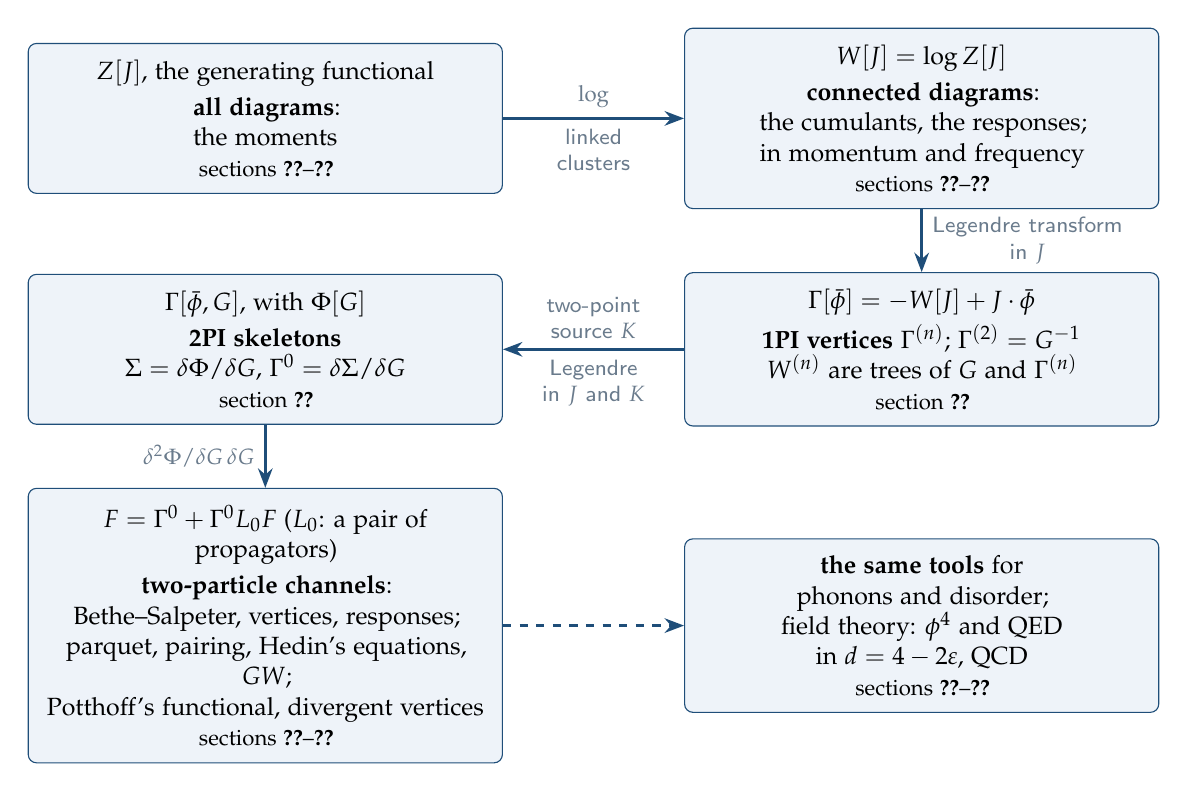
\begin{tikzpicture}[
    box/.style={draw=accent, fill=accentpale, rounded corners=3pt, text width=5.6cm, align=flush center, inner sep=6pt,
      font=\small},
    flow/.style={-{Stealth[length=7pt]}, line width=1.1pt, draw=accent},
    lab/.style={font=\footnotesize\sffamily, text=comment, align=center}]
\node[box] (Z) {$Z[J]$, the generating functional\\[2pt] \textbf{all diagrams}:\\ the moments\\
  {\footnotesize sections~\ref{sec:wick}--\ref{sec:bubbles}}};
\node[box, right=2.3cm of Z] (W) {$W[J]=\log Z[J]$\\[2pt] \textbf{connected diagrams}:\\ the cumulants, the responses;\\
  in momentum and frequency\\
  {\footnotesize sections~\ref{sec:cumulants}--\ref{sec:matsubara}}};
\node[box, below=0.8cm of W] (G1) {$\Gamma[\bar\phi]=-W[J]+J\cdot\bar\phi$\\[2pt] \textbf{1PI vertices} $\Gamma^{(n)}$;
  $\Gamma^{(2)}=G^{-1}$\\ $W^{(n)}$ are trees of $G$ and $\Gamma^{(n)}$\\ {\footnotesize section~\ref{sec:onepi}}};
\node[box, left=2.3cm of G1] (G2) {$\Gamma[\bar\phi,G]$, with $\Phi[G]$\\[2pt] \textbf{2PI skeletons}\\
  $\Sigma=\delta\Phi/\delta G$, $\Gamma^0=\delta\Sigma/\delta G$\\ {\footnotesize section~\ref{sec:twopi}}};
\node[box, below=0.8cm of G2] (P) {$F=\Gamma^0+\Gamma^0L_0F$ ($L_0$: a pair of propagators)\\[2pt] \textbf{two-particle channels}:\\
  Bethe--Salpeter, vertices, responses;\\ parquet, pairing, Hedin's equations, $GW$;\\ Potthoff's functional, divergent vertices\\ {\footnotesize sections~\ref{sec:twoparticle}--\ref{sec:beyond}}};
\node[box, right=2.3cm of P] (A) {\textbf{the same tools} for\\ phonons and disorder;\\ field theory: $\phi^4$ and QED\\
  in $d=4-2\varepsilon$, QCD\\
  {\footnotesize sections~\ref{sec:phonons}--\ref{sec:qcd}}};
\draw[flow] (Z) -- node[lab, above] {$\log$} node[lab, below] {linked\\clusters} (W);
\draw[flow] (W) -- node[lab, right] {Legendre transform\\in $J$} (G1);
\draw[flow] (G1) -- node[lab, above] {two-point\\source $K$} node[lab, below] {Legendre\\in $J$ and $K$} (G2);
\draw[flow] (G2) -- node[lab, left] {$\delta^2\Phi/\delta G\,\delta G$} (P);
\draw[flow, dashed] (P) -- (A);
\end{tikzpicture}\par}

\begin{itemize}[leftmargin=1.2em, itemsep=0pt]
\item $Z[J]$ \textbf{generates the moments}: its derivatives with respect to the sources, at zero source, are the
  correlation functions. For a free theory they are given by Wick's theorem; with an interaction, expanding $e^{-S_{\rm int}}$ gives
  perturbation theory, whose vacuum bubbles cancel in the normalized correlation functions.
\item $W=\log Z$ \textbf{generates the cumulants}, the connected correlation functions, sums of connected diagrams only
  (linked-cluster theorem). The connected two-point function is the full propagator $G$ (for fermions
  $G=-\langle T\psi\bar\psi\rangle_c$); its one-particle-irreducible part, with the legs removed
  (amputated), is the self-energy, and the Dyson equation $G=G_0+G_0\Sigma G$ rebuilds $G$.
\item \textbf{From diagrams to numbers}: in momentum and Matsubara frequency the sums over the internal frequencies
  are done by residues, and the continued self-energy obeys the optical theorem.
\item The \textbf{1PI effective action} $\Gamma[\bar\phi]$ of the mean field $\bar\phi=\langle\phi\rangle$ is the Legendre transform of $W$ in the source. Its pieces are the classical action $S[\bar\phi]$, the
  one loop $\frac12{\rm Tr}\ln S''[\bar\phi]$ and $\Gamma_1[\bar\phi]$, the 1PI vacuum diagrams with two or more loops in the background; its derivatives are
  the one-particle-irreducible vertices, and every connected function is a tree of full propagators and 1PI vertices.
\item The \textbf{2PI effective action} adds to $J$ a two-point source $K(x,y)$, coupled to $\frac12\phi(x)\phi(y)$ (to
  $\bar\psi(x)\psi(y)$ for fermions), and is the Legendre transform of $W[J,K]$ in both sources: the mean field $\bar\phi$ and
  the full propagator $G$ become the variables. The rest, $\Gamma_2[\bar\phi,G]$ ($\Phi[G]$, the Luttinger--Ward functional, at
  zero mean field), is defined exactly; expanded, it is minus the two-particle-irreducible skeleton diagrams. Its derivatives
  are the self-energy $\Sigma[G]$ and the irreducible vertex $\Gamma^0$; truncating $\Phi$ gives conserving approximations.
\item The response of $G$ to a one-body source, $L=\delta G/\delta U$, obeys by the chain rule the \textbf{Bethe--Salpeter equation}, with $\Gamma^0$ as its kernel. The \textbf{vertex of a one-body operator} (density, current) is the response of $G^{-1}$ to
  an external field coupled to that operator; it gives the response functions and the self-energy by the equation of
  motion.
\item The \textbf{parquet equations} sort the four-point vertex by the channel in which it is two-particle reducible: given
  the fully irreducible vertex, $\delta^4\Gamma[\bar\phi,G]/\delta\bar\phi^4$ at fixed $G$, they determine the vertex and, with the Schwinger--Dyson equation for $\Sigma$, the propagator together.
\item For fermions the Nambu propagator of the \textbf{superfield} $(\psi,\bar\psi)$, with its pairing blocks, as the
  variable gives the gap equation of BCS theory and the kernels of all three channels.
\item With the screened interaction $W$, the vertex gives \textbf{Hedin's equations}. A Hubbard--Stratonovich field makes $W$
  a propagator: the 2PI functional of $G$ and $W$ starts with the $GW$ approximation.
\item \textbf{Without the series}: one more Legendre transform, from $G$ to $\Sigma$, gives Potthoff's functional; where the
  irreducible vertex diverges, the functional becomes multivalued and the skeleton series can converge to the wrong
  branch. For
  \textbf{phonons and disorder}, functionals of two propagators, or of the averaged one, give the self-energies as derivatives.
\end{itemize}

\section*{Other names}\pdfbookmark[0]{Other names}{names}\label{sec:names}

The most common other names, in textbooks and papers, of the objects of Part~I, in the order of the sections;
signs and normalizations vary from book to book.

\smallskip
{\footnotesize\renewcommand{\arraystretch}{1.16}\setlength{\LTpre}{0pt}\setlength{\LTpost}{0pt}%
\begin{xltabular}{\linewidth}{@{}>{\raggedright\arraybackslash}p{4.9cm}@{\hspace{0.8em}}>{\raggedright\arraybackslash}X@{}}
\toprule
\textsf{\textbf{here}} & \textsf{\textbf{also called}}\\
\midrule
\endfirsthead
\toprule
\textsf{\textbf{here}} & \textsf{\textbf{also called}}\\
\midrule
\endhead
\bottomrule
\endlastfoot
$Z[J]$, generating functional & partition function in an external field; vacuum-to-vacuum amplitude\\
$W=\log Z$ & generating functional of the connected functions; at zero source, $-\Omega/T$\\
connected diagrams & linked diagrams; their sums are the cumulants\\
$G$, full propagator & Green function, two-point function\\
$F$, full vertex & reducible vertex, two-particle scattering amplitude\\
$\Sigma$, self-energy & mass operator, proper self-energy\\
skeleton diagrams & bold or dressed diagrams\\
$\chi$, density response & density--density correlation function, susceptibility\\
$L_0$, $\chi_0$ & particle--hole propagator; closed, the bubble (with free lines, Lindhard)\\
bubble chain & random-phase approximation (RPA), ring diagrams\\
$P$, polarization & irreducible polarization or polarizability; for photons, the vacuum polarization\\
imaginary time & Matsubara formalism, finite-temperature field theory\\
$\bar\phi=\langle\phi\rangle$, mean field & classical or background field; for bosons below $T_c$, the condensate\\
$\Gamma[\bar\phi]$, 1PI effective action & quantum effective action; at constant $\bar\phi$, the effective potential\\
$\Gamma^{(n)}$, 1PI vertices & proper vertices, vertex functions\\
$\Gamma[\bar\phi,G]$, 2PI effective action & Cornwall--Jackiw--Tomboulis (CJT) effective action\\
$\Phi[G]$, Luttinger--Ward functional & Baym's $\Phi$, $\Gamma_2$; truncated, a $\Phi$-derivable (conserving) approximation\\
$\Gamma^0=\delta\Sigma/\delta G$ & particle--hole irreducible vertex, Bethe--Salpeter kernel\\
$\Lambda$, vertex of the density & three-point vertex; its proper part $\tilde\Lambda$ is Hedin's $\Gamma$\\
$\Gamma_{\rm irr}$ & fully irreducible vertex, often written $\Lambda$\\
Schwinger--Dyson equation & Dyson--Schwinger equation, equation of motion of $G$\\
$\sfield=(\psi,\bar\psi)$, superfield & Nambu spinor\\
$\mathcal G$, Nambu propagator & Nambu--Gor'kov Green function, with normal and anomalous blocks\\
$\Delta$, gap function & anomalous self-energy, pairing field\\
$W$, screened interaction (not $W=\log Z$) & effective or dressed interaction\\
Hubbard--Stratonovich field & auxiliary field\\
$\mathcal F[\Sigma]$, Potthoff's functional & universal functional; $\Omega[\Sigma]$, the self-energy functional\\
Migdal's self-energy & Migdal--Eliashberg approximation; for disorder, the SCBA (self-consistent Born approximation)
\end{xltabular}\par}

\clearpage
\partheading{I}{Many-body theory}
% ------------------------------------------------------------------ 1
\section{The engine: functional derivatives}\label{sec:engine}

Everything in the package is built on a symbolic calculus of functional derivatives, which can be used on its own.
Its objects are sums of terms
\[
c\int_{z_1\cdots z_n} f(x,\dots;z_1,\dots,z_n)\;\theta_1\theta_2\cdots\theta_k ,
\]
a coefficient times an integral --- \pkg{IntegralOver[\dots, \{z1, \dots\}]} --- of a product of commuting factors $f$
and of Grassmann-odd factors $\theta_i$ in a definite order (written with \pkg{**}). A label such as $x$ stands for
whatever the problem needs: position, imaginary time, spin, orbital; the integral is the integral or sum over it.
Functions are arbitrary symbols, declared symmetric or antisymmetric if they are; sources are declared, commuting or
Grassmann; nothing else needs to be said about them. Every result is returned in a canonical form, described first.

\subsection{Expressions and their canonical form}

Delta functions are integrated as soon as they meet an integration variable; between two external labels they are kept,
and used to simplify. The integration variables of a result are renamed $z_1,z_2,\dots$ ($w_1,w_2,\dots$ in nested
integrals) by a canonical rule, so that two terms that differ only by the names of their integration variables, or by
the order of the arguments of symmetric functions, become identical and are added:
\begin{code}
SimplifyDiagrams[IntegralOver[M[x, u] DeltaFunction[u, v] M[v, y], {u, v}]]
SimplifyDiagrams[DeltaFunction[a, b] M[a, b] M[b, c]]
DeclareSymmetric[Q];
SimplifyDiagrams[IntegralOver[M[x, u] Q[u, v] M[v, y], {u, v}] +
    IntegralOver[M[x, s] Q[t, s] M[t, y], {s, t}]]
\end{code}
\begin{outputbox}
\vspace{-6pt}
\[
\formula{delta_integral},\qquad \formula{delta_external},\qquad \formula{same_diagram}
\]
\end{outputbox}
A term that changes sign under a symmetry of its own vanishes: here $Q$ is symmetric and the product of the two Grassmann
sources antisymmetric. The odd factors of a canonical term are sorted, with the sign of the permutation.
\begin{code}
DeclareGrassmannSource[eta, etabar];
SimplifyDiagrams[IntegralOver[Q[u, v] etabar[u] ** etabar[v], {u, v}]]
\end{code}
\begin{outputbox}
\vspace{-6pt}
\[
\formula{odd_term}
\]
\end{outputbox}
\pkg{DiagramTerms} lists the distinct terms with their weights, and \pkg{SimplifyDiagrams[a - b]} is \pkg{0} exactly when
\pkg{a} and \pkg{b} are equal: this is how every identity in this document is checked. Recognizing equal terms is what
makes the weights come out right; the algorithm, a colour refinement of the integration variables as in
graph-isomorphism programs, is described in section~\ref{sec:hood}.

\subsection{Derivatives with respect to commuting sources}

\pkg{FunctionalDerivative[F, s1, s2, \dots]} is $\delta/\delta s_1\,\delta/\delta s_2\cdots F$, the rightmost derivative
acting first. A functional of a source $J$, with a symmetric kernel $Q$ and a totally symmetric three-point kernel
$Q_3$:
\begin{code}
DeclareSource[J]; DeclareSymmetric[Q, Q3];
W = 1/2 IntegralOver[Q[x, y] J[x] J[y], {x, y}] +
    1/6 IntegralOver[Q3[x, y, z] J[x] J[y] J[z], {x, y, z}];
FunctionalDerivative[W, J[a]]
FunctionalDerivative[W, J[a], J[b]]
\end{code}
\begin{outputbox}
\vspace{-6pt}
\begin{align*}
\frac{\delta W}{\delta J(a)}&=\formula{first_derivative}\\
\frac{\delta^2 W}{\delta J(a)\,\delta J(b)}&=\formula{second_derivative}
\end{align*}
\end{outputbox}
The product rule gives three terms from the cubic part; since $Q_3$ is symmetric they are the same term, and their
weights add up to $\frac12$. Any function of the sources is differentiated by the chain rule --- powers, exponentials,
logarithms, the elementary functions, and functions left unspecified, whose derivatives are written $f'$, $f''$:
\begin{code}
FunctionalDerivative[f[IntegralOver[g[x] J[x], {x}]], J[a], J[b]]
FunctionalDerivative[Log[1 + IntegralOver[g[x] J[x], {x}]], J[a], J[b]]
FunctionalDerivative[Sqrt[IntegralOver[g[x] J[x]^2, {x}]], J[a]]
\end{code}
\begin{outputbox}
\vspace{-6pt}
\begin{gather*}
\formula{chain_rule},\qquad \formula{logarithm},\qquad \formula{square_root}
\end{gather*}
\end{outputbox}
A source can have several arguments, and an argument can run over discrete values, such as a spin projection:
$\delta J(x,s)/\delta J(y,t)=\delta(x,y)\,\delta(s,t)$, with $\delta(\uparrow,\uparrow)=1$ and $\delta(\uparrow,\downarrow)=0$.
\begin{code}
DeclareDiscreteIndexValues[{up, down}]; DeclareSymmetric[U];
spinFunctional = 1/2 IntegralOver[U[x, y] J[x, s] J[y, s], {x, y, s}];
FunctionalDerivative[spinFunctional, J[a, up], J[b, up]]
FunctionalDerivative[spinFunctional, J[a, up], J[b, down]]
\end{code}
\begin{outputbox}
\vspace{-6pt}
\[
\formula{spin_same}\qquad\text{and}\qquad\formula{spin_opposite}
\]
\end{outputbox}

\subsection{Grassmann sources}

For anticommuting sources the derivatives anticommute, and a left derivative that passes $k$ odd factors to reach its
source picks up the sign $(-1)^k$:
\begin{code}
bilinear = IntegralOver[M[x, y] etabar[x] ** eta[y], {x, y}];
FunctionalDerivative[bilinear, etabar[a], eta[b]]
FunctionalDerivative[bilinear, eta[b], etabar[a]]
FunctionalDerivative[Exp[bilinear], etabar[a], eta[b]]
\end{code}
\begin{outputbox}
\vspace{-6pt}
\begin{gather*}
\frac{\delta^2B}{\delta\bar\eta(a)\,\delta\eta(b)}=\formula{grassmann_ab},\qquad
\frac{\delta^2B}{\delta\eta(b)\,\delta\bar\eta(a)}=\formula{grassmann_ba}\qquad\Bigl(B=\int_{x,y}M(x,y)\,\bar\eta(x)\eta(y)\Bigr)\\[2pt]
\frac{\delta^2e^{B}}{\delta\bar\eta(a)\,\delta\eta(b)}=\formulasplit{grassmann_pair}
\end{gather*}
\end{outputbox}
In the canonical form the odd factors are sorted: $\bar\eta(x)\eta(y)=-\eta(y)\bar\eta(x)$. Grassmann-odd quantities that
are not sources, such as fermion fields written explicitly, are declared with \pkg{DeclareGrassmannOdd}.

\subsection{Implicit dependence}

Objects that depend on the sources only implicitly are differentiated by rules declared once with
\pkg{DeclareFunctionalDerivative}; the rules are then used everywhere, inside integrals and functions. A propagator in a
local source, $G=(G_0^{-1}-J)^{-1}$, obeys $\delta G(a,b)/\delta J(c)=G(a,c)\,G(c,b)$, and its second derivative follows:
\begin{code}
DeclareSymmetric[PropagatorOfJ];
DeclareFunctionalDerivative[PropagatorOfJ[p_, q_], J[r_],
    PropagatorOfJ[p, r] PropagatorOfJ[r, q]];
FunctionalDerivative[PropagatorOfJ[x, y], J[u], J[v]]
\end{code}
\begin{outputbox}
\vspace{-6pt}
\[
\frac{\delta^2 G(x,y)}{\delta J(u)\,\delta J(v)}=\formula{implicit}
\]
\end{outputbox}
The rules that generate the connected functions as trees of vertex functions (the tree expansion,
section~\ref{sec:trees}) are rules of this kind.

\subsection{Derivatives with respect to a propagator}

A source can be any function of any number of labels --- in particular a propagator. The Hartree--Fock functional
$\Phi=\frac12\int V(u,v)\,G(u,u)\,G(v,v)-\frac12\int V(u,v)\,G(u,v)\,G(v,u)$, differentiated once and twice with respect to
$G$, gives the Hartree--Fock self-energy $\Sigma(x,y)=\delta\Phi/\delta G(y,x)$ and the bare vertex, direct and exchange:
\begin{code}
DeclareSource[G]; DeclareSymmetric[V];
phiHF = 1/2 IntegralOver[V[u, v] G[u, u] G[v, v], {u, v}] -
    1/2 IntegralOver[V[u, v] G[u, v] G[v, u], {u, v}];
FunctionalDerivative[phiHF, G[y, x]]
FunctionalDerivative[phiHF, G[x4, x3], G[x2, x1]]
\end{code}
\begin{outputbox}
\vspace{-6pt}
\begin{align*}
\Sigma(x,y)&=\formula{hartree_fock}\\
\frac{\delta\Sigma(x_1,x_2)}{\delta G(x_4,x_3)}&=\formula{bare_vertex}
\end{align*}
\end{outputbox}
Differentiating a diagram with respect to $G$ opens one of its lines, in all possible ways; diagrams with external legs
follow in this way from the vacuum diagrams, as in the recursive graphical construction of Kleinert and
coworkers~\cite{Kleinert1982,KleinertPelsterKasteningBachmann2000,PelsterGlaum2003}. This is how \pkg{SelfEnergy} and
\pkg{IrreducibleVertex} work (section~\ref{sec:lw}). The declaration is not even needed: \pkg{FunctionalDerivative[F, G[x,
y]]} takes any object with two labels that is not a source --- a propagator, a self-energy, an interaction --- as the
variable, and differentiates through traces and logarithms of operators too (section~\ref{sec:lw}).

\subsection{Generating functionals}

A field is attached to its source with \pkg{DeclareField}: \pkg{DeclareField[phi, J]} makes the field $\phi(x)$ stand
for the derivative $\delta/\delta J(x)$. For any generating functional $Z$, \pkg{FieldDerivative[Z, \{phi[a], \dots\}]}
applies these derivatives, and \pkg{FieldExpectationValue}, with the same arguments, also divides by $Z$ at zero source.
With $Z=e^{W}$ and the cumulants $W_1$, $W_2$, $W_3$ of a non-Gaussian distribution, the third moment is expressed through
the cumulants, and the derivatives of $\log Z$ at zero source give the cumulants back:
\begin{code}
DeclareField[phi, J]; DeclareSymmetric[W2, W3];
Z = Exp[IntegralOver[W1[x] J[x], {x}] + 1/2 IntegralOver[W2[x, y] J[x] J[y], {x, y}] +
    1/6 IntegralOver[W3[x, y, z] J[x] J[y] J[z], {x, y, z}]];
FieldExpectationValue[Z, {phi[a], phi[b], phi[c]}]
SetSourcesToZero[FunctionalDerivative[Log[Z], J[a], J[b], J[c]]]
\end{code}
\begin{outputbox}
\vspace{-6pt}
\begin{gather*}
\langle\phi(a)\phi(b)\phi(c)\rangle=\formulasplit{moments}\\
\frac{\delta^3\log Z}{\delta J(a)\,\delta J(b)\,\delta J(c)}\Big|_{J=0}=\formula{cumulants}
\end{gather*}
\end{outputbox}
For a Gaussian $Z_0$ the expectation values are given by Wick's theorem, and the results are Feynman diagrams
(section~\ref{sec:wick}).

\begin{keypoint}
Every formula in the boxes above was written by \pkg{ExpressionToLaTeX}, which turns an expression of the package into
\LaTeX{} (\pkg{"Names" -> \{PropagatorOfJ -> "G"\}} gave $G$ its name in the implicit derivative); \pkg{DiagramToTikZ}
does the same for pictures (section~\ref{sec:pictures}). In Mathematica the results are displayed in a compact notation,
$\int_{z_1z_2}$, $\delta_{xy}$, which remains valid input.
\end{keypoint}

% ------------------------------------------------------------------ 2
\section{Generating functionals and Wick's theorem}\label{sec:wick}

\paragraph{From the path integral to derivatives} The generating functional of a field theory is the path integral
$Z[J]=\int\!D\phi\;e^{-S[\phi]+J\cdot\phi}$, with $J\cdot\phi=\int_xJ(x)\phi(x)$ --- in statistical physics the partition function in an
external field $J$, in real-time field theory the vacuum-to-vacuum amplitude (the other names of the objects of this
document are collected on page~\pageref{sec:names}). A derivative with respect to the source brings
down a field, $\delta e^{J\cdot\phi}/\delta J(a)=\phi(a)\,e^{J\cdot\phi}$, so that the derivatives of $Z$ at $J=0$ are the
expectation values --- the moments of the distribution $e^{-S}$:
\[
\langle\phi_a\phi_b\cdots\rangle=\frac1{Z[0]}\,\frac{\delta^nZ}{\delta J_a\,\delta J_b\cdots}\Big|_{J=0},\qquad
\frac{\delta^nW}{\delta J_a\,\delta J_b\cdots}\Big|_{J=0}=\langle\phi_a\phi_b\cdots\rangle_c,\quad W=\log Z,
\]
for $n$ fields $\phi_a\phi_b\cdots$,
and, as for any probability distribution, the derivatives of the logarithm are the cumulants~\cite{Kubo1962}, the
connected correlation functions: $\langle\phi_a\rangle_c=\langle\phi_a\rangle$, $\langle\phi_a\phi_b\rangle_c=\langle\phi_a\phi_b\rangle-\langle\phi_a\rangle\langle\phi_b
\rangle$, and so on (section~\ref{sec:cumulants}). At a non-zero source the same derivatives, with $Z[J]$ in
place of $Z[0]$, are the expectation values in the presence of an external field $J$.
Write the action as a quadratic part and an interaction, $S=\frac12\,\phi\cdot D_0^{-1}\cdot\phi+S_{\rm int}[\phi]$. Inside the
integral a field is a derivative of the source term, $\phi(x)\,e^{J\cdot\phi}=\frac{\delta}{\delta J(x)}\,e^{J\cdot\phi}$, so that the
interaction can be taken out of the integral as a differential operator, and what is left is a Gaussian integral, done
once and for all:
\[
Z[J]=e^{-S_{\rm int}[\delta/\delta J]}\int\!D\phi\;e^{-\frac12\phi\cdot D_0^{-1}\cdot\phi+J\cdot\phi}
=\mathcal N\,e^{-S_{\rm int}[\delta/\delta J]}\;e^{\frac12J\cdot D_0\cdot J}.
\]

\paragraph{Perturbation theory as differentiation} From here on everything is differentiation. Each derivative acting on the Gaussian either brings down a factor $D_0\cdot J$
or, acting on a factor brought down before, turns it into a propagator $D_0$ between two points --- Wick's theorem --- and expanding
$e^{-S_{\rm int}[\delta/\delta J]}$ in powers of the interaction generates every Feynman diagram, with its weight. For
fermions the fields and the sources are Grassmann variables, and the same construction
holds~\cite{Berezin1966,NegeleOrland} (paragraph \emph{Free fields} below). The
engine carries out these derivatives literally (for the path integral and its Gaussian integrals
see~\cite{NegeleOrland,ZinnJustin2002,AltlandSimons,PeskinSchroeder}).

\paragraph{The weights of the pictures} In the pictures an interaction line stands for $-V$ and a vertex for minus its
coupling ($-\lambda$ in $\phi^4$ theory): the minus sign comes from expanding $e^{-S_{\rm int}}$. The number written in
front of a picture, times the values of its lines and vertices, is the term, with the internal points integrated over.

\paragraph{Free fields} A Gaussian generating functional $Z_0[J]=\exp\bigl(\tfrac12\,J\cdot D_0\cdot J\bigr)$ generates the free correlation
functions, $\langle\phi_a\phi_b\cdots\rangle_0=\delta^n Z_0/\delta J_a\,\delta J_b\cdots\bigr|_{J=0}$~\cite{Wick1950,NegeleOrland}. The product and
chain rules produce all the terms, and at zero source only the complete pairings survive. The results are sums of
diagrams, shown as pictures drawn by the package;
the names of the functions are explicit in the input, and can be displayed as short symbols in the output
(\pkg{DeclareDisplayName}).
\begin{code}
DeclareSymmetric[FreePropagator];
FreeBosonGeneratingFunctional = Exp[1/2 IntegralOver[J[x] FreePropagator[x, y] J[y],
    {x, y}]];
fourPoint = SetSourcesToZero[FunctionalDerivative[FreeBosonGeneratingFunctional,
    J[a], J[b], J[c], J[d]]];
DiagramPlot[fourPoint, {a, b, c, d}]
\end{code}
\figuresum{\langle\phi_a\phi_b\phi_c\phi_d\rangle_0}{pairings}
Fermions are described by Grassmann fields and sources. In many-body theory a label $x$ includes the imaginary time
$\tau_x\in[0,\beta)$ of the thermal path integral at the temperature $1/\beta$ (section~\ref{sec:matsubara}), and $T$
orders the fields by it, the latest on the left, with a factor $-1$ for each exchange of two fermion
fields~\cite{FetterWalecka,NegeleOrland}: the path integral gives these time-ordered products directly. With the
convention $G_0(x,y)=-\langle T\,\psi(x)\bar\psi(y)\rangle_0$ the free generating functional is
$Z_0[\eta,\bar\eta]=\exp(-\bar\eta\cdot G_0\cdot\eta)$, and the fields stand for the derivatives
$\psi\leftrightarrow\delta/\delta\bar\eta$, $\bar\psi\leftrightarrow-\delta/\delta\eta$. The sign of the exchange term is not
put in by hand: it comes out of the Grassmann algebra.
\begin{code}
DeclareGrassmannSource[eta, etabar]; DeclareDirectedPropagator[BareGreenFunction];
DeclareField[psi, etabar]; DeclareField[psibar, eta, -1];
FreeFermionGeneratingFunctional = Exp[-IntegralOver[
    BareGreenFunction[x, y] etabar[x] ** eta[y], {x, y}]];
GaussianExpectationValue[FreeFermionGeneratingFunctional,
    {psi[a], psi[b], psibar[c], psibar[d]}]
\end{code}
\figuresum{\langle\psi_a\psi_b\bar\psi_c\bar\psi_d\rangle_0}{fermion_four_point}
The fermionic six-point function $\langle\psi\psi\psi\bar\psi\bar\psi\bar\psi\rangle_0$ is a $3\times3$ determinant,
$3!=6$ terms; the bosonic $\langle\phi^6\rangle_0$ has $15$ pairings. For Gaussian functionals
\pkg{GaussianExpectationValue} uses Wick's theorem as a sum over pairings, which is much faster; literal differentiation
(\pkg{"Method" -> "Differentiation"}) gives the same results, as the test suite checks, and works for any generating
functional.

\paragraph{What a label is} Nothing in the diagrams depends on what a label is (section~\ref{sec:engine}): the same diagrams
hold in any dimension, for a lattice or the continuum, at zero or finite temperature in imaginary
time~\cite{Matsubara1955} (the Matsubara formalism, thermal or Euclidean field theory in particle physics), and, with factors of $i$ in the weights from $e^{iS}$ in place of $e^{-S}$, in real time and
out of equilibrium, where the times run on the closed Schwinger--Keldysh
contour~\cite{Schwinger1961,Keldysh1964,Kamenev2011,StefanucciVanLeeuwen2013}; only the meaning of the contracted labels
changes. A propagator at equal labels, $G(z,z)$, stands for $G(z,z^+)$, the
density; an instantaneous interaction is $V(x,y)=v(\mathbf r_x-\mathbf r_y)\,\delta(\tau_x-\tau_y)$ (in
momentum space $v_q$, the Fourier transform of $v$, with $v_q=4\pi e^2/q^2$ for the Coulomb interaction), a retarded one
(phonons) is just another function; for a spin-independent interaction spin need not appear, and each closed fermion
loop then carries the factor $2s+1$ on evaluation. The results are exact symbolic expressions, with their signs and
weights, ready for any representation. Throughout, $\hbar=k_B=1$; the electron gas is written in Gaussian units, QED
(section~\ref{sec:qed}) in Heaviside--Lorentz units. Section~\ref{sec:matsubara} turns the diagrams into momentum
and Matsubara frequency.

% ------------------------------------------------------------------ 3
\Needspace{10\baselineskip}
\section{Interactions: vacuum bubbles and the linked-cluster theorem}\label{sec:bubbles}

With an interaction the generating functional is $Z[J]=e^{-S_{\rm int}[\delta/\delta J]}\,Z_0[J]$ (section~\ref{sec:wick}),
up to a constant. For $\phi^4$ theory, $S_{\rm int}=\frac\lambda{4!}\int_z\phi^4$, the package applies this operator
as it stands, one order at a time. In this document $\phi^4$ theory is worked out to third order in $\lambda$
(\pkg{phi4Z} is $Z[J]$ to that order, at any source) and the electron gas to third order in $V$:
\begin{code}
DeclareField[phi, J];
Phi4Vertex = lambda/24 IntegralOver[phi[z]^4, {z}];   (* S_int, used below *)
DeclareCoupling[lambda];         (* in the pictures each vertex stands for -lambda *)
applyInteraction[F_] := SimplifyDiagrams[
    -lambda/24 IntegralOver[FunctionalDerivative[F, J[z], J[z], J[z], J[z]], {z}]];
firstOrder = applyInteraction[FreeBosonGeneratingFunctional];
secondOrder = applyInteraction[firstOrder]; thirdOrder = applyInteraction[secondOrder];
phi4Z = FreeBosonGeneratingFunctional + firstOrder + secondOrder/2 + thirdOrder/6;
SetSourcesToZero[phi4Z]
\end{code}
At zero source $Z/Z_0=\langle e^{-S_{\rm int}}\rangle_0$ is the sum of all the vacuum diagrams, disconnected ones included,
each with its symmetry factor~\cite{PeskinSchroeder,CvitanovicLautrupPearson1978}. Here and below, a sum of several orders
is written order by order, in coloured bands with the order in the interaction on the left:
\begin{ordersum}{\frac{Z}{Z_0}}
\orderrow{\lambda^0}{phi4_vacuum_0}
\orderrow{\lambda}{phi4_vacuum_1}
\orderrow{\lambda^2}{phi4_vacuum_2}
\orderrow{\lambda^3}{phi4_vacuum_3}
\end{ordersum}
\paragraph{Symmetry factors} The coefficient of a diagram is what the expansion puts in front, at order $n$
$(-\lambda)^n/(n!\,(4!)^n)$, times the number of Wick contractions that give the same picture. It is $(-\lambda)^n/S$, and
the weight written with the picture, each vertex standing for $-\lambda$, is $1/S$, where the symmetry factor $S$ is the number of permutations of the vertices and of
the lines that leave the diagram unchanged~\cite{PeskinSchroeder,CvitanovicLautrupPearson1978}: the figure eight has
$S=2\cdot2\cdot2=8$ (its two loops can be reversed and exchanged), the two vertices joined by four lines (the first
diagram at $\lambda^2$) $S=2\cdot4!=48$, the tadpole on a propagator $S=2$, the sunset $S=3!=6$. The package does not use
this rule: it counts the contractions as derivatives, and the canonical form adds up the copies of each
diagram.

\paragraph{Products of connected pieces: the linked-cluster theorem} Most of these diagrams are disconnected, and a
disconnected diagram is the product of its connected pieces: the pieces share no line, so the integrals over their vertices
are independent. The weights multiply too. At order $n$ the exponential brings $1/n!$, and a diagram whose pieces have
$n_1,n_2,\dots$ vertices arises from the $n!/(n_1!\,n_2!\cdots)$ ways of choosing which vertices go to which piece, each
with the contractions of every piece: the $n!$ cancels, and each piece keeps the $1/n_i!$ of its own order --- its own
weight. The one exception is a piece that occurs $k$ times: two choices that differ only by exchanging the vertices of two
identical pieces give the same contractions, one term and not two, so $k$ identical pieces carry an extra $1/k!$. This is
how the exponential series counts: $\exp(c_1+c_2+\cdots)$ of the connected vacuum diagrams $c_i$, expanded, contains every
collection of them once, with the product of their weights and $1/k!$ for a diagram repeated $k$ times. Hence
\[
\frac{Z}{Z_0}=\exp\Bigl(\sum\text{connected vacuum diagrams}\Bigr),\qquad
\log\frac{Z}{Z_0}=\sum\text{connected vacuum diagrams},
\]
the linked-cluster theorem~\cite{Goldstone1957,Hubbard1957,AbrikosovGorkovDzyaloshinski} (Goldstone's linked-diagram
theorem). With $c_n$ the connected diagrams of order $\lambda^n$, $Z/Z_0=1+c_1+\bigl(c_2+\frac1{2!}c_1^2\bigr)+\bigl(c_3+c_1c_2+
\frac1{3!}c_1^3\bigr)+\dots$; in pictures, the rows $\lambda^2$ and $\lambda^3$ of the sum above are
\begin{align*}
\frac{Z}{Z_0}\Big|_{\lambda^2}&=\Bigl(\inputfigure{phi4_connected_second}\Bigr)+\frac1{2!}\Bigl(\frac18\inputfigure{phi4_eight}\Bigr)^2,\\
\frac{Z}{Z_0}\Big|_{\lambda^3}&=\Bigl(\inputfigure{phi4_connected_third}\Bigr)
+\frac18\inputfigure{phi4_eight}\,\Bigl(\inputfigure{phi4_connected_second}\Bigr)+\frac1{3!}\Bigl(\frac18\inputfigure{phi4_eight}\Bigr)^3.
\end{align*}
Counted by hand: a vertex closes its four lines into a figure eight in 3 ways, so the eight has the weight $3/4!=\frac18$,
and two vertices are joined by four lines in $4!$ ways, with the weight $\frac1{2!}\,4!/(4!)^2=\frac1{48}$. Two figure eights
come from the $3\cdot3$ contractions in which each vertex closes on itself: the two pieces are identical, there is no
choice of which vertex makes which eight, and the $\frac1{2!}$ of the exponential stays. The eight beside the two vertices
joined by four lines has 3 choices of the vertex of the eight, which turn the $\frac1{3!}$ of the exponential into the
$\frac1{2!}$ of the piece of second order:
\[
\frac1{2!}\,\frac{3\cdot3}{(4!)^2}=\frac1{128}=\frac1{2!}\Bigl(\frac18\Bigr)^2,\qquad
\frac1{3!}\,\frac{3\cdot3\cdot4!}{(4!)^3}=\frac1{384}=\frac18\cdot\frac1{48};
\]
in the same way the eight beside the other diagram of second order has $\frac1{128}=\frac18\cdot\frac1{16}$, and three
eights $\frac1{3072}=\frac1{3!}\bigl(\frac18\bigr)^3$. The package checks the theorem on the series computed above by derivatives: with $z_n$ the vacuum diagrams of order
$\lambda^n$ (\pkg{vacuum1}, \pkg{vacuum2}, \pkg{vacuum3} in the code), the logarithm of
$1+z_1+z_2+z_3$, expanded to $\lambda^3$, is the sum of the connected diagrams among them, which
\pkg{ConnectedDiagrams} picks out:
\begin{code}
{vacuum1, vacuum2, vacuum3} = {SetSourcesToZero[firstOrder],
    SetSourcesToZero[secondOrder]/2, SetSourcesToZero[thirdOrder]/6};
connectedVacuum = ConnectedDiagrams[vacuum1 + vacuum2 + vacuum3, {}]
SimplifyDiagrams[vacuum1 + vacuum2 + vacuum3 - vacuum1^2/2 - vacuum1 vacuum2
    + vacuum1^3/3 - connectedVacuum]
\end{code}
\begin{ordersum}{\log\frac{Z}{Z_0}}
\orderrow{\lambda}{phi4_log_vacuum_1}
\orderrow{\lambda^2}{phi4_log_vacuum_2}
\orderrow{\lambda^3}{phi4_log_vacuum_3}
\end{ordersum}
\pkg{ConnectedVacuumDiagrams[FreeBosonGeneratingFunctional, Phi4Vertex, 3]} computes the same sum directly.
\begin{result}
$\log(1+z_1+z_2+z_3)$ minus the connected diagrams of $Z/Z_0$, to $\lambda^3$: \val{CheckPhi4LinkedCluster}\\
$\exp(c_1+c_2+c_3)-Z/Z_0$, to $\lambda^3$: \val{CheckPhi4ExponentialOfTheConnectedDiagrams}\\
\pkg{ConnectedVacuumDiagrams} minus the connected diagrams of $Z/Z_0$: \val{CheckPhi4ConnectedVacuumShortcut}
\end{result}

\paragraph{External points: the bubbles cancel} A correlation function is normalized by $Z$. Its numerator
$\langle\phi_a\phi_b\,e^{-S_{\rm int}}\rangle_0$, the second derivative of $Z/Z_0$ at $J=0$, contains the vacuum diagrams as
factors --- the figure eight beside the free propagator and beside the tadpole, and so on:
\begin{ordersum}{\langle\phi_a\phi_b\,e^{-S_{\rm int}}\rangle_0}
\orderrow{\lambda^0}{phi4_numerator_0}
\orderrow{\lambda}{phi4_numerator_1}
\orderrow{\lambda^2}{phi4_numerator_2}
\orderrow{\lambda^3}{phi4_numerator_3}
\end{ordersum}
The counting is the same: a diagram of the numerator is a part joined to the external points times vacuum pieces. At
order $n$, the $n!/(m!\,(n-m)!)$ ways of choosing which $m$ vertices go to the part joined to $a$ and $b$ turn the $1/n!$ of
the exponential into $1/m!$ for that part and $1/(n-m)!$ for the vacuum pieces, and the sum of all the diagrams is a
product,
\[
\langle\phi_a\phi_b\,e^{-S_{\rm int}}\rangle_0=\Bigl(\inputfigure{phi4_propagator_0}\;\inputfigure{phi4_propagator_1}+\cdots\Bigr)
\Bigl(1\;\inputfigure{phi4_vacuum_1}+\cdots\Bigr)=\langle\phi_a\phi_b\rangle\,\frac{Z}{Z_0},
\]
so the bubbles cancel against the normalization: $\langle\phi_a\phi_b\rangle=\langle\phi_a\phi_b\,e^{-S_{\rm int}}\rangle_0/\langle
e^{-S_{\rm int}}\rangle_0$ is the sum of the diagrams without vacuum bubbles. The package checks the product order by order;
\pkg{PerturbativeCorrelationFunction} computes $\langle\phi_a\phi_b\rangle$ directly, and never generates the bubbles:
\begin{code}
numerator = SetSourcesToZero[FunctionalDerivative[phi4Z, J[a], J[b]]];
phi4Propagator = PerturbativeCorrelationFunction[FreeBosonGeneratingFunctional,
    {phi[a], phi[b]}, Phi4Vertex, 3]
SimplifyDiagrams[OrderPart[numerator - DropVacuumBubbles[numerator, {a, b}]
    (1 + vacuum1 + vacuum2 + vacuum3), lambda, {0, 1, 2, 3}]]
\end{code}
\begin{ordersum}{\langle\phi_a\phi_b\rangle}
\orderrow{\lambda^0}{phi4_propagator_0}
\orderrow{\lambda}{phi4_propagator_1}
\orderrow{\lambda^2}{phi4_propagator_2}
\orderrow{\lambda^3}{phi4_propagator_3}
\end{ordersum}
\begin{result}
The numerator minus its diagrams without bubbles times $Z/Z_0$, orders $\lambda^0,\dots,\lambda^3$: \val{CheckPhi4NumeratorFactorizes}\\
\pkg{PerturbativeCorrelationFunction} minus the diagrams of the numerator without bubbles: \val{CheckPhi4PropagatorShortcut}
\end{result}

\paragraph{Fermions: the electron gas} Electrons with a two-body interaction $V(x,y)$ between densities --- the Coulomb
interaction or any other --- have the interaction
\[
S_{\rm int}=\tfrac12\textstyle\int_{x,y}V(x,y)\,\bar\psi(x)\bar\psi(y)\psi(y)\psi(x).
\]
The same steps as for $\phi^4$ theory, with $e^{-S_{\rm int}[-\delta/\delta\eta,\,\delta/\delta\bar\eta]}$ applied to
$Z_0[\eta,\bar\eta]$, give the vacuum diagrams, disconnected ones included: \val{CountsElectronVacuumFull1},
\val{CountsElectronVacuumFull2} and \val{CountsElectronVacuumFull3} at orders $V$, $V^2$ and $V^3$, every closed fermion
loop with a factor $-1$:
\begin{code}
DeclareSymmetric[InteractionPotential]; DeclareInteractionLine[InteractionPotential];
CoulombVertex = 1/2 IntegralOver[InteractionPotential[x, y]
    psibar[x] ** psibar[y] ** psi[y] ** psi[x], {x, y}];   (* S_int, used below *)
applyInteraction[F_] := SimplifyDiagrams[-1/2 IntegralOver[InteractionPotential[u, v]
    FunctionalDerivative[F, eta[u], eta[v], etabar[v], etabar[u]], {u, v}]];
firstOrder = applyInteraction[FreeFermionGeneratingFunctional];
secondOrder = applyInteraction[firstOrder]; thirdOrder = applyInteraction[secondOrder];
SetSourcesToZero[FreeFermionGeneratingFunctional + firstOrder + secondOrder/2 +
    thirdOrder/6]
\end{code}
\begin{ordersum}{\frac{Z}{Z_0}}
\orderrow{V^0}{electron_vacuum_full_0}
\orderrow{V}{electron_vacuum_full_1}
\orderrow{V^2}{electron_vacuum_full_2}
\orderrow{V^3}{electron_vacuum_full_3}
\end{ordersum}
The interaction lines carry two different points, so most weights are $\pm1$; the vacuum diagrams keep factors such as
$\frac12$ (Hartree and Fock): the symmetry of the diagram under the exchange of the two ends of its interaction line.
The counting is that of $\phi^4$ theory, and so are the theorem and the cancellation of the bubbles; the signs do not spoil
the products. A vacuum piece contains an even number of Grassmann fields --- four at each vertex, contracted in pairs within
the piece --- so the pieces commute with each other, and the sign of a diagram is the product of the signs of its pieces,
$(-1)^{n_L}=\prod_i(-1)^{n_{L,i}}$ for pieces with $n_{L,i}$ closed loops: the sign of a loop belongs to its connected piece. At second
order, the products of the Fock and Hartree diagrams of first order:
\begin{gather*}
\frac18\inputfigure{electron_vacuum_fock}\inputfigure{electron_vacuum_fock}=\frac1{2!}\Bigl(-\frac12\inputfigure{electron_vacuum_fock}\Bigr)^2,
\qquad
-\frac14\inputfigure{electron_vacuum_fock}\inputfigure{electron_vacuum_hartree}=\Bigl(-\frac12\inputfigure{electron_vacuum_fock}\Bigr)
\Bigl(\frac12\inputfigure{electron_vacuum_hartree}\Bigr),
\\
\frac18\inputfigure{electron_vacuum_hartree}\inputfigure{electron_vacuum_hartree}=\frac1{2!}\Bigl(\frac12\inputfigure{electron_vacuum_hartree}\Bigr)^2.
\end{gather*}
So the logarithm keeps the connected vacuum diagrams, $\log(Z/Z_0)=-\beta(\Omega-\Omega_0)$, where
$Z=\operatorname{tr}e^{-\beta(H-\mu N)}$ and $\Omega=-\beta^{-1}\log Z$ is the grand potential. As for $\phi^4$ theory,
with \pkg{vacuum1}, \pkg{vacuum2}, \pkg{vacuum3} now the vacuum diagrams of the electron gas:
\begin{code}
{vacuum1, vacuum2, vacuum3} = {SetSourcesToZero[firstOrder],
    SetSourcesToZero[secondOrder]/2, SetSourcesToZero[thirdOrder]/6};
connectedVacuum = ConnectedDiagrams[vacuum1 + vacuum2 + vacuum3, {}];
vacuum = ConnectedVacuumDiagrams[FreeFermionGeneratingFunctional, CoulombVertex, 3]
\end{code}
\begin{ordersum}{\log\frac{Z}{Z_0}}
\orderrow{V}{vacuum_1}
\orderrow{V^2}{vacuum_2}
\orderrow{V^3}{vacuum_3}
\end{ordersum}
\begin{result}
$\log(1+z_1+z_2+z_3)$ minus the connected diagrams of $Z/Z_0$, to $V^3$: \val{CheckElectronLinkedCluster}\\
\pkg{ConnectedVacuumDiagrams} minus the same: \val{CheckElectronConnectedVacuumShortcut}
\end{result}
The numerator of the Green function, $-\langle T\,\psi_x\bar\psi_y\,e^{-S_{\rm int}}\rangle_0$, contains the vacuum diagrams as
factors (\val{CountsElectronNumerator2} diagrams at second order, drawn here to that order):
\begin{ordersum}{-\langle T\,\psi_x\bar\psi_y\,e^{-S_{\rm int}}\rangle_0}
\orderrow{V^0}{electron_numerator_0}
\orderrow{V}{electron_numerator_1}
\orderrow{V^2}{electron_numerator_2}
\end{ordersum}
and is the Green function, without vacuum bubbles, times $Z/Z_0$. So the Green function
\[
G(x,y)=-\frac{\langle T\,\psi(x)\bar\psi(y)\,e^{-S_{\rm int}}\rangle_0}{\langle e^{-S_{\rm int}}\rangle_0},
\]
here to third order, has no vacuum bubbles:
\begin{code}
greenFunction = -PerturbativeCorrelationFunction[FreeFermionGeneratingFunctional,
    {psi[x], psibar[y]}, CoulombVertex, 3];
DiagramPlot[greenFunction, {x, y}]
\end{code}
$G$ has \val{CountsG1}, \val{CountsG2} and \val{CountsG3} diagrams of first, second and third order. An arrow from $y$ to
$x$ is $G_0(x,y)$, the wavy line stands for $-V$, and every diagram has the weight $\pm1$: a diagram with $n_L$ closed
fermion loops has the sign $(-1)^{n_L}$ (its coefficient, at order $n$, is $(-1)^{n+n_L}$), which the package obtains from the
Grassmann algebra, not from this rule:
\begin{ordersum}{G(x,y)}
\orderrow{V^0}{green_function_0}
\orderrow{V}{green_function_1}
\orderrow{V^2}{green_function_2}
\orderrow{V^3}{green_function_3}
\end{ordersum}
\begin{result}
The numerator minus its diagrams without bubbles times $Z/Z_0$, orders $V^0$, $V$, $V^2$: \val{CheckElectronNumeratorFactorizes}\\
Its diagrams without bubbles minus $G$, to $V^2$: \val{CheckElectronGWithoutBubbles}
\end{result}

\paragraph{Diagrams at a non-zero source} The series can also be drawn before any derivative is taken, and the
linked-cluster theorem holds at any source. For $\phi^4$ theory write $Z[J]=Z_0[J]\,\bigl(1+z_1[J]+z_2[J]+\dots\bigr)$, with $Z_0[J]$ set aside; a line is a free propagator $D_0$ and a crossed circle a source $J$, integrated over its position.
To first order there is one diagram with no source, one with two sources and one with four:
\figuresum{z_1[J]}{phi4_z_source_1}
and to second order \val{CountsPhi4ZAndWAtASource2} diagrams, with zero to eight sources, many of them products of
disconnected pieces:
\figuresum{z_2[J]}{phi4_z_source_2}
A derivative $\delta/\delta J(a)$ removes a source and leaves an external point $a$ in its place; at $J=0$ only the diagrams
with as many sources as derivatives survive. So $\delta^2Z/\delta J_a\delta J_b$ at $J=0$ collects the diagrams with two
sources --- the other diagrams of the numerator above --- and the free propagator times the diagrams with none,
the vacuum bubbles; $\delta^4/\delta J^4$ the diagrams with four sources, and so on. Taking the logarithm,
$W[J]=\log Z[J]=\frac12J\cdot D_0\cdot J+w_1[J]+w_2[J]+\dots$ with $w_1=z_1$ and $w_2=z_2-\frac12z_1^2$: the square of the
first order removes exactly the products of disconnected pieces, and $W$ keeps the \val{CountsPhi4ZAndWAtASource3} connected
diagrams --- the linked-cluster theorem, at any source:
\Needspace{6\baselineskip}
\figuresum{w_2[J]}{phi4_w_source_2}
\begin{result}
$w_2[J]$ minus its connected diagrams: \val{CheckPhi4WAtASourceConnected}
\end{result}
The same holds for the electron gas, with
$Z[\eta,\bar\eta]=Z_0\,(1+z_1+z_2+\dots)$. A line is a free propagator $G_0$, and a crossed circle a source: $\eta$ where a line
starts, $\bar\eta$ where it ends. To first order there are the two vacuum diagrams, Hartree and Fock, the same two opened
into a line between two sources, and the interaction between two lines:
\figuresum{z_1[\eta,\bar\eta]}{electron_z_source_1}
To second order there are \val{CountsElectronZAndWAtASource2} diagrams:
\figuresum{z_2[\eta,\bar\eta]}{electron_z_source_2}
and $W=\log Z$ keeps the \val{CountsElectronZAndWAtASource3} connected ones:
\figuresum{w_2[\eta,\bar\eta]}{electron_w_source_2}
\begin{result}
$w_2[\eta,\bar\eta]$ minus its connected diagrams: \val{CheckElectronWAtASourceConnected}
\end{result}

% ------------------------------------------------------------------ 4
\section{Moments and cumulants: \texorpdfstring{$W=\log Z$}{W = log Z}}\label{sec:cumulants}

$Z[J]$ generates the moments, the full correlation functions; $W[J]=\log Z[J]$ (at zero source $-\Omega/T$, minus the
grand potential over the temperature; in field theory the Schwinger functional, in probability the cumulant generating
function) generates the cumulants, the
\emph{connected} correlation functions $W^{(n)}=\delta^nW/\delta J^n$, sums of connected diagrams only
(section~\ref{sec:engine} shows the algebra on a non-Gaussian distribution).

\paragraph{Why the logarithm} The derivatives of $Z=e^W$ show it. $\delta e^W/\delta J_a=W_a\,e^W$, and every further derivative
either acts on the exponential, bringing down $W_b$ --- a new block --- or on a derivative of $W$ already there, turning $W_a$
into $W_{ab}$ --- the point $b$ joins the block of $a$:
\[
\frac1Z\,\frac{\delta^2Z}{\delta J_a\,\delta J_b}=W_{ab}+W_aW_b,\qquad
\frac1Z\,\frac{\delta^3Z}{\delta J_a\,\delta J_b\,\delta J_c}=W_{abc}+W_{ab}W_c+W_{ac}W_b+W_{bc}W_a+W_aW_bW_c.
\]
After $n$ derivatives, $\delta^nZ/Z$ is the sum over all the partitions of the $n$ points into blocks, each block a
cumulant: the moments in terms of the cumulants. It is the exponential series of section~\ref{sec:bubbles} again, with
the cumulants in place of the connected pieces; the points are all different, so no two blocks are alike, and each
partition comes once, with the coefficient 1 (no $1/k!$). Read
backwards, $W^{(n)}$ is the moment minus every way of splitting its points into smaller blocks, and this removes exactly
the disconnected diagrams. In $\phi^4$ theory at zero source the odd cumulants vanish, and the four-point function is the
connected four-point function $W^{(4)}$ plus the three pairings of full propagators $W^{(2)}=\langle\phi\phi\rangle$ (double
lines); the package draws it from the derivatives of $e^W$:
\begin{code}
DeclareSymmetric[ConnectedTwoPoint, ConnectedFourPoint];
DeclareLineStyle[ConnectedTwoPoint, "Double"];
DeclareBlob[ConnectedFourPoint, "\\scriptstyle W^{(4)}", "Fill" -> "White"];
expW = Exp[1/2 IntegralOver[ConnectedTwoPoint[x, y] J[x] J[y], {x, y}] +
    1/24 IntegralOver[ConnectedFourPoint[x, y, u, v] J[x] J[y] J[u] J[v],
        {x, y, u, v}]];
FieldExpectationValue[expW, {phi[a], phi[b], phi[c], phi[d]}]
\end{code}
\figuresum{\langle\phi_a\phi_b\phi_c\phi_d\rangle}{phi4_partitions}
Here $W^{(4)}$ is a blob (\pkg{DeclareBlob}), with its name written inside. All the blobs in this document are filled
by one rule: a vertex function the more densely the more diagrams it contains --- the fully irreducible vertex dotted,
the irreducible parts hatched, the full vertex functions cross-hatched~--- and a correlation or response function white
(the values \pkg{"Dotted"}, \pkg{"Hatched"}, the default, \pkg{"CrossHatched"} and \pkg{"White"} of the option
\pkg{"Fill"} of \pkg{DeclareBlob}; the objects are defined in the sections that follow; the vertex functions
$\Gamma^{(n)}$ of the trees, section~\ref{sec:trees}, are small cross-hatched discs without a name):
\begin{center}
\begin{tabular}{@{}*{4}{>{\centering\arraybackslash}p{0.225\linewidth}}@{}}
\inputfigure{fill_legend_dotted} & \inputfigure{fill_legend_hatched} & \inputfigure{fill_legend_crosshatched} &
\inputfigure{fill_legend_white}\\[2pt]
\small $\Gamma_{\rm irr}$ & \small $\Sigma$, $\Delta$, $P$, $\Gamma^0$, $\Gamma_r$, $\Gamma_{\rm xc}$, $\tilde\Lambda$ &
\small $F$, $\Lambda$, $\Gamma^{(4)}$ & \small $W^{(4)}$, $L$, $\chi$
\end{tabular}
\end{center}
The package checks the partitions by derivatives in $J$ of the series $Z[J]$ of section~\ref{sec:bubbles}
(\pkg{phi4Z}). The derivatives of $W=\log Z$, with the logarithm expanded to $\lambda^3$ (\pkg{"MaximumOrder"}), give
$W^{(4)}$ and $W^{(2)}$ at $J=0$ (\pkg{LabelFunction} makes $W^{(2)}$ a function of its two points); $W^{(4)}$ is compared
with the connected diagrams of the fourth moment, the fourth derivative of $Z$ without its vacuum bubbles, and the moment
with $W^{(4)}$ and the three pairings:
\begin{code}
W4 = SetSourcesToZero[FunctionalDerivative[Log[phi4Z], J[a], J[b], J[c], J[d],
    "MaximumOrder" -> {lambda, 3}]];
W2 = LabelFunction[SetSourcesToZero[FunctionalDerivative[Log[phi4Z], J[a], J[b],
    "MaximumOrder" -> {lambda, 3}]], {a, b}];
moment = DropVacuumBubbles[SetSourcesToZero[
    FunctionalDerivative[phi4Z, J[a], J[b], J[c], J[d]]], {a, b, c, d}];
SimplifyDiagrams[W4 - ConnectedDiagrams[moment, {a, b, c, d}]]
SimplifyDiagrams[OrderPart[moment - (W4 + W2[a, b] W2[c, d] + W2[a, c] W2[b, d] +
    W2[a, d] W2[b, c]), lambda, {0, 1, 2, 3}]]
\end{code}
\begin{result}
$W^{(4)}$ minus the connected diagrams of the fourth moment, to $\lambda^3$: \val{CheckPhi4CumulantConnected}\\
The fourth moment minus $W^{(4)}$ and the three pairings of $W^{(2)}$, to $\lambda^3$: \val{CheckPhi4MomentsFromCumulants}
\end{result}
\pkg{PerturbativeCorrelationFunction} and \pkg{ConnectedCorrelationFunction} compute the moment and the cumulant directly
(the same, \val{CheckPhi4MomentShortcut} and \val{CheckPhi4CumulantShortcut}). The four-point function has
\val{CountsPhi4FourPoint} diagrams at orders $\lambda^0,\dots,\lambda^3$, most of them disconnected: up to first order, the
three pairings of free propagators, the same with a tadpole on one line (the first-order part of one $W^{(2)}$), and one
connected diagram. Below, all the diagrams to first order and the connected ones to third order:
\begin{code}
PerturbativeCorrelationFunction[FreeBosonGeneratingFunctional,
    {phi[a], phi[b], phi[c], phi[d]}, Phi4Vertex, 3]
phi4FourPointConnected = ConnectedCorrelationFunction[FreeBosonGeneratingFunctional,
    {phi[a], phi[b], phi[c], phi[d]}, Phi4Vertex, 3]
\end{code}
\begin{ordersum}{\langle\phi_a\phi_b\phi_c\phi_d\rangle}
\orderrow{\lambda^0}{phi4_four_point_0}
\orderrow{\lambda}{phi4_four_point_1}
\end{ordersum}
\begin{ordersum}{\langle\phi_a\phi_b\phi_c\phi_d\rangle_c}
\orderrow{\lambda}{phi4_four_point_connected_1}
\orderrow{\lambda^2}{phi4_four_point_connected_2}
\orderrow{\lambda^3}{phi4_four_point_connected_3}
\end{ordersum}

\paragraph{Fermions} The two-particle Green function to first order: uncorrelated pairs of propagators (direct and exchange), the same with a
self-energy insertion, and the connected part.
\begin{code}
twoParticle = PerturbativeCorrelationFunction[FreeFermionGeneratingFunctional,
    {psi[x1], psibar[x2], psibar[x4], psi[x3]}, CoulombVertex, 1]
\end{code}
\begin{ordersum}{\langle\psi_1\bar\psi_2\bar\psi_4\psi_3\rangle}
\orderrow{V^0}{two_particle_0}
\orderrow{V}{two_particle_1}
\end{ordersum}
Only the last two diagrams are connected. The partitions are those of $\phi^4$ theory, the pairs now with the sign of the
exchange of two fermion fields; with the full propagator $G$ on every line (a plain line: no $G_0$ appears here, see the
Dyson equation in section~\ref{sec:dyson}),
\figuresum[\diagramgap\mbox{$+\,\langle\psi_1\bar\psi_2\bar\psi_4\psi_3\rangle_c$}]{\langle\psi_1\bar\psi_2\bar\psi_4\psi_3\rangle}{two_particle_pairs}
The same derivatives, in $\eta$ and $\bar\eta$, check it to second order, and \pkg{ConnectedCorrelationFunction}
computes the cumulant directly:
\begin{result}
The cumulant minus the connected diagrams of the moment, to $V^2$: \val{CheckTwoParticleCumulantConnected}\\
The moment minus the cumulant and the two pairs, to $V^2$: \val{CheckTwoParticleMomentsFromCumulants}\\
\pkg{ConnectedCorrelationFunction} minus the fourth derivative of $W$, to $V^2$: \val{CheckTwoParticleCumulantShortcut}
\end{result}
\pkg{ConnectedCorrelationFunction} keeps the connected diagrams alone,
\val{CountsTwoParticleConnected1}, \val{CountsTwoParticleConnected2} and \val{CountsTwoParticleConnected3} at orders $V$, $V^2$
and $V^3$, drawn here to second order; the free four-point function, the product of two propagators, is not connected and
disappears:
\begin{code}
ConnectedCorrelationFunction[FreeFermionGeneratingFunctional,
    {psi[x1], psibar[x2], psibar[x4], psi[x3]}, CoulombVertex, 3]
\end{code}
\begin{ordersum}{\langle\psi_1\bar\psi_2\bar\psi_4\psi_3\rangle_c}
\orderrow{V}{two_particle_connected_1}
\orderrow{V^2}{two_particle_connected_2}
\end{ordersum}
The connected part defines the full vertex $F$ (the reducible vertex, or two-particle scattering amplitude), drawn as a
cross-hatched square: the connected function is $F$ with its four
legs, full propagators $G$, attached at the corners $x_1$ (out), $x_2$ (in), $x_3$ (out), $x_4$ (in), counterclockwise from
the top left,
\figuresum{\langle\psi_1\bar\psi_2\bar\psi_4\psi_3\rangle_c}{two_particle_f_legs}
$F$ is the connected four-point function with its legs removed: a one-particle-irreducible vertex
(section~\ref{sec:trees}).

% ------------------------------------------------------------------ 5
\section{The propagator: self-energy and Dyson equation}\label{sec:dyson}

The connected two-point function is the full propagator $G$, the Green function (for fermions
$G=-\langle T\psi\bar\psi\rangle_c$). Its
one-particle-irreducible diagrams --- those that stay
connected when any one propagator line is cut (interaction lines are never cut) --- with the external legs removed are the
self-energy $\Sigma$ (also called the mass operator, or the proper self-energy $\Sigma^*$~\cite{FetterWalecka}), and the
Dyson equation $G=G_0+G_0\Sigma G$, that is $G=G_0+G_0\Sigma G_0+G_0\Sigma G_0\Sigma
G_0+\dots$, builds all the diagrams of $G$ from those of $\Sigma$. Drawn for fermions, with $G$ as a double line, $G_0$ as
a single line and $\Sigma$ as a hatched blob (\pkg{DeclareBlob}), the Dyson equation~\cite{Dyson1949b,Schwinger1951} reads
\figuresum{\inputfigure{exact_dyson_lhs}}{exact_dyson}
The double line is needed only where $G$ and $G_0$ appear together: in the relations that contain full propagators
alone (the pairs of section~\ref{sec:cumulants}, the exact equations from section~\ref{sec:twoparticle} on) $G$ is a
plain line. Here $\Sigma$ is found by cutting the diagrams of $G$, the textbook definition. The package also generates
it as a derivative, and checks it against these diagrams: of the 1PI action, $\Gamma^{(2)}=D_0^{-1}-\Sigma$
for $\phi^4$ (section~\ref{sec:trees}, checked there against the diagrams below), and, as a functional of the full
propagator, of the Luttinger--Ward functional, $\Sigma[G]=\delta\Phi/\delta G$ (section~\ref{sec:lw}). For $\phi^4$ theory,
to third order:
\begin{code}
phi4SelfEnergy = AmputateExternalLegs[ParticleIrreducibleDiagrams[phi4Propagator, 1,
    {a, b}, {FreePropagator}], {a, b}, {FreePropagator}]
\end{code}
\begin{ordersum}{\Sigma(a,b)}
\orderrow{\lambda}{phi4_self_energy_1}
\orderrow{\lambda^2}{phi4_self_energy_2}
\orderrow{\lambda^3}{phi4_self_energy_3}
\end{ordersum}
\begin{result}
$G_0+G_0\Sigma G_0+G_0\Sigma G_0\Sigma G_0+\dots-G$, to $\lambda^3$: \val{CheckPhi4Dyson}
\end{result}

\paragraph{Fermions} Self-energies and vertices are drawn with short external legs: the fermion enters at $y$ and leaves
at $x$, and the Hartree term, proportional to $\delta(x,y)$, sits on the single point $x=y$.
\begin{code}
selfEnergyPerturbative = AmputateExternalLegs[
    ParticleIrreducibleDiagrams[greenFunction, 1, {x, y}, {BareGreenFunction}],
    {x, y}, {BareGreenFunction}]
\end{code}
\begin{ordersum}{\Sigma(x,y)}
\orderrow{V}{self_energy_perturbative_1}
\orderrow{V^2}{self_energy_perturbative_2}
\orderrow{V^3}{self_energy_perturbative_3}
\end{ordersum}
\begin{result}
$G_0+G_0\Sigma G_0+\dots-G$ (\pkg{DysonSeries}), to $V^3$: \val{CheckDyson}
\end{result}
Of these \val{CountsSigmaPerturbative1}, \val{CountsSigmaPerturbative2} and \val{CountsSigmaPerturbative3} diagrams, only
\val{CountsSigmaSkeleton1}, \val{CountsSigmaSkeleton2} and \val{CountsSigmaSkeleton3} are skeleton diagrams (bold, or dressed, diagrams), without
self-energy insertions (\pkg{SkeletonDiagrams}). With the bare lines replaced by the dressed propagator $G$, they are the
self-energy $\Sigma[G]$ of self-consistent approximations, which section~\ref{sec:lw} derives from the
Luttinger--Ward functional.

% ------------------------------------------------------------------ 6
\section{Linear response}\label{sec:response}

A weak external field $U$ coupled to the density, $H\to H+\int d^3r\,U(\mathbf r,t)\,\rho(\mathbf r)$, changes the density
by $\delta\langle\rho(x)\rangle=\int d^4y\,\chi^R(x,y)\,U(y)$ to first order in $U$, with the retarded response function
\[
\chi^R(x,y)=-i\,\Theta(t_x-t_y)\,\bigl\langle[\rho(x),\rho(y)]\bigr\rangle ,
\]
a correlation function of the unperturbed system (Kubo formula~\cite{Kubo1957,GiulianiVignale,BruusFlensberg}); the
current gives in the same way the conductivity, the spin density the magnetic susceptibility. Diagrams compute its
imaginary-time version, $\chi(x,y)=\delta\langle\rho(x)\rangle/\delta U(y)=-\langle T\rho(x)\rho(y)\rangle_c$, from which
$\chi^R$ follows by analytic continuation (section~\ref{sec:matsubara}). The correlation functions of the package are the
time-ordered products themselves: $\langle\rho\rho\rangle_c=-\chi$. The
potential enters the bare propagator, $G_0^{-1}\to G_0^{-1}-U$, so that $\delta G_0(p,q)/\delta U(z)=G_0(p,z)\,G_0(z,q)$, a
rule declared once; \pkg{FunctionalDerivative} then inserts the potential into every line of every diagram of $G$
(section~\ref{sec:dyson}), and with the density $\langle\rho(a)\rangle=G(a,a)$,
$\langle\rho_a\rho_b\rangle_c=-\delta G(a,a)/\delta U(b)$. The density $\rho(x)=\bar\psi(x)\psi(x)$ is a composite operator,
and the same function is the connected four-point function with the fields taken pairwise at the same point, which
\pkg{ConnectedCorrelationFunction} computes directly (\val{CheckDensityCorrelationShortcut}). The density vertices are
drawn as the crossed circles of the insertion of an external field, and the bubble of two propagators between them as a
circle.
\begin{code}
DeclareSource[LocalPotential];   (* U(z), coupled to the density *)
DeclareFunctionalDerivative[BareGreenFunction[p_, q_], LocalPotential[z_],
    BareGreenFunction[p, z] BareGreenFunction[z, q]];
densityCorrelation = -FunctionalDerivative[OrderPart[greenFunction,
    InteractionPotential, {0, 1}] /. {x -> a, y -> a}, LocalPotential[b]]
(* the same: ConnectedCorrelationFunction[FreeFermionGeneratingFunctional,
    {psibar[a], psi[a], psibar[b], psi[b]}, CoulombVertex, 1] *)
properPart = IrreducibleDiagrams[densityCorrelation, {{a}, {b}}, 1,
    {InteractionPotential}];
\end{code}
\begin{ordersum}{\langle\rho_a\rho_b\rangle_c}
\orderrow{V^0}{density_correlation_0}
\orderrow{V}{density_correlation_1}
\end{ordersum}
To zeroth order the correlation function is minus the bubble, $-\chi_0$; to first order it has the vertex correction, the Hartree and
Fock self-energy insertions on each of the two lines, and two bubbles joined by an interaction line. This last diagram
falls apart, with $a$ and $b$ on different sides, when the interaction line is cut: it is the first term of the RPA
series (below), whose bubble $\chi_0$ is, with bare lines, the Lindhard function~\cite{Lindhard1954} (section~\ref{sec:matsubara}). The others form
the proper part of $\langle\rho\rho\rangle_c$, that is $-P$, minus the polarization (below), which
\pkg{IrreducibleDiagrams} selects by cutting interaction lines instead of propagators.

\paragraph{Proper and improper response, and the dielectric function} The distinction has a simple physical meaning.
The full, or improper, $\chi$ is the response to the external potential $U$. But the induced density $\delta\rho$ has
its own Hartree potential $V\delta\rho$, so the electrons feel the total potential $U_{\rm tot}=U+V\delta\rho$, and the
proper response $P$ is the response to it: $\delta\rho=P\,U_{\rm tot}$. In the diagrams, every diagram of $\chi$ is a
chain of proper parts joined by single interaction lines, each line carrying the Hartree potential of the charge induced
on its left; the chain is the equation $\chi=P+PV\chi$, whose last term has the sign $-$ in the picture, where the
wavy line stands for $-V$:
\figuresum{\inputfigure{exact_chi_lhs}}{response_rpa}
In momentum space, for a homogeneous system, the chain is a geometric series; with $v_q=4\pi e^2/q^2$ for the Coulomb
interaction (section~\ref{sec:wick}),
\begin{gather*}
\chi(q,\omega)=\frac{P(q,\omega)}{1-v_q\,P(q,\omega)},\qquad U_{\rm tot}=\frac{U}{\varepsilon},\\
\varepsilon(q,\omega)=1-v_q\,P(q,\omega),\qquad \frac1{\varepsilon(q,\omega)}=1+v_q\,\chi(q,\omega).
\end{gather*}
$\varepsilon$ is the longitudinal dielectric function: an external charge is screened by the charge it induces, and
two electrons interact through the screened interaction $v_q/\varepsilon(q,\omega)$ (the $W$ of Hedin's equations,
section~\ref{sec:hedin}: $W$ is the screened interaction in sections~\ref{sec:vertices}, \ref{sec:hedin} and \ref{sec:hs},
where it is called so, and $W=\log Z$ everywhere else). Two limits show what it
contains. Static and at long wavelength the proper response is minus the compressibility, $P(q\to0,0)=-\partial
n/\partial\mu$ ($-N(0)$, the density of states at the Fermi level, for free electrons), so that $\varepsilon=1+k_{\rm
TF}^2/q^2$ with $k_{\rm TF}^2=4\pi e^2\,\partial n/\partial\mu$: the potential of a charge is screened over the
Thomas--Fermi length $1/k_{\rm TF}$. At long wavelength and finite frequency $P\to nq^2/(m\omega^2)$ (see below), so that
$\varepsilon=1-\omega_p^2/\omega^2$ with $\omega_p^2=4\pi ne^2/m$: $\varepsilon$ vanishes at the plasma frequency, and the
zeros of $\varepsilon(q,\omega)$ are the plasmons, the collective oscillations of the charge. The random-phase
approximation (RPA) replaces $P$ by the bubble $\chi_0$~\cite{BohmPines1953,GiulianiVignale,FetterWalecka}; the
diagrams of order $V$ above are its first corrections, exchange and self-energy.

\paragraph{Gauge invariance: density and current response} (Background: nothing in this paragraph is computed; the
package checks the Ward identity it rests on in section~\ref{sec:vertex}.) A scalar potential couples to the density, a vector
potential $\mathbf A$ to the current. A gauge transformation, $U\to U-\partial_t\theta$ and
$\mathbf A\to\mathbf A+\nabla\theta$, does not change the physics, so a pure-gauge field induces neither density nor
current; equivalently, the charge is conserved, $\partial_t\rho+\nabla\cdot\mathbf j=0$. Applied to the induced density
and current, this fixes the density response by the longitudinal current response~\cite{GiulianiVignale,Nozieres1964,Mahan}:
\[
\chi(q,\omega)=\frac{q^2}{\omega^2}\,\chi_\parallel(q,\omega),\qquad \chi_\parallel=\frac nm+\chi^{\rm para}_{j_\parallel j_\parallel},
\]
where $\chi_\parallel$, the response of the longitudinal current to a longitudinal $\mathbf A$, is the sum of a diamagnetic
term $n/m$, from the $\mathbf A^2$ of the kinetic energy, and of the paramagnetic current--current correlation
function. Three consequences follow. A static longitudinal $\mathbf A$ is a pure gauge, so $\chi_\parallel(q,0)=0$: the
paramagnetic term cancels the diamagnetic one. In a translation-invariant system the total current is the total
momentum divided by $m$, which a two-body interaction conserves, so the paramagnetic term vanishes at long wavelength:
$P\to nq^2/(m\omega^2)$, and the plasma frequency at $q\to0$ is exact, not an artefact of the RPA. And the
spectrum obeys the f-sum rule $\int_{-\infty}^{\infty}\frac{d\omega}{\pi}\,\omega\,\mathrm{Im}\,\chi^R(q,\omega)=-nq^2/m$.
The current response to the total electric field is the conductivity, $\sigma=ie^2P_\parallel/\omega$ for the proper
part $P_\parallel$ of $\chi_\parallel$, so that $\varepsilon=1+4\pi i\sigma/\omega$; for free electrons $\sigma=ine^2/(m\omega)$, Drude's without
collisions. In the diagrams, the continuity equation is a Ward identity (section~\ref{sec:vertex}): it holds when
self-energy insertions and vertex corrections come together, as they do at every order of the expansion above (the
Hartree and Fock insertions with the vertex correction) and in the conserving approximations of
section~\ref{sec:conserving}; a bubble of dressed propagators without its vertex corrections
violates it, and with it the f-sum rule~\cite{BaymKadanoff1961,Baym1962}.

\paragraph{$\phi^2$ in $\phi^4$ theory} In $\phi^4$ theory the simplest composite operator is $\phi^2$. Its correlation function is the response to a source
coupled to $\frac12\phi^2$, a local change of the mass; near a critical point, where $m^2$ measures the distance from the
critical temperature, it is the response to the temperature, and its integral over space gives the specific heat.
Section~\ref{sec:dimreg} uses the same insertion of $\frac12\phi^2$ to renormalize the mass. The source $U$ of $\frac12\phi^2$
enters the bare line as $D_0^{-1}\to D_0^{-1}+U$, so that $\delta D_0(p,q)/\delta U(z)=-D_0(p,z)\,D_0(z,q)$; since
$\delta\langle\phi_a\phi_a\rangle/\delta U(b)=-\frac12\langle\phi^2_a\,\phi^2_b\rangle_c$, the correlation function is
$-2\,\delta G(a,a)/\delta U(b)$, with the propagator \pkg{phi4Propagator} of section~\ref{sec:bubbles} (and again
\pkg{ConnectedCorrelationFunction} directly, \val{CheckPhi2CorrelationShortcut}). It has \val{CountsPhi2Correlation1}
diagrams at first order --- the vertex joining the two bubbles, the first term of a bubble chain, and the tadpole on a line
--- and \val{CountsPhi2Correlation2} at second:
\begin{code}
DeclareSource[MassSource];   (* U(z), coupled to phi^2/2 *)
DeclareFunctionalDerivative[FreePropagator[p_, q_], MassSource[z_],
    -FreePropagator[p, z] FreePropagator[z, q]];
-2 FunctionalDerivative[OrderPart[phi4Propagator, lambda, {0, 1, 2}] /. b -> a,
    MassSource[b]]
(* the same: ConnectedCorrelationFunction[FreeBosonGeneratingFunctional,
    {phi[a], phi[a], phi[b], phi[b]}, Phi4Vertex, 2] *)
\end{code}
\begin{ordersum}{\langle\phi^2_a\,\phi^2_b\rangle_c}
\orderrow{\lambda^0}{phi4_phi2_correlation_0}
\orderrow{\lambda}{phi4_phi2_correlation_1}
\orderrow{\lambda^2}{phi4_phi2_correlation_2}
\end{ordersum}

% ------------------------------------------------------------------ 7
\section{From diagrams to numbers: Matsubara sums and the optical theorem}\label{sec:matsubara}

Every result so far is a sum of integrals over labels. For a system invariant under translations in space and in
imaginary time, at a temperature $T$, the same diagrams become integrals over loop momenta and sums over Matsubara
frequencies~\cite{Matsubara1955,AbrikosovGorkovDzyaloshinski,FetterWalecka,Mahan,BruusFlensberg}. The package takes
this step too: it routes momenta and frequencies through the lines and carries out the frequency sums, leaving the
momentum integrals symbolic.

\paragraph{Imaginary time} At the temperature $T=1/\beta$ ($\hbar=k_B=1$, section~\ref{sec:wick}) the thermal averages
$\operatorname{tr}[e^{-\beta(H-\mu N)}\cdots]/Z$ are path integrals over fields of an imaginary time $\tau\in[0,\beta)$:
$e^{-\beta(H-\mu N)}$ evolves the system over the imaginary time $\beta$, and the trace closes the path, periodically for
bosons, $\phi(\beta)=\phi(0)$, and antiperiodically for fermions, $\psi(\beta)=-\psi(0)$~\cite{NegeleOrland,AltlandSimons}.
The propagators are periodic or antiperiodic too, $G(\tau+\beta)=\pm G(\tau)$, and their Fourier series have discrete
frequencies, odd multiples of $\pi T$ for fermions and even ones for bosons:
\[
G(\tau)=T\sum_n e^{-i\omega_n\tau}\,G(i\omega_n),\qquad G(i\omega_n)=\int_0^\beta d\tau\,e^{i\omega_n\tau}\,G(\tau),\qquad
\omega_n=(2n+1)\pi T,\quad \nu_m=2m\pi T .
\]
A free electron of energy $\xi_k=\epsilon_k-\mu$, measured from the chemical potential, has
$G_0(k,i\omega_n)=1/(i\omega_n-\xi_k)$. Momentum and frequency are conserved at every vertex, so that every loop of a
diagram carries one free momentum, summed as $\sum_p$ (that is $\frac1{\mathcal V}\sum_p$ for a volume $\mathcal V$, or $\int d^dp/(2\pi)^d$ in an infinite
system), and one free frequency, summed over $n$; the sums give the Fermi and Bose functions $n_F(x)=1/(e^{\beta x}+1)$ and
$n_B(x)=1/(e^{\beta x}-1)$.

\paragraph{Frequency sums} The function $n_F(z)$ has simple poles at $z=i\omega_n$, with residue $-T$, and $n_B(z)$ at
$z=i\nu_m$, with residue $T$. A contour around these poles, opened onto the poles $z_j$ of the summand $g$, turns the sums
into residues~\cite{Mahan,BruusFlensberg,LeBellac1996,KapustaGale2006},
\[
T\sum_n g(i\omega_n)=\sum_j\operatorname*{Res}_{z=z_j}\bigl[g(z)\,n_F(z)\bigr],\qquad
T\sum_m g(i\nu_m)=-\sum_j\operatorname*{Res}_{z=z_j}\bigl[g(z)\,n_B(z)\bigr],
\]
when $g$ decays faster than $1/|z|$. A single line, $g=1/(z-\xi)$, decays only as $1/z$, and its sum converges only
conditionally. A line closed on itself, or inside the instantaneous vertex, is a propagator at equal times,
$G(\tau=0^-)=\langle\psi^\dagger\psi\rangle$, and the limit $\tau\to0^-$ gives the convergence factor $e^{i\omega_n0^+}$,
which makes $g(z)\,n_F(z)\,e^{z0^+}$ decay on both sides of the imaginary axis: $T\sum_ne^{i\omega_n0^+}/(i\omega_n-\xi)=n_F(\xi)$,
the occupation of the level.

\pkg{EvaluateMatsubara} routes momenta and frequencies along the lines and sums the loop frequencies one after the
other by these formulas. The summand is a rational function: its poles are read from the linear factors of the
denominators (a boson propagator with a quadratic denominator is split into two), and its residues, of any order, are
Laurent coefficients computed by differentiation. After each sum the statistical factors are freed of the frequencies
still to be summed by periodicity, $n_F(E+i\nu_m)=n_F(E)$ and $n_F(E+i\omega_n)=-n_B(E)$, so that the next summand is
again rational. When no line fixes the convergence factor the symmetric sum is taken, with a message; the momentum sums
are left as they are. Rules say what the lines are: $G_0$ for the fermion lines and $v_q$ for the instantaneous
interaction (section~\ref{sec:wick}). For
electrons of spin $\frac12$ the option \pkg{"SpinDegeneracy" -> 2} gives each closed fermion loop the factor 2 of the sum
over spin.
\begin{code}
DeclareMatsubaraFrequency[w, "Fermion"]; DeclareMatsubaraFrequency[nu, "Boson"];
gasRules = {BareGreenFunction -> {"Fermion", xi},
    InteractionPotential -> {"Instantaneous", v}};
twoPoint = {y -> {k, I w}, x -> {-k, -I w}};   (* k, i w enter at y *)
\end{code}

\paragraph{Three orderings} The convergence factor is the ordering of the two operators at equal times~\cite{NegeleOrland}.
The limit $\tau\to0^+$ puts $\psi$ to the left, $G(0^+)=-\langle\psi\psi^\dagger\rangle$, with the factor
$e^{-i\omega_n0^+}$; the mean of the two limits is the symmetric sum, with no factor at all:
\begin{gather*}
T\sum_n\frac{e^{i\omega_n0^+}}{i\omega_n-\xi}=n_F(\xi)=\langle\psi^\dagger\psi\rangle,\qquad
T\sum_n\frac{e^{-i\omega_n0^+}}{i\omega_n-\xi}=n_F(\xi)-1=-\langle\psi\psi^\dagger\rangle,\\
T\sum_n\frac{1}{i\omega_n-\xi}=n_F(\xi)-\tfrac12=\tfrac12\langle[\psi^\dagger,\psi]\rangle,
\end{gather*}
and for bosons, with $1/(i\nu_m-\xi)$, $-n_B(\xi)$, $-n_B(\xi)-1$ and $-n_B(\xi)-\frac12=-\frac12\langle\{b^\dagger,b\}\rangle$.
A Hamiltonian with every $\psi^\dagger$ to the left, as the interaction
$\frac12\int V\psi^\dagger\psi^\dagger\psi\psi$ of the electron gas, gives the first. The third
belongs to densities written as $\frac12[\psi^\dagger,\psi]=n-\frac12$, as in the particle--hole symmetric
interaction $U(n_\uparrow-\frac12)(n_\downarrow-\frac12)$ of a lattice model, where it is the natural choice: the
difference, $\frac12$ per state, is a shift of the chemical potential. In the continuum the sum over states of that
$\frac12$ diverges, and $e^{i\omega_n0^+}$ is the default; the option \pkg{"ConvergenceFactor" -> 1}, \pkg{-1} or
\pkg{0} of \pkg{EvaluateMatsubara} chooses the ordering of all the lines at equal times. With the symmetric sum the
Hartree--Fock self-energy is
$\Sigma_{\rm HF}(k)=\sum_p\bigl(2v_0-v_{k-p}\bigr)\bigl(n_F(\xi_p)-\frac12\bigr)$, a constant away from the one with
$n_F(\xi_p)$.

\paragraph{The Lindhard function} The zeroth order of $\langle\rho\rho\rangle_c$ of section~\ref{sec:response}, minus the bubble $\chi_0$, with the momentum $q$ and the frequency
$i\nu_m$ entering at $b$:
\begin{code}
lindhard = EvaluateMatsubara[OrderPart[densityCorrelation, InteractionPotential, 0],
    {b -> {q, I nu}, a -> {-q, -I nu}}, gasRules, "SpinDegeneracy" -> 2,
    "LoopMomenta" -> {p}]
\end{code}
\begin{outputbox}
\vspace{-6pt}
\[
\langle\rho\rho\rangle_c(q,i\nu_m)=\formula{lindhard}
\]
\end{outputbox}
Since $\langle\rho\rho\rangle_c=-\chi$ (section~\ref{sec:response}), this is minus the Lindhard
function~\cite{Lindhard1954}, the response of free electrons,
$\chi_0(q,i\nu_m)=2\sum_p(n_F(\xi_p)-n_F(\xi_{p+q}))/(i\nu_m+\xi_p-\xi_{p+q})$ (\val{CheckLindhardChi0}).

The retarded function $\chi^R(q,\omega)$ that is measured follows from it by analytic continuation. Inserting a complete
set of eigenstates (the Lehmann representation) shows that both are values of one function $\chi(z)$, analytic off the
real axis: $\chi(i\nu_m)$ at the Matsubara frequencies, and $\chi^R(\omega)=\chi(\omega+i0^+)$ just above the real
axis~\cite{FetterWalecka,Mahan,BruusFlensberg}. The values at the Matsubara frequencies determine the function that
vanishes at large $|z|$ uniquely~\cite{BaymMermin1961}, but the continuation needs a formula valid off them:
$n_F(\xi+i\nu_m)=n_F(\xi)$ holds only at $i\nu_m$. \pkg{AnalyticContinuation} ($i\nu_m\to\omega$) is therefore applied
after the sums, whose statistical factors are already free of the external frequency. \pkg{RetardedImaginaryPart} then
sets $\omega\to\omega+i0^+$ and takes the imaginary part of every pole,
\[
\frac1{x+i0^+}=\mathrm P\,\frac1x-i\pi\,\delta(x),\qquad
\operatorname{Im}\frac1{(x+i0^+)^k}=-\pi\,\frac{(-1)^{k-1}}{(k-1)!}\,\delta^{(k-1)}(x),
\]
and \pkg{ZeroTemperatureLimit} replaces $n_F(E)\to\Theta(-E)$ and $n_B(E)\to-\Theta(-E)$. The imaginary part of a response
function is the absorption of energy from the field; here it is the continuum of particle--hole pairs:
\begin{code}
RetardedImaginaryPart[AnalyticContinuation[lindhard, nu -> omega], omega]
ZeroTemperatureLimit[lindhard]
\end{code}
\begin{outputbox}
\vspace{-6pt}
\begin{gather*}
\operatorname{Im}\langle\rho\rho\rangle^R_c(q,\omega)=\formula{lindhard_imaginary}\\
\langle\rho\rho\rangle_c(q,i\nu_m)\big|_{T=0}=\formula{lindhard_zero_temperature}
\end{gather*}
\end{outputbox}
and at $T=0$, in one dimension and at $\nu_m=0$, for $\xi_p=(p^2-k_F^2)/2m$, the integral over $p$ gives minus the static
Lindhard function, $-\chi_0(q,0)=\frac{2m}{\pi q}\log\bigl|\frac{2k_F+q}{2k_F-q}\bigr|$, positive since $\chi_0(q,0)<0$
(for $k_F=m=1$ and $q=0.8$: \val{CheckLindhardT0OneDimension}).

\paragraph{The second-order self-energy} The two skeleton diagrams of the self-energy at order $V^2$
(section~\ref{sec:dyson}), those without self-energy insertions:
\begin{code}
sigmaSkeleton = SkeletonDiagrams[selfEnergyPerturbative, {x, y}, {BareGreenFunction}];
sigma2 = EvaluateMatsubara[OrderPart[sigmaSkeleton, InteractionPotential, 2],
    twoPoint, gasRules, "SpinDegeneracy" -> 2, "LoopMomenta" -> {p1, p2}]
\end{code}
\begin{outputbox}
\vspace{-6pt}
\begin{gather*}
\Sigma^{(2)}(k,i\omega_n)=\formulasplit{sigma2_matsubara}
\end{gather*}
\end{outputbox}
with $\xi_1=\xi_{p_1}$, $\xi_2=\xi_{p_2}$, $\xi_3=\xi_{k-p_1+p_2}$ and $n_i=n_F(\xi_i)$ (option \pkg{"Names"} of
\pkg{ExpressionToLaTeX}). The first term is the exchange diagram, the second the direct one, whose closed loop gives the
factor 2 of spin. Both have the same denominator, the energy of the intermediate state, and the statistical factors come
out as a sum over processes: the particle of momentum $k$ goes into two particles ($p_1$ and $k-p_1+p_2$, the factors
$1-n_1$ and $1-n_3$) and a hole ($p_2$, the factor $n_2$), or the reverse ($n_1n_3(1-n_2)$).

\paragraph{The optical theorem} The continued self-energy has $\operatorname{Im}\Sigma^R\le0$, and on shell
$-2\operatorname{Im}\Sigma^R$ is the rate at which the particle decays (at $T>0$, plus the rate of the inverse process):
by Fermi's golden rule, $2\pi$ times the sum, over the final states of the same energy, of the squared matrix elements
of the transitions. For the self-energy above,
\begin{align*}
-2\operatorname{Im}\Sigma^{(2)R}(k,\omega)&=2\pi\sum_{p_1,p_2}\bigl(2v_{p_1-p_2}^2-v_{k-p_1}v_{p_1-p_2}\bigr)\,
\delta(\omega-\xi_1+\xi_2-\xi_3)\\
&\qquad\times\bigl[(1-n_1)\,n_2\,(1-n_3)+n_1\,(1-n_2)\,n_3\bigr],
\end{align*}
the squared matrix element, direct and exchange, summed over spins, times the factors of the decay into two particles and
a hole and of the inverse process. This is the optical
theorem, and the diagrams carry it in the \emph{cutting rules}: cutting a diagram into two parts through lines put on shell
gives its imaginary part~\cite{Cutkosky1960}. At finite temperature every cut line carries the factor of its emission
($1-n_F$, $1+n_B$) or absorption ($n_F$, $n_B$), and the inverse process, $e^{-\omega/T}$ times as frequent, multiplies the
decay rate by $1+e^{-\omega/T}$ (fermions)~\cite{Weldon1983,KobesSemenoff1985,KobesSemenoff1986,LandsmanVanWeert1987,LeBellac1996,KapustaGale2006}.

The package computes the imaginary part both ways: from the Matsubara sums, by continuation, and from the cutting rules,
which it derives in imaginary time without any frequency sum. The points joined by instantaneous interactions are at
one imaginary time and form a \emph{time vertex}; the lines between two time vertices propagate, those inside one are
static (at equal times). For $0<\tau<\beta$ the propagating lines between the time vertex where the external frequency enters, at $\tau$, and the one where it leaves, at 0, form chains, and the diagram
is a product of chains, $\mathcal D(\tau)=c\prod_kC_k(\tau)$. A chain whose propagators, as a function of the frequency $x$ that
flows through it, are $C(x)=\sum_jr_j/(x-E_j)$ is in imaginary time $C(\tau)=-\sum_jr_j\,(1\mp n(E_j))\,e^{-E_j\tau}$:
each line on shell with its emission factor $1-n_F$ or $1+n_B$ (a static Hartree or Fock insertion makes a double pole,
and a derivative with respect to $E_j$). The product is a sum of exponentials $e^{-E\tau}$, $E$ the energy of the cut
lines; written as $\mathcal D(\tau)=-\int dE\,\mathcal D^>(E)\,e^{-E\tau}$, it gives the rate of the decay, $\mathcal D^>(\omega)$, a sum of
$\delta(\omega-E)$ times residues and emission factors, and
\[
\operatorname{Im}\mathcal D^R(\omega)=-\pi \mathcal D^>(\omega)\,\bigl(1\pm e^{-\beta\omega}\bigr),
\]
the second term (upper sign for fermions) being the inverse process, by detailed balance. The two ways give the same
expression,
\begin{code}
RetardedImaginaryPart[AnalyticContinuation[sigma2, w -> omega], omega]
CuttingRuleImaginaryPart[OrderPart[sigmaSkeleton, InteractionPotential, 2], twoPoint,
    gasRules, w -> omega, "SpinDegeneracy" -> 2, "LoopMomenta" -> {p1, p2}]
\end{code}
\begin{outputbox}
\vspace{-6pt}
\begin{gather*}
\operatorname{Im}\Sigma^{(2)R}(k,\omega)=\\
\formulasplit{sigma2_imaginary}
\end{gather*}
\end{outputbox}
\begin{result}
residues minus cutting rules, delta function by delta function (\pkg{CheckCuttingRules}), and the two expressions
compared: \val{CheckCuttingRulesSigma2}
\end{result}
The cutting rules are implemented for two-point functions whose propagating lines form chains between the time vertex
where the external frequency enters and the one where it leaves, with static insertions (Hartree, Fock) on their lines: of
the \val{CountsCuttingRulesDensity1} diagrams of $\langle\rho\rho\rangle_c$ at first order they apply to
\val{CountsCuttingRulesDensity2}, of the perturbative self-energy to all \val{CountsCuttingRulesSigma21} at second order
and to \val{CountsCuttingRulesSigma32} of the \val{CountsCuttingRulesSigma31} at third order, \val{CountsImaginaryPartSigma3} of
which, sunsets with Hartree and Fock insertions, have an imaginary part. The diagrams left out have a time vertex,
besides the two external ones, with four propagating lines: of $\langle\rho\rho\rangle_c$, the vertex correction and the
two bubbles joined by an interaction line; of the self-energy at third order, exactly the \val{CountsSigmaSkeleton3}
skeleton diagrams (\val{CheckCuttingRulesSkeletons}). In a chain every time vertex other than the external ones carries
a Hartree or Fock insertion, so no skeleton diagram beyond second order is of the implemented kind. These diagrams need the general circling rules of
real-time thermal field theory~\cite{KobesSemenoff1986}, which are not implemented.
\begin{result}
of all these diagrams, those in which the residues and the cutting rules differ: \val{CheckCuttingRules}
\end{result}

\paragraph{Double poles} A self-energy insertion on a line puts two equal propagators in a row, a double pole, and the sum
gives the derivative of the Fermi function: the residue of $f(z)\,n_F(z)/(z-\xi)^2$ at $\xi$ is
$f'(\xi)\,n_F(\xi)+f(\xi)\,n_F'(\xi)$. The diagrams of the perturbative self-energy at second order that are not
skeletons, Hartree and Fock insertions on the lines of the Hartree and Fock diagrams,
\begin{code}
insertions2 = SimplifyDiagrams[OrderPart[selfEnergyPerturbative - sigmaSkeleton,
    InteractionPotential, 2]]
EvaluateMatsubara[insertions2, twoPoint, gasRules, "SpinDegeneracy" -> 2,
    "LoopMomenta" -> {p1, p2}]
\end{code}
\figuresum{\Sigma^{(2)}-\Sigma^{(2)}_{\rm skeleton}}{self_energy_insertions}
give
\begin{outputbox}
\vspace{-6pt}
\begin{gather*}
\Sigma^{(2)}(k,i\omega_n)-\Sigma^{(2)}_{\rm skeleton}=\formulasplit{self_energy_insertions_matsubara}
\end{gather*}
\end{outputbox}
the first-order change of the occupations in the Hartree and Fock terms,
$n_F(\xi+\Sigma^{(1)})=n_F(\xi)+\Sigma^{(1)}n_F^{\prime}(\xi)+\cdots$, which the skeleton expansion in the dressed $G$
(section~\ref{sec:lw}) takes into account. They are static; in the bubble the same insertions make the imaginary part a sum of derivatives of delta
functions, $\delta^{\prime}(\omega-\epsilon)$ (\val{CheckDeltaPrime}), and the cutting rules follow them.

\paragraph{Numbers} Each of the evaluations of this section is checked against the brute-force sum of its integrand: \pkg{DiagramIntegrand}
gives the integrand before the sums, a function of the loop frequencies, which is summed over up to $2\times40000$
frequencies ($800\times16000$ for two frequency sums), with the convergence factors and a Richardson extrapolation in their
number (a sum truncated at $N$ frequencies has an error of order $1/N$, which $2S(2N)-S(N)$ removes), at $T=0.37$, for $\xi_p=p^2/2-0.35$, $v_q=1/(q^2+0.6)$ and given momenta:
\begin{code}
integrand = DiagramIntegrand[OrderPart[sigmaSkeleton, InteractionPotential, 2],
    twoPoint, gasRules];
\end{code}
\begin{result}
relative errors: Lindhard \val{ErrorsBruteForce1}, $\Sigma^{(2)}$ (two frequency sums) \val{ErrorsBruteForce2}, insertions
\val{ErrorsBruteForce3}; errors above $10^{-5}$: \val{CheckBruteForce}
\end{result}

% ------------------------------------------------------------------ 8
\section{The 1PI effective action \texorpdfstring{$\Gamma[\bar\phi]$}{Gamma[phibar]}}\label{sec:onepi}

\paragraph{Why a Legendre transform removes diagrams} The logarithm removed the disconnected diagrams: a product of
connected pieces is not a new cumulant. A Legendre transform goes one step further. In $\Gamma[\bar\phi]=-W[J]+J\cdot\bar\phi$ the
source is no longer given: it is the function of $\bar\phi$ that makes the mean field $\langle\phi\rangle$ equal to $\bar\phi$,
whatever the interaction does. A one-particle-reducible diagram --- two parts joined by a single line --- is a part that
acts as a source for the other through one propagator, a correction to the mean field; with the mean field fixed, the
self-consistent source cancels these parts, and $\Gamma$ keeps only the one-particle-irreducible diagrams. The same holds one
level up: a two-point source $K$ coupled to $\frac12\phi\phi$ and chosen so that the connected two-point function equals a prescribed
$G$ cancels every self-energy insertion, the parts joined to the rest by two lines, and what is left is the sum of the
two-particle-irreducible skeletons, with $G$ on the lines~\cite{DeDominicisMartin1964a,DeDominicisMartin1964b,CornwallJackiwTomboulis1974,Vasilev1998}.
In general, once a moment or a cumulant has become a variable, the diagrams that would renormalize it disappear, and its
value is fixed by a stationarity condition --- the equation of state $\delta\Gamma/\delta\bar\phi=J$, the Dyson equation
$\delta\Gamma/\delta G=0$ at zero two-point source $K$. This section and the next show the two levels, each for $\phi^4$ theory
and for the electron gas; section~\ref{sec:hs} adds a third variable, the screened interaction.

\paragraph{The definition} This Legendre transform of $W$, with the mean field $\bar\phi=\delta W/\delta J=\langle\phi\rangle$, is the 1PI
effective action~\cite{JonaLasinio1964,DeDominicisMartin1964a}~\cite[sections~7.5 and 7.8]{ZinnJustin2002}~\cite[section~16.1]{Weinberg1996} --- the quantum
effective action, or generating functional of the vertex functions; in statistical physics, the free energy as a
function of the order parameter. Like $W$, it is defined exactly, at any strength of the interaction; the diagrams are its
expansion in the interaction, one way of evaluating it. The expectation value of the field at zero source is a stationary
point of the effective action, $\delta\Gamma/\delta\bar\phi=J=0$, not of the action $S$, whose stationary point is the
classical field, and its value there is $-\log Z$. Its second derivative is the inverse full propagator,
$\Gamma^{(2)}=G^{-1}=G_0^{-1}-\Sigma$ --- the Dyson equation --- and its higher derivatives $\Gamma^{(n)}$ are the
one-particle-irreducible vertices (section~\ref{sec:trees}).

\paragraph{Its pieces} Shifting the field by the mean field, $\phi\to\bar\phi+\phi$, turns $S_{\rm int}$ into vertices of every
degree in the fluctuation $\phi$: the number $S_{\rm int}[\bar\phi]$; a linear vertex, cancelled by the source; a vertex of degree
two, which adds to the inverse propagator, $D^{-1}[\bar\phi]=D_0^{-1}+S_{\rm int}''[\bar\phi]=S''[\bar\phi]$, the fluctuation operator in the
background; and the vertices of degree three or more. Then
\[
\Gamma[\bar\phi]=S[\bar\phi]+\tfrac12{\rm Tr}\ln S''[\bar\phi]+\Gamma_1[\bar\phi].
\]
The equation defines $\Gamma_1$ exactly, as the 2PI action defines $\Gamma_2$ (section~\ref{sec:twopi}); expanded in the
interaction, $\Gamma_1$ is minus the 1PI vacuum diagrams with two or more loops in the background, with the lines
$D[\bar\phi]=S''[\bar\phi]^{-1}$, the propagator in the background, and the vertices of degree three or more. The three pieces are
the orders of the loop expansion, the number of loops $\ell$ being the power of $\hbar$: the tree $S[\bar\phi]$, the classical
action; the one loop $\frac12{\rm Tr}\ln S''[\bar\phi]$, at constant $\bar\phi$ the volume times the effective potential of Coleman
and Weinberg~\cite{ColemanWeinberg1973}; and $\Gamma_1=\Gamma^{[2]}+\Gamma^{[3]}+\cdots$, $\Gamma^{[\ell]}$ its diagrams with $\ell$ loops.
\pkg{EffectiveAction1PI} writes it with the lines $D[\bar\phi]$ (double lines), whose derivative $\delta D/\delta\bar\phi=-D\,S_{\rm int}'''[\bar\phi]\,D$ is declared, so
that the vertex functions follow by differentiation; for $\phi^4$ (computed to third order, shown here to the second):
\begin{code}
gamma1PI = EffectiveAction1PI[FreeBosonGeneratingFunctional, Phi4Vertex, 3,
    phi -> phiMean, FreePropagator -> BackgroundPropagator]
\end{code}
\begin{gather*}
\Gamma[\bar\phi]=\formulalines{ea_gamma_1pi}
\end{gather*}

\subsection{\texorpdfstring{$\phi^4$}{phi4} theory to \texorpdfstring{$\lambda^3$}{lambda3}}\label{sec:onepiphi4}

In $\phi^4$ theory the shift turns $S_{\rm int}=\frac{\lambda}{24}\int\phi^4$ into $S_{\rm int}[\bar\phi]$, the linear vertex, the mass
$\lambda\bar\phi^2\phi^2/4$ in the background, $D^{-1}[\bar\phi]=D_0^{-1}+\lambda\bar\phi^2/2$, and the vertices $\lambda\bar\phi\,\phi^3/6$ and
$\lambda\phi^4/24$. In the pictures the mean field is a crossed circle at the end of a short line, and every vertex stands
for $-\lambda$. Expanded in the bare propagator $D_0$, the logarithm is a series of rings and every line $D[\bar\phi]$ a chain of
mass insertions. The same series comes directly with bare lines, \pkg{FreePropagator -> FreePropagator}: the mass insertion
then stays a vertex of degree two. At the orders $\lambda$, $\lambda^2$ and $\lambda^3$ there are \val{Counts1PIBare}
diagrams. A mass insertion does not change the number of loops $\ell$ (lines minus vertices plus one), so that grouping the
diagrams by $\ell$ gives the pieces: the tree, $S[\bar\phi]=\frac12\int\bar\phi\,D_0^{-1}\bar\phi+S_{\rm int}[\bar\phi]$, whose diagrams are
$S_{\rm int}[\bar\phi]$; the one loop, the rings of insertions $\bar\phi^2$; and $\Gamma_1$, its lines $D[\bar\phi]$ expanded in $D_0$, with
two, three and four loops:
\begin{code}
gamma1PIBare = ExpandTrace[gamma1PI /. BackgroundPropagator -> Power[
    Power[FreePropagator, -1] - LabelFunction[-lambda/2 phiMean[a]^2 DeltaFunction[a, b],
    {a, b}], -1], FreePropagator, 3, "MaximumOrder" -> {lambda, 3}];
loops[t_] := Total[Cases[{t}, IntegralOver[f_, v_List] :>
    Exponent[f /. p_FreePropagator :> mark p, mark] - Length[v], Infinity]] + 1;
KeySort[GroupBy[DiagramTerms[OrderPart[gamma1PIBare, lambda, {1, 2, 3}]], loops, Total]]
\end{code}
\figuresum{S_{\rm int}[\bar\phi]}{onepi_tree}
\figuresum{\tfrac12{\rm Tr}\ln S''[\bar\phi]-\tfrac12{\rm Tr}\ln D_0^{-1}}{onepi_rings}
\begin{ordersum}{\Gamma^{[2]}}
\orderrow{\lambda}{onepi_two_loops_1}
\orderrow{\lambda^2}{onepi_two_loops_2}
\orderrow{\lambda^3}{onepi_two_loops_3}
\end{ordersum}
\begin{ordersum}{\Gamma^{[3]}}
\orderrow{\lambda^2}{onepi_three_loops_2}
\orderrow{\lambda^3}{onepi_three_loops_3}
\end{ordersum}
\begin{ordersum}{\Gamma^{[4]}}
\orderrow{\lambda^3}{onepi_four_loops_3}
\end{ordersum}
Up to the overall sign, the orders $\lambda$ and $\lambda^2$ are Fig.~2 of Eckhardt, Kappl, Kauch and
Held~\cite{Eckhardt2023}, whose $\Lambda_1$ is $-\Gamma[\bar\phi]$. Of the three-loop diagrams at $\lambda^2$ the basketball is 2PI, the chain of three bubbles
only 1PI: the 2PI action of section~\ref{sec:twopi} has the first among its diagrams and generates the second by dressing its
lines (section~\ref{sec:twopitoonepi}).
\begin{result}
\begin{tabular}{@{}l@{\quad}l@{}}
in zero dimensions ($D_0=1$): $\Gamma[\bar\phi]+\log Z(J)-J\bar\phi$, $Z(J)=\int\frac{d\phi}{\sqrt{2\pi}}\,e^{-\phi^2/2-\lambda\phi^4/24+J\phi}$ & \val{Check1PIZeroDimensions}\\
the diagrams minus their 1PI part; one loop minus the rings of $\frac12{\rm Tr}\ln(D_0^{-1}+\lambda\bar\phi^2/2)$ & \val{Check1PIPieces}\\
$\Gamma_1$ plus the 1PI vacuum diagrams with lines $D[\bar\phi]$, vertices of degree $\ge3$, orders 1 to 3 & \val{Check1PIGammaOne}\\
the bare lines $D_0$ minus the lines $D[\bar\phi]$ expanded in $D_0$, orders 0 to 3 & \val{Check1PIBareRoute}
\end{tabular}
\end{result}

\subsection{The electron gas to \texorpdfstring{$V^3$}{V3}}\label{sec:onepifermions}

For fermions the sources $\bar\eta$, $\eta$ couple to $\psi$ and $\bar\psi$, and the means $\Psi=\langle\psi\rangle$ and
$\bar\Psi=\langle\bar\psi\rangle$ are Grassmann-odd. The action is even in the fields, so that an odd expectation value
vanishes at zero source: the means are variables to be differentiated, and the physical point is $\Psi=\bar\Psi=0$, where
$\Gamma=-\log Z$. The shift $\psi\to\Psi+\psi$, $\bar\psi\to\bar\Psi+\bar\psi$ turns $S_{\rm int}=\frac12\int V\bar\psi\bar\psi\psi\psi$ into
$S_{\rm int}[\bar\Psi,\Psi]$, four means on one interaction line, vertices with three means and one fluctuation (cancelled by
the source), vertices of degree two, and vertices of degree three (one mean) and four. The vertices of degree two are of
two kinds: normal, $V\bar\Psi\Psi\,\bar\psi\psi$, the Hartree and Fock potentials of the means, and anomalous, $V\Psi\Psi\,
\bar\psi\bar\psi$ and $V\bar\Psi\bar\Psi\,\psi\psi$, which create or destroy two fermions. Because of these the fluctuation
operator in the background mixes $\psi$ and $\bar\psi$, as in the Nambu--Gor'kov formalism: it is the matrix $S''[\bar\Psi,\Psi]$ of the
second derivatives of $S[\bar\Psi,\Psi]$ with respect to the components of $\sfieldmean=(\Psi,\bar\Psi)$ (section~\ref{sec:nambu}), whose
normal block $D^{-1}[\bar\Psi,\Psi](x,y)=\delta^2S/\delta\bar\Psi(x)\,\delta\Psi(y)$ is $G_0^{-1}$ minus the Hartree and Fock potentials of
the means (section~\ref{sec:twopi}), and whose anomalous blocks are $\delta^2S/\delta\bar\Psi(x)\,\delta\bar\Psi(y)=V(x,y)\Psi(x)\Psi(y)$
and $\delta^2S/\delta\Psi(x)\,\delta\Psi(y)=V(x,y)\bar\Psi(x)\bar\Psi(y)$. With the signs of a Grassmann integral, the 1PI action has the
form of bosons,
\[
\Gamma[\bar\Psi,\Psi]=S[\bar\Psi,\Psi]-\tfrac12{\rm Tr}\ln\bigl(-S''[\bar\Psi,\Psi]\bigr)+\Gamma_1[\bar\Psi,\Psi],
\]
the trace running over the Nambu components (at zero means the one loop is $-{\rm Tr}\ln(-G_0^{-1})$), and $\Gamma_1$ minus the 1PI
vacuum diagrams with two or more loops, with the vertices of degree three or more and the lines $S''[\bar\Psi,\Psi]^{-1}$, the
Nambu propagator in the background, with anomalous blocks. Such a line is not one
directed line, and \pkg{EffectiveAction1PI} expands the action in $G_0$, as the $\phi^4$ series with bare lines: $S[\bar\Psi,\Psi]-{\rm
Tr}\ln(-G_0^{-1})$ minus the connected 1PI vacuum diagrams with the lines $G_0$ and the vertices of degree two or more. Grouped by
the number of loops, $\ell=(\text{fermion lines})-(\text{interaction lines})+1$, its diagrams are the pieces: the tree,
$S[\bar\Psi,\Psi]=-\bar\Psi G_0^{-1}\Psi+S_{\rm int}[\bar\Psi,\Psi]$, whose diagrams are $S_{\rm int}[\bar\Psi,\Psi]$; the one loop, the rings
of the vertices of degree two, normal and anomalous; and $\Gamma_1$, its lines expanded in $G_0$. A mean is a crossed circle at the end of a short fermion
line, the means taken in the canonical order of section~\ref{sec:engine}, every $\Psi$ before every $\bar\Psi$
(so that $S_{\rm int}[\bar\Psi,\Psi]=\frac12\int_{x,y}V(x,y)\bar\Psi(x)\bar\Psi(y)\Psi(y)\Psi(x)$ is
$-\frac12\int_{x,y}V(x,y)\Psi(x)\Psi(y)\bar\Psi(x)\bar\Psi(y)$), and every interaction line stands for $-V$ (the pieces with
two or more loops drawn to $V^2$: the one with four loops starts at $V^3$):
\begin{code}
gammaPsi1PI = EffectiveAction1PI[FreeFermionGeneratingFunctional, CoulombVertex, 3,
    {psi -> MeanPsi, psibar -> MeanPsibar}, BareGreenFunction -> BareGreenFunction];
loopsPsi[t_] := Total[Cases[{t}, IntegralOver[f_, _List] :>
    Exponent[f /. p_BareGreenFunction :> mark p, mark] -
    Exponent[f /. p_InteractionPotential :> mark p, mark], Infinity]] + 1;
KeySort[GroupBy[DiagramTerms[OrderPart[gammaPsi1PI, InteractionPotential, {1, 2, 3}]],
    loopsPsi, Total]]
\end{code}
\figuresum{S_{\rm int}[\bar\Psi,\Psi]}{onepi_psi_tree}
\begin{ordersum}{-\tfrac12{\rm Tr}\ln\bigl(-S''[\bar\Psi,\Psi]\bigr)+{\rm Tr}\ln(-G_0^{-1})}
\orderrow{V}{onepi_psi_rings_1}
\orderrow{V^2}{onepi_psi_rings_2}
\orderrow{V^3}{onepi_psi_rings_3}
\end{ordersum}
\begin{ordersum}{\Gamma^{[2]}}
\orderrow{V}{onepi_psi_two_loops_1}
\orderrow{V^2}{onepi_psi_two_loops_2}
\end{ordersum}
\begin{ordersum}{\Gamma^{[3]}}
\orderrow{V^2}{onepi_psi_three_loops_2}
\end{ordersum}
At $V$ the two-loop diagrams are the Hartree and Fock vacuum diagrams, without means; at $V^2$ the ring with two anomalous
vertices is the particle--particle pair of the means. At $V^3$ the four pieces with one to four loops have
\val{Counts1PIPsiRings3}, \val{Counts1PIPsiTwoLoops3}, \val{Counts1PIPsiThreeLoops3} and \val{Counts1PIPsiFourLoops3}
diagrams, \val{Counts1PIPsiOrders3} in all (\val{Counts1PIPsiOrders1} at $V$, \val{Counts1PIPsiOrders2} at $V^2$). At zero
means only the vacuum diagrams without means are left, and they are all the connected vacuum diagrams: a fermion line
cannot be a bridge, since it would carry one fermion from one part to the other. With a single Grassmann pair the
interaction vanishes, so there is no zero-dimensional check; the checks are the vertex functions of section~\ref{sec:trees}:
\begin{result}
\begin{tabular}{@{}l@{\quad}l@{}}
the diagrams minus their 1PI part & \val{Check1PIPsi1}\\
one loop minus the rings of $-\frac12{\rm Tr}\ln(-S''[\bar\Psi,\Psi])+{\rm Tr}\ln(-G_0^{-1})$, orders 1 to 3 & \val{Check1PIPsiPieces1}\\
two or more loops minus $\Gamma_1$ expanded in $G_0$ (both from $\Gamma[\sfieldmean]$, section~\ref{sec:nambu}) & \val{Check1PIPsiPieces2}\\
$\Gamma[0,0]+{\rm Tr}\ln(-G_0^{-1})+{}$(connected vacuum diagrams) & \val{Check1PIPsi2}\\
$\delta^2\Gamma/\delta\bar\Psi(x)\,\delta\Psi(y)|_0-G_0^{-1}+\Sigma$, the perturbative $\Sigma$ of section~\ref{sec:dyson}, orders 0 to 3 & \val{Check1PIPsi3}\\
$\delta^4\Gamma/\delta\bar\Psi(x_1)\delta\Psi(x_2)\delta\bar\Psi(x_3)\delta\Psi(x_4)|_0-F$, bare lines, orders 1 and 2 & \val{Check1PIPsi4}
\end{tabular}
\end{result}

\subsection{The vertex functions and the trees}\label{sec:trees}

The derivatives of $\Gamma[\bar\phi]$ with respect to the mean field are the vertex functions. The first, at zero source, is
the equation of the mean field; differentiating the lines $D[\bar\phi]$ through their declared derivative, for $\phi^4$:
\begin{ordersum}{\frac{\delta\Gamma}{\delta\bar\phi(a)}-\frac{\delta S}{\delta\bar\phi(a)}}
\orderrow{\lambda}{ea_mean_field_equation_1}
\orderrow{\lambda^2}{ea_mean_field_equation_2}
\end{ordersum}
At $\bar\phi=0$, where the lines $D[\bar\phi]$ are $D_0$, the second derivative is $\Gamma^{(2)}=D_0^{-1}-\Sigma$, and the
fourth the 1PI four-point vertex; to $\lambda^3$ (a derivative of the lines brings a coupling, so that the derivatives hold
terms of higher orders, not all of them complete), drawn here to $\lambda^2$ (section~\ref{sec:dimreg} draws the
third order):
\begin{code}
atZero[e_] := ExpandTrace[SetSourcesToZero[e]] /.
    BackgroundPropagator -> FreePropagator;
sigma1PI = OrderPart[OperatorKernel[Power[FreePropagator, -1]][a, b] - atZero[
    FunctionalDerivative[gamma1PI, phiMean[a], phiMean[b]]], lambda, {1, 2, 3}];
gamma4 = atZero[OrderPart[FunctionalDerivative[gamma1PI, phiMean[a], phiMean[b],
    phiMean[c], phiMean[d]], lambda, {1, 2, 3}]]
\end{code}
\begin{ordersum}{\Gamma^{(4)}}
\orderrow{\lambda}{ea_gamma4_1pi_1}
\orderrow{\lambda^2}{ea_gamma4_1pi_2}
\end{ordersum}
\begin{result}
\begin{tabular}{@{}l@{\quad}l@{}}
$\Gamma^{(2)}=D_0^{-1}-\Sigma$, $\Sigma$ cut out of the propagator (section~\ref{sec:dyson}), orders 0 to 3 & \val{CheckEA1PITwoPoint}\\
$\Gamma^{(4)}=-{}$(amputated 1PI part of the connected four-point function), orders 1 to 3 & \val{CheckEA1PIFourPoint}
\end{tabular}
\end{result}
For the electron gas the second derivative at zero means, $\delta^2\Gamma/\delta\bar\Psi\,\delta\Psi$ (the rightmost derivative
first), is $G_0^{-1}-\Sigma$ and the fourth the full vertex $F$
(section~\ref{sec:onepifermions}).

Conversely, the connected functions are \emph{trees} of full propagators and 1PI vertices: the tree expansion. Three
differentiation rules, which follow from the Legendre transform, generate the trees one leg at a time, by differentiating
with respect to the source (in graphical form, e.g.~\cite{KleinertSchulteFrohlinde2001}, section~5.6). At any source, let
$\bar\phi=\delta W/\delta J$ be the mean field, $G=\delta^2W/\delta J\,\delta J$ the full propagator and
$\Gamma^{(n)}=\delta^n\Gamma/\delta\bar\phi^n$ the vertices, at $\bar\phi=\bar\phi[J]$; with a sum over repeated labels,
\[
\text{(R1)}\quad\frac{\delta\bar\phi_a}{\delta J_b}=G_{ab},\qquad
\text{(R2)}\quad\frac{\delta G_{ab}}{\delta J_c}=-G_{aa'}\,G_{bb'}\,G_{cc'}\,\Gamma^{(3)}_{a'b'c'},\qquad
\text{(R3)}\quad\frac{\delta\Gamma^{(n)}_{a_1\cdots a_n}}{\delta J_b}=\Gamma^{(n+1)}_{a_1\cdots a_nc}\,G_{cb}.
\]
(R1) is the definition of $G$; (R3) is the chain rule together with (R1); (R2) follows from
$\delta G=-G\,\delta(G^{-1})\,G$, since $G^{-1}=\Gamma^{(2)}$, and (R3). In pictures, with lines $G$ and cross-hatched
discs $\Gamma^{(n)}$ (full vertex functions): differentiating a line inserts a three-vertex that carries the new leg (R2),
\[
\frac{\delta}{\delta J_c}\;\inputfigure{tree_rule_line_lhs}\;=\;\inputfigure{tree_rule_line}\;,
\]
and differentiating a vertex adds the new leg to it (R3). The rules are declared to the engine once, and the trees
follow by differentiating the propagator:
\begin{code}
DeclareSource[ExternalSource]; DeclareSymmetric[FullPropagator, VertexFunction];
DeclareFunctionalDerivative[MeanField[a_], ExternalSource[b_], FullPropagator[a, b]];
DeclareFunctionalDerivative[FullPropagator[a_, b_], ExternalSource[c_],
    -IntegralOver[FullPropagator[a, x] FullPropagator[b, y] FullPropagator[c, z]
        VertexFunction[x, y, z], {x, y, z}]];
DeclareFunctionalDerivative[VertexFunction[as__], ExternalSource[b_],
    IntegralOver[VertexFunction[as, x] FullPropagator[x, b], {x}]];
FunctionalDerivative[FullPropagator[c, d], ExternalSource[a], ExternalSource[b]]
\end{code}
\figuresum{W^{(4)}_{abcd}}{tree_four_point}
The first tree comes from (R3) applied to the vertex of $W^{(3)}$, the other three from (R2) applied to its three
lines; they are the three two-particle channels, the three ways of dividing the four legs into two pairs
(section~\ref{sec:fourpoint}). Every tree is generated exactly once --- removing the last leaf of a
tree with $n+1$ leaves gives a unique tree with $n$ leaves, from which (R2) or (R3) recovers it --- so that all the
weights are $\pm1$, the sign being $(-1)^{\text{number of vertices}}$, and there are no symmetry factors.

\paragraph{All the trees up to six points} Integrating over the external labels identifies the trees that differ only
by their labels, and the canonical form counts them:
\begin{code}
connectedW[n_] := FunctionalDerivative[FullPropagator[x5, x6],
    Sequence @@ (ExternalSource /@ Take[{x1, x2, x3, x4}, n - 2])];
Table[SimplifyDiagrams[IntegralOver[connectedW[n],
    Join[Take[{x1, x2, x3, x4}, n - 2], {x5, x6}]]], {n, 3, 6}]
\end{code}
Each picture, whose leaves are free ends, stands for the sum over the inequivalent ways of attaching the labels to its
legs, and the number in front counts them:
\begin{ordersum}{W^{(n)}}
\orderrow{n=3}{tree_shapes_3}
\orderrow{n=4}{tree_shapes_4}
\orderrow{n=5}{tree_shapes_5}
\orderrow{n=6}{tree_shapes_6}
\end{ordersum}
In all, $W^{(3)},\dots,W^{(6)}$ have \val{CountsTrees3}, \val{CountsTrees4}, \val{CountsTrees5} and
\val{CountsTrees6} trees: the trees with $n$ labelled leaves and no vertex of two lines, whose numbers are the terms
$a(n-1)$ of Schr\"oder's fourth problem~\cite{Schroeder1870,OEIS-A000311}. For $n=6$: $\Gamma^{(6)}$ itself, $\binom62=15$ choices of the two legs of $\Gamma^{(3)}$ in $\Gamma^{(5)}\Gamma^{(3)}$, $\frac12\binom63=10$
splittings into two triples, $45$ and $60$ trees of three vertices with $\Gamma^{(4)}$ in the middle or at one end, $90$ chains
and $15$ stars of four $\Gamma^{(3)}$: $1+15+10+45+60+90+15=236$. In zero dimensions, where $W^{(n)}=(G\,d/d\bar\phi)^{n-2}G$
with $G=1/\Gamma^{(2)}(\bar\phi)$,
forgetting the labels gives
\[
W^{(6)}=\formula{tree_zero_six},
\]
and the package checks that the trees reproduce these derivatives for $n=3,\dots,6$:
\begin{result}
residuals of $W^{(n)}-(G\,d/d\bar\phi)^{n-2}G$ in zero dimensions, $n=3,\dots,6$: \val{CheckTreesZeroDimensions}
\end{result}

\pkg{ConnectedFunctionFromVertices[\{x1, \dots, xn\}]} declares these rules and returns the same trees
(\val{CheckConnectedFunctionFromVertices}).

\paragraph{A check against perturbation theory} In $\phi^4$ theory $\Gamma^{(3)}=\Gamma^{(5)}=0$ by symmetry and
$\Gamma^{(4)}=\lambda+O(\lambda^2)$, a point vertex: the trees of $W^{(6)}$ made of two $\Gamma^{(4)}$ are of order $\lambda^2$, and
at this order there is no one-particle-irreducible six-point diagram. The \val{CountsPhi4SixPoint1} diagrams of the connected
six-point function at order $\lambda^2$ are exactly these ten trees:
\begin{result}
$W^{(6)}$ of $\phi^4$ theory at $\lambda^2$, minus the trees $G^7\,\Gamma^{(4)}\Gamma^{(4)}$ with $G=D_0$, $\Gamma^{(4)}=\lambda$:
\val{CheckTreesPhi4SixPoint}
\end{result}

\paragraph{Fermion lines} For fermions the same trees are made of directed lines, the propagator $G=-\langle\psi\bar\psi\rangle$,
and of vertices with as many outgoing as incoming legs, $\Gamma^{(2n)}(\text{out}_1\dots\text{out}_n;\text{in}_1\dots
\text{in}_n)$, antisymmetric in each group. They are obtained from the trees of a superfield
$\sfield=(\psi,\bar\psi)$~\cite{SchuetzBartoschKopietz2005,KopietzBartoschSchuetz2010} --- graded rules, antisymmetric
propagator and vertices, \pkg{"Fermion"} --- by projecting every line and every vertex on the components $\psi$ and
$\bar\psi$, with the signs of the permutations:
\begin{code}
ConnectedFunctionFromVertices[{x1, x2, x3, x4}, "FermionLines"]
ConnectedFunctionFromVertices[{x1, x2, x3, x4, x5, x6}, "FermionLines"]
\end{code}
gives $\langle\psi_1\bar\psi_2\psi_3\bar\psi_4\rangle_c$ and $\langle\psi_1\bar\psi_2\psi_3\bar\psi_4\psi_5\bar\psi_6\rangle_c$.
$W^{(4)}$ is one tree and $W^{(6)}$ has
\val{CountsFermionLineTrees2}: $\Gamma^{(6)}$, and nine trees of two $\Gamma^{(4)}$ joined by a fermion line, each with the
sign of the permutation of its legs:
\figuresum{W^{(4)}}{tree_fermion_lines_four}
\figuresum{W^{(6)}}{tree_fermion_lines_six}
In the electron gas $\Gamma^{(4)}$ is, at first order, the bare vertex (direct minus exchange), and the
\val{CountsElectronSixPoint} diagrams of the connected six-point function at second order are exactly the nine trees:
\begin{result}
$W^{(6)}$ of the electron gas at $V^2$, minus the trees $G^7\,\Gamma^{(4)}\Gamma^{(4)}$ with $G=G_0$ and the bare
$\Gamma^{(4)}$: \val{CheckFermionLineTrees}
\end{result}

\subsection{The four-point vertex}\label{sec:fourpoint}

The four legs of a four-point function can be divided into two pairs in three ways, the two-particle channels; a
diagram belongs to a channel when two of its lines join one pair of legs to the other (section~\ref{sec:parquet} makes
this precise). For bosons the channels are $s$ $(ab|cd)$, $t$ $(ac|bd)$ and $u$ $(ad|bc)$, named after the Mandelstam
variables, the squared momenta $(p_a+p_b)^2$, $(p_a+p_c)^2$ and $(p_a+p_d)^2$ that flow through the two lines (all
momenta incoming). For fermions, with $x_1$, $x_3$ outgoing and $x_2$, $x_4$ incoming, they are named after what the two
lines carry: the particle--hole channel $\ph$ $(x_1x_2|x_3x_4)$, the transverse particle--hole channel $\phbar$
$(x_1x_4|x_3x_2)$ and the particle--particle channel $\pp$ $(x_1x_3|x_2x_4)$; with the legs in the order
$x_1,x_2,x_3,x_4$ the pairings of $s$, $t$, $u$ are those of $\ph$, $\pp$, $\phbar$, the correspondence that the superfield
of section~\ref{sec:nambu} uses. Each has its physics~\cite{Bickers2004}: for
an interaction between densities the bubble chains of $\ph$ screen it and carry the plasmons (the random-phase
approximation; with exchange, time-dependent Hartree--Fock, section~\ref{sec:conserving}), the ladders of $\phbar$ describe a particle and a hole that scatter repeatedly (bound into excitons in an
insulator), and those of $\pp$ two particles that scatter repeatedly (the $T$-matrix) or bind into Cooper pairs.

The four-point vertex is the fourth derivative of $\Gamma$ at zero means (sections~\ref{sec:onepifermions}
and~\ref{sec:trees}):
$\Gamma^{(4)}=\delta^4\Gamma/\delta\bar\phi^4$ for real bosons, and for fermions the full vertex
$F=\delta^4\Gamma/\delta\bar\Psi\,\delta\Psi\,\delta\bar\Psi\,\delta\Psi$. Written with the dressed propagator, it is the sum
of the skeleton diagrams of these derivatives, with $G_0\to G$ (\pkg{SkeletonDiagrams}). For $\phi^4$ theory, to two loops,
$\Gamma^{(4)}$ has one bubble in each of the channels $s$, $t$ and $u$ at one loop and \val{CountsPhi4Vertex3} diagrams at
two loops:
\begin{code}
DeclareSymmetric[DressedPropagator];
vertexPhi4 = SkeletonDiagrams[gamma4, {a, b, c, d}, {FreePropagator}] /.
    FreePropagator -> DressedPropagator
(* the same: PerturbativeFullVertex[FreeBosonGeneratingFunctional, Phi4Vertex, 3,
    {phi}, {a, b, c, d}, FreePropagator -> DressedPropagator] *)
\end{code}
\begin{ordersum}{\Gamma^{(4)}}
\orderrow{\lambda}{phi4_vertex_1}
\orderrow{\lambda^2}{phi4_vertex_2}
\orderrow{\lambda^3}{phi4_vertex_3}
\end{ordersum}
In every picture the labels are at the corners counterclockwise from the top left, $a$, $b$, $c$, $d$: the diagrams in
which two opposite corners meet at a vertex, as the bubble of the channel $t$, are drawn with the legs $c$ and $d$
crossing as an X. With the option \pkg{"ExternalOrder" -> "Uncrossed"} each of them has instead the legs of one side
exchanged, the labels moving with them:
\begin{code}
DiagramPlot[vertexPhi4, {a, b, c, d}, "ExternalOrder" -> "Uncrossed"]
\end{code}
\begin{ordersum}{\Gamma^{(4)}}
\orderrow{\lambda}{phi4_vertex_uncrossed_1}
\orderrow{\lambda^2}{phi4_vertex_uncrossed_2}
\orderrow{\lambda^3}{phi4_vertex_uncrossed_3}
\end{ordersum}
For fermions it is the full vertex $F$ of section~\ref{sec:cumulants}, the fourth derivative of the action
$\Gamma[\bar\Psi,\Psi]$ of section~\ref{sec:onepifermions} (the rightmost derivative first), with the dressed propagator,
here to second order (section~\ref{sec:twoparticle} checks the Bethe--Salpeter equation with it to the third, where it has
\val{CountsF3} diagrams):
\begin{code}
DeclareDirectedPropagator[DressedGreenFunction];
fullVertex = SkeletonDiagrams[SetSourcesToZero[FunctionalDerivative[gammaPsi1PI,
    MeanPsibar[x1], MeanPsi[x2], MeanPsibar[x3], MeanPsi[x4]]], {x1, x2, x3, x4},
    {BareGreenFunction}] /. BareGreenFunction -> DressedGreenFunction
(* the same: PerturbativeFullVertex[FreeFermionGeneratingFunctional, CoulombVertex, 3,
    {psi, psibar}, {x1, x2, x3, x4}, BareGreenFunction -> DressedGreenFunction] *)
\end{code}
\begin{ordersum}{F}
\orderrow{V}{full_vertex_1}
\orderrow{V^2}{full_vertex_2}
\end{ordersum}
Since the derivatives of $W$ are trees of $G$ and of these vertices, the same objects are the connected four-point functions
with their legs removed ($\Gamma^{(4)}=-(\text{amputated connected four-point function})$ for real bosons; for fermions,
whose tree rules come with the signs of the Grassmann derivatives, section~\ref{sec:trees}, $F$ is the amputated
connected function itself), which is how
\pkg{PerturbativeFullVertex} computes them, directly from the generating functional:
\begin{result}
\pkg{PerturbativeFullVertex} minus these skeletons, $\phi^4$ to $\lambda^3$ and electrons to $V^3$: \val{CheckPhi4VertexShortcut},
\val{CheckFullVertexShortcut}
\end{result}

% ------------------------------------------------------------------ 9
\section{The 2PI effective action \texorpdfstring{$\Gamma[\bar\phi,G]$}{Gamma[phibar, G]}}\label{sec:twopi}

\paragraph{The definition} A two-point source $K(x,y)$ coupled to $\frac12\phi(x)\phi(y)$, added to the one-point source $J$, and
the Legendre transform of $W[J,K]$ with respect to both make the full propagator itself a variable (the conjugate of $K$ is
$\frac12\langle\phi\phi\rangle=\frac12(G+\bar\phi\bar\phi)$, so that the variables are $\bar\phi$ and the connected $G$):
\[
\Gamma[\bar\phi,G]=S[\bar\phi]+\tfrac12{\rm Tr}\ln G^{-1}+\tfrac12{\rm Tr}\bigl(D^{-1}[\bar\phi]\,G-1\bigr)+\Gamma_2[\bar\phi,G],
\]
with $D^{-1}[\bar\phi]=S''[\bar\phi]$ the fluctuation operator of section~\ref{sec:onepi}. Like the transform in $J$ alone, this is an
exact definition, made without diagrams and at any strength of the interaction: at zero sources $\Gamma[\bar\phi,G]$ is
stationary at the exact mean field and the exact propagator, where its value is $-\log Z$, and the equation defines
$\Gamma_2$. Expanding in the interaction is one way of evaluating it (section~\ref{sec:beyond} follows the exact functional
where the expansion fails): $\Gamma_2$ is then minus the sum of the two-particle-irreducible vacuum diagrams --- those that
stay connected when any two propagator lines are cut --- with full propagators on the lines, the skeleton
diagrams~\cite{DeDominicisMartin1964a,DeDominicisMartin1964b,CornwallJackiwTomboulis1974,Berges2004}, and the vertices of
$S_{\rm int}[\bar\phi+\phi]$ of degree three or more in the fluctuation $\phi$.

\paragraph{Its pieces} The pieces carry the diagrams of $\Gamma[\bar\phi]$ in this way: $S[\bar\phi]$ the tree, as before;
$\frac12{\rm Tr}\ln G^{-1}+\frac12{\rm Tr}(D_0^{-1}G-1)$ the one loop, with the full $G$; $\frac12{\rm Tr}(S_{\rm int}''[\bar\phi]\,G)$, the
part of the trace term with the mean field, the vertex of degree two (for $\phi^4$ the mass $\lambda\bar\phi^2/2$) closed by one
line $G$; and $\Gamma_2$ the rest, with lines $G$, as $\Gamma_1$ with lines $D[\bar\phi]$ in the 1PI action. The vertex of degree two is not a vertex of $\Gamma_2$: it is in the trace, and the rings of
section~\ref{sec:onepi} come back when $G$ is dressed with it (section~\ref{sec:twopitoonepi}). It must be there: the stationarity
in $G$ is the Dyson equation $G^{-1}=D^{-1}[\bar\phi]-\Sigma[\bar\phi,G]$, with $\Sigma=-2\,\delta\Gamma_2/\delta G$, and only through
$D^{-1}[\bar\phi]$ does the self-energy get its mean-field part, $-S_{\rm int}''[\bar\phi]$. For $\phi^4$ this is the tadpole
$-\frac\lambda2\bar\phi^2$, which with the tadpole $-\frac\lambda2G(x,x)$ of $\Gamma_2$ makes the tadpole of the whole
$\langle\phi\phi\rangle=G+\bar\phi\bar\phi$. At $\bar\phi=0$ the term vanishes.

\paragraph{Fermions} The two-point source $K(x,y)$ couples to $\bar\psi(x)\psi(y)$, the variables are the Grassmann-odd means and
$G=-\langle T\psi\bar\psi\rangle_c$, and the signs of the trace terms are those of a Grassmann integral:
\[
\Gamma[\bar\Psi,\Psi,G]=S[\bar\Psi,\Psi]-{\rm Tr}\ln(-G^{-1})-{\rm Tr}\bigl(D^{-1}[\bar\Psi,\Psi]\,G-1\bigr)+\Gamma_2[\bar\Psi,\Psi,G],
\]
with the classical action $S[\bar\Psi,\Psi]$ and, as $D^{-1}[\bar\phi]=S''[\bar\phi]$, the normal block of its second derivative
$S''[\bar\Psi,\Psi]$ (section~\ref{sec:onepifermions}; the rightmost derivative first)
\[
D^{-1}[\bar\Psi,\Psi](x,y)=\frac{\delta^2S}{\delta\bar\Psi(x)\,\delta\Psi(y)}=G_0^{-1}(x,y)-\Sigma_{\rm HF}[-\Psi\bar\Psi](x,y),
\]
the inverse propagator in the presence of the means. $\Sigma_{\rm HF}[-\Psi\bar\Psi]$ is the first-order self-energy $\Sigma_{\rm HF}[G]$
with $-\Psi(x)\bar\Psi(y)$ in place of $G(x,y)$: the Hartree and Fock potentials of the means, which the part
${\rm Tr}(\Sigma_{\rm HF}[-\Psi\bar\Psi]\,G)$ of the trace term closes with one line $G$. It must be there for the same reason: the
Dyson equation is $G^{-1}=D^{-1}[\bar\Psi,\Psi]-\Sigma[\bar\Psi,\Psi,G]$, with $\Sigma(x,y)=\delta\Gamma_2/\delta G(y,x)$, and its first
order, $\Sigma_{\rm HF}[-\Psi\bar\Psi]$ from $D^{-1}$ and $\Sigma_{\rm HF}[G]$ from $\Gamma_2$, is $\Sigma_{\rm HF}[G-\Psi\bar\Psi]$, the Hartree--Fock
self-energy of the whole $-\langle T\psi\bar\psi\rangle=G-\Psi\bar\Psi$. At zero means the term vanishes. $\Gamma_2$ is minus the 2PI vacuum diagrams with lines $G$ and the vertices of degree three or more,
which carry at most one mean. $D^{-1}$ is only the normal block of $S''[\bar\Psi,\Psi]$: the anomalous vertices of degree
two, $V\Psi\Psi\,\bar\psi\bar\psi$ and $V\bar\Psi\bar\Psi\,\psi\psi$, in the one loop of the 1PI action, are not in this form, since a
normal $G$ cannot close them. \pkg{EffectiveAction2PI} with the means returns this form, which is exact
at zero means in the normal state, where its derivatives are the self-energy and the irreducible vertex
(section~\ref{sec:meanderivatives}); at finite means, where the anomalous propagator $-\langle T\psi\psi\rangle$ is of order
$V\Psi\Psi$ (section~\ref{sec:twopitoonepi}), and in a paired state, the variable is the whole Nambu propagator, with the
anomalous sources coupled to $\psi\psi$ and $\bar\psi\bar\psi$ (section~\ref{sec:nambu}).

\subsection{\texorpdfstring{$\phi^4$}{phi4} theory to \texorpdfstring{$\lambda^3$}{lambda3}}\label{sec:twopiphi4}

In $\phi^4$ theory the vertices of $\Gamma_2$ are $\lambda\bar\phi\,\phi^3/6$, the mean field a crossed circle at the end of a short
line, and $\lambda\phi^4/24$:
\begin{code}
gammaPhiG = EffectiveAction2PI[FreeBosonGeneratingFunctional, Phi4Vertex, 3,
    FreePropagator -> DressedPropagator, "Statistics" -> "Boson",
    "MeanFields" -> {phi -> phiMean}]
\end{code}
To first order, with the traces as inert objects (\pkg{TraceLog}, \pkg{OperatorTrace}),
\begin{gather*}
\Gamma[\bar\phi,G]=\formulasplit{ea_gamma_phi_g_first_order}
\end{gather*}
With $S[\bar\phi]=\frac12\int\bar\phi\,D_0^{-1}\bar\phi+S_{\rm int}[\bar\phi]$ and $\frac12{\rm Tr}(D^{-1}[\bar\phi]\,G-1)=
\frac12{\rm Tr}(D_0^{-1}G-1)+\frac12{\rm Tr}(S_{\rm int}''[\bar\phi]\,G)$, the pieces with vertices are
\[
S_{\rm int}[\bar\phi]=\inputfigure{ea_piece_classical}\;,\qquad
\tfrac12{\rm Tr}\bigl(S_{\rm int}''[\bar\phi]\,G\bigr)=\inputfigure{ea_piece_mass}\;,
\]
and $\Gamma_2$, to $\lambda^3$:
\begin{ordersum}{\Gamma_2[\bar\phi,G]}
\orderrow{\lambda}{ea_gamma2_phi_1}
\orderrow{\lambda^2}{ea_gamma2_phi_2}
\orderrow{\lambda^3}{ea_gamma2_phi_3}
\end{ordersum}
The functional $\Lambda_2^{\rm int}$ drawn by Eckhardt, Kappl, Kauch and Held (their Fig.~5)~\cite{Eckhardt2023},
obtained by transforming also the free part of the two-point source, is $-\Gamma_2$ plus the classical interaction and
the mass shift in the background (checked below).
\begin{result}
\begin{tabular}{@{}l@{\quad}l@{}}
$S_{\rm int}''[\bar\phi]$ plus the first-order $\Sigma[G]$ with $\bar\phi\bar\phi$ in place of $G$ & \val{CheckEAPhiFluctuationOperator}\\
$\Gamma_2[\bar\phi,G]$ minus its 2PI part; its vertices with two or more mean fields & \val{Check2PIPieces}\\
$\Lambda_2^{\rm int}+\frac{\lambda}{24}\int\bar\phi^4+\frac{\lambda}{4}\int\bar\phi^2G+\Gamma_2[\bar\phi,G]$ at $\lambda$, $\lambda^2$, $\lambda^3$ & \val{CheckEckhardtFig5}
\end{tabular}
\end{result}

\subsection{The electron gas to \texorpdfstring{$V^3$}{V3}}\label{sec:twopifermions}

\begin{code}
gammaPsiG = EffectiveAction2PI[FreeFermionGeneratingFunctional, CoulombVertex, 3,
    BareGreenFunction -> DressedGreenFunction,
    "MeanFields" -> {psi -> MeanPsi, psibar -> MeanPsibar}]
\end{code}
To first order,
\begin{gather*}
\Gamma[\bar\Psi,\Psi,G]=\formulalines{ea_gamma_psi}
\end{gather*}
With $S[\bar\Psi,\Psi]=-\bar\Psi G_0^{-1}\Psi+S_{\rm int}[\bar\Psi,\Psi]$ and the trace term written as
${-{\rm Tr}(D^{-1}[\bar\Psi,\Psi]\,G-1)}={-{\rm Tr}(G_0^{-1}G-1)}+{{\rm Tr}(\Sigma_{\rm HF}[-\Psi\bar\Psi]\,G)}$, the pieces with vertices
are the classical interaction and the Hartree and Fock potentials of the means closed by $G$,
\[
S_{\rm int}[\bar\Psi,\Psi]=\inputfigure{ea_piece_psi_classical}\;,\qquad
{\rm Tr}\bigl(\Sigma_{\rm HF}[-\Psi\bar\Psi]\,G\bigr)=\inputfigure{ea_piece_psi_mass}\;,
\]
and $\Gamma_2$. A vacuum diagram has the vertices with one mean in pairs, one with $\Psi$ and one with $\bar\Psi$, so that the
means enter $\Gamma_2$ from the second order; to $V^3$ it has \val{CountsEAGamma2Psi} diagrams:
\begin{ordersum}{\Gamma_2[\bar\Psi,\Psi,G]}
\orderrow{V}{ea_gamma2_psi_1}
\orderrow{V^2}{ea_gamma2_psi_2}
\orderrow{V^3}{ea_gamma2_psi_3}
\end{ordersum}
\begin{result}
\begin{tabular}{@{}l@{\quad}l@{}}
$\delta^2S_{\rm int}/\delta\bar\Psi(x)\,\delta\Psi(y)$ plus the first-order $\Sigma[G]$ with $-\Psi\bar\Psi$ in place of $G$ & \val{CheckEAPsiFluctuationOperator}\\
$\Gamma_2[\bar\Psi,\Psi,G]$ minus its 2PI part; its vertices with two or more means & \val{Check2PIPsiPieces}
\end{tabular}
\end{result}

\subsection{At the stationary \texorpdfstring{$G$}{G}: back to the 1PI action}\label{sec:twopitoonepi}

At its stationary point in $G$, the full propagator in the background $G[\bar\phi]=(\delta^2\Gamma[\bar\phi]/\delta\bar\phi\,\delta\bar\phi)^{-1}
=D[\bar\phi]+O(\lambda)$, $\Gamma[\bar\phi,G]$ is the 1PI action $\Gamma[\bar\phi]$ of section~\ref{sec:onepi}, whose diagrams are these
pieces with $G$ dressed: at $G=D[\bar\phi]$ the traces are the one loop $\frac12{\rm Tr}\ln S''[\bar\phi]$ (the term
$\frac12{\rm Tr}(D^{-1}[\bar\phi]\,G-1)$ vanishes) and $\Gamma_2[\bar\phi,D[\bar\phi]]$ is the part of $\Gamma_1[\bar\phi]$ that is 2PI in its
lines $D[\bar\phi]$; the others, 1PI but two-particle reducible like the chain of three bubbles (\val{Counts1PINotTwoPI} at $\lambda$,
$\lambda^2$, $\lambda^3$), come from the self-energy insertions in $G[\bar\phi]-D[\bar\phi]$, at second order in them since $\Gamma$ is
stationary in $G$.

For the electron gas the stationary $G$ to first order is enough to $V^3$ (its error, of order $V^2$, changes $\Gamma$ at order
$V^4$, by stationarity). With the normal $G$ alone it gives the diagrams of $\Gamma[\bar\Psi,\Psi]$ of
section~\ref{sec:onepifermions} except those with an anomalous vertex, \val{Counts1PIPsiAnomalous2} at $V^2$ and
\val{Counts1PIPsiAnomalous3} at $V^3$, which a normal propagator cannot generate; at $V^2$ it is the particle--particle pair
of the means,
\[
\inputfigure{onepi_psi_anomalous_2}\;.
\]
They come from the anomalous propagator, of order $V\Psi\Psi$ at the stationary point: with the Nambu propagator as the
variable the functional at its stationary point is $\Gamma[\bar\Psi,\Psi]$ with all its diagrams (checked in
section~\ref{sec:nambu}, paragraph \emph{At finite means}).
\begin{result}
\begin{tabular}{@{}l@{\quad}l@{}}
$\phi^4$: $\Gamma_2[\bar\phi,D[\bar\phi]]$ minus the 2PI part of $\Gamma_1[\bar\phi]$, orders 1 to 3 & \val{Check2PIGammaOne}\\
$\phi^4$: $\Gamma[\bar\phi,G[\bar\phi]]-\Gamma[\bar\phi]$, expanded in $D_0$, orders 0 to 3 & \val{Check2PIAtStationaryG}\\
electron gas, $G$: $\Gamma[\bar\Psi,\Psi,G[\bar\Psi,\Psi]]-\Gamma[\bar\Psi,\Psi]+{}$(anomalous diagrams), orders 0 to 3 & \val{Check2PIPsiAtStationaryG}
\end{tabular}
\end{result}

\subsection{At zero mean field: the Luttinger--Ward functional}\label{sec:lw}

At zero mean field --- in the symmetric phase of $\phi^4$ theory, and for fermions at zero source --- only the diagrams
without means are left: $\Gamma_2$ at zero means, $\Gamma_2[G]$ for $\phi^4$ and $\Phi[G]$ for fermions, the Luttinger--Ward
functional or Baym's $\Phi$~\cite{LuttingerWard1960,Baym1962}, is minus the 2PI skeleton vacuum diagrams. The package writes the whole action as an
object:
\begin{gather*}
\Gamma[G]=\Phi[G]\;\formula{ea_trace_terms}\qquad\text{(fermions)},\\
\Gamma[G]=\Gamma_2[G]\;+\;\formula{ea_trace_terms_phi4}\qquad(\phi^4).
\end{gather*}
Its other names: the Luttinger--Ward or Baym--Kadanoff functional $\Omega[G]$ of the grand
potential~\cite{LuttingerWard1960,Baym1962}, and the $\Gamma[\bar\phi,G]$ of Cornwall, Jackiw and
Tomboulis~\cite{CornwallJackiwTomboulis1974} at $\bar\phi=0$. A truncated $\Phi$ gives a
$\Phi$-derivable approximation, which is conserving (section~\ref{sec:vertex}).
\begin{code}
luttingerWard = LuttingerWardFunctional[FreeFermionGeneratingFunctional,
    CoulombVertex, 3, BareGreenFunction -> DressedGreenFunction];
gamma = EffectiveAction2PI[luttingerWard, BareGreenFunction -> DressedGreenFunction];
FunctionalDerivative[gamma, DressedGreenFunction[y, x]]
\end{code}
\pkg{FunctionalDerivative} differentiates with respect to any object with two indices --- here the propagator, which
is not declared as a source --- and through the traces, $\delta\,{\rm Tr}\ln A={\rm Tr}(A^{-1}\delta A)$. To first order:
\[
\frac{\delta\Gamma}{\delta G(y,x)}=\formula{ea_dgamma_first_order}.
\]
The derivative is $\Sigma[G]+G^{-1}-G_0^{-1}$, which vanishes on the Dyson equation: the self-energy is
$\Sigma(x,y)=\delta\Phi/\delta G(y,x)$ for fermions and $\Sigma=-2\,\delta\Gamma_2/\delta G$ for real bosons, a functional of the
full propagator made of skeleton diagrams only. Differentiating with respect to $G$, which the package treats as a source,
opens one line of a diagram in all possible ways (section~\ref{sec:engine}). At the solution $\Gamma$ is $-\log Z$, the grand
potential over $T$. Written out at the perturbative $G=(G_0^{-1}-\Sigma)^{-1}$, the logarithm is a series of rings and the trace
term a series of self-energy insertions, which cancel the reducible vacuum diagrams of $\Phi$:
\figuresum{-{\rm Tr}\ln\bigl(-(G_0^{-1}-\Sigma)\bigr)+{\rm Tr}\ln(-G_0^{-1})}{ea_rings}
\figuresum{-{\rm Tr}\bigl(G_0^{-1}(G_0^{-1}-\Sigma)^{-1}-1\bigr)}{ea_trace_series}
\figuresum{\tfrac12{\rm Tr}\ln(D_0^{-1}-\Sigma)-\tfrac12{\rm Tr}\ln D_0^{-1}}{ea_rings_phi4}
\figuresum{\tfrac12{\rm Tr}\bigl(D_0^{-1}(D_0^{-1}-\Sigma)^{-1}-1\bigr)}{ea_trace_series_phi4}
For $\phi^4$ theory, $\Gamma_2[G]$ and its self-energy to third order, $\Sigma=-2\,\delta\Gamma_2/\delta G$; \pkg{SelfEnergy}
is a shortcut for this derivative:
\begin{code}
gamma2 = LuttingerWardFunctional[FreeBosonGeneratingFunctional, Phi4Vertex, 3,
    FreePropagator -> DressedPropagator]
-2 FunctionalDerivative[gamma2, DressedPropagator[a, b]]
(* the same: SelfEnergy[gamma2, DressedPropagator, {a, b}, "Statistics" -> "Boson"] *)
\end{code}
\begin{ordersum}{\Gamma_2[G]}
\orderrow{\lambda}{phi4_gamma2_1}
\orderrow{\lambda^2}{phi4_gamma2_2}
\orderrow{\lambda^3}{phi4_gamma2_3}
\end{ordersum}
\begin{ordersum}{\Sigma[G](a,b)}
\orderrow{\lambda}{phi4_self_energy_g_1}
\orderrow{\lambda^2}{phi4_self_energy_g_2}
\orderrow{\lambda^3}{phi4_self_energy_g_3}
\end{ordersum}
For the electron gas, $\Phi[G]$ and $\Sigma(x,y)=\delta\Phi/\delta G(y,x)$; every line in these pictures, and in those of
the vertices below, is a dressed propagator:
\begin{code}
luttingerWard
selfEnergy = FunctionalDerivative[luttingerWard, DressedGreenFunction[y, x]]
(* the same: SelfEnergy[luttingerWard, DressedGreenFunction, {x, y}] *)
\end{code}
\begin{ordersum}{\Phi[G]}
\orderrow{V}{luttinger_ward_1}
\orderrow{V^2}{luttinger_ward_2}
\orderrow{V^3}{luttinger_ward_3}
\end{ordersum}
\begin{ordersum}{\Sigma[G](x,y)}
\orderrow{V}{self_energy_1}
\orderrow{V^2}{self_energy_2}
\orderrow{V^3}{self_energy_3}
\end{ordersum}
\begin{result}
\begin{tabular}{@{}l@{\quad}l@{}}
$\delta\Gamma/\delta G=\Sigma[G]+G^{-1}-G_0^{-1}$ (to $V^3$; for $\phi^4$ $-\frac12$ of it, to $\lambda^3$) & \val{CheckEAStationarity}\\
$\Gamma[G]$ at the perturbative $G$: $-\log Z_0-{}$(connected vacuum diagrams) & \val{CheckEAValue}\\
\pkg{SelfEnergy} minus the derivatives of $\Phi[G]$, $\Gamma_2[G]$, $\Gamma_2[G,D_\sigma]$ (\S\ref{sec:hs}) & \val{CheckEADPhiDG}\\
$\int V\,\delta\Phi^{(m)}/\delta V=m\,\Phi^{(m)}$ and $\int G\,\delta\Phi^{(m)}/\delta G=2m\,\Phi^{(m)}$, $m=1,2,3$ & \val{CheckEAHomogeneity}\\
$\Sigma[G]$ minus the skeletons of the perturbative $\Sigma$ (section~\ref{sec:dyson}), $D_0\to G$ & \val{CheckPhi4SigmaSkeletonPart}\\
the same for the electron gas, $G_0\to G$ & \val{CheckSigmaSkeletonPartOfThePerturbativeSigma}\\
$\int_{x,y}\Sigma^{(m)}(x,y)\,G(y,x)=2m\,\Phi^{(m)}$, $m=1,2,3$ ($\Phi^{(m)}$ has $2m$ lines) & \val{CheckTrSigmaG2mPhi}
\end{tabular}
\end{result}
The derivative with respect to the interaction opens an interaction line: $\delta\Phi/\delta V(x,y)$ is $-\frac12$ times the
skeleton density correlation $\langle\rho(x)\rho(y)\rangle_c$ without its reducible part, the two ends of the line becoming
density points:
\begin{ordersum}{\frac{\delta\Phi}{\delta V(x,y)}}
\orderrow{V^0}{ea_dphi_dv_0}
\orderrow{V}{ea_dphi_dv_1}
\end{ordersum}

\paragraph{The grand potential}\label{sec:grandpotential} At its stationary point $\Gamma$ is $-\log Z$, and per unit of $\beta$
times the volume $\mathcal V$ it is the grand potential $\Omega/\mathcal V$. \pkg{EvaluateMatsubara} (section~\ref{sec:matsubara}) evaluates its
traces too, with the dressed line given an energy like a free one (\pkg{DressedGreenFunction -> \{"Fermion", xi\}} added to the
rules). The logarithms are summed with the ordering of the operators at equal times (paragraph \emph{Three orderings}): for the free electron gas, with $e^{i\omega_n0^+}$ (normal order), $e^{-i\omega_n0^+}$ (marked $(-)$) and the
symmetric sum (marked sym),
\begin{gather*}
\frac{\Omega_0}{\mathcal V}=\formula{ea_omega_free_1},\\
\frac{\Omega_0^{(-)}}{\mathcal V}=\formula{ea_omega_free_2},\qquad \frac{\Omega_0^{\rm sym}}{\mathcal V}=\formula{ea_omega_free_3},
\end{gather*}
and $-T\ln(1-n_F(\xi))=T\ln(1+e^{-\xi/T})$; for free bosons, $\langle\phi\phi\rangle_0=1/(\omega_k^2+\nu_n^2)$, with the
zero-point energy and every ordering, $\Omega_0/\mathcal V=\formula{ea_omega_free_bosons}$. The Hartree--Fock approximation (the first
order of $\Phi$, at $G(k,i\omega)=1/(i\omega-\epsilon_k)$) and the Hartree approximation of $\phi^4$ theory
($G(k,i\nu)=1/(M_k^2+\nu^2)$):
\begin{gather*}
\frac{\Omega_{\rm HF}}{\mathcal V}=\formulasplit{ea_omega_hf}\\
\frac{\Omega_{\rm H}}{\mathcal V}=\formulasplit{ea_omega_hartree}
\end{gather*}

\subsection{The derivatives with respect to the means}\label{sec:meanderivatives}

The stationarity conditions of $\Gamma[\bar\phi,G]$ are the field equation and the Dyson equation with
$\Sigma[\bar\phi,G]=-2\,\delta\Gamma_2/\delta G$:
\begin{ordersum}{\frac{\delta\Gamma}{\delta\bar\phi(a)}-\int D_0^{-1}\bar\phi}
\orderrow{\lambda}{ea_field_equation_1}
\orderrow{\lambda^2}{ea_field_equation_2}
\end{ordersum}
\figuresum{\Sigma[\bar\phi,G]-\Sigma[0,G]}{ea_sigma_phi_2}
to second order (the first-order $\lambda\bar\phi^2/2$ is in $D^{-1}[\bar\phi]$). The bubble with two vertices $\lambda\bar\phi$ is a
skeleton, but not 2PI as an open graph (cutting its two lines separates $a$ from $b$): in the background the perturbative
$\Sigma$ is selected with \pkg{SkeletonDiagrams}.

At zero mean field and fixed $G$ the derivatives with respect to the means are skeleton vertex functions. Differentiating
twice opens the diagrams with two means into the skeleton self-energy from the second order on: for an interaction even
in the field the second derivative is $D_0^{-1}-\Sigma[G]$ at any $G$ ($\delta^2\Gamma/\delta\bar\Psi\,\delta\Psi=G_0^{-1}-\Sigma[G]$ for fermions), which is $G^{-1}$
on the Dyson equation. The fourth derivative is the fully irreducible vertex, with which the parquet equations of
section~\ref{sec:parquet} begin.
\begin{result}
\begin{tabular}{@{}l@{\quad}l@{}}
$\Gamma[0,G]=\Gamma[G]$ & \val{CheckEAZeroMeanField}\\
$\Gamma_2[0,G]-\Gamma_2[G]$ to $\lambda^3$; $\delta^2\Gamma_2/\delta\bar\phi(a)\,\delta\bar\phi(b)|_{\bar\phi=0}+\Sigma[G](a,b)$ at $\lambda^2$, $\lambda^3$ & \val{Check2PIMeansPhi4}\\
$\delta^2\Gamma/\delta\bar\phi\,\delta\bar\phi|_{\bar\phi=0,G}=D_0^{-1}-\Sigma[G]$, orders 0 to 3 & \val{CheckEAMeanFieldSecondDerivative}\\
$\Gamma_2[0,0,G]-\Phi[G]$; $\delta^2\Gamma_2/\delta\bar\Psi(x)\,\delta\Psi(y)|_{0}+\Sigma[G](x,y)$ at $V^2$, $V^3$ & \val{Check2PIMeansElectronGas}\\
$\delta^2\Gamma/\delta\bar\Psi\,\delta\Psi|_{0,G}=G_0^{-1}-\Sigma[G]$ (first order) & \val{CheckEAFermionMeans}
\end{tabular}
\end{result}
\subsection{The irreducible vertex and the Ward identity}\label{sec:vertex}

Differentiating once more gives the vertex irreducible in the particle--hole channel, the kernel of the Bethe--Salpeter
equation (for the Hartree--Fock $\Phi$, the antisymmetrized interaction):
\[
\Gamma^0(x_1,x_2;x_3,x_4)=\frac{\delta\Sigma(x_1,x_2)}{\delta G(x_4,x_3)}=\frac{\delta^2\Phi}{\delta G(x_2,x_1)\,\delta G(x_4,x_3)}.
\]
The fermions leave at $x_1$, $x_3$ and enter at $x_2$, $x_4$; the legs are drawn counterclockwise from the top left (in
the particle--particle diagrams the two fermion lines join opposite corners, and the lines between them cross), and
points joined by delta functions are a single vertex.
\begin{code}
irreducibleVertex = FunctionalDerivative[luttingerWard,
    DressedGreenFunction[x4, x3], DressedGreenFunction[x2, x1]];
(* the same: IrreducibleVertex[luttingerWard, DressedGreenFunction, {x1, x2, x3, x4}] *)
DiagramPlot[irreducibleVertex, {x1, x2, x3, x4}]
\end{code}
\begin{ordersum}{\Gamma^0}
\orderrow{V}{irreducible_vertex_1}
\orderrow{V^2}{irreducible_vertex_2}
\orderrow{V^3}{irreducible_vertex_3}
\end{ordersum}
Up to third order every diagram beyond the bare vertex is reducible either in the transverse particle--hole channel
$\phbar$ or in the particle--particle channel $\pp$ (section~\ref{sec:fourpoint}); the first fully irreducible diagrams
beyond the bare vertex, of the envelope type (section~\ref{sec:parquet}), appear at fourth order. \pkg{ParquetDecomposition}
sorts the diagrams by channel, by cutting pairs of lines. The two lines of a $\pp$ diagram carry two particles from $x_2$
and $x_4$ to $x_1$ and $x_3$, at opposite corners: drawn as above, their lines cross. With the option
\pkg{"ExternalOrder" -> \{"Uncrossed", \{x4, x2, x3, x1\}\}} the incoming legs are on the left and the particles
propagate from left to right: the corners are taken in the order $x_4$, $x_2$, $x_3$, $x_1$, and where the particle
entering at $x_2$ leaves at $x_1$ the legs $x_1$ and $x_3$ are exchanged, so that the two lines stay parallel
(\pkg{"Uncrossed"} alone starts from $x_1$, $x_2$, $x_3$, $x_4$, and turns some of the ladders upright). The parts of
$\Gamma^0$ reducible in the two channels, $R_{\phbar}$ and $R_{\pp}$:
\begin{code}
channels = ParquetDecomposition[irreducibleVertex, {x1, x2, x3, x4},
    {DressedGreenFunction}];
DiagramPlot[channels["TransverseParticleHole"], {x1, x2, x3, x4}]
DiagramPlot[channels["ParticleParticle"], {x1, x2, x3, x4},
    "ExternalOrder" -> {"Uncrossed", {x4, x2, x3, x1}}]
\end{code}
\begin{ordersum}{R_{\phbar}}
\orderrow{V^2}{irreducible_vertex_phbar_2}
\orderrow{V^3}{irreducible_vertex_phbar_3}
\end{ordersum}
\begin{ordersum}{R_{\pp}}
\orderrow{V^2}{irreducible_vertex_pp_2}
\orderrow{V^3}{irreducible_vertex_pp_3}
\end{ordersum}
\begin{result}
\begin{tabular}{@{}l@{\quad}l@{}}
\pkg{IrreducibleVertex} minus $\delta^2\Phi/\delta G\,\delta G$ and $4\,\delta^2\Gamma_2/\delta G\,\delta G$; $-2\,\delta\Sigma/\delta G-\Gamma^0$ ($\phi^4$) & residuals \val{CheckEASecondDerivative}\\
symmetry $\Gamma^0_{12;34}=\Gamma^0_{34;12}$ & residual \val{CheckGamma0Symmetry}\\
homogeneity $\int G_{43}\,\Gamma^{0(m)}_{12;34}=(2m-1)\,\Sigma^{(m)}_{12}$, $m=1,2,3$ & residuals \val{CheckGamma0G2m1Sigma}\\
Ward identity $\int_{34}\Gamma^0_{12;34}\,\delta G_{43}=i(\theta_1-\theta_2)\,\Sigma_{12}$ for $\delta G_{43}=i(\theta_4-\theta_3)G_{43}$ & residual \val{CheckWardIdentity}
\end{tabular}
\end{result}
The Ward identity of charge conservation holds diagram by diagram. Under the local phase rotation
$G(x,y)\to e^{i\theta(x)}G(x,y)\,e^{-i\theta(y)}$ every diagram of $\Phi$ is invariant, because at each vertex one line
enters and one leaves and $V$ couples densities; hence $\Sigma[G]$ rotates like $G$, $\delta\Sigma_{12}=i(\theta_1-\theta_2)
\Sigma_{12}$, and the identity is the derivative of this covariance. It therefore holds for every truncation of $\Phi$.
An approximation is \emph{conserving} when its propagator, and the response functions obtained from it with its own
kernel $\Gamma^0=\delta\Sigma/\delta G$ (the vertex equation of section~\ref{sec:vertices}), obey the conservation laws of
particle number, momentum and energy: the continuity equation and its analogues. This covariance, together with the
invariance of $\Phi$ under translations in space and time, makes every $\Phi$-derivable approximation --- $\Sigma$ and
$\Gamma^0$ obtained from a truncated $\Phi$, in field theory a truncation of the 2PI effective action --- conserving~\cite{BaymKadanoff1961,Baym1962,KadanoffBaym}, and the identity is the
Ward--Takahashi identity of these approximations~\cite{Ward1950,Takahashi1957}.

\paragraph{Bosons} For real bosons $\Gamma^0_{ab;cd}=-2\,\delta\Sigma_{ab}/\delta G_{cd}$ is irreducible in the channel
$s$ $(ab|cd)$. In $\phi^4$ theory, to third order, the bubbles of the channels $t$ and $u$ and their corrections:
\begin{code}
4 FunctionalDerivative[gamma2, DressedPropagator[a, b], DressedPropagator[c, d]]
(* the same: IrreducibleVertex[gamma2, DressedPropagator, {a, b, c, d},
    "Statistics" -> "Boson"] *)
\end{code}
\begin{ordersum}{\Gamma^0}
\orderrow{\lambda}{phi4_gamma0_1}
\orderrow{\lambda^2}{phi4_gamma0_2}
\orderrow{\lambda^3}{phi4_gamma0_3}
\end{ordersum}
\begin{result}
symmetries $\Gamma^0_{ab;cd}=\Gamma^0_{ba;cd}=\Gamma^0_{cd;ab}$, homogeneity $\int G_{cd}\,\Gamma^{0(m)}_{ab;cd}=-2(2m-1)\,
\Sigma^{(m)}_{ab}$, $m=1,2,3$, $\Gamma^{(4)}-R_s-\Gamma^0$ (section~\ref{sec:parquet}) and the Bethe--Salpeter
equation of the channel $s$ (section~\ref{sec:twoparticle}): \val{CheckPhi4Gamma0}
\end{result}

% ------------------------------------------------------------------ 10
\section{Two particles: the Bethe--Salpeter equation}\label{sec:twoparticle}

\paragraph{Expectation values as variations} A one-body source $U$ in the bare inverse propagator of the 2PI action,
\pkg{"Source" -> U} ($G_0^{-1}\to G_0^{-1}-U$; $D_0^{-1}\to D_0^{-1}+U$ for real bosons), enters $\Gamma$ only through the trace
term. By stationarity only this explicit dependence counts:
\[
\frac{\delta\Gamma}{\delta U(x,y)}=\formula{ea_dgamma_du},\qquad
\frac{\delta\Gamma}{\delta U(x,y)}\Big|_{\phi^4}=\formula{ea_dgamma_du_phi4},
\]
so that $N=-\partial\Omega/\partial\mu$ although $\Sigma$ depends on $\mu$, with $\Omega=T\Gamma$ the grand potential of
section~\ref{sec:grandpotential}. The second variation is the response of the propagator.

\paragraph{The response of the propagator} The two-particle correlation function is the change of the propagator,
\[
L(x_1,x_2;x_3,x_4)=\frac{\delta G(x_1,x_2)}{\delta U(x_4,x_3)},
\]
Schwinger's functional derivative with respect to a bilocal field~\cite{MartinSchwinger1959}, which the package computes
as it stands. In perturbation theory $G$ depends on $U$ through its lines: $G_0^{-1}\to G_0^{-1}-U$ gives
$\delta G_0(x_1,x_2)/\delta U(x_4,x_3)=G_0(x_1,x_4)\,G_0(x_3,x_2)$, a rule declared once (section~\ref{sec:engine}), and
\pkg{FunctionalDerivative} opens every line of every diagram of $G$ (drawn here to first order):
\begin{code}
DeclareSource[PotentialU];
DeclareFunctionalDerivative[BareGreenFunction[p_, q_], PotentialU[r_, s_],
    BareGreenFunction[p, r] BareGreenFunction[s, q]];
responseL = FunctionalDerivative[greenFunction /. {x -> x1, y -> x2},
    PotentialU[x4, x3]]
\end{code}
\begin{ordersum}{L(x_1,x_2;x_3,x_4)}
\orderrow{V^0}{response_dg_du_0}
\orderrow{V}{response_dg_du_1}
\end{ordersum}
To zeroth order it is the pair of free lines, a particle and a hole that propagate independently; to first order the
interaction acts between them, directly and by exchange, or dresses one of the two lines by its Hartree or Fock
self-energy. It has \val{CountsL1}, \val{CountsL2}, \val{CountsL3} and \val{CountsL4} diagrams at orders $V^0$ to $V^3$, and it is
the pair of full propagators minus the connected four-point function of section~\ref{sec:cumulants},
$L(1,2;3,4)=G(1,4)\,G(3,2)-\langle T\psi_1\bar\psi_2\psi_3\bar\psi_4\rangle_c$ (\val{CheckLGGC}).

\paragraph{The chain rule} Exactly, the propagator is the stationary point of the 2PI action with the source,
$G^{-1}=G_0^{-1}-U-\Sigma[G]$, and the self-energy depends on $U$ only through $G$. With $\delta G/\delta U=L$ declared for the
dressed propagator, the derivative of $\Sigma[G]$ of section~\ref{sec:lw} is, by the chain rule, the irreducible vertex
$\Gamma^0=\delta\Sigma/\delta G$ of section~\ref{sec:vertex} joined to $L$:
\begin{code}
DeclareBlob[LBox, "L", "Shape" -> "Box", "Fill" -> "White"];   (* L, a box *)
DeclareFunctionalDerivative[DressedGreenFunction[p_, q_], PotentialU[r_, s_],
    LBox[p, q, s, r]];
DiagramPlot[FunctionalDerivative[selfEnergy /. {x -> x1, y -> x2}, PotentialU[x4, x3]],
    {x1, x2, x3, x4}, "LegDirections" -> "Alternating"]
\end{code}
\figuresum{\frac{\delta\Sigma^{(1)}(x_1,x_2)}{\delta U(x_4,x_3)}}{sigma_chain_1}
to first order, and to $V^3$ \val{CheckChainRule} for $\delta\Sigma/\delta U-\Gamma^0L$. Differentiating the Dyson equation,
$\delta G^{-1}/\delta U=-1-\Gamma^0L$, so that $L=-G\,(\delta G^{-1}/\delta U)\,G$ is
\[
L=L_0+L_0\Gamma^0L ,
\]
with $L_0$ the pair of full propagators: the response obeys an equation whose kernel is the second derivative of $\Phi$.


\paragraph{The Bethe--Salpeter equation} The part of $L$ with its four legs removed is the full vertex $F$ of
section~\ref{sec:cumulants}, $L=L_0+L_0FL_0$, and the equation for $L$ becomes the Bethe--Salpeter
equation~\cite{SalpeterBethe1951} between $F$ and $\Gamma^0$, which resums the particle--hole channel: the
diagrams of $F$ that fall apart when a particle--hole pair of lines is cut are a $\Gamma^0$, the pair of lines, and $F$
again. The pair is a function of four points, a particle and a hole that propagate independently, each with the full
propagator:
\figuresum{L_0(x_1,x_2;x_3,x_4)}{pair_l0}
Four-point functions are multiplied in this channel by joining the right pair of labels of one to the left pair of the
next, $(AB)(1,2;3,4)=\int_{a,b}A(1,2;a,b)\,B(b,a;3,4)$. In pictures, with $\Gamma^0$ hatched and $F$ cross-hatched (the
rule of section~\ref{sec:cumulants}), every line a full propagator $G$ (a plain line, as in all the exact equations from here on: section~\ref{sec:dyson})
and the legs $x_1$ (out), $x_2$ (in), $x_3$ (out), $x_4$ (in) counterclockwise from the top left of each square, the
equation is
\figuresum{\inputfigure{exact_vertex_lhs}}{exact_bethe_salpeter}
that is, $F=\Gamma^0+\Gamma^0L_0F$, exact as the chain rule above.
With the skeleton diagrams of $\delta^4\Gamma/\delta\bar\Psi\,\delta\Psi\,\delta\bar\Psi\,\delta\Psi$ (section~\ref{sec:fourpoint}), $F$ has
\val{CountsF1}, \val{CountsF2} and \val{CountsF3} diagrams of first, second and third order. The package checks the equation:
\begin{code}
SimplifyDiagrams[fullVertex - irreducibleVertex - BetheSalpeterLadder[irreducibleVertex,
    fullVertex, {x1, x2, x3, x4}, "ParticleHole", DressedGreenFunction,
    "MaximumOrder" -> {InteractionPotential, 3}]]
\end{code}
\begin{result}
residual of the Bethe--Salpeter equation up to $V^3$: \val{CheckBetheSalpeterPh}
\end{result}
\pkg{BetheSalpeterLadder[A, B, ...]} joins two vertices by the pair of propagators of a given channel, $AL_0B$ in the
particle--hole channel. Iterating the direct interaction alone gives the bubble chain of the random-phase
approximation~\cite{BohmPines1953,GellMannBrueckner1957}, $F_{\rm chain}$, whose interaction lines joined by bubbles,
the pair closed on two points, $\chi_0(x,y)=L_0(x,x;y,y)$ (the polarization $P$ of section~\ref{sec:response} to lowest
order; with bare lines, the Lindhard function of section~\ref{sec:matsubara}), make up the screened interaction $W$
between the two pairs of legs:
\figuresum[\diagramgap$+\ \cdots$]{F_{\rm chain}}{rpa_chain}
and the bare vertex iterated in the particle--particle channel gives the ladder of the
$T$-matrix~\cite{Galitskii1958,FetterWalecka} --- the scattering amplitude of two particles in the medium, which governs
a dilute gas with a short-range interaction --- here its second-order term, $T^{(2)}$, drawn with the incoming
particles on the left (option \pkg{"ExternalOrder" -> \{"Uncrossed", \{x4, x2, x3, x1\}\}}):
\figuresum{T^{(2)}}{pp_ladder}
For real bosons the two lines of a pair are identical, and the pair carries the factor $-\frac12$. With the full
vertex $\Gamma^{(4)}$ drawn as a square, the equation of the channel $s$ is
\figuresum{\inputfigure{exact_bethe_salpeter_phi4_lhs}}{exact_bethe_salpeter_phi4}
that is, $\Gamma^{(4)}=\Gamma^0-\frac12\Gamma^0L_0\Gamma^{(4)}$, with $L_0$ the pair of boson lines; with the $\Gamma^0$
of $\phi^4$ theory (section~\ref{sec:vertex}) its residuals are \val{CheckPhi4BetheSalpeter}. In its simplest approximation, $\Gamma^0=\lambda$, the equation is solved by the bubble chain of the channel $s$:
\figuresum[\diagramgap$+\ \cdots$]{\Gamma^{(4)}_{\rm chain}}{phi4_bubble_chain}

% ------------------------------------------------------------------ 11
\section{Vertices and response functions}\label{sec:vertices}

\paragraph{The vertex of a one-body operator} An external field $U$ coupled to a one-body operator --- the density
$\rho=\bar\psi\psi$, a current, a spin density, any $\int\bar\psi\,\gamma\,\psi$ --- changes the propagator, and the
change defines a three-point vertex, drawn as a triangle with the two fermion legs on the left~\cite{Fabrizio2022,Nozieres1964}:
\[
\Lambda=-\frac{\delta G^{-1}}{\delta U}=\gamma+\frac{\delta\Sigma}{\delta U},\qquad \delta G=L_0\Lambda\,\delta U,
\]
where $\gamma$ is the bare vertex, for the density $\gamma(x_1,x_2;z)=\delta(x_1,z)\,\delta(x_2,z)$. The self-energy depends on
$U$ only through $G$, so that the chain rule of section~\ref{sec:twoparticle} gives an exact equation for the vertex,
the Bethe--Salpeter equation of section~\ref{sec:twoparticle} closed on $\gamma$; solved, it is the bare vertex corrected
by the full vertex $F$:
\figuresum{\inputfigure{exact_lambda_lhs}}{exact_vertex_equation}
\figuresum{\inputfigure{exact_lambda_lhs}}{exact_vertex_from_f}
that is, $\Lambda=\gamma+\Gamma^0L_0\Lambda=\gamma+FL_0\gamma$ with the pair $L_0$ of section~\ref{sec:twoparticle}. The
derivative of the density $\langle\rho(x)\rangle=G(x,x)$ is the density response $\chi=\delta\langle\rho\rangle/\delta
U=-\langle\rho\rho\rangle_c$ (section~\ref{sec:response}), the pair closed on the point $x$ and on the vertex,
$\chi=\gamma L_0\Lambda$:
\figuresum{\inputfigure{exact_chi_lhs}}{exact_chi_from_vertex}
The package computes the vertex as the derivative that defines it, $\Lambda=\gamma+\delta\Sigma/\delta U$: the perturbative
self-energy of section~\ref{sec:dyson} depends on $U$ through its bare lines, and the rule of section~\ref{sec:response}
inserts the potential into each of them; the skeleton diagrams of the result, with $G_0\to G$, are $\Lambda[G]$, with
\val{CountsLambda1}, \val{CountsLambda2} and \val{CountsLambda3} diagrams at orders $V$, $V^2$ and $V^3$. To second order,
with the density at $z$,
\begin{code}
densityVertex = DeltaFunction[x1, z] DeltaFunction[x2, z] + (SkeletonDiagrams[
    FunctionalDerivative[selfEnergyPerturbative /. {x -> x1, y -> x2},
      LocalPotential[z]], {x1, x2, z}, {BareGreenFunction}] /.
    BareGreenFunction -> DressedGreenFunction)
(* the same: PerturbativeDensityVertex[FreeFermionGeneratingFunctional, CoulombVertex,
    3, {psi, psibar}, {x1, x2, z}, BareGreenFunction -> DressedGreenFunction] *)
\end{code}
\begin{ordersum}{\Lambda(x_1,x_2;z)}
\orderrow{V^0}{density_vertex_0}
\orderrow{V}{density_vertex_1}
\orderrow{V^2}{density_vertex_2}
\end{ordersum}
\pkg{PerturbativeDensityVertex} computes the same from the three-point function $\langle\psi\bar\psi\rho\rangle_c$ with its legs
removed (\val{CheckDensityVertexShortcut}).
The exact equations of the package (\pkg{ExactEquation}) take the full objects either as heads, to draw the equations as
above, or as functions of their labels, to check them against the perturbative series order by order
(\pkg{CheckEquation}):
\begin{code}
objects = {"G" -> DressedGreenFunction, "Lambda" -> LabelFunction[densityVertex,
    {x1, x2, z}], "Gamma0" -> LabelFunction[irreducibleVertex, {x1, x2, x3, x4}]};
CheckEquation[ExactEquation["Vertex", objects, {x1, x2, z}], InteractionPotential, 3]
\end{code}
\begin{result}
$\Lambda=\gamma+\Gamma^0L_0\Lambda$, $\Lambda=\gamma+FL_0\gamma$, $\Sigma=\Sigma_{\rm H}-VG\Lambda$ (below) to $V^3$, and
$\chi=\gamma L_0\Lambda$ to $V^2$: residuals \val{CheckVertexEquations}
\end{result}
For a real boson the operator is $\frac12\phi^2$, a local mass term, with the bare vertex $\gamma(a,b;z)=\delta(a,z)\,
\delta(b,z)$, and the pair of lines carries the factor $-\frac12$ (section~\ref{sec:twoparticle}). In $\phi^4$ theory the
vertex equations are
\figuresum{\inputfigure{phi4_vertex_lhs}}{phi4_vertex_equation}
\figuresum{\inputfigure{phi4_vertex_lhs}}{phi4_vertex_from_f}
that is, $\Lambda=\gamma-\frac12\Gamma^0L_0\Lambda=\gamma-\frac12\Gamma^{(4)}L_0\gamma$. The vertex is again a derivative,
$\Lambda=\delta G^{-1}/\delta U=\gamma-\delta\Sigma/\delta U$ with the source of $\frac12\phi^2$ of section~\ref{sec:response}
(\pkg{PerturbativeDensityVertex} the same, \val{CheckPhi4DensityVertexShortcut}); it has
\val{CountsPhi4Lambda1}, \val{CountsPhi4Lambda2} and \val{CountsPhi4Lambda3} diagrams at orders $\lambda$, $\lambda^2$ and
$\lambda^3$; to second order,
\begin{ordersum}{\Lambda(a,b;z)}
\orderrow{\lambda^0}{phi4_density_vertex_0}
\orderrow{\lambda}{phi4_density_vertex_1}
\orderrow{\lambda^2}{phi4_density_vertex_2}
\end{ordersum}
\begin{result}
the vertex equations of $\phi^4$ theory to $\lambda^3$: residuals \val{CheckPhi4VertexEquations}
\end{result}

\paragraph{The self-energy from the vertex} The equation of motion of $\psi$ expresses the self-energy through the vertex
of the density: the Hartree term, and the vertex closed by a propagator and an interaction line,
\figuresum{\Sigma(x,y)}{exact_sigma_from_vertex}
--- the exchange--correlation part, $\Sigma_{\rm xc}=\Sigma-\Sigma_{\rm H}=-VG\Lambda$, is the interaction line closed on the vertex of the
density.

\subsection{Response functions from vertices}\label{sec:responsevertex}

The vertices organize the diagrams of the response functions of section~\ref{sec:response}. A response
function is the pair $L_0$ closed by the bare vertex $\gamma_A$ of the observed operator at one end and by the vertex
$\Lambda_B$ of the perturbing one at the other, $\chi_{AB}=\gamma_AL_0\Lambda_B$; for the density it is the picture
above, $\chi=\gamma L_0\Lambda$. With $\Lambda=\gamma+FL_0\gamma$ it is the bubble $\chi_0$ of dressed
lines, plus every interaction between the particle and the hole, collected in the full vertex $F$:
\figuresum{\inputfigure{exact_chi_lhs}}{response_chi_f}
Equivalently, $\chi_{AB}=\gamma_AL\gamma_B$, with the two-particle correlation function $L$ of
section~\ref{sec:twoparticle}, $L(1,2;3,4)=\delta G(1,2)/\delta U(4,3)$, which is the pair plus $F$ with its legs,
\figuresum{\inputfigure{response_l_lhs}}{response_l}
With the Bethe--Salpeter equation of section~\ref{sec:twoparticle} this is $L=L_0+L_0\Gamma^0L$ (\pkg{ExactEquation},
\pkg{"Response"}; for $\phi^4$ the pair carries $-\frac12$), drawn as it stands ($\Gamma^0$ and $L$ share two points):
\figuresum{\inputfigure{response_l_lhs}}{ea_response_bs}
\figuresum{L\big|_{\phi^4}}{ea_response_bs_phi4}
and iterated, the ladder of the kernel $\Gamma^0=\delta\Sigma/\delta G$:
\figuresum[\diagramgap$+\ \cdots$]{\inputfigure{response_l_lhs}}{response_l_ladder}
\figuresum[\diagramgap$+\ \cdots$]{L\big|_{\phi^4}}{ea_response_equation_phi4}
A susceptibility is $\chi=\gamma L\gamma$ (\pkg{"Susceptibility"}):
\figuresum{\chi(z_1,z_2)}{ea_susceptibility}
\begin{result}
$\chi=\chi_0+\gamma L_0FL_0\gamma$ to $V^2$, $L=L_0+L_0\Gamma^0L$ to $V^3$ (with $L=L_0+L_0FL_0$, $F$ and $\Gamma^0$
perturbative) and $\chi=P+PV\chi$ (section~\ref{sec:response}) to $V^2$: residuals \val{CheckResponseEquations}
\end{result}
The excitations of the system are the poles
of $L$: particle--hole pairs, collective modes such as plasmons and spin waves, excitons. An approximation for the
response is a choice of the kernel. Keeping only the Hartree part of $\Gamma^0$, the direct interaction, gives the RPA
chain of bubbles; the Hartree--Fock kernel, direct minus exchange, gives the ladders of time-dependent Hartree--Fock;
the Hartree term plus the exchange of the screened interaction $W$ gives the Bethe--Salpeter equation used after $GW$
for the optical spectra and the excitons of solids~\cite{Strinati1988,OnidaReiningRubio2002}. A choice is conserving
when its kernel is $\delta\Sigma/\delta G$ of the self-energy in its propagators (see below): the RPA with Hartree
propagators and time-dependent Hartree--Fock with Hartree--Fock ones are, the usual Bethe--Salpeter equation of $GW$,
which drops $\delta W/\delta G$, is not exactly. Dropping the Hartree part of the kernel, $\Gamma^0\to\Gamma_{\rm xc}$,
removes the chains joined by single interaction lines and leaves the proper response, the polarization $P$ of section~\ref{sec:response}, which
section~\ref{sec:hedin} writes as $P=\gamma L_0\tilde\Lambda$. The operator enters only through its bare vertex, and the kernels are the
same for all operators: for the current $\gamma$ is $(\mathbf k+\mathbf q/2)/m$ in momentum space, for the spin density
a Pauli matrix.

\subsection{Conserving approximations}\label{sec:conserving}

The response is the second variation of the effective action: with the one-body source $U$ of
section~\ref{sec:twoparticle}, $\delta\Gamma/\delta U$ is the propagator, $\delta^2\Gamma/\delta U\,\delta U$ the response
$L=\delta G/\delta U$, and its kernel is the $\Gamma^0=\delta\Sigma/\delta G$ of the same $\Phi$. For the Hartree--Fock $\Phi$ this is time-dependent Hartree--Fock (the RPA with exchange), order by order, with
Hartree--Fock lines; the kernel is the derivative of the Hartree--Fock $\Phi$, and the equation of the response is
iterated:
\begin{code}
phiHF = OrderPart[luttingerWard, InteractionPotential, 1];
gamma0HF = LabelFunction[FunctionalDerivative[phiHF, DressedGreenFunction[x4, x3],
    DressedGreenFunction[x2, x1]], {x1, x2, x3, x4}];
(* the same: IrreducibleVertex[phiHF, DressedGreenFunction, {x1, x2, x3, x4}] *)
nextL[l_] := ExactEquation["Response", {"L" -> LabelFunction[l, {x1, x2, x3, x4}],
    "Gamma0" -> gamma0HF, "G" -> DressedGreenFunction}, {x1, x2, x3, x4}][[2]];
lTDHF = Nest[nextL, DressedGreenFunction[x1, x4] DressedGreenFunction[x3, x2], 2];
chiTDHF = ExactEquation["Susceptibility", {"Chi" -> ChiBlob,
    "L" -> LabelFunction[lTDHF, {x1, x2, x3, x4}]}, {z1, z2}][[2]]
\end{code}
\begin{ordersum}{\chi_{\rm TDHF}}
\orderrow{V^0}{ea_chi_tdhf_0}
\orderrow{V}{ea_chi_tdhf_1}
\orderrow{V^2}{ea_chi_tdhf_2}
\end{ordersum}
\paragraph{Static and dynamic limits} \pkg{"Limit" -> "Static"} takes $q\to0$ at zero frequency, the thermodynamic limit;
\pkg{"Dynamic"} takes $q=0$ first and the frequency to zero afterwards. For the bubble (the Lindhard function $\chi_0$) and
for time-dependent Hartree--Fock to first order:
\begin{gather*}
\chi_0(q\to0,0)=\formula{ea_lindhard_static},\\
\chi_{\rm TDHF}(q\to0,0)=\formulasplit{ea_chi_tdhf_static}.
\end{gather*}
In a $\Phi$-derivable approximation the density is conserved, and its response vanishes at $q=0$ and $\nu\neq0$, order by
order; the static limit is the thermodynamic derivative $\partial^2\Omega/\partial\mu^2=-\partial N/\partial\mu$ (the
compressibility sum rule) when $\chi$ is the response of the $\Phi$ that gives $\Omega$~\cite{BaymKadanoff1961,Baym1962}. The
field $\phi^2$ of $\phi^4$ theory is not conserved, and the two limits of its Hartree response (chains of bubbles) differ:
\figuresum{\chi_{\rm H}}{ea_chi_hartree}
\begin{gather*}
\chi^{(0)}_{\rm H}(q\to0,0)=\formula{ea_chi_hartree_static},\\
\chi^{(0)}_{\rm H}(0,\nu\to0)=\formula{ea_chi_hartree_dynamic}.
\end{gather*}
\begin{result}
\begin{tabular}{@{}l@{\quad}l@{}}
time-dependent Hartree--Fock, dynamic limit, orders 0 to 2 & \val{CheckEATDHFDynamicLimit}\\
\multicolumn{2}{@{}l@{}}{a ring of 8 sites, $\xi_k=-2\cos k-\mu$, $v_q=0.6+0.5\cos q$, $T=\frac14$, $\mu=0.3$, self-consistent $\epsilon_k$:}\\
\quad $\partial\Omega_{\rm HF}/\partial\mu+N$ with the three orderings & \val{CheckEARingDensity}\\
\quad $\partial^2\Omega_{\rm HF}/\partial\mu^2=$ \val{EARingCompressibility}, static TDHF response \val{EARingTDHFStatic} & \val{CheckEACompressibilitySumRule}\\
\quad the bubble of Hartree--Fock lines alone, without the vertex corrections: & \val{EARingBubbleAlone}
\end{tabular}
\end{result}
% ------------------------------------------------------------------ 12
\section{The parquet equations}\label{sec:parquet}

\paragraph{The fully irreducible vertex} At zero mean field and fixed $G$ the derivatives of the 2PI action with respect
to the means are skeleton vertex functions (section~\ref{sec:meanderivatives}): the second is $D_0^{-1}-\Sigma[G]$, and
the fourth is the fully irreducible vertex,
\[
\Gamma_{\rm irr}(x_1,x_2,x_3,x_4)=\frac{\delta^4\Gamma[\bar\phi,G]}{\delta\bar\phi(x_1)\,\delta\bar\phi(x_2)\,\delta\bar\phi(x_3)\,
\delta\bar\phi(x_4)}\bigg|_{\bar\phi=0,\,G}
\]
($\delta^4\Gamma/\delta\bar\Psi\,\delta\Psi\,\delta\bar\Psi\,\delta\Psi$ for fermions). Its diagrams are those of $\Gamma_2$ with four
means, opened: a cut of two lines that separated the legs into two pairs would cut a vacuum diagram of $\Gamma_2$ in two, so
that none of them is two-particle reducible in any channel. The parquet equations follow from the Legendre transform with
respect to $J$ and $K$~\cite{DeDominicisMartin1964b,Eckhardt2023}. In $\phi^4$ theory, to fourth order,
\begin{code}
gammaPhiG4 = EffectiveAction2PI[FreeBosonGeneratingFunctional, Phi4Vertex, 4,
    FreePropagator -> DressedPropagator, "Statistics" -> "Boson",
    "MeanFields" -> {phi -> phiMean}, "MeanFieldDegree" -> {4}];
SetSourcesToZero[FunctionalDerivative[gammaPhiG4, phiMean[x1], phiMean[x2],
    phiMean[x3], phiMean[x4]]]
\end{code}
it is the point vertex up to third order, and at fourth order the envelope, whose four vertices, one on each leg, are
joined pairwise by six lines --- the sides and the diagonals of a square, like the back of an envelope:
\figuresum{\Gamma_{\rm irr}(x_1,x_2,x_3,x_4)\big|_{\lambda^4}}{ea_lambda_phi4_4}
The diagrams of $\Gamma_{\rm irr}$ at fourth order: \val{CountsEALambda1} for $\phi^4$, \val{CountsEALambda2} for the electron gas; for
the electron gas they are those that become this picture when every interaction line is shrunk to a point.
\begin{result}
\begin{tabular}{@{}l@{\quad}l@{}}
$\delta^4\Gamma/\delta\bar\phi^4|_{\bar\phi=0,G}=\Gamma_{\rm irr}$ of \pkg{ParquetDecomposition} (below), $\lambda$ to $\lambda^4$ & \val{CheckEALambdaPhi4}\\
the same for the electron gas, $\delta^4\Gamma/\delta\bar\Psi\delta\Psi\delta\bar\Psi\delta\Psi$, orders $V$ and $V^4$ & \val{CheckEALambdaElectronGas}
\end{tabular}
\end{result}

\paragraph{The vertices of the channels} The vertex irreducible in one channel is a second derivative of the
Luttinger--Ward functional with respect to the propagator: in the particle--hole channel $\Gamma_{\ph}=\Gamma^0=\delta^2\Phi/
\delta G\,\delta G$ (section~\ref{sec:vertex}). For real bosons the two lines of a pair are the same, and the kernels of the
channels $s$ $(ab|cd)$, $t$ $(ac|bd)$ and $u$ $(ad|bc)$ of section~\ref{sec:fourpoint} are one function, $\Gamma_s=\Gamma^0_{ab;cd}=
4\,\delta^2\Gamma_2/\delta G_{ab}\,\delta G_{cd}$, with $b$ and $c$, or $b$ and $d$, exchanged:
\begin{code}
gammaS = 4 FunctionalDerivative[gamma2, DressedPropagator[a, b], DressedPropagator[c, d]];
gammaT = gammaS /. {b -> c, c -> b}; gammaU = gammaS /. {b -> d, d -> b};
(* the same: IrreducibleVertex[gamma2, DressedPropagator, {a, b, c, d},
    "Statistics" -> "Boson", "Channel" -> All] *)
\end{code}
\begin{result}
the three derivatives minus \pkg{IrreducibleVertex} with \pkg{"Channel" -> All}: \val{CheckPhi4ChannelDerivatives}
\end{result}
For fermions the particle--particle kernel, whose two lines run the same way, is not a derivative with respect to $G$: it is
one with respect to the pairing propagators, and with the superfield of section~\ref{sec:nambu} the kernels of all three
channels are second derivatives of one functional.

\paragraph{The equations} The channels sort the diagrams of a four-point vertex: a diagram is reducible in a channel if cutting
two propagator lines separates its legs into the two pairs of that channel, $(x_1x_2|x_3x_4)$ for $\ph$, $(x_1x_4|x_3x_2)$
for $\phbar$ and $(x_1x_3|x_2x_4)$ for $\pp$. These definitions do not depend on perturbation theory: the exact vertex $F$ is the sum of the
parts $R_r$ reducible in each channel and of a fully (or totally) irreducible part $\Gamma_{\rm irr}$ (often written $\Lambda$), and since no diagram is reducible in two
channels~\cite{DiatlovSudakovTerMartirosian1957,DeDominicisMartin1964b,RouletGavoretNozieres1969,BickersScalapino1989,Bickers2004},
\[
F=\Gamma_{\rm irr}+R_{\ph}+R_{\phbar}+R_{\pp}.
\]
In each channel the vertex irreducible in that channel, $\Gamma_r=F-R_r$ (for $\ph$ the derivative above, for $\phbar$
the same by crossing, for $\pp$ the derivative of section~\ref{sec:nambu}), generates the reducible part by a
Bethe--Salpeter equation, $\Gamma_r$ and $F$ joined by the pair of lines of the channel: cutting the first pair of lines
of a reducible diagram leaves an irreducible piece and the rest. In the particle--hole channel $\Gamma_{\ph}=\Gamma^0$ and
$R_{\ph}=\Gamma^0L_0F$ (section~\ref{sec:twoparticle}); in $\phbar$ the pair joins $(x_1x_4)$ to $(x_3x_2)$, and in $\pp$
its two lines run the same way, with the factor $\frac12$ of two identical particles. In pictures, with $\Gamma_{\rm irr}$
dotted, the $\Gamma_r$ hatched and $F$ cross-hatched (the $\pp$ term turned as in the ladder of the T-matrix, the incoming $x_4$, $x_2$ on
the left and the two lines parallel from left to right):
\figuresum{\inputfigure{exact_vertex_lhs}}{exact_parquet}
Given $\Gamma_{\rm irr}$ and $G$, these are closed equations for the three $R_r$. The Schwinger--Dyson (or Dyson--Schwinger)
equation~\cite{Dyson1949b,Schwinger1951}, the first equation of motion of the Martin--Schwinger
hierarchy~\cite{MartinSchwinger1959}, gives $\Sigma$ in terms of
$F$: the Hartree and Fock diagrams with the full $G$, and one diagram with $F$:
\figuresum{\inputfigure{exact_sigma_lhs}}{exact_schwinger_dyson}
\noindent With the Dyson equation, these equations determine $G$ and $F$ together. The parquet
approximation replaces $\Gamma_{\rm irr}$ by the bare interaction --- exact to third order, since the first fully irreducible
diagrams, of the envelope type, appear at the fourth.


\paragraph{The check} The package also classifies the diagrams by cutting their lines, and checks every equation order by
order. The particle--hole irreducible part $F-R_{\ph}=\Gamma_{\rm irr}+R_{\phbar}+R_{\pp}$ is the vertex $\Gamma^0$ of
section~\ref{sec:vertex}, whose parts $R_{\phbar}$ and $R_{\pp}$ are drawn there. The diagrams reducible in the particle--hole
channel are
\begin{code}
decomposition = ParquetDecomposition[fullVertex, {x1, x2, x3, x4},
    {DressedGreenFunction}];
decomposition["ParticleHole"]
\end{code}
\begin{ordersum}{R_{\ph}}
\orderrow{V^2}{vertex_ph_2}
\orderrow{V^3}{vertex_ph_3}
\end{ordersum}
The vertex obtained by differentiating the Luttinger--Ward functional twice and the one obtained by cutting the
perturbative diagrams are the same:
\begin{result}
$F-R_{\ph}-\Gamma^0$, to $V^3$: \val{CheckGamma0FRPh}
\end{result}
\pkg{CheckParquetEquations} verifies the Bethe--Salpeter equation of every channel, order by order; of what it returns, the
numbers of diagrams in each class and the residuals of the three equations:
\begin{code}
KeyTake[CheckParquetEquations[fullVertex, {x1, x2, x3, x4}, DressedGreenFunction,
    InteractionPotential, 3], {"DiagramCounts", "Residuals"}]
\end{code}
\inputfigure{parquet_table}

The self-energy is in turn given by the full vertex: the Schwinger--Dyson equation drawn above closes the parquet
equations; it is
the reason why, beyond Hartree--Fock, $\Sigma[G]$ has as many diagrams at order $V^{m+1}$ as $F$ at order $V^m$
($m\geq1$). The vertex is antisymmetric under the
exchange of its two outgoing or of its two incoming legs (crossing), which maps the particle--hole channel onto the
transverse one, hence their equal numbers of diagrams:
\begin{result}
\begin{tabular}{@{}l@{\quad}l@{}}
Schwinger--Dyson equation, $V^2$ and $V^3$ & residuals \val{CheckSchwingerDyson}\\
crossing $F_{12;34}=-F_{32;14}=-F_{14;32}$, $R_{\ph}(1,2;3,4)=-R_{\phbar}(3,2;1,4)$ & residuals \val{CheckCrossing}
\end{tabular}
\end{result}
\paragraph{Bosons} The parquet equations hold for bosons too: with the option \pkg{"Statistics" -> "Boson"},
\pkg{ParquetDecomposition} and \pkg{CheckParquetEquations} use the channels $s$ $(ab|cd)$, $t$ $(ac|bd)$ and $u$
$(ad|bc)$ of section~\ref{sec:fourpoint}. In $\phi^4$ theory, up to third order, $\Gamma_{\rm irr}$ is the point vertex $\lambda$, and each channel has
\val{CountsPhi4RS2} and \val{CountsPhi4RS3} diagrams at orders $\lambda^2$ and $\lambda^3$. Those of the channel $s$
$(ab|cd)$, and those of $t$ $(ac|bd)$, which pairs opposite corners, drawn with their legs $c$ and $d$ exchanged (by
default these two legs cross, as in $\Gamma^{(4)}$ above):
\begin{code}
phi4Channels = ParquetDecomposition[vertexPhi4, {a, b, c, d},
    {DressedPropagator}, "Statistics" -> "Boson"];
phi4Channels["s"]
DiagramPlot[phi4Channels["t"], {a, b, c, d}, "ExternalOrder" -> "Uncrossed"]
\end{code}
\begin{ordersum}{R_s}
\orderrow{\lambda^2}{phi4_vertex_s_2}
\orderrow{\lambda^3}{phi4_vertex_s_3}
\end{ordersum}
\begin{ordersum}{R_t}
\orderrow{\lambda^2}{phi4_vertex_t_2}
\orderrow{\lambda^3}{phi4_vertex_t_3}
\end{ordersum}
At order $\lambda^4$ (three loops) $\Gamma^{(4)}$ has \val{CountsPhi4Vertex4} skeleton diagrams, and
\pkg{ParquetDecomposition} finds \val{CountsPhi4FullyIrreducible4} fully irreducible diagram by cutting lines: the envelope,
found above as $\delta^4\Gamma/\delta\bar\phi^4$, the first correction to the parquet approximation. Eckhardt, Kappl, Kauch
and Held write the parquet equation of $\phi^4$ theory for the four-point vertex, $\Gamma^{(4)}=\Gamma_{\rm irr}-\frac12\sum_r
\Gamma^{(4)}L_0\Gamma_r$, with the reducible parts as $\Gamma^{(4)}L_0\Gamma_r$ instead of $\Gamma_rL_0\Gamma^{(4)}$: the same,
since the Bethe--Salpeter equation $\Gamma^{(4)}=\Gamma_r-\frac12\Gamma_rL_0\Gamma^{(4)}$ can be solved from either side.

The Schwinger--Dyson equation of $\phi^4$ theory gives the self-energy by the tadpole with the full propagator and one
diagram with the full vertex $\Gamma^{(4)}$, the box of the Bethe--Salpeter equation (section~\ref{sec:twoparticle}): joined by
three lines to the vertex at $a$, it is drawn turned on a corner, with $b$ at the opposite corner, so that the picture is
symmetric about the line from $a$ to $b$; every line is the full propagator $G$:
\figuresum{\inputfigure{exact_sigma_lhs_phi4}}{exact_schwinger_dyson_phi4}
\begin{result}
\begin{tabular}{@{}l@{\quad}l@{}}
\pkg{CheckParquetEquations}, orders $\lambda$ to $\lambda^3$ & \val{CheckParquetPhi4}\\
$\Gamma^{(4)}-R_r-\Gamma_r$, the kernels $\Gamma_r$ of $s$, $t$, $u$ from $\Gamma_2[G]$, to $\lambda^3$ & \val{CheckPhi4Channels}\\
Schwinger--Dyson equation, $\lambda^2$ and $\lambda^3$ & residuals \val{CheckPhi4SchwingerDyson}\\
crossing $\Gamma^{(4)}_{abcd}=\Gamma^{(4)}_{bacd}=\Gamma^{(4)}_{acbd}$, $R_s(a,b,c,d)=R_t(a,c,b,d)$ & residuals \val{CheckPhi4Crossing}
\end{tabular}
\end{result}

% ------------------------------------------------------------------ 13
\section{Pairing: the superfield of Nambu and Gor'kov}\label{sec:nambu}

\paragraph{The superfield} The 2PI functional of fermions of section~\ref{sec:twopi} has one variable, $G=-\langle T\psi\bar\psi\rangle$, and two
shortcomings. Its second derivative joins a particle and a hole, so it gives the kernels of the channels $\ph$ and $\phbar$ but not
that of $\pp$, whose two lines run the same way (section~\ref{sec:parquet}); and at finite means it misses the anomalous propagator
$-\langle T\psi\psi\rangle$, of order $V\Psi\Psi$ (section~\ref{sec:twopitoonepi}). The same propagator, at zero means, is the
order parameter of a superconductor. Both are removed by one change of variable, that of Nambu and
Gor'kov~\cite{Gorkov1958,Nambu1960}: $\psi$ and $\bar\psi$ are the two components of one field, the superfield
$\sfield_a=(\psi,\bar\psi)$, whose label $a=(x,s)$ is a point and a component. For the package it is an ordinary Grassmann
field, with one source; its propagator
\[
\mathcal G_{ab}=-\langle T\sfield_a\sfield_b\rangle_c=-\mathcal G_{ba},\qquad
\mathcal G(x,y)=\begin{pmatrix}\mathcal G_{\psi\psi}(x,y)&G(x,y)\\-G(y,x)&\mathcal G_{\bar\psi\bar\psi}(x,y)\end{pmatrix}
=\begin{pmatrix}\inputfigure{nambu_entry_pp}&\inputfigure{nambu_entry_g}\\[6pt]\inputfigure{nambu_entry_gt}&\inputfigure{nambu_entry_bb}\end{pmatrix},
\]
is antisymmetric, a Nambu matrix with the normal block $G=\mathcal G_{\psi\bar\psi}$ and the anomalous (pairing) blocks
$\mathcal G_{\psi\psi}(x,y)=-\langle T\psi(x)\psi(y)\rangle$ and $\mathcal G_{\bar\psi\bar\psi}(x,y)=-\langle T\bar\psi(x)\bar\psi(y)\rangle$.
An anomalous line has two arrowheads (line styles \pkg{"DivergingArrows"} and \pkg{"ConvergingArrows"}), which point to its
two $\psi$ ends and away from its two $\bar\psi$ ends, as the arrow of a normal line points to its $\psi$ end: along a fermion
line the arrows turn inside the anomalous lines. Since such a line shows no orientation, the weight of a picture reads it
along its fermion line, a loop in either sense and an open line from its first external point.

The free functional and the interaction are written as for $\phi^4$ theory, one source, one antisymmetric propagator and
one totally antisymmetric vertex $\mathcal V$, a point in the pictures:
\begin{code}
DeclareGrassmannSource[NambuSource]; DeclareField[NambuField, NambuSource];
DeclareAntisymmetric[BareNambuPropagator, NambuPropagator, NambuVertex];
DeclareLocalVertex[NambuVertex];
nambuZ0 = Exp[1/2 IntegralOver[BareNambuPropagator[a, b] NambuSource[a] **
    NambuSource[b], {a, b}]];
nambuInteraction = 1/24 IntegralOver[NambuVertex[a, b, c, d] NambuField[a] **
    NambuField[b] ** NambuField[c] ** NambuField[d], {a, b, c, d}];
\end{code}
that is, $Z_0[J]=e^{\frac12J\cdot\mathcal G_0\cdot J}$ with $\mathcal G_0$ the Nambu matrix of $G_0$ alone, and $S_{\rm int}=\frac1{4!}
\int\mathcal V_{abcd}\,\sfield_a\sfield_b\sfield_c\sfield_d$. For the electron gas the components of $\mathcal V$ are the
derivatives of $\frac12\int V\bar\psi\bar\psi\psi\psi$, $\mathcal V(x_1\bar\psi,x_2\bar\psi,x_3\psi,x_4\psi)=V(x_1,x_2)\,
(\delta_{14}\delta_{23}-\delta_{13}\delta_{24})$, and the others follow by antisymmetry or vanish: one vertex holds the
normal interaction and, once the means are shifted, the anomalous vertices.

\paragraph{The functional} The two-point source is a Nambu matrix too, the action gaining $\frac12\int\sfield K\sfield$: its
normal block is the one-body source $U$ coupled to $\bar\psi\psi$, and its anomalous blocks are the pairing sources, coupled to
$\psi\psi$ and $\bar\psi\bar\psi$. The Legendre transform of $W[J,K]$ with respect to $J$ and to the whole of $K$ makes the whole
Nambu propagator the variable; at zero means
\[
\Gamma[\mathcal G]=\Phi[\mathcal G]\;\formula{nambu_trace_terms},
\]
an exact definition, like the transforms before it: stationary at the exact Nambu propagator, where its value is $-\log Z$,
with $\Phi[\mathcal G]$ minus the 2PI vacuum diagrams in the expansion. The trace terms are half those of
section~\ref{sec:lw}, with the opposite sign to those of a real boson: the Gaussian integral over one Grassmann field is a
Pfaffian, $\log\int e^{-\frac12\sfield A\sfield}=\frac12\log\det A$. In components the trace-log is
\[
-\tfrac12{\rm Tr}\ln(-\mathcal G^{-1})=-{\rm Tr}\ln(-G^{-1})+\tfrac12{\rm Tr}\ln\bigl(1+G^{-T}\mathcal G_{\bar\psi\bar\psi}G^{-1}
\mathcal G_{\psi\psi}\bigr),
\]
so that at zero anomalous propagator and pairing source the trace terms are those of section~\ref{sec:lw}, and $\Phi[\mathcal G]$
is $\Phi[G]$ (below): the functional of section~\ref{sec:twopi} is this one at $\mathcal G_{\psi\psi}=\mathcal G_{\bar\psi\bar\psi}=0$, and
nothing found there changes.

\paragraph{$\Phi$ and its components} Expanded in the interaction, $\Phi[\mathcal G]$ has the pictures of $\Gamma_2[G]$ of $\phi^4$
theory, one diagram at each order:
\begin{code}
nambuPhi = LuttingerWardFunctional[nambuZ0, nambuInteraction, 3,
    BareNambuPropagator -> NambuPropagator]
\end{code}
\begin{ordersum}{\Phi[\mathcal G]}
\orderrow{\mathcal V}{nambu_phi_1}
\orderrow{\mathcal V^2}{nambu_phi_2}
\orderrow{\mathcal V^3}{nambu_phi_3}
\end{ordersum}
Here lines and vertex are antisymmetric, so that a picture gives a term up to the order of its labels, which the formula
fixes: to first order $\Phi=\formula{nambu_phi_first_order}$. \pkg{SuperfieldComponents} writes such an expression in the
components: the rules give the components of the superfield, the blocks of each propagator, and for the vertex the
component interaction, whose derivatives are its components.
\begin{code}
DeclareAntisymmetric[AnomalousGreenFunction, AnomalousGreenFunctionBar];
DeclareLineStyle[AnomalousGreenFunction, "DivergingArrows"];
DeclareLineStyle[AnomalousGreenFunctionBar, "ConvergingArrows"];
nambuRules = {NambuField -> {psi, psibar}, NambuPropagator -> {DressedGreenFunction,
    AnomalousGreenFunction, AnomalousGreenFunctionBar}, NambuVertex -> CoulombVertex};
SuperfieldComponents[nambuPhi, {}, nambuRules]
\end{code}
To first order,
\begin{gather*}
\Phi[G,\mathcal G_{\psi\psi},\mathcal G_{\bar\psi\bar\psi}]=\formulasplit{nambu_phi_components_first_order},
\end{gather*}
the Hartree and Fock diagrams of $\Phi[G]$ and a pairing (Bogoliubov) term with the geometry of the Fock diagram; to $V^3$ the
components have \val{CountsNambuPhiComponents} diagrams, those of $\Phi[G]$ and those in which the fermion lines run through
pairs of anomalous lines:
\begin{ordersum}{\Phi[G,\mathcal G_{\psi\psi},\mathcal G_{\bar\psi\bar\psi}]}
\orderrow{V}{nambu_phi_components_1}
\orderrow{V^2}{nambu_phi_components_2}
\orderrow{V^3}{nambu_phi_components_3}
\end{ordersum}
\begin{result}
the components of $\Phi[\mathcal G]$ minus the $\Phi$ of a $Z_0$ with the pairing terms $\frac12\bar\eta\,\mathcal G_{0,\psi\psi}\bar\eta+\frac12\eta\,
\mathcal G_{0,\bar\psi\bar\psi}\eta$, order by order; at zero anomalous propagators, minus $\Phi[G]$: \val{CheckNambuPhiComponents}
\end{result}

\paragraph{Self-energy, gap function, Gor'kov equations} The self-energy is the Nambu matrix $\sfieldSigma=-2\,\delta\Phi/\delta\mathcal G$, the derivative
with respect to an antisymmetric kernel being antisymmetrized ($\delta\mathcal G_{cd}/\delta\mathcal G_{ab}=\frac12(\delta_{ac}\delta_{bd}-
\delta_{ad}\delta_{bc})$, as for real bosons it is symmetrized), one diagram at each order:
\begin{code}
nambuSigma = -2 FunctionalDerivative[nambuPhi, NambuPropagator[a, b]]
(* the same: SelfEnergy[nambuPhi, NambuPropagator, {a, b},
   "Statistics" -> "Superfield"] *)
\end{code}
\begin{ordersum}{\sfieldSigma[\mathcal G](a,b)}
\orderrow{\mathcal V}{nambu_sigma_1}
\orderrow{\mathcal V^2}{nambu_sigma_2}
\orderrow{\mathcal V^3}{nambu_sigma_3}
\end{ordersum}
The stationarity of $\Gamma$, with the source, is the Dyson equation in Nambu form; to first order
\[
-2\,\frac{\delta\Gamma}{\delta\mathcal G(a,b)}=\formula{nambu_dgamma_first_order},
\]
and in general $\mathcal G^{-1}=\mathcal G_0^{-1}-K-\sfieldSigma[\mathcal G]$. As a matrix,
\[
\sfieldSigma=\mathcal G_0^{-1}-K-\mathcal G^{-1}=\begin{pmatrix}\bar\Delta&-\Sigma^T\\ \Sigma&\Delta\end{pmatrix},
\]
with $\Sigma(x,y)=\sfieldSigma_{x\bar\psi,y\psi}$ the self-energy of section~\ref{sec:lw} and the anomalous self-energies, the gap
functions $\Delta(x,y)=\sfieldSigma_{x\bar\psi,y\bar\psi}$ and $\bar\Delta(x,y)=\sfieldSigma_{x\psi,y\psi}$: at the stationary point the quadratic
action is $-\bar\psi(G_0^{-1}-\Sigma)\psi+\frac12\bar\psi\Delta\bar\psi+\frac12\psi\bar\Delta\psi$. For a normal $\mathcal G_0$ the components of
the Dyson equation are the Gor'kov equations; in these two pictures only, the double line is the full $G$, the single line
$G_0$, and the anomalous lines are full (the free propagator has none),
\figuresum{\inputfigure{gorkov_g_lhs}}{gorkov_g}
\figuresum{\inputfigure{gorkov_gpp_lhs}}{gorkov_gpp}
and the conjugate ones for $G^T$ and $\mathcal G_{\bar\psi\bar\psi}$. To first order in $\Delta$, $\mathcal G_{\psi\psi}=-G\Delta G^T$.

\paragraph{Hartree--Fock--Bogoliubov and BCS} To first order the self-energy is
\[
\sfieldSigma[\mathcal G](a,b)=\formula{nambu_sigma_first_order},
\]
and its components are the Hartree and Fock potentials and the gap function (every line again the full propagator, drawn
as a single line):
\figuresum{\inputfigure{nambu_sigma_lhs}}{nambu_hartree_fock}
\figuresum{\inputfigure{nambu_gap_lhs}}{nambu_gap}
that is, $\Delta(x_1,x_2)=V(x_1,x_2)\,\mathcal G_{\psi\psi}(x_1,x_2)=-V(x_1,x_2)\langle T\psi(x_1)\psi(x_2)\rangle$, and $\bar\Delta=V\mathcal
G_{\bar\psi\bar\psi}$. With the Gor'kov equations these are the Hartree--Fock--Bogoliubov equations: the stationarity of $\Gamma$
with $\Phi$ truncated at first order, a $\Phi$-derivable approximation. Their pairing part is the gap equation of
Bardeen, Cooper and Schrieffer~\cite{BCS1957,Gorkov1958}, the self-consistent decoupling of $\frac12V\bar\psi\bar\psi\psi\psi$ in the
pairs; with spin in the labels and an attraction, $\Delta_{\uparrow\downarrow}$ is the gap of the superconductor.
\begin{result}
\begin{tabular}{@{}l@{\quad}l@{}}
first order: $\Sigma-\Sigma_{\rm HF}$, $\Delta-V\mathcal G_{\psi\psi}$, $\bar\Delta-V\mathcal G_{\bar\psi\bar\psi}$ & \val{CheckNambuFirstOrder}\\
the Dyson equation of $\mathcal G$ in components minus the Gor'kov equations & \val{CheckGorkov}\\
$-2\,\delta\Gamma/\delta\mathcal G-\bigl(\sfieldSigma[\mathcal G]+\mathcal G^{-1}-\mathcal G_0^{-1}+K\bigr)$, to $\mathcal V^3$ & \val{CheckNambuStationarity}
\end{tabular}
\end{result}

\paragraph{The kernels of the three channels} The kernel is $\Gamma^0_{abcd}=-2\,\delta\sfieldSigma_{ab}/\delta\mathcal G_{cd}=4\,\delta^2\Phi/
\delta\mathcal G_{ab}\,\delta\mathcal G_{cd}$, irreducible in the channel $s$ $(ab|cd)$ as for real bosons: the point vertex at first
order, then \val{CountsNambuKernel2} and \val{CountsNambuKernel3} diagrams,
\begin{code}
gammaS = 4 FunctionalDerivative[nambuPhi, NambuPropagator[a, b],
    NambuPropagator[c, d]]
\end{code}
\begin{ordersum}{\Gamma^0(a,b,c,d)}
\orderrow{\mathcal V}{nambu_kernel_1}
\orderrow{\mathcal V^2}{nambu_kernel_2}
\orderrow{\mathcal V^3}{nambu_kernel_3}
\end{ordersum}
With a single kind of line, the kernels of the other channels need no other derivative: those irreducible in $t$ $(ac|bd)$
and in $u$ $(ad|bc)$ are the same function with its labels exchanged, with the sign of the permutation of Grassmann labels,
\[
\Gamma_s(a,b,c,d)=\Gamma^0(a,b,c,d),\qquad\Gamma_t(a,b,c,d)=-\Gamma^0(a,c,b,d),\qquad\Gamma_u(a,b,c,d)=\Gamma^0(a,d,b,c),
\]
\begin{code}
gammaT = -4 FunctionalDerivative[nambuPhi, NambuPropagator[a, c],
    NambuPropagator[b, d]];
gammaU = 4 FunctionalDerivative[nambuPhi, NambuPropagator[a, d],
    NambuPropagator[b, c]];
(* the same: IrreducibleVertex[nambuPhi, NambuPropagator, {a, b, c, d},
   "Statistics" -> "Superfield", "Channel" -> All] *)
\end{code}
and each is $F-R_r$, the full vertex of the superfield minus its part reducible in that channel (section~\ref{sec:parquet}),
whose Bethe--Salpeter equations have the ladders $+\frac12$, $-\frac12$, $+\frac12$ with two lines $\mathcal G$ in $s$, $t$,
$u$. With the legs $a=(x_1,\bar\psi)$, $b=(x_2,\psi)$, $c=(x_3,\bar\psi)$, $d=(x_4,\psi)$ of $F(x_1,x_2;x_3,x_4)$ (fermions leaving
at $x_1$, $x_3$ and entering at $x_2$, $x_4$) the channel $s$ is $\ph$, $u$ is $\phbar$ and $t$ is $\pp$, and at zero anomalous
propagators
\begin{gather*}
\Gamma_s\to\Gamma^0(x_1,x_2;x_3,x_4),\qquad\Gamma_u\to-\Gamma^0(x_3,x_2;x_1,x_4),\\
\Gamma_t\to\Gamma_{\pp}(x_1,x_2;x_3,x_4)=-4\,\frac{\delta^2\Phi}{\delta\mathcal G_{\bar\psi\bar\psi}(x_1,x_3)\,\delta\mathcal G_{\psi\psi}(x_2,x_4)}
=2\,\frac{\delta\Delta(x_1,x_3)}{\delta\mathcal G_{\psi\psi}(x_2,x_4)}:
\end{gather*}
the first two the kernels of section~\ref{sec:vertex}, from $G$ alone, and the third the particle--particle kernel, the
derivative of the gap function with respect to the pair propagator (in a superconductor the blocks mix, and $\Gamma^0$ itself
is the kernel). The package takes the derivative of the components of $\Phi$ with respect to the anomalous blocks; it has
\val{CountsPpKernel} diagrams at $V$, $V^2$, $V^3$: the bare vertex and the diagrams reducible in $\ph$ and in $\phbar$,
\begin{code}
phiComponents = SuperfieldComponents[nambuPhi, {}, nambuRules];
ppKernel = -4 FunctionalDerivative[phiComponents, AnomalousGreenFunction[x2, x4],
    AnomalousGreenFunctionBar[x1, x3]] /. {AnomalousGreenFunction[__] -> 0,
    AnomalousGreenFunctionBar[__] -> 0}
(* the same: the components of gammaT, SuperfieldComponents[gammaT, {a -> psibar[x1],
    b -> psi[x2], c -> psibar[x3], d -> psi[x4]}, {NambuField -> {psi, psibar},
    NambuPropagator -> {DressedGreenFunction, 0, 0}, NambuVertex -> CoulombVertex}] *)
\end{code}
\begin{ordersum}{\Gamma_{\pp}}
\orderrow{V}{pp_kernel_1}
\orderrow{V^2}{pp_kernel_2}
\orderrow{V^3}{pp_kernel_3}
\end{ordersum}
\begin{result}
The superfield, to $\mathcal V^3$: the derivatives $\sfieldSigma$, $\Gamma_s$, $\Gamma_t$, $\Gamma_u$ minus \pkg{SelfEnergy} and
\pkg{IrreducibleVertex} with \pkg{"Channel" -> All}, \val{CheckNambuShortcuts}; $\Gamma_r-(F-R_r)$ in $s$, $t$, $u$, \val{CheckNambuChannels}; the Bethe--Salpeter equations of
the three channels, order by order, \val{ParquetResidualsNambu}.\par
The components, to $V^3$: $\Gamma_s-\Gamma^0$, $\Gamma_{\pp}-(F-R_{\pp})$ and $\Gamma_u-(F-R_{\phbar})$ of the electron gas,
\val{CheckNambuKernelComponents}; the component of $\Gamma_t$ minus $\Gamma_{\pp}=-4\,\delta^2\Phi/\delta\mathcal G_{\bar\psi\bar\psi}\delta\mathcal G_{\psi\psi}$,
\val{CheckPpKernelFromPhi}; the equation of the $T$-matrix, $F-\Gamma_{\pp}-\Gamma_{\pp}\circ_{\pp}F$ ($\circ_{\pp}$: the two
vertices joined by the pair of lines of the $\pp$ channel, with the $\frac12$ of identical particles, as in
section~\ref{sec:parquet}), \val{CheckBetheSalpeterPp}.
\end{result}

\paragraph{The Thouless criterion} Linear in the pairing, the gap equation is the homogeneous Bethe--Salpeter equation of the
particle--particle channel: with $\mathcal G_{\psi\psi}=-G\Delta G^T$, $\Delta(x_1,x_3)=-2\,\delta\Phi/\delta\mathcal G_{\bar\psi\bar\psi}(x_1,x_3)$
becomes, order by order (\val{CountsThouless} diagrams to $V^3$; every line the full propagator),
\figuresum{\inputfigure{thouless_lhs}}{thouless}
with the two particles propagating from left to right, as in the $\pp$ term of the parquet equation
(section~\ref{sec:parquet}). A solution $\Delta\neq0$
appears where the ladder $F=\Gamma_{\pp}+\Gamma_{\pp}\circ_{\pp}F$ has a pole, the instability of the normal state towards pairing:
the criterion of Thouless for the critical temperature~\cite{Thouless1960}.
\begin{result}
The gap equation linear in the pairing minus the homogeneous $\pp$ ladder, $V$ to $V^3$: \val{CheckThouless}
\end{result}

\paragraph{At finite means} With the means $\sfieldmean=\langle\sfield\rangle=(\Psi,\bar\Psi)$,
\begin{code}
gammaNambu = EffectiveAction2PI[nambuZ0, nambuInteraction, 3,
    BareNambuPropagator -> NambuPropagator, "Statistics" -> "Superfield",
    "MeanFields" -> {NambuField -> NambuMean}]
\end{code}
is the form of section~\ref{sec:twopifermions} with one field,
\[
\Gamma[\sfieldmean,\mathcal G]=S[\sfieldmean]-\tfrac12{\rm Tr}\ln(-\mathcal G^{-1})-\tfrac12{\rm Tr}\bigl(S''[\sfieldmean]\,\mathcal G-1\bigr)
+\Gamma_2[\sfieldmean,\mathcal G],
\]
with $S[\sfieldmean]=-\frac12\sfieldmean\mathcal G_0^{-1}\sfieldmean+S_{\rm int}[\sfieldmean]$, whose components are $S[\bar\Psi,\Psi]$, and
\[
S''[\sfieldmean](a,b)=\frac{\delta^2S}{\delta\sfieldmean(a)\,\delta\sfieldmean(b)}=\mathcal G_0^{-1}(a,b)-\sfieldSigma^{(1)}[-\sfieldmean\sfieldmean](a,b),
\]
the first-order self-energy $\sfieldSigma^{(1)}[\mathcal G]$ having $-\sfieldmean(a)\sfieldmean(b)$ in place of $\mathcal G(a,b)$. This is the whole
second derivative, so that
all the vertices of degree two, normal and anomalous, are closed by $\mathcal G$: $V\Psi\Psi\,\bar\psi\bar\psi$ by
$\mathcal G_{\bar\psi\bar\psi}$. To first order,
\begin{gather*}
\Gamma[\sfieldmean,\mathcal G]=\formulalines{nambu_gamma_means}
\end{gather*}
Its stationary $\mathcal G[\sfieldmean]$ has anomalous blocks of order $V\Psi\Psi$, and there the functional is the 1PI action
\[
\Gamma[\sfieldmean]=S[\sfieldmean]-\tfrac12{\rm Tr}\ln\bigl(-S''[\sfieldmean]\bigr)+\Gamma_1[\sfieldmean],
\]
$\Gamma_1$ minus the 1PI vacuum diagrams with two or more loops, with the lines $S''[\sfieldmean]^{-1}$ and the vertices of degree
three or more; at $\mathcal G=S''[\sfieldmean]^{-1}$ the trace term vanishes and $\Gamma_2$ is the part of $\Gamma_1$ 2PI in these lines, as
for $\phi^4$ (section~\ref{sec:twopitoonepi}). \pkg{EffectiveAction1PI} with \pkg{"Statistics" -> "Superfield"} writes $\Gamma[\sfieldmean]$
expanded in $\mathcal G_0$; its components are the $\Gamma[\bar\Psi,\Psi]$ of section~\ref{sec:onepifermions}, with all its
\val{Counts1PIPsiOrders3} diagrams at $V^3$, the \val{Counts1PIPsiAnomalous3} with an anomalous vertex included: the 2PI functional
of fermions is exact at its stationary point at any means. At $\sfieldmean=0$ and fixed $\mathcal G$ its derivatives are those of section~\ref{sec:meanderivatives}:
$\mathcal G_0^{-1}-\sfieldSigma[\mathcal G]$, and the fully irreducible vertex $\mathcal V$ to third order.
\begin{result}
\begin{tabular}{@{}l@{\quad}l@{}}
$S_{\rm int}''[\sfieldmean]$ plus the first-order $\sfieldSigma[\mathcal G]$ with $-\sfieldmean\sfieldmean$ in place of $\mathcal G$ & \val{CheckNambuFluctuationOperator}\\
$\Gamma[\sfieldmean,\mathcal G[\sfieldmean]]-\Gamma[\sfieldmean]$, orders 0 to 3 & \val{CheckNambuStationaryMeans}\\
components of $\Gamma[\sfieldmean]$ minus $\Gamma[\bar\Psi,\Psi]$ of section~\ref{sec:onepifermions}, orders 0 to 3 & \val{CheckNambu1PIComponents}\\
$\Gamma_2[\sfieldmean,S''[\sfieldmean]^{-1}]$ minus the 2PI part of $\Gamma_1[\sfieldmean]$, orders 1 to 3 & \val{CheckNambuGammaTwo}\\
$\delta^2\Gamma/\delta\sfieldmean\delta\sfieldmean|_{0,\mathcal G}-\mathcal G_0^{-1}+\sfieldSigma[\mathcal G]$ (orders 0 to 3); $\delta^4\Gamma/\delta\sfieldmean^4|_{0,\mathcal G}-\mathcal V$ &
\val{CheckNambuMeanDerivatives}
\end{tabular}
\end{result}
On a single site the functional of the superfield can be computed exactly (section~\ref{sec:potthoff}, paragraph
\emph{With pairing}).

% ------------------------------------------------------------------ 14
\section{Hedin's equations and the \texorpdfstring{$GW$}{GW} approximation}\label{sec:hedin}

\paragraph{Hedin's equations} The vertex of section~\ref{sec:vertices} contains the chains of bubbles joined by single interaction lines, which screen
the interaction. Separating them --- the \emph{proper} vertex $\tilde\Lambda$ (Hedin's $\Gamma$; for the current of QED the vertex function $\Gamma^\mu$ of
section~\ref{sec:qed}) has the diagrams that do not fall apart when
an interaction line is cut, \val{CountsProperVertex1}, \val{CountsProperVertex2} and \val{CountsProperVertex3} of them at
orders $V$, $V^2$, $V^3$ --- gives the polarization $P$, the proper part of $\chi$ of section~\ref{sec:response} (the irreducible polarizability, the proper polarization insertion
$\Pi^*$ of~\cite{FetterWalecka}, the polarization operator of~\cite{AbrikosovGorkovDzyaloshinski}; for photons the vacuum
polarization), and the screened, or effective, interaction $W$, the interaction screened by
the full response, $W=V+V\chi V$, drawn with each wavy line standing for $-V$ and the double one for $-W$ (the double wavy
line marks $W$ where $V$ appears too, as the double arrow marks $G$ in the Dyson equation):
\figuresum{\inputfigure{hedin_w_lhs}}{hedin_w_chi}
The self-energy becomes a functional of $G$ and $W$~\cite{Hedin1965,AryasetiawanGunnarsson1998,GiulianiVignale}, and the
kernel of the proper vertex is $\Gamma_{\rm xc}=\delta\Sigma_{\rm xc}/\delta G$, the irreducible vertex $\Gamma^0$ without
its Hartree term.

\paragraph{As derivatives} These are Hedin's definitions~\cite{Hedin1965}, derivatives with respect to the total potential
$U_{\rm tot}=U+V\langle\rho\rangle$ of section~\ref{sec:response}, the external one plus the Hartree potential of the
induced density: the proper vertex is $\tilde\Lambda(x_1,x_2;z)=-\delta G^{-1}(x_1,x_2)/\delta U_{\rm tot}(z)$ (the vertex
$\Lambda$ of section~\ref{sec:vertices} is the same derivative with respect to $U$), the polarization is
$P=\delta\langle\rho\rangle/\delta U_{\rm tot}$, and $W=(\delta U_{\rm tot}/\delta U)\,V=\varepsilon^{-1}V$. Differentiating with
respect to $U_{\rm tot}$ instead of $U$ removes exactly the chains joined by single interaction lines; the package selects
the same diagrams by cutting one interaction line (\pkg{IrreducibleDiagrams}), from the vertex $\Lambda=-\delta G^{-1}/\delta U$
and the density correlation, both derivatives, and section~\ref{sec:hs} obtains $\Sigma$ and $P$ as derivatives of a
functional of $G$ and $W$. Hedin's equations are
\figuresum{\Sigma(x,y)}{hedin_sigma}
\figuresum{\inputfigure{hedin_p_lhs}}{hedin_p}
\figuresum{\inputfigure{hedin_w_lhs}}{hedin_w}
\figuresum{\inputfigure{hedin_lambda_lhs}}{hedin_lambda}
that is, $\Sigma=\Sigma_{\rm H}-GW\tilde\Lambda$, $P=\gamma L_0\tilde\Lambda$, $W=V+VPW$ and $\tilde\Lambda=\gamma+\Gamma_{\rm
xc}L_0\tilde\Lambda$. The package checks the four equations with the perturbative $\Sigma$, $\Gamma^0$, $\tilde\Lambda$,
$P$ and $W$:
\begin{code}
properVertex = IrreducibleDiagrams[densityVertex, {{x1, x2}, {z}}, 1,
    {InteractionPotential}];        (* densityVertex: Lambda = -dG^-1/dU *)
densityCorrelationSkeleton = SkeletonDiagrams[ConnectedCorrelationFunction[
    FreeFermionGeneratingFunctional, {psibar[a], psi[a], psibar[b], psi[b]},
    CoulombVertex, 2], {a, b}, {BareGreenFunction}] /.
    BareGreenFunction -> DressedGreenFunction;      (* <rho rho>_c, G0 -> G *)
polarization = -IrreducibleDiagrams[densityCorrelationSkeleton, {{a}, {b}}, 1,
    {InteractionPotential}];
screenedW = InteractionPotential[a, b] - IntegralOver[InteractionPotential[a, c]
    (densityCorrelationSkeleton /. {a -> c, b -> d}) InteractionPotential[d, b],
    {c, d}];
hedin = ExactEquation["Hedin", {"G" -> DressedGreenFunction,
    "V" -> InteractionPotential, "Sigma" -> LabelFunction[selfEnergy, {x, y}],
    "W" -> LabelFunction[screenedW, {a, b}],
    "P" -> LabelFunction[polarization, {a, b}],
    "Lambda" -> LabelFunction[properVertex, {x1, x2, z}],
    "GammaXC" -> LabelFunction[irreducibleVertex - DeltaFunction[x1, x2]
      DeltaFunction[x3, x4] InteractionPotential[x1, x3], {x1, x2, x3, x4}]},
    {x, y, z}, "MaximumOrder" -> {InteractionPotential, 3}];
MapThread[CheckEquation[#1, InteractionPotential, #2] &, {hedin, {3, 2, 3, 3}}]
\end{code}
\begin{result}
Hedin's equations for $\Sigma$, $W$ and $\tilde\Lambda$ to $V^3$, for $P$ to $V^2$; residuals:\\ \val{CheckHedin}
\end{result}
\paragraph{The $GW$ approximation} Replacing the proper vertex by the bare one, $\tilde\Lambda\to\gamma$, leaves the
Hartree term and the exchange with the screened interaction, and the polarization of a pair of dressed propagators,
\figuresum{\Sigma_{GW}(x,y)}{gw_sigma}
\figuresum{P_{GW}(x,y)}{gw_p}
which with $W=V+VPW$ and the Dyson equation are the self-consistent $GW$ approximation; evaluated once with the
propagator of a mean-field theory in place of $G$ ($G_0W_0$), it is the standard method for the quasiparticle band
structures of solids~\cite{AryasetiawanGunnarsson1998}. The next section derives the self-consistent $GW$ approximation
from a 2PI functional of $G$ and $W$.

% ------------------------------------------------------------------ 15
\section{Hubbard--Stratonovich: a functional of \texorpdfstring{$G$}{G} and \texorpdfstring{$W$}{W}}\label{sec:hs}

\paragraph{The auxiliary field} The interaction between densities is the exchange of a boson: for a Gaussian field $\phi$
with $\langle\phi\phi\rangle_0=V$, $\langle e^{i\int\phi\rho}\rangle_\phi=e^{-\frac12\int\rho V\rho}$, so that the
electron gas is the same as fermions coupled to $\phi$ by $-i\int\phi\,\bar\psi\psi$ (Hubbard--Stratonovich
transformation~\cite{Stratonovich1958,Hubbard1959,NegeleOrland,AltlandSimons}; $\phi$ is also called an auxiliary field). The package treats this as a theory of
fermions and bosons like any other, and the two give the same Green function, order by order (two boson--fermion vertices
for each $V$). Each vertex stands for $+i$, minus its coupling, so that a boson line with its two vertices is $i^2V=-V$, the
interaction line: \pkg{HubbardStratonovich} declares the boson propagator with \pkg{DeclareInteractionLine}, and the
pictures are those of the electron gas (the screened $W$ below is declared in the same way). For any interaction of the
form $\frac12\int K\,O\,O$, given the operator $O$, \pkg{HubbardStratonovich} reads the kernel $K$ off the interaction and
returns the new free generating functional and the coupling;
\pkg{IntegrateOutField} goes back, integrating out a Gaussian field coupled linearly:
\begin{code}
hs = HubbardStratonovich[{FreeFermionGeneratingFunctional, CoulombVertex},
    psibar[#] ** psi[#] &, {hsField, Jhs}, HSPropagator];
(* hs["Interaction"] = -I IntegralOver[hsField[z] psibar[z] ** psi[z], {z}] *)
SimplifyDiagrams[-PerturbativeCorrelationFunction[hs["FreeGeneratingFunctional"],
    {psi[x], psibar[y]}, hs["Interaction"], 6] -
    (greenFunction /. InteractionPotential -> HSPropagator)]
SimplifyDiagrams[(IntegrateOutField[{hs["FreeGeneratingFunctional"], hs["Interaction"]},
    hsField, Jhs]["Interaction"] /. HSPropagator -> InteractionPotential) -
    CoulombVertex]
\end{code}
\begin{result}
$G$ of the fermion--boson theory minus $G$ of the electron gas, $\langle\phi\phi\rangle_0=V$, orders $V^0$ to $V^3$:
\val{CheckHSG}\\
the coupling and the Gaussian of \pkg{HubbardStratonovich}, and the interaction given back by \pkg{IntegrateOutField}:
\val{CheckHubbardStratonovich}
\end{result}
The full propagator of the boson is the screened interaction, $\langle\phi\phi\rangle=V+V\chi V=W$ (section~\ref{sec:hedin}), and
its self-energy is the polarization $P$: the boson line of section~\ref{sec:hedin} has become a propagator in its own
right.

\paragraph{The 2PI functional of $G$ and $W$} A Legendre transform with respect to two-point sources of both fields makes $G$ and $W$
independent variables, and the functional $\Phi[G,W]$ is minus the sum of the vacuum diagrams that are two-particle irreducible
in both kinds of lines~\cite{AlmbladhVonBarthVanLeeuwen1999,Berges2004}: \pkg{LuttingerWardFunctional} with two
replacement rules. Its derivatives are the self-energy $\Sigma=\delta\Phi/\delta G$ and the polarization $P=-2\,\delta\Phi/\delta W$, both
functionals of $G$ and $W$. In $\Phi$ and its derivatives every line is a full one, as in any skeleton expansion: the
plain arrows are $G$ and the wavy lines the screened interaction $W$, each standing for $-W$ (the double wavy line of
section~\ref{sec:hedin} is needed only where $V$ and $W$ appear together; here \pkg{"Interactions" -> \{ScreenedW\}}
draws $W$ as an ordinary wavy line):
\begin{code}
DeclareSymmetric[ScreenedW];
phiGW = LuttingerWardFunctional[hs["FreeGeneratingFunctional"], hs["Interaction"], 6,
    {BareGreenFunction -> DressedGreenFunction, HSPropagator -> ScreenedW}];
sigmaGW = FunctionalDerivative[phiGW, DressedGreenFunction[y, x]];
polarizationGW = -2 FunctionalDerivative[phiGW, ScreenedW[a, b]];
(* the same: SelfEnergy[phiGW, DressedGreenFunction, {x, y}],
   SelfEnergy[phiGW, ScreenedW, {a, b}, "Statistics" -> "Boson"] *)
DiagramPlot[phiGW, "Interactions" -> {ScreenedW}]
DiagramPlot[sigmaGW, {x, y}, "Interactions" -> {ScreenedW}]
DiagramPlot[polarizationGW, {a, b}, "Interactions" -> {ScreenedW}]
\end{code}
$\Phi[G,W]$ has \val{CountsPhiGW1}, \val{CountsPhiGW2} and \val{CountsPhiGW3} diagrams of orders $W$, $W^2$, $W^3$:
\begin{ordersum}{\Phi[G,W]}
\orderrow{W}{phi_gw_1}
\orderrow{W^2}{phi_gw_2}
\orderrow{W^3}{phi_gw_3}
\end{ordersum}
and $\Sigma$ has \val{CountsSigmaGW2} diagrams at $W^2$ and $P$ \val{CountsPGW2} at $W$ (drawn to these orders):
\begin{ordersum}{\Sigma[G,W]}
\orderrow{W}{sigma_gw_1}
\orderrow{W^2}{sigma_gw_2}
\end{ordersum}
\begin{ordersum}{P[G,W]}
\orderrow{W^0}{polarization_gw_0}
\orderrow{W}{polarization_gw_1}
\end{ordersum}
The first diagram of $\Phi$ alone gives $\Sigma=-GW$ and the bubble, $P=\chi_0$: the $GW$ approximation of section~\ref{sec:hedin} is the
lowest order of this functional, and therefore conserving; the next orders are its vertex corrections. The Hartree term is
the mean field $\langle\phi\rangle$, a tadpole that is one-particle reducible in the boson line and not part of $\Phi$.
Eliminating $W$ --- writing it as the functional $W[G]=V+V\chi[G]\,V$ of the dressed $G$, with the skeleton diagrams
of $\chi$ --- brings back
the skeleton expansion in $G$ alone:
\begin{result}
\begin{tabular}{@{}l@{\quad}l@{}}
$\Sigma_{\rm H}+\Sigma[G,W[G]]-\Sigma[G]$ (section~\ref{sec:lw}), orders $V^0$ to $V^3$ & residuals \val{CheckSigmaGWG}\\
$P[G,W[G]]-P[G]$ (section~\ref{sec:hedin}), orders $V^0$ to $V^2$ & residuals \val{CheckPGWG}\\
the derivatives minus \pkg{SelfEnergy} of $\Phi[G,W]$, for $\Sigma$ and $P$ & residuals \val{CheckGWDerivatives}
\end{tabular}
\end{result}
These are the three levels of irreducibility of the same physics: skeletons in $G$ and $V$ (section~\ref{sec:lw}), in $G$
and $W$ (here), and Hedin's equations, which close the second level by the vertex.

\paragraph{$\phi^4$ theory} The quartic vertex is the exchange of a field $\sigma$ coupled to $\frac12\phi^2$: with
$\langle\sigma\sigma\rangle_0=\frac\lambda3\,\delta$ and the coupling $-\frac i2\int\sigma\phi^2$, the three pairings of
the four legs give back $\frac\lambda{4!}\phi^4$, and the propagator of $\phi$ is the same as in section~\ref{sec:bubbles}
to $\lambda^3$:
\begin{code}
DeclareSource[Jsigma]; DeclareField[sigmaField, Jsigma];
DeclareSymmetric[SigmaPropagator, FullSigmaPropagator];
(* <sigma sigma>_0 = SigmaPropagator, set to lambda/3 delta in the checks *)
FreeSigmaGeneratingFunctional = FreeBosonGeneratingFunctional Exp[
    1/2 IntegralOver[Jsigma[x] SigmaPropagator[x, y] Jsigma[y], {x, y}]];
SigmaVertex = -I/2 IntegralOver[sigmaField[w] phi[w]^2, {w}];
\end{code}
\begin{result}
$G$ of the theory with $\sigma$ minus $G$ of $\phi^4$ theory, orders $\lambda^0$ to $\lambda^3$: \val{CheckPhi4HSG};
$\sigma$ integrated out (\pkg{IntegrateOutField}), minus $\frac\lambda{4!}\phi^4$: \val{CheckPhi4SigmaIntegratedOut}
\end{result}
(\pkg{HubbardStratonovich} with the operator \pkg{phi[\#]\^{}2 \&} reads the kernel $\frac\lambda{12}\,\delta$ off
$\frac\lambda{4!}\phi^4=\frac12\cdot\frac\lambda{12}(\phi^2)^2$ and couples $-i\int\sigma\phi^2$, the same theory with $\sigma$
rescaled by 2.)
The 2PI functional of $G$ and of the full propagator $D_\sigma$ of $\sigma$ (the wavy line: as for $W$, every line is a full
one) has
\val{CountsPhi4Gamma2GD1}, \val{CountsPhi4Gamma2GD2} and \val{CountsPhi4Gamma2GD3} diagrams of orders $D_\sigma$,
$D_\sigma^2$, $D_\sigma^3$, and its first diagram gives $\Sigma=-G\,D_\sigma$, the $GW$ approximation of $\phi^4$ theory ($\Sigma$
drawn to $D_\sigma^2$):
\begin{code}
gamma2GD = LuttingerWardFunctional[FreeSigmaGeneratingFunctional, SigmaVertex, 6,
    {FreePropagator -> DressedPropagator, SigmaPropagator -> FullSigmaPropagator}];
sigmaGD = -2 FunctionalDerivative[gamma2GD, DressedPropagator[a, b]];
DiagramPlot[gamma2GD, "Interactions" -> {FullSigmaPropagator}]
DiagramPlot[sigmaGD, {a, b}, "Interactions" -> {FullSigmaPropagator}]
\end{code}
\begin{ordersum}{\Gamma_2[G,D_\sigma]}
\orderrow{D_\sigma}{phi4_gamma2_gd_1}
\orderrow{D_\sigma^2}{phi4_gamma2_gd_2}
\orderrow{D_\sigma^3}{phi4_gamma2_gd_3}
\end{ordersum}
\begin{ordersum}{\Sigma[G,D_\sigma]}
\orderrow{D_\sigma}{phi4_sigma_gd_1}
\orderrow{D_\sigma^2}{phi4_sigma_gd_2}
\end{ordersum}
Here the mean field of $\sigma$ gives one third of the tadpole, $-\frac\lambda6G_{aa}$, and the diagram $-GD_\sigma$ with
$D_\sigma\to\frac\lambda3\delta$ the other two thirds:
\begin{result}
$\frac13\,\Sigma_{\rm tadpole}+\Sigma[G,D_\sigma[G]]-\Sigma[G]$, with $D_\sigma[G]=\frac\lambda3-\frac{\lambda^2}9\langle\frac12\phi^2\,\frac12\phi^2
\rangle_c$, orders $\lambda^0$ to $\lambda^3$: residuals \val{CheckPhi4SigmaGDG}
\end{result}

% ------------------------------------------------------------------ 16
\section{Without the series: Potthoff's functionals and divergent vertices}\label{sec:beyond}

The effective actions of sections~\ref{sec:onepi} and~\ref{sec:twopi} are exact: Legendre transforms of
$W=\log Z$, defined without diagrams, stationary at the exact mean field and propagator, where their value is $-\log Z$. The
skeleton series is one way of evaluating them, valid where it converges to the right functional. Two questions arise where
it fails, in strongly correlated systems. Potthoff's self-energy functional is the same exact functional with the
self-energy as the variable, one more Legendre transform: it turns the Luttinger--Ward functional into a variational
principle for the self-energy, which can be evaluated with no series at all, on a reference system solved exactly. The
divergences of the irreducible vertex mark where the map from $G_0$ to $G$ stops being invertible, and the series in $G$
can converge to the wrong branch of the exact functional. On a single site both can be followed exactly.

\subsection{Potthoff's functionals}\label{sec:potthoff}

Potthoff's universal functional is the Legendre transform of $\Phi$ from $G$ to the self-energy,
$\mathcal F[\Sigma]=\Phi[G[\Sigma]]-{\rm Tr}(\Sigma\,G[\Sigma])$, with $G[\Sigma]$ the propagator whose self-energy is $\Sigma$
(\pkg{LegendreTransform}, \pkg{LegendrePropagator}); his self-energy functional is
$\Omega_{G_0}[\Sigma]=\mathcal F[\Sigma]-{\rm Tr}\ln(-(G_0^{-1}-\Sigma))$~\cite{Potthoff2003} (he writes $\Omega_t[\Sigma]$, with $t$ the
one-body part):
\begin{code}
omegaSigma = SelfEnergyFunctional[luttingerWard, BareGreenFunction -> TrialSelfEnergy,
    DressedGreenFunction]
FunctionalDerivative[omegaSigma, TrialSelfEnergy[x, y]]
\end{code}
\[
\Omega_{G_0}[\Sigma]=\formula{ea_self_energy_functional},\qquad
\frac{\delta\Omega_{G_0}}{\delta\Sigma(x,y)}=\formula{ea_self_energy_functional_derivative}.
\]
It is stationary where $G[\Sigma]=(G_0^{-1}-\Sigma)^{-1}$, the Dyson equation, with the value $-\log Z$. $\mathcal F$ is the same for
every system with the same interaction, whatever its one-body part: the diagrams of $\Phi$ contain only $G$ and the
interaction, and exactly, since the two-point source $K$ enters the action as $G_0^{-1}$ does, $\log Z$ depends on the two only
through one combination, and $\Gamma[G]$ depends on $G_0$ only through the term ${\rm Tr}(G_0^{-1}G)$. It can be computed exactly on a simpler reference system (a cluster, an impurity), and the stationary
point searched among its self-energies --- the idea of the variational cluster approximation and of dynamical mean-field
theory. $\Omega_{G_0}$ is a Legendre transform, not $\Gamma[(G_0^{-1}-\Sigma)^{-1}]$, which is stationary at the same point but
has $G_0$ also inside $\Phi$. Since $\mathcal F$ is stationary in $G$, its derivative with respect to the interaction is that of $\Phi$
at $G[\Sigma]$:
$\delta\mathcal F/\delta V(x,y)=\formula{ea_legendre_v}$ (first order).
\begin{result}
$\mathcal F[\Sigma]$ does not contain $G_0$ (electron gas and $\phi^4$) \val{CheckEAUniversality}
\end{result}
\paragraph{Zero dimensions} For one level with spin $\frac12$, $Z=a^2-u$ and $G_0=1/a$, the integrals can be done:
$G=a/(a^2-u)$, $\Sigma=u/a$, and \pkg{ZeroDimensionalValue} gives every diagram its value. The skeleton series of the
package,
\[
\Sigma[g]=\formula{ea_sigma_0d}+\dots,
\]
has the Catalan numbers as coefficients: it is the expansion of $\Sigma_+(g)=(-1+\sqrt{1+4ug^2})/(2g)$, one of the two
solutions $\Sigma_\pm$ of $g\Sigma^2+\Sigma-ug=0$. The universal functional is $\mathcal F(\Sigma)=\ln(1-\Sigma^2/u)$, independent of
$a$, and $\Omega_a(\Sigma)=\mathcal F(\Sigma)-\ln(a-\Sigma)^2$ is stationary only at $\Sigma=u/a$, where it is $-\ln(a^2-u)$.
\begin{result}
\begin{tabular}{@{}l@{\quad}l@{}}
the skeleton series $=\Sigma_+(g)$ to $u^4$ & \val{CheckEA0dCatalan}\\
$\Gamma(g)$ at $g=a/(a^2-u)$ $=-\ln(a^2-u)$ to $u^4$ & \val{CheckEA0dValue}\\
$\Omega_a$ stationary at $u/a$; its value; $\mathcal F$ from the package's $\Phi$ $=\ln(1-\Sigma^2/u)$ to $u^4$ & \val{CheckEA0dPotthoff}
\end{tabular}
\end{result}

\paragraph{With pairing} With spin $\frac12$ on one site the superfield has four components $(\psi_\uparrow,\psi_\downarrow,
\bar\psi_\uparrow,\bar\psi_\downarrow)$, $G_0=1/a$, $S_{\rm int}=u\,n_\uparrow n_\downarrow$, and with the pairing sources $k$, $\bar k$ the
partition function is $Z=a^2+k\bar k-u$. The Nambu matrix has $g$ in the normal blocks and $\kappa=\mathcal G_{\psi_\uparrow\psi_\downarrow}$,
$\bar\kappa=\mathcal G_{\bar\psi_\uparrow\bar\psi_\downarrow}$ in the anomalous ones, and \pkg{ZeroDimensionalValue} with array values (the labels
running over the four states) gives $\Phi=s-1-\ln\frac{1+s}2$ with $s=\sqrt{1+4u(g^2-\kappa\bar\kappa)}$, the $\Phi(g)$ of the normal site above with $g^2\to g^2-\kappa\bar\kappa$, and the trace terms $\ln(g^2-\kappa\bar\kappa)-2(ag-1)$ at zero source; with the source term
$\bar k\kappa-k\bar\kappa$, $\Gamma$ is stationary at the exact $g=a/Z$, $\kappa=-k/Z$, $\bar\kappa=\bar k/Z$, where it is $-\log Z$.
\begin{result}
\begin{tabular}{@{}l@{\quad}l@{}}
$\Phi$ of the package minus $s-1-\ln\frac{1+s}2$, to $u^3$ & \val{CheckNambuZeroDimensions1}\\
the trace terms minus $\ln(g^2-\kappa\bar\kappa)-2(ag-1)$ (derivatives in $g$, $\kappa$, $\bar\kappa$, $a$) & \val{CheckNambuZeroDimensions2}\\
$\Gamma$ stationary at the exact $g$, $\kappa$, $\bar\kappa$, to $u^3$ & \val{CheckNambuZeroDimensions3}\\
$\Gamma+\log Z$ there, to $u^3$, at $a=2$, $k=\frac13$, $\bar k=\frac15$ & \val{CheckNambuZeroDimensions4}
\end{tabular}
\end{result}

\subsection{When the irreducible vertex diverges}\label{sec:divergence}

The irreducible vertex $\Gamma^0=\delta\Sigma/\delta G$ is the kernel of the response, $L=L_0+L_0\Gamma^0L$, and therefore
\[
\Gamma^0=L_0^{-1}-L^{-1}
\]
in each channel, as matrices in the frequencies and momenta of the pair. $\Gamma^0$ diverges where the generalized
susceptibility $L$ has a vanishing eigenvalue, while the physical susceptibilities $\chi=\gamma L\gamma$, contractions of $L$
with a bare vertex, stay finite. Since $\delta G/\delta G_0^{-1}=-L$ (the source $U$ shifts $G_0^{-1}$), this is where the map
$G_0\mapsto G$ stops being invertible: two non-interacting propagators give the same $G$, $\Sigma[G]$ and the Luttinger--Ward
functional have a branch point and become multivalued, and the skeleton series, a series in $G$, can converge to the wrong
branch. These are the two-particle pathologies studied by Toschi, Sangiovanni, Rohringer, Sch\"afer and coworkers: the
irreducible vertex of dynamical mean-field theory diverges in the charge channel well inside the metallic phase of the
Hubbard model~\cite{Schaefer2013}, and along infinitely many lines of its phase diagram around the Mott transition, in the
charge and particle--particle channels~\cite{Schaefer2016}; the same
divergences appear in the Anderson impurity model~\cite{Chalupa2018}, and the Hubbard atom shows them in closed
form~\cite{Thunstroem2018}. The multivaluedness of the Luttinger--Ward functional and the misleading convergence of the
skeleton series were found by Kozik, Ferrero and Georges~\cite{KozikFerreroGeorges2015} (see also
\cite{StanRomaniello2015,RossiWerner2015}), and the non-uniqueness of the map $G_0\mapsto G$ was related to the divergences
by Gunnarsson and coworkers~\cite{Gunnarsson2017}.

\paragraph{One site, exactly} In zero dimensions with spin, $Z=a_\uparrow a_\downarrow-u$, $g_s=\partial\ln Z/\partial a_s$ and
$\Sigma_s=a_s-1/g_s=u/a_{-s}$. The response is $L=-\partial g/\partial a$, $L_0=g^2$, and $\Gamma^0=\partial\Sigma/\partial g$
is a $2\times2$ matrix in the spins, with a charge and a spin channel. For real $a$ (attractive $u<0$) $\Gamma^0$ diverges at
$a^2=-u$, where $\partial g/\partial a=0$ and the two branches $\Sigma_\pm$ meet ($1+4ug^2=0$). With $a=i\nu$, a fermionic
Matsubara frequency (then $g=1/(i\nu-u/(i\nu))$ is the propagator of the Hubbard atom at half filling for $u=U^2/4$), the
divergence moves to the repulsive side:
\[
L_c=\formula{ea_l_charge},\qquad \Gamma^0_c=\formula{ea_gamma0_charge},\qquad \Gamma^0_s=\formula{ea_gamma0_spin}.
\]
The charge vertex diverges at $u=\nu^2$, where $L_c=0$; the spin vertex stays finite. There the two branches meet,
$1+4ug^2=\bigl((\nu^2-u)/(\nu^2+u)\bigr)^2$, and the physical self-energy $u/(i\nu)$ passes from the branch connected to $u=0$,
the one the skeleton series follows, to the other one. Beyond $u=\nu^2$ the skeleton series, evaluated at the exact $G$,
converges to the wrong self-energy, and the self-consistent skeleton equation on its branch has no solution:
\begin{center}
\inputfigure{vertex_divergence_plot}
\end{center}
{\small Left: $-{\rm Im}\,\Sigma$ at the exact $g$: the physical self-energy (solid), the branches $\Sigma_+$ (dashed) and
$\Sigma_-$ (dotted), and the skeleton series summed to $u^{61}$ (dots). Right: the charge (solid) and spin (dashed)
irreducible vertices.}
\begin{result}
\begin{tabular}{@{}l@{\quad}l@{}}
$\Gamma^0=\partial\Sigma/\partial g=L_0^{-1}-L^{-1}$ (the $2\times2$ matrix) & \val{CheckEA0dInverseResponse}\\
$\Gamma^0_c$ $=\partial\Sigma/\partial g$ of the package's skeleton series at the exact $g$, to $u^3$ & \val{CheckEA0dChargeVertex}\\
the branches meet at $u=\nu^2$ & \val{CheckEA0dBranchPoint}\\
$u=2\nu^2$: the series converges to $\Sigma_+$, not to the physical $-2i\nu$ & \val{CheckEA0dWrongBranch}\\
$u=2\nu^2$: solutions of $g\,(i\nu-\Sigma_+(g))=1$ & \val{CheckEA0dNoSolution}
\end{tabular}
\end{result}
In the Hubbard atom the same happens with the vertex a matrix in the fermionic frequencies: eigenvalues of the generalized
susceptibility vanish one after the other as $U$ grows, and at each of them $\Gamma^0$ diverges and the map $G_0\mapsto G$ is
not locally invertible~\cite{Thunstroem2018,Gunnarsson2017}. The package does not compute these frequency matrices; the
zero-dimensional model shows the mechanism exactly.

% ------------------------------------------------------------------ 17
\Needspace{10\baselineskip}
\section{Electrons and phonons}\label{sec:phonons}

Electrons coupled to a phonon field, $g\int_z\varphi(z)\,\bar\psi(z)\psi(z)$~\cite{Migdal1958,Eliashberg1960,Mahan}: the free
generating functional is the
product of the fermionic and bosonic ones, and the phonon lines are dashed.
\begin{code}
DeclareSource[Jphonon]; DeclareField[phonon, Jphonon];
DeclareSymmetric[PhononPropagator];
DeclareLineStyle[PhononPropagator, "Dashed"];
FreeElectronPhononGeneratingFunctional = FreeFermionGeneratingFunctional Exp[
    1/2 IntegralOver[Jphonon[x] PhononPropagator[x, y] Jphonon[y], {x, y}]];
ElectronPhononVertex = g IntegralOver[phonon[z] psibar[z] ** psi[z], {z}];
electronPhononGreen = -PerturbativeCorrelationFunction[
    FreeElectronPhononGeneratingFunctional, {psi[x], psibar[y]},
    ElectronPhononVertex, 2];
DiagramPlot[electronPhononGreen, {x, y}, "Couplings" -> {g}]
\end{code}
\begin{ordersum}{G(x,y)}
\orderrow{g^0}{electron_phonon_green_0}
\orderrow{g^2}{electron_phonon_green_2}
\end{ordersum}
Here $D_0=\langle\varphi\varphi\rangle_0$, without the minus sign of $G_0$, and each vertex stands for $-g$ (option
\pkg{"Couplings" -> \{g\}}, in all the pictures of this section). The electron Green function to order $g^2$ is
that of the two-body interaction to first order with $V\to-g^2D_0$: phonon exchange is an effective, retarded
attraction, and its two vertices $(-g)^2$ and the dashed line $D_0$ give the wavy line $-V$. The phonon two-point function $D(x,y)=\langle\varphi(x)\varphi(y)\rangle$ (not connected) gets the polarization bubble
and, since the phonon field acquires an expectation value at order $g$, the product of two tadpoles
$\langle\varphi(x)\rangle\langle\varphi(y)\rangle$:
\begin{ordersum}{D(x,y)}
\orderrow{g^0}{phonon_green_0}
\orderrow{g^2}{phonon_green_2}
\end{ordersum}

\paragraph{The phonons integrated out} The phonon field enters linearly, so that it can be integrated out exactly:
\pkg{IntegrateOutField} gives the retarded interaction between the densities that it carries,
\begin{code}
IntegrateOutField[{FreeElectronPhononGeneratingFunctional, ElectronPhononVertex},
    phonon, Jphonon]["Interaction"]
\end{code}
\[
S_{\rm eff}=\formula{phonon_effective_interaction},
\]
an attractive interaction $-g^2D_0$ between densities (the converse of the Hubbard--Stratonovich transformation of
section~\ref{sec:hs}); with it the electron gas gives the same $G$:
\begin{result}
$S_{\rm eff}+\frac{g^2}2\int\rho D_0\rho$, and $G$ of the electron--phonon theory minus $G$ with $S_{\rm eff}$ to $g^2$:
\val{CheckPhononsIntegratedOut}
\end{result}

\paragraph{The functional of $G$ and $D$} The phonon is a boson coupled to the density, like the field of the
Hubbard--Stratonovich transformation (section~\ref{sec:hs}). The Legendre transform with respect to two-point sources of
both fields gives a functional $\Phi[G,D]$ of the full electron propagator and the connected phonon propagator, minus the vacuum diagrams two-particle
irreducible in both kinds of lines, and the electron self-energy is its derivative, $\Sigma=\delta\Phi/\delta G$ (every line in
these pictures a full propagator):
\begin{code}
DeclareSymmetric[DressedPhononPropagator];
DeclareLineStyle[DressedPhononPropagator, "Dashed"];
phiGD = LuttingerWardFunctional[FreeElectronPhononGeneratingFunctional,
    ElectronPhononVertex, 4, {BareGreenFunction -> DressedGreenFunction,
    PhononPropagator -> DressedPhononPropagator}];
DiagramPlot[phiGD, "Couplings" -> {g}]
DiagramPlot[FunctionalDerivative[phiGD, DressedGreenFunction[y, x]], {x, y},
    "Couplings" -> {g}]
\end{code}
\begin{ordersum}{\Phi[G,D]}
\orderrow{g^2}{phi_gd_2}
\orderrow{g^4}{phi_gd_4}
\end{ordersum}
\begin{ordersum}{\Sigma[G,D](x,y)}
\orderrow{g^2}{sigma_gd_2}
\orderrow{g^4}{sigma_gd_4}
\end{ordersum}
The first diagram gives the exchange of a full phonon, the $GW$ approximation of section~\ref{sec:hs} with $D$ in place of $W$;
the second its first vertex correction. By Migdal's theorem~\cite{Migdal1958} the corrections to the electron--phonon vertex
are smaller than the vertex by a factor of order $\Omega_D/E_F$, the ratio of the phonon to the electron energy scale, which
is of order $\sqrt{m/M}$ (electron and ion masses). The first diagram alone, a $\Phi$-derivable approximation, is therefore
accurate even at strong coupling --- the Migdal--Eliashberg theory of metals and conventional
superconductors~\cite{Migdal1958,Eliashberg1960,Mahan}.

\paragraph{The Migdal self-energy} The perturbative self-energy, the part of $G$ that stays connected when any one electron
line is cut, amputated, is at order $g^2$ the first derivative above with bare lines, and the tadpole, the phonon at zero
momentum attached to the density: the mean field $\langle\varphi\rangle$, which is one-particle reducible in the phonon line
and not part of $\Phi$, like the Hartree term in section~\ref{sec:hs}. The
frequency sums of section~\ref{sec:matsubara} evaluate it, with each boson line given as a rational function of
$z=i\nu_m$. For phonons of frequency $\Omega_q$ the field is $\varphi_q=b_q+b^\dagger_{-q}$ (the zero-point amplitude
$(2M\Omega_q)^{-1/2}$ of the displacement is included in $g$), and for $0<\tau<\beta$,
$\langle T\varphi_q(\tau)\varphi_{-q}(0)\rangle_0=(1+n_B(\Omega_q))\,e^{-\Omega_q\tau}+n_B(\Omega_q)\,e^{\Omega_q\tau}$, the
emission and the absorption of a phonon, whose Fourier transform is $D_0(q,i\nu_m)=2\Omega_q/(\Omega_q^2-(i\nu_m)^2)$,
minus the phonon propagator $-\langle T\varphi\varphi\rangle_0=2\Omega_q/((i\nu_m)^2-\Omega_q^2)$ of the
textbooks~\cite{Mahan}. For electrons of
spin $\frac12$, with \pkg{"SpinDegeneracy" -> 2}:
\begin{code}
phononSelfEnergy = AmputateExternalLegs[ParticleIrreducibleDiagrams[
    OrderPart[electronPhononGreen, g, 2], 1, {x, y}, {BareGreenFunction}],
    {x, y}, {BareGreenFunction}];
DiagramPlot[phononSelfEnergy, {x, y}, "Couplings" -> {g}]
phononRules = {BareGreenFunction -> {"Fermion", xi},
    PhononPropagator -> {"Boson", Function[{q, z}, 2 Om[q]/(Om[q]^2 - z^2)]}};
migdal = EvaluateMatsubara[phononSelfEnergy, twoPoint, phononRules,
    "SpinDegeneracy" -> 2, "LoopMomenta" -> {p}]
RetardedImaginaryPart[AnalyticContinuation[migdal, w -> omega], omega]
\end{code}
\figuresum{\Sigma_{\rm ph}(x,y)}{phonon_self_energy}
\begin{outputbox}
\vspace{-6pt}
\begin{gather*}
\Sigma_{\rm ph}(k,i\omega_n)=\formulasplit{migdal}\\
\operatorname{Im}\Sigma^R_{\rm ph}(k,\omega)=\formulasplit{migdal_imaginary}
\end{gather*}
\end{outputbox}
The first term is the exchange of a phonon, the derivative of $\Phi$, with the factors of the textbooks~\cite{Migdal1958,Mahan}: $n_B+1-n_F$ for
the emission of a phonon, $n_B+n_F$ for its absorption. The second is the tadpole, the phonon at zero momentum attached
to the density $2\sum_pn_F(\xi_p)$, whose factor 2 is the sum over spin of the closed loop: a constant, which shifts the
chemical potential. The imaginary part is $\le0$, as it should be, and the cutting rules give the same; so does the
brute-force sum of section~\ref{sec:matsubara}, for $\Omega_q=0.5+0.2q^2$ and $g=0.7$:
\begin{result}
\begin{tabular}{@{}l@{\quad}l@{}}
the perturbative $\Sigma$ at $g^2$ minus $\delta\Phi/\delta G$ with bare lines and the tadpole & \val{CheckMigdalFromPhi}\\
the cutting rules minus the continued imaginary part & \val{CheckCuttingRulesMigdal}\\
the brute-force frequency sums, error \val{ErrorBruteForceMigdal} & \val{CheckBruteForceMigdal}
\end{tabular}
\end{result}

% ------------------------------------------------------------------ 18
\section{Disorder}\label{sec:disorder}

Electrons in a metal scatter elastically off impurities at random positions, whose potential $u$ is a static Gaussian
random field, $\overline{u(x)u(y)}=\Delta_{\rm imp}(x,y)$ ($n_iu_0^2\,\delta(\mathbf r_x-\mathbf r_y)$ for impurities of
density $n_i$ and short range): one more Gaussian field, so that the disorder average is given by Wick's theorem
again~\cite{Edwards1958,AbrikosovGorkovDzyaloshinski,AltlandSimons}, order by order in $\Delta_{\rm imp}$; the correlator
does not depend on the imaginary times, and impurity lines transfer no frequency. The impurities do not move, and the
average is \emph{quenched}: what is averaged is $G[u]$, not its numerator and $Z[u]$ separately (the \emph{annealed}
average of a field in equilibrium with the electrons). For non-interacting electrons $G[u]=(G_0^{-1}-u)^{-1}$ is a single
open line with insertions of $u$, so the diagrams with closed fermion loops, which come from $Z[u]$, are dropped
(\pkg{DropClosedLoops}), as in the replica limit $n\to0$, where each closed loop of $n$ replicas carries a factor $n$.
Impurity lines are dashed with a cross.
\begin{code}
DeclareSource[Jimpurity]; DeclareField[impurityPotential, Jimpurity];
DeclareSymmetric[DisorderCorrelator];
DeclareLineStyle[DisorderCorrelator, "Impurity"];
FreeDisorderGeneratingFunctional = FreeFermionGeneratingFunctional Exp[
    1/2 IntegralOver[Jimpurity[x] DisorderCorrelator[x, y] Jimpurity[y], {x, y}]];
ImpurityVertex = IntegralOver[impurityPotential[z] psibar[z] ** psi[z], {z}];
disorderGreen = DropClosedLoops[-PerturbativeCorrelationFunction[
    FreeDisorderGeneratingFunctional, {psi[x], psibar[y]}, ImpurityVertex, 4],
    {BareGreenFunction}]
\end{code}
\begin{ordersum}{\overline{G}(x,y)}
\orderrow{\Delta_{\rm imp}^0}{disorder_green_0}
\orderrow{\Delta_{\rm imp}}{disorder_green_1}
\orderrow{\Delta_{\rm imp}^2}{disorder_green_2}
\end{ordersum}
The self-energy $\Sigma_{\rm dis}$ contains the Born diagram and, at order $\Delta_{\rm imp}^2$, the rainbow and the crossed diagram. The Born
diagram, $\Sigma^{(1)}_{\rm dis}(x,y)=\Delta_{\rm imp}(x,y)\,G_0(x,y)$, gives the electrons a finite lifetime: at the Fermi level
$\operatorname{Im}\Sigma^R=-1/2\tau$, with the elastic scattering rate of Fermi's golden rule, $1/\tau=2\pi\nu\,n_iu_0^2$
($\nu$ the density of states per spin), and $\ell=v_F\tau$ is the mean free path.

\paragraph{The functional of the averaged propagator} As for the interaction, self-consistent approximations come from a
functional of the averaged propagator $\overline G$: $\Phi[\overline G]$, minus the vacuum diagrams two-particle irreducible
in the fermion and in the impurity lines, with the impurity line not dressed (its self-energy would be a closed loop), and
$\Sigma=\delta\Phi/\delta\overline G$ without the diagrams with closed fermion loops (none to $\Delta_{\rm imp}^2$). Every fermion line
in these pictures is the averaged propagator $\overline G$:
\begin{code}
DeclareSymmetric[FullDisorderCorrelator];
phiDisorder = LuttingerWardFunctional[FreeDisorderGeneratingFunctional, ImpurityVertex,
    4, {BareGreenFunction -> DressedGreenFunction, DisorderCorrelator ->
    FullDisorderCorrelator}] /. FullDisorderCorrelator -> DisorderCorrelator
DropClosedLoops[FunctionalDerivative[phiDisorder, DressedGreenFunction[y, x]],
    {DressedGreenFunction}]
\end{code}
\begin{ordersum}{\Phi[\overline G]}
\orderrow{\Delta_{\rm imp}}{disorder_phi_1}
\orderrow{\Delta_{\rm imp}^2}{disorder_phi_2}
\end{ordersum}
\begin{ordersum}{\Sigma[\overline G](x,y)}
\orderrow{\Delta_{\rm imp}}{disorder_sigma_g_1}
\orderrow{\Delta_{\rm imp}^2}{disorder_sigma_g_2}
\end{ordersum}
The first diagram of $\Phi$ gives the self-consistent Born approximation (SCBA), the Born diagram with the averaged
propagator, which keeps all the rainbows (the non-crossing diagrams): a $\Phi$-derivable, hence conserving,
approximation. The second adds the crossed diagram, smaller by a factor $1/k_F\ell$ (the Fermi wavelength over the mean
free path, small in a weakly disordered metal)~\cite{AbrikosovGorkovDzyaloshinski,AltlandSimons}. In the conductivity, a
two-particle function, the sum of the maximally crossed diagrams, the Cooperon, is instead singular at small total
momentum: the interference of an electron path with its time reverse lowers the conductivity (weak
localization)~\cite{AltlandSimons,BruusFlensberg}; the same generating functional gives them.

\paragraph{The check} The perturbative self-energy, cut out of the diagrams of $\overline G$ above, is
\begin{ordersum}{\Sigma_{\rm dis}(x,y)}
\orderrow{\Delta_{\rm imp}}{disorder_self_energy_1}
\orderrow{\Delta_{\rm imp}^2}{disorder_self_energy_2}
\end{ordersum}
\begin{result}
$\Sigma[\overline G]$ at $\overline G=G_0+G_0\Sigma^{(1)}_{\rm dis}G_0$ (the rainbow) minus $\Sigma_{\rm dis}$, to $\Delta_{\rm imp}^2$: \val{CheckSCBA}
\end{result}

\partheading{II}{Quantum field theory}
% ------------------------------------------------------------------ 19
\section{\texorpdfstring{\smash{$\phi^4$}}{phi4} theory in dimensional regularization}\label{sec:dimreg}

At zero temperature the routing of momenta of section~\ref{sec:matsubara} turns the diagrams of $\phi^4$ theory, with the action
$\int\bigl(\frac12(\partial\phi)^2+\frac12m^2\phi^2+\frac{\lambda}{4!}\phi^4\bigr)$, into Euclidean loop integrals, in which a
line is $1/(q^2+m^2)$. The package evaluates them in $d=4-2\varepsilon$ dimensions, where the ultraviolet divergences are
poles in $\varepsilon$. The diagrams are those of the sections above, with their weights: the 1PI functions are the
derivatives of the 1PI action at $\bar\phi=0$ (section~\ref{sec:trees}), the self-energy \pkg{sigma1PI},
$\Sigma=D_0^{-1}-\delta^2\Gamma/\delta\bar\phi\,\delta\bar\phi$, the same diagrams as those cut out of the propagator in
section~\ref{sec:dyson}, and the vertex \pkg{gamma4}, $\Gamma^{(4)}=\delta^4\Gamma/\delta\bar\phi^4$, minus the amputated 1PI part
of the connected four-point function of section~\ref{sec:cumulants}.

\paragraph{Divergences and dimensional regularization} At $T=0$ the frequency sums become integrals,
$T\sum_n\to\int dk_0/2\pi$, and $(k_0,\mathbf k)$ is a Euclidean four-vector: imaginary time is already Euclidean, and no
Wick rotation is needed. A loop with $L$ lines behaves at large momentum as $\int d^4k/k^{2L}$: the tadpole of $\Sigma$
($L=1$) diverges quadratically, the bubble of $\Gamma^{(4)}$ ($L=2$) logarithmically. These ultraviolet divergences must
be regularized, made finite, before renormalization removes them. A momentum cutoff would break the invariance under
shifts of the loop momentum and, in gauge theories, gauge invariance; dimensional
regularization~\cite{tHooftVeltman1972,BolliniGiambiagi1972,Collins1984} evaluates each integral in a dimension $d$ in which
it converges, as an analytic function of $d$, and continues it to $d=4-2\varepsilon$. In spherical coordinates (the unit
sphere in $d$ dimensions has the area $2\pi^{d/2}/\Gamma(d/2)$) the radial integral is a Beta function, and
\[
\int\frac{d^dk}{(2\pi)^d}\,\frac1{(k^2+\Delta)^n}=\frac{\Gamma(n-d/2)}{(4\pi)^{d/2}\,\Gamma(n)}\,\Delta^{d/2-n}
\]
\cite[section~7.5 and appendix~A.4]{PeskinSchroeder}: the divergences are the poles of $\Gamma(n-d/2)$,
$\Gamma(\varepsilon)=1/\varepsilon-\gamma_E+O(\varepsilon)$ for the bubble ($n=2$) and $\Gamma(-1+\varepsilon)$ for the
tadpole ($n=1$). The loop momentum can be shifted freely, and an integral without a scale vanishes,
$\int d^dk\,(k^2)^{-a}=0$, since nothing can give it its dimension $d-2a$. This does not mean that it is finite:
$\int d^dk/k^4$, for instance, diverges logarithmically at large $k$ and also at $k\to0$, where a massless line of power 2
diverges as $\int d^4k/k^4$ (an infrared divergence), and its ultraviolet and infrared poles cancel,
$1/\varepsilon_{\rm UV}-1/\varepsilon_{\rm IR}=0$.

\paragraph{The scale $\mu$ and the $\overline{\rm MS}$ scheme} In $d$ dimensions $\lambda$ has the dimension of a mass to the
power $4-d=2\varepsilon$; it is written $\lambda\mu^{2\varepsilon}$, with $\lambda$ dimensionless and an arbitrary scale
$\mu$, so that every loop carries a factor $\mu^{2\varepsilon}$ and the logarithms come as $\log(p^2/\mu^2)$. A pole always
comes with the same constants, $(4\pi)^\varepsilon\,\Gamma(\varepsilon)=1/\varepsilon-\gamma_E+\log4\pi+O(\varepsilon)$:
minimal subtraction (MS) removes the $1/\varepsilon$ alone~\cite{tHooft1973}, the $\overline{\rm MS}$ scheme the whole
combination~\cite{BardeenBurasDukeMuta1978}. The package puts the factor $(e^{\gamma_E}/4\pi)^\varepsilon$ into the measure
of every loop,
\[
\int_k=\mu^{2\varepsilon}\Bigl(\frac{e^{\gamma_E}}{4\pi}\Bigr)^{\!\varepsilon}\int\frac{d^dk}{(2\pi)^d},
\]
so that plain pole subtraction is the $\overline{\rm MS}$ scheme, no $\gamma_E$ or $\log4\pi$ appears, and each loop is
$\kappa=1/(16\pi^2)$ times a function of $\varepsilon$ and of
$\log(p^2/\mu^2)$~\cite{ItzyksonZuber,PeskinSchroeder,ZinnJustin2002,KleinertSchulteFrohlinde2001}; for instance
$\int_k1/(k^2+m^2)=-\kappa m^2\bigl(1/\varepsilon+1-\log(m^2/\mu^2)\bigr)+O(\varepsilon)$.

\begin{methodbox}{How the package does the loop integrals}
\pkg{DiagramLoopIntegral} routes the momenta as for the Matsubara sums (section~\ref{sec:matsubara}).
\pkg{IntegrateLoops} then integrates one loop momentum at a time, choosing one that runs through at most two different
propagators (after a change of the loop momenta if needed), by one-loop formulas in $d$:
\begin{itemize}[leftmargin=1.2em, itemsep=1pt, topsep=2pt]
\item a tadpole, $\int_k(k^2+m^2)^{-a}=\kappa\,e^{\varepsilon\gamma_E}\mu^{2\varepsilon}\,\Gamma(a-2+\varepsilon)\,
  (m^2)^{2-\varepsilon-a}/\Gamma(a)$, which vanishes for $m=0$;
\item a massless bubble~\cite{Grozin2004}, for any powers $a$ and $b$,
\begin{gather*}
\int_k\frac1{(k^2)^a\,((k+p)^2)^b}=\kappa\,e^{\varepsilon\gamma_E}\mu^{2\varepsilon}\,G(a,b)\,(p^2)^{2-\varepsilon-a-b},\\
G(a,b)=\frac{\Gamma(a+b-2+\varepsilon)\,\Gamma(2-\varepsilon-a)\,\Gamma(2-\varepsilon-b)}{\Gamma(a)\,\Gamma(b)\,\Gamma(4-2\varepsilon-a-b)},
\end{gather*}
  which leaves a massless line $1/(p^2)^{a+b-2+\varepsilon}$ of non-integer power: nested massless bubbles are products of
  $G$ functions;
\item a massive bubble at $p=0$ by Gamma functions or partial fractions, and at $p\neq0$ by one Feynman
  parameter~\cite{Feynman1949}, which combines the two denominators into one,
\[
\frac1{A^aB^b}=\frac{\Gamma(a+b)}{\Gamma(a)\,\Gamma(b)}\int_0^1dx\,\frac{x^{a-1}(1-x)^{b-1}}{\bigl(xA+(1-x)B\bigr)^{a+b}} ;
\]
  with $A=k^2+m_1^2$ and $B=(k+p)^2+m_2^2$, $xA+(1-x)B=(k+(1-x)p)^2+\Delta$, the shifted momentum is integrated by the
  formula above, and
\[
\int_k\frac1{(k^2+m_1^2)^a\,((k+p)^2+m_2^2)^b}=\kappa\,e^{\varepsilon\gamma_E}\,\frac{\Gamma(a+b-2+\varepsilon)}{\Gamma(a)\,\Gamma(b)}
\int_0^1dx\,x^{a-1}(1-x)^{b-1}\,\Delta^{2-a-b}\Bigl(\frac{\Delta}{\mu^2}\Bigr)^{\!-\varepsilon},
\]
  $\Delta=x(1-x)\,p^2+x\,m_1^2+(1-x)\,m_2^2$, kept as an integral over $x$ (\pkg{BubbleIntegral}) and expanded in
  $\varepsilon$ under the integral sign; the single logarithm (the order needed at one loop) is integrated in closed form,
  higher powers stay as integrals over $x$ and are evaluated by \pkg{N}; the bubble must not be nested inside another loop
  (its momentum $p$ must be free of the other loop momenta);
\item a numerator: $q^2$ is rewritten as a propagator minus $m^2$, and $(q\cdot P)^{2j}$ is replaced by its angular average.
\end{itemize}
An integral without a scale is set to zero; a logarithmically divergent one, whose ultraviolet pole would be lost, and an
infrared divergence give a message. \pkg{EpsilonExpand} expands in $\varepsilon$ with Laurent series of its own, without
\pkg{Series}: $\Gamma(x_0+c\varepsilon)=\Gamma(x_0)\exp\sum_{k\ge1}\psi^{(k-1)}(x_0)\,(c\varepsilon)^k/k!$, with the
polygamma functions at integers given by $\gamma_E$ and $\zeta(k)$ (hence the $\pi^2=6\zeta(2)$ of the results) and the
poles by $\Gamma(x)=\Gamma(x+1)/x$, and every power $X^{c\varepsilon}$ written as $(X/\mu^2)^{c\varepsilon}$, which gives the
logarithms. Feynman parameters are Schwinger's proper-time parameters, $1/A^a=\Gamma(a)^{-1}\int_0^\infty
d\alpha\,\alpha^{a-1}e^{-\alpha A}$, normalized to $\sum_i\alpha_i=1$, and the two representations give the same parametric
integrals~\cite{Smirnov2012}; the package uses the Feynman form, only for the massive bubble and for the one-loop
integrals of QED (section~\ref{sec:qed}). Integration by parts and general massive two-loop integrals are not used.
\end{methodbox}

\paragraph{One loop} The tadpole of $\Sigma$, with massive lines, and the massless bubble of $\Gamma^{(4)}$. Their
expansions in $\varepsilon$ are written with the symbol \pkg{kappa} for $\kappa=1/(16\pi^2)$: the rule \pkg{toKappa} puts
it in before the expansion, so that the $\pi^2$ that the expansion brings (from $\zeta(2)$) stays, and \pkg{Collect}
takes the factors out:
\begin{code}
massive = {FreePropagator -> {"Scalar", m}};
massless = {FreePropagator -> {"Scalar", 0}};
tadpoleSigma = IntegrateLoops[DiagramLoopIntegral[
    OrderPart[sigma1PI, lambda, 1], {a -> p, b -> -p}, massive], eps]
bubble = IntegrateLoops[LoopIntegral[
    ScalarPropagator[k, 0] ScalarPropagator[k + p, 0], {k}], eps]
toKappa = Pi -> 1/(4 Sqrt[kappa]);
Collect[{EpsilonExpand[tadpoleSigma /. toKappa, eps, 0],
    EpsilonExpand[bubble /. toKappa, eps, 1]}, {kappa, lambda, m, eps}]
\end{code}
\begin{outputbox}
\vspace{-6pt}
\begin{gather*}
\Sigma^{(1)}=\formula{dimreg_tadpole}=\formula{dimreg_tadpole_expanded}+O(\varepsilon)\\
\int_k\frac{1}{k^2\,(k+p)^2}=\formula{dimreg_bubble}\\
=\formula{dimreg_bubble_expanded}+O(\varepsilon^2)
\end{gather*}
\end{outputbox}
\begin{result}
the two expansions minus those of the textbooks: \val{CheckDimregTadpole}, \val{CheckDimregBubble}
\end{result}
The quadratic divergence of the tadpole has become a pole proportional to $m^2$, a shift of the mass that vanishes at
$m=0$. The pole of the bubble is the logarithmic divergence of the coupling; it comes as $1/\varepsilon-\log(p^2/\mu^2)$,
so its coefficient also fixes how the coupling depends on the scale (the beta function below).

\paragraph{The sunset} At two loops the massless sunset of $\Sigma$ is a bubble inside a bubble: the inner one, $G(1,1)$,
leaves a line $1/(q^2)^\varepsilon$, and the outer one is the massless bubble $G(1,\varepsilon)$. The other diagram of order
$\lambda^2$, the double tadpole, vanishes: its inner loop is a massless tadpole, an integral without a scale.
\begin{code}
sunset = IntegrateLoops[DiagramLoopIntegral[OrderPart[sigma1PI, lambda, 2],
    {a -> p, b -> -p}, massless], eps]
Collect[EpsilonExpand[sunset /. toKappa, eps, 0], {kappa, lambda, p, eps}]
\end{code}
\begin{outputbox}
\vspace{-6pt}
\begin{gather*}
\Sigma^{(2)}=\formula{dimreg_sunset}\\
=\formula{dimreg_sunset_expanded}+O(\varepsilon)
\end{gather*}
\end{outputbox}
\begin{result}
minus the expansion of the textbooks: \val{CheckDimregSunset}
\end{result}
Its pole is proportional to $p^2$, like the kinetic term $\frac12(\partial\phi)^2$ of the action: it is removed by the
renormalization of the field ($Z_\phi$ below), and it gives the field an anomalous dimension.

\paragraph{Renormalization} The poles mean that the parameters of the action, the bare field $\phi_B$, mass $m_B$ and coupling
$\lambda_B$, are not the physical ones: they diverge as $\varepsilon\to0$, while the measurable quantities stay
finite~\cite[sections~10.1--10.2]{PeskinSchroeder}. They are written through renormalized ones,
\[
\phi_B=Z_\phi^{1/2}\phi,\qquad m_B^2=Z_{m^2}m^2/Z_\phi,\qquad
\lambda_B=\mu^{2\varepsilon}\bigl(e^{\gamma_E}/4\pi\bigr)^\varepsilon Z_\lambda\lambda ,
\]
with renormalization constants $Z$ chosen to make the correlation functions of $\phi$, as functions of $m$ and $\lambda$,
finite. Written with $\phi$, the bare action is the renormalized one plus counterterms: the same three operators
$\frac12(\partial\phi)^2$, $\frac12m^2\phi^2$ and $\lambda\phi^4/4!$ (with the factors of $\mu$ of $\lambda_B$), multiplied by
$Z_\phi-1$, $Z_{m^2}-1$ and $Z_\phi^2Z_\lambda-1$, which are new vertices of perturbation theory. Three constants suffice:
by power counting (each loop $\int d^4k$, each line $1/k^2$) a 1PI function with $n$ legs has the superficial degree of
divergence $4-n$, so that only $\Gamma^{(2)}$, whose divergences are a constant times $m^2$ and one times $p^2$, and $\Gamma^{(4)}$, a
constant, diverge (the odd ones vanish by the symmetry $\phi\to-\phi$, and the vacuum energy does not enter the correlation
functions): the theory is renormalizable~\cite{Collins1984,ZinnJustin2002,KleinertSchulteFrohlinde2001}. In minimal
subtraction the $Z$'s are pure poles in $\varepsilon$. From two loops on, a diagram contains divergent subdiagrams, and its
poles include non-local terms, $\log(p^2/\mu^2)/\varepsilon$, which no polynomial counterterm can remove; they cancel against
the diagrams in which a subdiagram is replaced by its counterterm, and what is left is a polynomial in the momenta and in
the masses. This is Bogoliubov's $R$-operation, and the content of the BPHZ
theorem~\cite[section~10.4]{PeskinSchroeder}~\cite{Collins1984}.

\paragraph{Two loops: the infrared rearrangement} The vertex $\Gamma^{(4)}$ has \val{CountsDimregGamma41}, \val{CountsDimregGamma42} and \val{CountsDimregGamma43} diagrams at
orders $\lambda$, $\lambda^2$ and $\lambda^3$; those of order $\lambda^3$ are
\figuresum{\Gamma^{(4)}_{\lambda^3}}{dimreg_gamma4_3}
Once the subdivergences are subtracted, the counterterm of $\Gamma^{(4)}$ is a constant, independent of the momenta and the
masses: it can be computed at any momenta and masses that do not create infrared divergences, chosen to make the integrals
simple (the infrared rearrangement~\cite{Vladimirov1980,ChetyrkinTkachov1981,KleinertSchulteFrohlinde2001}). In a massless
theory zero momenta need care: an integral without any momentum is scaleless and vanishes, losing its ultraviolet pole
together with an infrared one (above), and a massless line of power 2 or more diverges at small momentum.
\pkg{InfraredRearrangedIntegral} lets one momentum $p$ enter at one external leg and leave at another, the others at zero
momentum, which turns the diagrams into nested massless bubbles, products of $G$ functions; it tries the pairs of legs in
order and takes, for each diagram, the first with which it reduces to nested one-loop integrals without infrared
divergences or logarithmically divergent scaleless integrals. The vertex $\Gamma^{(4)}$ is the fourth derivative of the
1PI action, \pkg{gamma4} of section~\ref{sec:trees}:
\begin{code}
routed4 = InfraredRearrangedIntegral[OrderPart[gamma4, lambda, 3],
    {a, b, c, d}, p, massless, eps, "Routing" -> True];
Tally[Simplify[(16 Pi^2)^2 PolePart[#[[3]], eps]/lambda^3] & /@ routed4]
\end{code}
The \val{CountsDimregGamma4Topologies1} diagrams with a bubble in a vertex (the first six above) are routed from the vertex
with two external legs to a vertex with one, the \val{CountsDimregGamma4Topologies2} chains of two bubbles (the next three)
through both bubbles, and the \val{CountsDimregGamma4Topologies3} bubbles with a tadpole on a line (the last three) vanish
(the tadpole is massless). \pkg{Tally} gives their pole parts in units of $\lambda^3\kappa^2$, in this order, each with
the number of diagrams that have it:
\begin{outputbox}
\[
\left\{\left\{\formula{dimreg_eye},\ \val{CountsDimregGamma4Topologies1}\right\},\
\left\{\formula{dimreg_chain},\ \val{CountsDimregGamma4Topologies2}\right\},\ \{0,\ \val{CountsDimregGamma4Topologies3}\}\right\}
\]
\end{outputbox}
\begin{result}
the pole parts of the three topologies minus those of the textbooks: \val{CheckDimregGamma4Poles}
\end{result}
Their terms $\log(p^2/\mu^2)/\varepsilon$ are not local: they cancel against the counterterms of the one-loop subdiagrams,
and only what is left, the local counterterm of the two-loop diagram, is independent of the routing, while the pole
parts of the single rearranged diagrams depend on it.

\paragraph{Counterterms and \texorpdfstring{$Z$}{Z} factors} With the $Z$'s defined above, the functions
$\Gamma^{(2)}_R=Z_\phi(p^2-\Sigma)$, $\Gamma^{(4)}_R=Z_\phi^2\Gamma^{(4)}$ and
$\partial\Gamma^{(2)}_R/\partial m^2=Z_{m^2}(1-\partial\Sigma/\partial m^2)$ must be finite, with $\Sigma$ and $\Gamma^{(4)}$ taken at
$\lambda_B$: the substitution $\lambda\to Z_\lambda\lambda$ in the bare diagrams gives exactly the counterterm diagrams. In
minimal subtraction the $Z$'s do not depend on the masses (a mass-independent scheme~\cite{tHooft1973}), so that $Z_\phi$
and $Z_\lambda$ can be found in the massless theory, and $Z_{m^2}$ from the first derivative with respect to $m^2$ at $m=0$.
That derivative is minus the insertion of $\phi^2/2$ in every line (\pkg{MassInsertion}), since
$-\partial_{m^2}(k^2+m^2)^{-1}=(k^2+m^2)^{-2}$ is a line with an insertion; at $m=0$ the momentum entering at the insertion
$u$ makes it infrared safe:
\begin{code}
sigma21 = -MassInsertion[OrderPart[sigma1PI, lambda, {1, 2}],
    FreePropagator, u]
\end{code}
\figuresum{\frac{\partial\Sigma}{\partial m^2}}{dimreg_mass_insertion}
With unknown coefficients of the poles (in units of $\kappa$ per loop: the symbol \pkg{kappa} stays in the $Z$'s and is
given its value in the functions that must be finite), the poles of the three functions must vanish for
every value of $\log(p^2/\mu^2)$, since a pole multiplied by a logarithm of the momentum would need a non-local
counterterm; this gives equations for the coefficients, order by order (\pkg{upTo[e, n]} keeps the orders up to
$\lambda^n$):
\begin{code}
sigmaB = InfraredRearrangedIntegral[OrderPart[sigma1PI, lambda, {1, 2}],
    {a, b}, p, massless, eps];
gamma4B = InfraredRearrangedIntegral[gamma4, {a, b, c, d}, p, massless, eps];
sigma21B = InfraredRearrangedIntegral[sigma21, {a, b, u}, p, massless, eps];
z[c_] := 1 + c[1] lambda kappa/eps +
    lambda^2 kappa^2 (c[2]/eps^2 + c[3]/eps);
{zPhi, zLambda, zM2} = {z[zf], z[zl], z[zm]};
upTo[e_, n_] := Sum[Coefficient[e, lambda, j] lambda^j, {j, 0, n}];
finite = {upTo[zPhi (p^2 - (sigmaB /. lambda -> lambda zLambda)), 2],
    upTo[zPhi^2 (gamma4B /. lambda -> lambda zLambda), 3],
    upTo[zM2 (1 - (sigma21B /. lambda -> lambda zLambda)), 2]} /.
    kappa -> 1/(16 Pi^2);
equations = Flatten[CoefficientList[Expand[eps^4 PolePart[#, eps]] /.
      Log[p^2/RenormalizationScale^2] -> L, {lambda, eps, L, p}] & /@ finite];
solution = First[Solve[Thread[DeleteCases[equations, 0] == 0],
    Flatten[Table[c[i], {c, {zf, zl, zm}}, {i, 3}]]]];
{zPhi, zLambda, zM2} = {zPhi, zLambda, zM2} /. solution
\end{code}
With $Z_X=1+z_{X,1}\,\kappa\lambda/\varepsilon+\kappa^2\lambda^2(z_{X,2}/\varepsilon^2+z_{X,3}/\varepsilon)$ for
$X=\phi,\lambda,m$ (the \pkg{c[i]} of \pkg{zf}, \pkg{zl}, \pkg{zm}), the solution is
\begin{outputbox}
\vspace{-6pt}
\begin{gather*}
Z_\phi=\formula{dimreg_z_phi},\qquad Z_\lambda=\formula{dimreg_z_lambda}\\
Z_{m^2}=\formula{dimreg_z_m2}
\end{gather*}
\end{outputbox}
\begin{result}
poles left in $\Gamma^{(2)}_R$, $\Gamma^{(4)}_R$, $\partial\Gamma^{(2)}_R/\partial m^2$: \val{CheckDimregResidualPoles}; $Z_\phi$,
$Z_\lambda$, $Z_{m^2}$ minus those of the textbooks: \val{CheckDimregZFactors}; the double poles minus those that the single
ones fix, $z_{\lambda,2}-z_{\lambda,1}^2$ and $z_{m,2}-z_{m,1}(z_{m,1}+z_{\lambda,1})/2$: \val{CheckDimregDoublePoles}; the pole of
$(Z_{m^2}-1)m^2-\Sigma^{(1)}$, with the massive tadpole: \val{CheckDimregMassiveMassCounterterm}
\end{result}
The non-local poles cancel by themselves once the one-loop counterterms are in, and the double poles of the two-loop
constants are fixed by the single poles of one loop, as the renormalization group requires~\cite{tHooft1973} (below).

\paragraph{The renormalization-group functions} The scale $\mu$ is arbitrary, and the bare parameters do not depend on it:
the renormalized coupling, field and mass must then change with $\mu$, at the rates $\beta(\lambda)=\mu\,d\lambda/d\mu$,
$\gamma_\phi=\frac12\mu\,d\log Z_\phi/d\mu$ and $\gamma_{m^2}=\mu\,d\log m^2/d\mu$, taken at fixed bare
parameters~\cite[sections~12.2--12.5]{PeskinSchroeder}. Since $\Gamma^{(n)}_R=Z_\phi^{n/2}\Gamma^{(n)}$ and the bare
$\Gamma^{(n)}$ does not depend on $\mu$, the renormalized functions obey the renormalization-group (Callan--Symanzik)
equation
\[
\Bigl(\mu\frac{\partial}{\partial\mu}+\beta\frac{\partial}{\partial\lambda}+\gamma_{m^2}m^2\frac{\partial}{\partial m^2}
-n\gamma_\phi\Bigr)\Gamma^{(n)}_R=0 ,
\]
which trades a change of $\mu$ for a change of $\lambda$: with $\mu$ of the order of the momenta the logarithms
$\log(p^2/\mu^2)$ are resummed into the running coupling $\lambda(\mu)$. From the definition of $\lambda_B$,
$\mu\,d\lambda_B/d\mu=0$ gives $2\varepsilon\lambda Z_\lambda+\beta_\varepsilon\,d(\lambda Z_\lambda)/d\lambda=0$, the beta
function in $d$ dimensions,
\[
\beta_\varepsilon=-\frac{2\varepsilon\lambda}{1+\lambda\,\partial_\lambda\log Z_\lambda}=-2\varepsilon\lambda+\beta(\lambda).
\]
It is finite at $\varepsilon\to0$ only if the higher poles of $Z_\lambda=1+a_1(\lambda)/\varepsilon+\cdots$ are fixed by the simple
one, and then $\beta=2\lambda^2a_1'(\lambda)$: at one loop $a_1=\frac32\kappa\lambda$ gives $\beta=3\kappa\lambda^2$. The
anomalous dimensions are $\beta_\varepsilon\,\partial_\lambda\log Z$ at $\varepsilon=0$:
\begin{code}
beta = BetaFunctionFromZ[zLambda, lambda, eps, 3]
betaEps = -2 eps lambda + beta;
gammaPhi = 1/2 AnomalousDimensionFromZ[zPhi, lambda, eps, betaEps, 2]
gammaM2 = -AnomalousDimensionFromZ[zM2/zPhi, lambda, eps, betaEps, 2]
\end{code}
\begin{outputbox}
\vspace{-6pt}
\begin{gather*}
\beta=\mu\frac{d\lambda}{d\mu}=\formula{dimreg_beta}\\
\gamma_\phi=\frac12\mu\frac{d\log Z_\phi}{d\mu}=\formula{dimreg_gamma_phi},\qquad
\gamma_{m^2}=\mu\frac{d\log m^2}{d\mu}=\formula{dimreg_gamma_m2}
\end{gather*}
\end{outputbox}
\begin{result}
minus the values of the textbooks (the case $N=1$ of the $O(N)$ model, a field of $N$ components with the interaction
$\frac\lambda{4!}(\phi\cdot\phi)^2$)~\cite{PeskinSchroeder,ZinnJustin2002,KleinertSchulteFrohlinde2001}:
\val{CheckDimregRGFunctions}
\end{result}
Since $\beta>0$, the coupling decreases at long distances and grows at short ones. The coefficients $3$ and $-\frac{17}{3}$
of $\beta$ and the coefficient of $\gamma_\phi$ are the same in every mass-independent scheme.

\paragraph{The Wilson--Fisher fixed point} Below four dimensions, in $d=4-\epsilon$ (the usual variable of the $\epsilon$ expansion, $\epsilon=2\varepsilon$, not
to be confused with the $\varepsilon$ of $d=4-2\varepsilon$), the beta function
$-\epsilon\lambda+\beta(\lambda)$ has a second zero $\lambda_*$, a fixed point that is stable in the
infrared~\cite{WilsonFisher1972}: at it the theory is scale invariant, and it describes the critical points of the Ising
universality class --- uniaxial magnets, the liquid--gas critical point. Near a critical point the correlation length
diverges as $\xi\propto|T-T_c|^{-\nu}$ (here $m^2\propto T-T_c$), at $T_c$ the correlation function decays as a power,
$G(p)\propto1/p^{2-\eta}$, and the corrections to this scaling vanish as $\xi^{-\omega}$. At the fixed point the term with
$\beta$ drops out of the renormalization-group equation, whose solutions are then power laws, and the critical exponents
are the anomalous dimensions there: $\eta=2\gamma_\phi(\lambda_*)$, $1/\nu=2-\gamma_{m^2}(\lambda_*)$, and
$\omega=\partial_\lambda(-\epsilon\lambda+\beta)$ at $\lambda_*$. Since $\lambda_*$ is of order $\epsilon$, the series in
$\lambda$ become series in $\epsilon$, the $\epsilon$ expansion. The fixed point solves $\epsilon=\beta(\lambda)/\lambda$, which
\pkg{InverseSeries} inverts order by order (\pkg{epsilon} is $\epsilon$):
\begin{code}
lambdaStar = Normal[InverseSeries[Series[beta/lambda, {lambda, 0, 2}],
    epsilon]]
Normal[Series[{2 gammaPhi, 1/(2 - gammaM2), D[-epsilon lambda + beta, lambda]} /.
    lambda -> lambdaStar, {epsilon, 0, 2}]]
\end{code}
\begin{outputbox}
\vspace{-6pt}
\[
\lambda_*=\formula{dimreg_fixed_point},\qquad \eta=\formula{dimreg_eta},\qquad \nu=\formula{dimreg_nu},\qquad
\omega=\formula{dimreg_omega}
\]
\end{outputbox}
\begin{result}
$\eta$, $\nu$ and $\omega$ minus the exponents of the Ising class to order $\epsilon^2$~\cite{ZinnJustin2002,KleinertSchulteFrohlinde2001}:
\val{CheckDimregWilsonFisher}
\end{result}
At $\epsilon=1$, in three dimensions, the series give $\eta$, $\nu$, $\omega$ = \val{DimregExponentsInThreeDimensions};
$\nu$ is already close to the three-dimensional value, about $0.630$, which the resummed series of higher orders
approach~\cite{ZinnJustin2002,KleinertSchulteFrohlinde2001}. The whole computation of this section, from the generating
functional to the exponents, takes \val{SecondsDimreg}\,s.

% ------------------------------------------------------------------ 20
\section{QED at one loop}\label{sec:qed}

The diagrams of a gauge theory carry spinor and Lorentz indices: in condensed notation a label stands for a point of
space-time together with the spinor index of an electron or the Lorentz index of a photon (section~\ref{sec:qcd} draws the
vertices of QCD in the same way). For QED at one loop the package also evaluates the diagrams, in Minkowski space and in
$d=4-2\varepsilon$ dimensions. QED is the theory of the electron field $\psi$ and of the photon field $A_\mu$, with the
Lagrangian
\[
\mathcal L=\bar\psi\,(i\gamma^\mu\partial_\mu-m)\,\psi-\tfrac14F_{\mu\nu}F^{\mu\nu}-\tfrac1{2\xi}\,(\partial_\mu A^\mu)^2
-e\,\bar\psi\gamma^\mu\psi\,A_\mu ,\qquad F_{\mu\nu}=\partial_\mu A_\nu-\partial_\nu A_\mu .
\]
Without its third term it is invariant under the gauge transformations $\psi\to e^{i\alpha(x)}\psi$,
$A_\mu\to A_\mu-\partial_\mu\alpha/e$, and the quadratic form of $A_\mu$, which vanishes on the pure gauges
$A_\mu=\partial_\mu\alpha$, has no inverse. The gauge-fixing term of the Faddeev--Popov procedure (whose ghosts do not
couple to the photon in QED) makes it invertible, and its parameter $\xi$ appears in the photon
propagator~\cite[section~9.4]{PeskinSchroeder}~\cite{ItzyksonZuber,FaddeevPopov1967}. Physical quantities --- the $S$ matrix,
the pole mass of the electron, $g-2$ --- do not depend on $\xi$, while Green functions such as $\Sigma$ do: the checks of
the independence of $\xi$ below test the computation. The conventions are those of Peskin and
Schroeder~\cite{PeskinSchroeder}, except for the sign of the charge: the metric $(+,-,-,-)$,
$\{\gamma^\mu,\gamma^\nu\}=2g^{\mu\nu}$, $\operatorname{tr}\mathbf 1=4$, the electron line $i(\slashed{p}+m)/(p^2-m^2)$, the photon
$-i[g^{\mu\nu}-(1-\xi)\,q^\mu q^\nu/q^2]/q^2$ in a general covariant gauge ($\xi=1$ Feynman, $\xi=0$ Landau), the vertex
$+ie\gamma^\mu$ of $S_{\rm int}=e\int\bar\psi\gamma^\mu\psi A_\mu$, the electron having the charge $-e$ with $e>0$ (Peskin and
Schroeder write $-e\int\bar\psi\gamma^\mu\psi A_\mu$ with $e<0$), and $\alpha=e^2/4\pi$. $\Sigma$, $\Pi$, the form factors and $\beta(e)$ are
the same in both conventions. Every loop has the measure of section~\ref{sec:dimreg}, so that minimal
subtraction is $\overline{\rm MS}$: the $2/\varepsilon-\gamma_E+\log4\pi$ of Peskin and Schroeder, who write $d=4-\varepsilon$, is
$1/\varepsilon$ here. The whole computation is the script \pkg{Tests/QEDOneLoop.wl}; its core is shown below.

\paragraph{The theory} The free generating functional is that of a photon and an electron, with the propagators
\pkg{ElectronPropagator} $=\langle T\psi\bar\psi\rangle_0$ and \pkg{PhotonPropagator} $=\langle TAA\rangle_0$; photons are wavy
lines:
\begin{code}
DeclareSource[Jphoton]; DeclareGrassmannSource[eta, etabar];
DeclareField[photon, Jphoton]; DeclareField[electron, etabar];
DeclareField[electronbar, eta, -1];
DeclareSymmetric[PhotonPropagator]; DeclareLocalVertex[QEDVertex];
DeclareLineStyle[PhotonPropagator, "Wavy"];
DeclareDirectedPropagator[ElectronPropagator];
qedZ0 = Exp[1/2 IntegralOver[Jphoton[x] PhotonPropagator[x, y] Jphoton[y], {x, y}] +
    IntegralOver[ElectronPropagator[x, y] etabar[x] ** eta[y], {x, y}]];
qedInteraction = e IntegralOver[QEDVertex[x, y, z] electronbar[x] ** electron[y]
    photon[z], {x, y, z}];
qedRules[xi_, lambda_: 0] := {ElectronPropagator -> {"Fermion", m},
    PhotonPropagator -> {"Photon", {xi, lambda}}, QEDVertex -> {"Vertex", -I}};
\end{code}
The package expands $e^{-S_{\rm int}}$; in Minkowski space the weight is $e^{iS}$, so the interaction it is given is
$-iS_{\rm int}=e\int V\,\bar\psi\psi A$, with the local kernel $V(x,y,z)=-i\gamma^{\mu_z}_{a_xa_y}\,\delta(x-y)\,\delta(x-z)$:
each vertex is then $(-1)\,e\,(-i\gamma^\mu)=ie\gamma^\mu$, and in the pictures, where a local vertex stands for minus its
kernel, it is $ie\gamma^\mu$ with the factor $e$ in the weight. The rules of \pkg{QEDIntegrand} give each line its form in
momentum space (\pkg{"Fermion"} with mass $m$, \pkg{"Photon"} in the gauge $\xi$, with an optional photon mass $\lambda$ as
an infrared regulator, \pkg{"Vertex"} with the factor $-i$ of $V$). The 1PI functions are the derivatives of the 1PI
action $\Gamma[\bar\Psi,\Psi,\bar A]$ at zero means $\bar A=\langle A\rangle$, $\Psi=\langle\psi\rangle$, $\bar\Psi=\langle\bar\psi\rangle$ (section~\ref{sec:onepi}): the self-energy from $\delta^2\Gamma/\delta\bar\Psi\,\delta\Psi$,
the vacuum polarization from $\delta^2\Gamma/\delta\bar A_\mu\,\delta\bar A_\nu$ (each with its tree part, the inverse free propagator,
removed) and the vertex from $\delta^3\Gamma/\delta\bar\Psi\,\delta\Psi\,\delta\bar A_\mu$. \pkg{EffectiveAction1PI} builds the action of one
real boson or of one fermion field (several fields are not implemented yet); with both, the package takes the other side of the Legendre transform: the
derivatives of $W$, the connected functions, are trees of the vertex functions (section~\ref{sec:trees}), so that the
vertex function of order $e^n$ is the one-particle-irreducible part of the connected function, with its legs removed; with
the weight $e^{iS}$ it is directly $-i\Sigma$, $i\Pi^{\mu\nu}$ or $ie\,\Gamma^\mu$:
\begin{code}
qedLines = {PhotonPropagator, ElectronPropagator};
qedVertexFunction[fields_List, labels_List, n_Integer] := ParticleIrreducibleDiagrams[
    AmputateExternalLegs[ConnectedCorrelationFunction[qedZ0, fields, qedInteraction,
      n, "CouplingOrder" -> {e, n}], labels, qedLines], 1, labels, qedLines];
treeVertex = qedVertexFunction[{electron[x1], electronbar[x2], photon[x3]},
    {x1, x2, x3}, 1];
DiracSimplify[QEDIntegrand[treeVertex, {x2 -> p1, x3 -> p2 - p1, x1 -> -p2},
    qedRules[1], "Indices" -> {x3 -> mu}]]
\end{code}
The tree vertex is $-e\,V(x_1,x_2,x_3)$, and in momentum space $\formula{qed_tree_vertex}$, with the momentum $p_1$
entering at $x_2$, $p_2-p_1$ at the photon leg and $-p_2$ at $x_1$ (minus $ie\gamma^\mu$: \val{CheckQEDTreeVertex}).
The 1PI functions dress the propagators and the vertex~\cite[sections~7.1 and 7.5]{PeskinSchroeder}: the full electron
propagator is $i/(\slashed{p}-m_0-\Sigma(p))$, with $m_0$ the bare mass; with $\Pi^{\mu\nu}=(q^2g^{\mu\nu}-q^\mu q^\nu)\,\Pi(q^2)$
the full photon propagator is $-ig_{\mu\nu}/\bigl(q^2(1-\Pi(q^2))\bigr)$ in the Feynman gauge, up to terms proportional to
$q_\mu q_\nu$, which do not contribute to physical amplitudes; and the full vertex is $ie\,\Gamma^\mu$, with
$\Gamma^\mu=\gamma^\mu+\delta\Gamma^\mu$.

\paragraph{The diagrams} At one loop the electron self-energy, the vacuum polarization and the vertex correction are
\begin{code}
sigmaDiagrams = qedVertexFunction[{electron[x], electronbar[y]}, {x, y}, 2]
piDiagrams = qedVertexFunction[{photon[x], photon[y]}, {x, y}, 2]
vertexDiagrams = qedVertexFunction[{electron[x1], electronbar[x2], photon[x3]},
    {x1, x2, x3}, 3]
\end{code}
\begin{center}
$-i\Sigma_2={}$\inputfigure{qed_self_energy}\qquad
$i\Pi_2^{\mu\nu}={}$\inputfigure{qed_vacuum_polarization}\qquad
$ie\,\delta\Gamma^\mu={}$\inputfigure{qed_vertex}
\end{center}
The closed electron loop carries the factor $-1$ of a Grassmann loop. The tadpoles are one-particle reducible; of the
\val{CountsQED3} diagrams of the amputated connected vertex of order $e^3$ the 1PI part keeps \val{CountsQED4}, the others
are corrections of its legs.

\paragraph{From diagrams to integrals} \pkg{QEDIntegrand} routes the momenta as for the Matsubara sums
(section~\ref{sec:matsubara}) and follows the spinor indices along the fermion lines: an open line becomes a product of
Dirac matrices, from its $\psi$ end to its $\bar\psi$ end (\pkg{DiracProduct}), a closed loop a trace (\pkg{DiracTrace}),
whose minus sign is the one in the weight of the package:
\begin{code}
sigmaInt = QEDIntegrand[sigmaDiagrams, {y -> p, x -> -p}, qedRules[xi],
    "LoopMomentum" -> k]
piInt = QEDIntegrand[piDiagrams, {y -> q, x -> -q}, qedRules[xi],
    "Indices" -> {x -> mu, y -> nu}, "LoopMomentum" -> k]
vertexInt = QEDIntegrand[vertexDiagrams, {x2 -> p1, x3 -> p2 - p1, x1 -> -p2},
    qedRules[xi], "Indices" -> {x3 -> mu}, "LoopMomentum" -> k];
vertexInt /. xi -> 1
\end{code}
The contracted indices of the photon line are called $\rho$ and $\sigma$ here (all indices are written upper; a repeated
index is contracted), and the vertex is shown in the Feynman gauge, $\xi=1$:
\begin{outputbox}
\vspace{-6pt}
\begin{gather*}
-i\Sigma_2(p)=\formula{qed_sigma_integrand}\\
i\Pi_2^{\mu\nu}(q)=\formula{qed_pi_integrand}\\
ie\,\delta\Gamma^\mu(p_2,p_1)=\formula{qed_vertex_integrand}
\end{gather*}
\end{outputbox}
In the Feynman gauge these are the integrals of the textbooks~\cite[sections~7.1, 7.5 and 6.3]{PeskinSchroeder}.
\pkg{IntegrateOneLoop} evaluates them exactly in $d$, with Feynman parameters as in the textbooks, \pkg{DiracSimplify} does the Dirac algebra, and \pkg{ExpandParameterIntegrals} expands
the result in $\varepsilon$:

\begin{methodbox}{How the package does the one-loop integrals}
\begin{enumerate}[leftmargin=1.6em, itemsep=1pt, topsep=2pt, label=(\arabic*)]
\item The $n$ denominators $D_i=(k+r_i)^2-m_i^2+i0$, of integer powers $a_i$ ($n=2$ for $\Sigma$ and $\Pi$, 3 for the
  vertex), are combined with Feynman parameters~\cite{Feynman1949}, as two were in section~\ref{sec:dimreg}, with
  $A=\sum_ia_i$:
\[
\prod_i\frac1{D_i^{a_i}}=\frac{\Gamma(A)}{\prod_i\Gamma(a_i)}\int_0^1dx_1\cdots dx_n\,\delta\Bigl(1-\sum_ix_i\Bigr)\,
\frac{\prod_ix_i^{a_i-1}}{\bigl(\sum_ix_iD_i\bigr)^A} .
\]
\item $\sum_ix_iD_i=(k+r)^2-\Delta+i0$, with $r=\sum_ix_ir_i$ and $\Delta=r^2-\sum_ix_i(r_i^2-m_i^2)$: the loop momentum
  is shifted, $l=k+r$, in the numerator too (Dirac products, traces, scalar products).
\item Tensor reduction in $d$ dimensions: odd powers of $l$ vanish, $l^\mu l^\nu\to g^{\mu\nu}l^2/d$,
  $l^\mu l^\nu l^\rho l^\sigma\to(g^{\mu\nu}g^{\rho\sigma}+g^{\mu\rho}g^{\nu\sigma}+g^{\mu\sigma}g^{\nu\rho})\,(l^2)^2/(d(d+2))$,
  and so on, with $\slashed{l}=\gamma_\mu l^\mu$.
\item The integral over $l^0$ is rotated to the imaginary axis, $l^0=il^0_E$, which the $+i0$ allows without crossing a
  pole, and the Euclidean integral of section~\ref{sec:dimreg} gives~\cite[appendix~A.4]{PeskinSchroeder}
\[
\int\frac{d^dl}{(2\pi)^d}\,\frac{(l^2)^s}{(l^2-\Delta+i0)^A}=\frac{i\,(-1)^{A+s}}{(4\pi)^{d/2}}\,
\frac{\Gamma(s+d/2)\,\Gamma(A-s-d/2)}{\Gamma(d/2)\,\Gamma(A)}\,(\Delta-i0)^{d/2+s-A},
\]
  times the factor $\mu^{2\varepsilon}(e^{\gamma_E}/4\pi)^\varepsilon$ of the measure; the package applies this formula
  directly.
\item \pkg{DiracSimplify} brings the result to a sum of Dirac and tensor structures, each multiplied by an integral over the
  Feynman parameters, \pkg{ParameterIntegral} (two lines, $x_2=1-x_1$) or \pkg{SimplexIntegral} (three lines).
\item \pkg{ExpandParameterIntegrals} gives these integrals exactly in $d$, as Beta functions,
  $\int_0^1dx\,x^a(1-x)^b=\Gamma(a+1)\Gamma(b+1)/\Gamma(a+b+2)$, where $\Delta$ is a product of powers of the parameters (on
  shell, at $q^2=0$); otherwise it expands $\Delta^{-\varepsilon}=1-\varepsilon\log\Delta+\cdots$ under the integral sign. An
  integrand that is not integrable at $\varepsilon=0$ near a face of the parameter region (an infrared divergence: in the
  vertex at $q^2=0$, where the parameters of the two electron lines vanish) is first split: its Taylor terms at the face
  are integrated exactly in $d$, as Beta functions, which gives the infrared pole, and the remainder is expanded.
  \pkg{N} integrates the parameter integrals numerically, with $\log\Delta\to\log|\Delta|-i\pi$ where $\Delta<0$, above
  the thresholds.
\end{enumerate}
The tensor integrals are not reduced to scalar ones (Passarino--Veltman), and $\gamma_5$ is not implemented (below).
\end{methodbox}

Since $g^\mu{}_\mu=d$, the Dirac algebra changes in $d$ dimensions: $\gamma^\mu\gamma_\mu=d$,
$\gamma^\mu\slashed{a}\gamma_\mu=-(d-2)\,\slashed{a}$, $\gamma^\mu\slashed{a}\slashed{b}\gamma_\mu=4a\cdot b-(4-d)\,\slashed{a}\slashed{b}$
\cite[appendix~A.4]{PeskinSchroeder}. The terms of order $\varepsilon$ multiply the poles and leave finite parts, so the
algebra is done in $d$ dimensions throughout: \pkg{DiracSimplify} contracts by
$\gamma^\mu X\slashed{a}\gamma_\mu=2\slashed{a}X-(\gamma^\mu X\gamma_\mu)\slashed{a}$, takes traces by the recursion over the
pairings, with $\operatorname{tr}\mathbf 1=4$, and in a chain between on-shell spinors moves $\slashed{p}{}_1$ to
$u(p_1)$ and $\slashed{p}{}_2$ to $\bar u(p_2)$, where they become $m$. The $\gamma_5$ of four dimensions, which anticommutes
with every $\gamma^\mu$ and has $\operatorname{tr}(\gamma_5\gamma^\mu\gamma^\nu\gamma^\rho\gamma^\sigma)\neq0$, cannot keep both
properties in $d$ dimensions~\cite{tHooftVeltman1972,BreitenlohnerMaison1977}, and the package does not implement it.

\paragraph{Renormalization of QED} As in section~\ref{sec:dimreg}, the bare fields and parameters are written through
renormalized ones~\cite[section~10.3]{PeskinSchroeder},
\[
\psi_0=Z_2^{1/2}\psi,\qquad A_0^\mu=Z_3^{1/2}A^\mu,\qquad m_0=Z_mm,\qquad
e_0=\mu^\varepsilon\bigl(e^{\gamma_E}/4\pi\bigr)^{\varepsilon/2}\,\frac{Z_1}{Z_2Z_3^{1/2}}\,e ,
\]
with the counterterms $\delta_i=Z_i-1$ ($i=1,2,3$) and $\delta_m=Z_2m_0-m$; the renormalized self-energy, for instance, is
$\Sigma_R=\Sigma_2-\slashed{p}\,\delta_2+\delta_m$. The conservation of the charge gives the Ward--Takahashi
identity~\cite{Ward1950,Takahashi1957}
\[
q_\mu\Gamma^\mu(p+q,p)=S^{-1}(p+q)-S^{-1}(p),\qquad S^{-1}(p)=\slashed{p}-m_0-\Sigma(p),
\]
which ties the vertex to the self-energy. With a regulator that respects it, as dimensional regularization does, it gives
$Z_1=Z_2$~\cite[section~7.4]{PeskinSchroeder}, so that $e_0=\mu^\varepsilon(e^{\gamma_E}/4\pi)^{\varepsilon/2}Z_3^{-1/2}e$:
the charge is renormalized by the vacuum polarization alone, by the same factor for every charged particle. Two schemes are
used below. In $\overline{\rm MS}$ the $Z$'s are pure poles, and $m$ is a mass that runs with $\mu$. On shell, $m$ is the
physical mass, the pole of the full propagator, $m=m_0+\Sigma(\slashed{p}=m)$; $Z_2$ is the residue there, so that
$\delta Z_2=d\Sigma/d\slashed{p}$ at $\slashed{p}=m$ to this order; and $e$ is the charge measured at $q^2\to0$, where the
renormalized $\hat\Pi(0)=0$ and $\alpha=1/137.036$~\cite[sections~7.1 and 7.5]{PeskinSchroeder}~\cite{Grozin2005}.

\paragraph{The self-energy} $\Sigma_2=mA+\slashed{p}\,B$, in a general gauge (\pkg{Coefficient} takes the coefficient of
a Dirac structure), written with $\alpha$ by the rule \pkg{toAlpha}:
\begin{code}
toAlpha = e -> Sqrt[4 Pi alpha];
electronSelfEnergy = DiracSimplify[I IntegrateOneLoop[sigmaInt, eps]] /. toAlpha;
{a, b} = {Coefficient[electronSelfEnergy, DiracProduct[]]/m,
    Coefficient[electronSelfEnergy, DiracProduct[SlashedMomentum[p]]]};
pole = Simplify[ExpandParameterIntegrals[{a, b}, eps, -1]]
delta2 = pole[[2]]
Zm = Expand[1 - pole[[1]] - pole[[2]]]
ExpandParameterIntegrals[a + b /. ScalarProduct[p, p] -> m^2, eps, 0]
\end{code}
\begin{outputbox}
\vspace{-6pt}
\begin{gather*}
A=\formula{qed_sigma_pole_a}+O(\varepsilon^0),\qquad B=\formula{qed_sigma_pole_b}+O(\varepsilon^0)\\
\delta_2=\formula{qed_delta2},\qquad Z_m=\formula{qed_zm}\\
\frac{m-m_0}{m}=\frac{\Sigma_2(\slashed{p}=m)}{m}=-\delta Z_2=-\frac{d\Sigma_2}{d\slashed{p}}\Big|_{\slashed{p}=m}
=\formula{qed_mass_shift}
\end{gather*}
\end{outputbox}
\begin{result}
the pole minus that of the textbooks (for $\xi=1$~\cite[section~10.3]{PeskinSchroeder}, for any
$\xi$~\cite[eqs.~(3.64) and (3.104)]{Grozin2005}): \val{CheckQEDSigmaPole}; the $\overline{\rm MS}$ counterterms $\delta_2$ (with
$\Sigma_R=\Sigma_2-\slashed{p}\,\delta_2+\delta_m$) and $Z_m$ ($m_0=Z_mm$) minus those
of~\cite[eqs.~(3.64) and (3.104)]{Grozin2005}: \val{CheckQEDDelta2AndZm}; on shell, $(m-m_0)/m$ minus the value
of~\cite[section~10.3]{PeskinSchroeder} (gauge invariant, infrared finite) and $\delta Z_2+(m-m_0)/m$: \val{CheckQEDOnShell}
\end{result}
The field renormalization $\delta_2$ depends on the gauge, and vanishes in the Landau gauge; $Z_m$ does not depend on it.

On shell a second kind of divergence appears. An on-shell electron can emit and reabsorb a photon of arbitrarily small
momentum $k$ at almost no cost in energy, and the integrals over these soft virtual photons diverge logarithmically at
small $k$: an infrared divergence~\cite[sections~6.4--6.5]{PeskinSchroeder}. It can be regulated by a photon mass
$\lambda$, $1/(k^2-\lambda^2)$ in the photon line (the line rule \pkg{\{"Photon", \{xi, lambda\}\}}), or dimensionally, since
these integrals converge at small $k$ for $d>4$, that is $\varepsilon<0$; with one $\varepsilon$ for both kinds of
divergence, a scaleless integral vanishes (section~\ref{sec:dimreg}). In a cross section the infrared poles
cancel against the emission of real soft photons, which no detector can resolve~\cite{BlochNordsieck1937}. On shell,
$\delta Z_2$ is infrared divergent: with the infrared regulated dimensionally as well, the part that depends on $\xi$ is a
scaleless integral, which vanishes, and $(m-m_0)/m=-\delta Z_2$ in every gauge.

\paragraph{The vacuum polarization} $\Pi^{\mu\nu}=g^{\mu\nu}A+q^\mu q^\nu B$ comes out transverse, $A+q^2B=0$, exactly in $d$
(the integrand of $A+q^2B$ is zero, by \pkg{FullSimplify}), as the conservation of the current requires: $q_\mu\Pi^{\mu\nu}=0$
is a Ward identity, and it keeps the photon massless. It does not depend on $\xi$, since there is no internal photon. With $\Pi^{\mu\nu}=(q^2g^{\mu\nu}-q^\mu q^\nu)\,\Pi_2(q^2)$:
\begin{code}
piMuNu = DiracSimplify[-I IntegrateOneLoop[piInt, eps]];
pi2 = -Coefficient[piMuNu, FourVector[q, mu] FourVector[q, nu]];
ExpandParameterIntegrals[pi2, eps, 0] /. toAlpha
delta3 = ExpandParameterIntegrals[pi2, eps, -1]
BetaFunctionFromZ[1 - delta3/2, e, eps, 3, "ScalePower" -> 1]
ExpandParameterIntegrals[pi2 - (pi2 /. ScalarProduct[q, q] -> 0), eps, 0] /. toAlpha
\end{code}
\begin{outputbox}
\vspace{-6pt}
\begin{gather*}
\Pi_2(q^2)=\formula{qed_pi}+O(\varepsilon)\\
\delta_3=\formula{qed_delta3},\qquad \beta(e)=\mu\frac{de}{d\mu}=\formula{qed_beta}\\
\hat\Pi_2(q^2)=\formula{qed_pi_hat}
\end{gather*}
\end{outputbox}
Since $Z_1=Z_2$ (above), the function \pkg{BetaFunctionFromZ} of section~\ref{sec:dimreg}, given $Z_3^{-1/2}$, gives
$\beta(e)$. The renormalized $\hat\Pi_2(q^2)=\Pi_2(q^2)-\Pi_2(0)$
is, as $\int_0^1x(1-x)\,dx=\frac16$, the expression of the textbooks,
\[
\hat\Pi_2(q^2)=-\frac{2\alpha}\pi\int_0^1dx\,x(1-x)\log\frac{m^2}{m^2-x(1-x)\,q^2},
\]
and at $q^2=-3m^2$ both are \val{QEDPiHatAt3M2}$\,e^2$. With it the photon propagator is that of an effective coupling
$\alpha_{\rm eff}(q^2)=\alpha/(1-\hat\Pi_2(q^2))$, which at $-q^2\gg m^2$ grows as
$\alpha/\bigl(1-\frac\alpha{3\pi}\log(-q^2/m^2)\bigr)$: virtual electron--positron pairs screen the charge, which looks larger
at short distances, as $\beta(e)>0$ says; at small momenta the same $\hat\Pi_2$ gives the Uehling correction to the
Coulomb potential~\cite[section~7.5]{PeskinSchroeder}. For $q^2>4m^2$, $m^2-x(1-x)\,q^2$ is negative on part of the
interval, and $\hat\Pi_2$ has an imaginary part, the rate of creation of real pairs (the optical theorem of
section~\ref{sec:matsubara}), whose sign the prescription $\Delta-i0$ fixes.
\begin{result}
transversality, $A+q^2B$: \val{CheckQEDTransversality}; $\partial\Pi^{\mu\nu}/\partial\xi$: \val{CheckQEDPiIndependentOfXi};
$\delta_3$ and $\beta(e)$ minus those of the textbooks: \val{CheckQEDDelta3AndBeta}; $\hat\Pi_2(-3m^2)$ minus the integral of
the textbooks: \val{CheckQEDPiHat}
\end{result}

\paragraph{The vertex and the magnetic moment} Between on-shell spinors the vertex has three form factors,
\[
\bar u(p_2)\Gamma^\mu u(p_1)=\bar u(p_2)\Bigl[\gamma^\mu F_1(q^2)+\frac{i\sigma^{\mu\nu}q_\nu}{2m}F_2(q^2)+q^\mu F_3(q^2)\Bigr]u(p_1),
\qquad q=p_2-p_1.
\]
Lorentz covariance and parity allow these three structures, and the conservation of the current excludes the third:
$q_\mu\bar u(p_2)\Gamma^\mu u(p_1)$ must vanish, and since $\slashed{q}$ between on-shell spinors is zero, this leaves
$q^2F_3=0$. The Gordon identity~\cite[section~6.2]{PeskinSchroeder},
\[
\bar u(p_2)\gamma^\mu u(p_1)=\bar u(p_2)\Bigl[\frac{(p_1+p_2)^\mu}{2m}+\frac{i\sigma^{\mu\nu}q_\nu}{2m}\Bigr]u(p_1),\qquad
\sigma^{\mu\nu}=\tfrac i2[\gamma^\mu,\gamma^\nu],
\]
shows what the other two mean: $F_1(0)=1$ is the charge, and in a weak static magnetic field the vertex gives the energy
$-\boldsymbol\mu\cdot\mathbf B$ of a magnetic moment $\boldsymbol\mu=g\,(e/2m)\,\mathbf S$, with $g=2\,(F_1(0)+F_2(0))$: the
value $g=2$ of Dirac's theory comes from $\gamma^\mu$, the anomalous part from $F_2$. \pkg{DiracSimplify} moves
$\slashed{p}{}_1$ to the right and $\slashed{p}{}_2$ to the left of the spinor chain and uses the Dirac equation, which
leaves $A\gamma^\mu+B_1p_1^\mu+B_2p_2^\mu$; \pkg{VertexFormFactors} separates them by the Gordon identity,
$F_1=A+m(B_1+B_2)$, $F_2=-m(B_1+B_2)$, $F_3=(B_2-B_1)/2$:
\begin{code}
dGamma = -I/e IntegrateOneLoop[vertexInt, eps] /. toAlpha;
chain = DiracSimplify[SpinorChain[{p2, m}, dGamma, {p1, m}]] /.
    ScalarProduct[p1, p2] -> m^2 - q2/2;
{f1, f2, f3} = VertexFormFactors[chain, mu, {p1, p2, m}];
ExpandParameterIntegrals[f2 /. xi -> 1, eps, 0]
ExpandParameterIntegrals[f2 /. q2 -> 0, eps, 0]
(* a photon mass lambda separates the ultraviolet pole of F1 from the infrared *)
vertexLambda = -I/e IntegrateOneLoop[QEDIntegrand[vertexDiagrams, {x2 -> p1,
    x3 -> p2 - p1, x1 -> -p2}, qedRules[xi, lambda], "Indices" -> {x3 -> mu}], eps] /.
    toAlpha;
f1Lambda = First[VertexFormFactors[DiracSimplify[SpinorChain[{p2, m}, vertexLambda,
    {p1, m}]] /. ScalarProduct[p1, p2] -> m^2 - q2/2, mu, {p1, p2, m}]];
ExpandParameterIntegrals[f1Lambda /. q2 -> 0, eps, -1]
ExpandParameterIntegrals[f1 /. q2 -> 0, eps, 0]
\end{code}
\begin{outputbox}
\vspace{-6pt}
\begin{gather*}
F_2(q^2)=\formula{qed_F2}\\
F_2(0)=\formula{qed_F2_zero},\qquad F_1\big|_{\rm UV\ pole}=\formula{qed_F1_pole}=-\delta_2\\
F_1(0)-1=\formula{qed_F1_zero}=-\delta Z_2
\end{gather*}
\end{outputbox}
$F_2(q^2)$ is shown in the Feynman gauge, with $x_1$ the parameter of the photon line ($x_2$, $x_3$ those of the
electrons); on the simplex, $x_2+x_3=1-x_1$, its integrand is that of the textbooks~\cite[section~6.3]{PeskinSchroeder},
\mbox{$m^2x_1(1-x_1)/\bigl(m^2(1-x_1)^2-q^2x_2x_3\bigr)$}, and it is finite. The pole of $F_1$ is
taken with a photon mass, which separates it from the infrared divergence, and $F_1(0)$ with the infrared regulated
dimensionally, as $\delta Z_2$ above. With $\varepsilon_{\rm UV}=\varepsilon_{\rm IR}$ the pole $3\alpha/4\pi\varepsilon$ of
$F_1(0)-1$ (and of $-\delta Z_2$) is the ultraviolet one, $\xi\alpha/4\pi\varepsilon$, plus an infrared one,
$(3-\xi)\alpha/4\pi\varepsilon$; $F_1(0)-1+\delta Z_2$ is free of both.
\begin{result}
$F_2(0)-\alpha/2\pi$, in a general gauge: \val{CheckQEDF20}; $F_2(-m^2)$, \val{QEDF2AtM2}$\,e^2$ in the Feynman gauge, minus the
integral of the textbooks~\cite[section~6.3]{PeskinSchroeder}: \val{CheckQEDF2M2}, and $\partial F_2/\partial\xi$ there (photon
mass $m/10$, exactly in $d$ at $\varepsilon=-\frac3{10}$): \val{CheckQEDF2IndependentOfXi}; the ultraviolet pole of $F_1$ minus
$\xi\alpha/4\pi\varepsilon$, and plus $\delta_2$ ($Z_1=Z_2$): \val{CheckQEDZ1Z2}; $F_1(0)-1+\delta Z_2$: \val{CheckQEDWardIdentityOnShell};
$F_3$ at $q^2=0$ and its integrand, odd under $x_2\leftrightarrow x_3$, symmetrized: \val{CheckQEDF3}
\end{result}
Once the legs are renormalized (a factor $Z_2=1+\delta Z_2$), $F_1(0)-1+\delta Z_2=0$ above says that $F_1(0)=1$: the
Ward--Takahashi identity~\cite{Ward1950,Takahashi1957} appears twice, as $Z_1=Z_2$ in $\overline{\rm MS}$ and on shell as
$F_1(0)=1$. The magnetic moment of the
electron is then $g=2\,(F_1(0)+F_2(0))=2+\alpha/\pi$: the anomalous moment $a=(g-2)/2=F_2(0)=\alpha/2\pi$ is Schwinger's
result~\cite{Schwinger1948}, the same in every gauge. With $\alpha=1/137.036$ it is $a=\val{QEDSchwingerValue}$; the
measured value, $0.00115965218$~\cite{FanMyersSukraGabrielse2023}, agrees with the higher orders (with $\alpha$ measured
independently), now known to the tenth order in $e$~\cite{AoyamaKinoshitaNio2019}. The section is computed in
\val{SecondsQED}\,s.

\paragraph{Limits} One loop (\pkg{QEDIntegrand} and \pkg{IntegrateOneLoop} refuse more loop momenta), at most one
open fermion line (no four-fermion amplitudes such as M{\o}ller or Bhabha scattering), and the Dirac algebra without
$\gamma_5$ (\pkg{GammaMatrix[5]} is refused: no anomalies, no chiral couplings). The lines in momentum space are given by
the rules, not derived; closed forms (with symbolic coefficients, valid below thresholds) are obtained where the
Feynman-parameter integrals are products of Gamma functions, and the others are evaluated numerically (with $\Delta-i0$
above thresholds). An infrared divergence is subtracted when it sits at one face of the Feynman-parameter region (as in
the one-loop vertex); otherwise \pkg{ExpandParameterIntegrals} gives a message.

% ------------------------------------------------------------------ 21
\section{Gauge theories: the vertices of QCD}\label{sec:qcd}

QCD is the gauge theory of the colour group SU(3): a quark field $q$ has three colour components, and there are eight
gluon fields $A^a_\mu$. Its gauge-invariant Lagrangian $\bar q\,(i\gamma^\mu D_\mu-m)\,q-\frac14F^a_{\mu\nu}F^{a\,\mu\nu}$, with
$D_\mu=\partial_\mu-igA^a_\mu t^a$ and $F^a_{\mu\nu}=\partial_\mu A^a_\nu-\partial_\nu A^a_\mu+gf^{abc}A^b_\mu A^c_\nu$, has
the form of that of QED, but the generators $t^a$ do not commute, $[t^a,t^b]=if^{abc}t^c$: the gluons carry colour
themselves, and $F^2$ contains vertices of three and four gluons~\cite[chapters~15 and 16]{PeskinSchroeder}. As in QED
(section~\ref{sec:qed}), a label stands for a point of space-time together with its Lorentz and spinor indices, and here
also a colour index; the interaction of QCD is the sum of four vertices,
\[
S_{\rm int}=g\int V_{\bar qqA}\,\bar q\,q\,A+\frac g{3!}\int V_3\,AAA+\frac{g^2}{4!}\int V_4\,AAAA
+g\int V_{\bar ccA}\,\bar c\,c\,A,
\]
whose kernels contain the colour factors, the Dirac matrices and the derivatives of the Feynman rules; $V_3$ and $V_4$
are totally symmetric~\cite{PeskinSchroeder,Muta2010}. The ghosts $c$, $\bar c$ are Grassmann fields with a propagator of their
own~\cite{FaddeevPopov1967}: in a covariant gauge the Faddeev--Popov determinant, which in QED does not depend on the
field, here depends on the gluons, and is written as an integral over these scalar Grassmann fields, coupled to the
gluons through $f^{abc}$; in loops they cancel the unphysical, timelike and longitudinal, gluon
polarizations~\cite[sections~16.2 and 16.3]{PeskinSchroeder}. The package does not do the colour algebra: the colour
factors stay in the kernels, to be evaluated with $t^at^a=C_F\,\mathbf 1$, $f^{acd}f^{bcd}=C_A\,\delta^{ab}$ and
$\operatorname{tr}t^at^b=T_F\,\delta^{ab}$, where $C_F=\frac43$, $C_A=3$ and $T_F=\frac12$. The propagators
are $D_0=\langle AA\rangle_0$, $S_0=\langle q\bar q\rangle_0$ and $\langle c\bar c\rangle_0$; \pkg{DeclareLocalVertex} draws the
kernels as points, gluons as coils (\pkg{"Curly"}) and ghosts as dotted arrows (\pkg{"DottedArrow"}):
\begin{code}
DeclareSource[Jgluon]; DeclareGrassmannSource[chi, chibar, sigma, sigmabar];
DeclareField[gluon, Jgluon]; DeclareField[quark, chibar];
DeclareField[quarkbar, chi, -1]; DeclareField[ghost, sigmabar];
DeclareField[ghostbar, sigma, -1]; DeclareDirectedPropagator[QuarkPropagator];
DeclareSymmetric[GluonPropagator, ThreeGluonVertex, FourGluonVertex];
DeclareLocalVertex[QuarkGluonVertex, ThreeGluonVertex, FourGluonVertex,
    GhostGluonVertex];
DeclareLineStyle[GluonPropagator, "Curly"]; DeclareLineStyle[GhostPropagator, "DottedArrow"];
FreeQCDGeneratingFunctional = Exp[
    1/2 IntegralOver[Jgluon[x] GluonPropagator[x, y] Jgluon[y], {x, y}] +
    IntegralOver[QuarkPropagator[x, y] chibar[x] ** chi[y], {x, y}] +
    IntegralOver[GhostPropagator[x, y] sigmabar[x] ** sigma[y], {x, y}]];
QCDVertices = g IntegralOver[QuarkGluonVertex[x, y, z] quarkbar[x] ** quark[y]
      gluon[z], {x, y, z}] +
    g/6 IntegralOver[ThreeGluonVertex[x, y, z] gluon[x] gluon[y] gluon[z],
      {x, y, z}] +
    g^2/24 IntegralOver[FourGluonVertex[w, x, y, z] gluon[w] gluon[x] gluon[y]
      gluon[z], {w, x, y, z}] +
    g IntegralOver[GhostGluonVertex[x, y, z] ghostbar[x] ** ghost[y] gluon[z],
      {x, y, z}];
\end{code}
A vertex function, a derivative of the 1PI action $\Gamma[\bar A,\bar C,C,\Psi,\bar\Psi]$ at zero means, is computed as in
QED, from the derivatives of $W$: the one-particle-irreducible part of a connected function, with its legs removed; at one
loop the gluon self-energy, with $\langle AA\rangle=D+D\,\Pi\,D+\dots$, is
\begin{code}
lines = {GluonPropagator, QuarkPropagator, GhostPropagator};
gluonSelfEnergy = ParticleIrreducibleDiagrams[AmputateExternalLegs[OrderPart[
    ConnectedCorrelationFunction[FreeQCDGeneratingFunctional, {gluon[x], gluon[y]},
      QCDVertices, 2], g, 2], {x, y}, lines], 1, {x, y}, lines]
\end{code}
\figuresum{\Pi(x,y)}{qcd_gluon_self_energy}
The quark and the ghost loops carry the factor $-1$ of a closed Grassmann loop, the gluon loop and the tadpole their
symmetry factor $\frac12$; each vertex stands for minus its kernel, the sign of $e^{-S}$, with the powers of $g$ in the weight. The self-energies of the
quark and of the ghost, and the two corrections of the quark--gluon vertex: the abelian one, a gluon exchanged across the
vertex as in QED, with the colour factor $t^bt^at^b=(C_F-\frac12C_A)\,t^a$, and the non-abelian one, through the
three-gluon vertex, with $f^{abc}t^bt^c=\frac i2C_A\,t^a$:
\figuresum[\qquad\qquad\mbox{$\displaystyle\Sigma_c(x,y)={}$}\inputfigure{qcd_ghost_self_energy}]{\Sigma_q(x,y)}{qcd_quark_self_energy}
\figuresum{\Gamma_{q\bar qA}(x_1,x_2,x_3)}{qcd_quark_gluon_vertex}
The three-gluon vertex at one loop: three diagrams with a four-gluon vertex, the gluon triangle, and the ghost and the
quark triangles, each with both orientations of its loop:
\figuresum{\Gamma_{AAA}(x_1,x_2,x_3)}{qcd_three_gluon_vertex}
At two loops the quark self-energy has \val{CountsQCD5} diagrams: the rainbow, the crossed diagram, the non-abelian vertex
correction and the four insertions of the gluon self-energy (the two-loop gluon self-energy takes a few seconds):
\figuresum{\Sigma_q^{(2)}(x,y)}{qcd_quark_self_energy_two_loops}
\begin{result}
symmetry of the gluon self-energy, $\Pi(x,y)-\Pi(y,x)$: \val{CheckQCDGluonSelfEnergySymmetric}
\end{result}

\partheading{III}{Tools}
% ------------------------------------------------------------------ 22
\section{Pictures and formulas for papers}\label{sec:pictures}

\pkg{DiagramPlot} shows the diagrams of an expression in Mathematica; \pkg{DiagramToTikZ} writes the same pictures as
TikZ code, with their weights, ready for a \LaTeX{} document --- every picture in this document was made this way. The
code needs only the TikZ library \pkg{decorations.pathmorphing}. For instance, the first-order self-energy of section~\ref{sec:lw}, with the external labels written $x_1$ and $x_2$,
\begin{code}
DiagramToTikZ[OrderPart[selfEnergy, InteractionPotential, 1], {x, y},
    "Labels" -> {x -> "x_1", y -> "x_2"}]
\end{code}
gives a string with one \pkg{tikzpicture} per diagram, each with its weight in front; the first one is
\tikzlisting{figures/tikz_example_first.tex}
and the whole string typesets as
\[
\Sigma^{(1)}(x_1,x_2)=\inputfigure{tikz_example}
\]
at the default size. The other pictures of this document are smaller: most of them were made with the options
\pkg{"Scale" -> 0.34, "LineWidth" -> 0.42, "LabelFont" -> "\textbackslash\textbackslash tiny"}.
\pkg{ExpressionToLaTeX} does the same for formulas, as in section~\ref{sec:engine}.

\paragraph{Line styles} \pkg{DeclareLineStyle[head, style]} sets how the lines of a function are drawn: propagators,
interaction lines, gluons, ghosts, correlators of random potentials. The short forms \pkg{DeclareDirectedPropagator}
and \pkg{DeclareInteractionLine} stand for \pkg{"Arrow"} and \pkg{"Wavy"}; lines without a declared style are plain; the
last two are the anomalous propagators $-\langle T\psi\psi\rangle$ and $-\langle T\bar\psi\bar\psi\rangle$ of section~\ref{sec:nambu}. A
kernel declared with \pkg{DeclareLocalVertex} is drawn as one point, a vertex of QCD for instance, not as a blob.
\begin{center}
\inputfigure{line_styles}
\end{center}

\paragraph{Options} \pkg{DiagramPlot}, \pkg{DrawDiagram} and \pkg{DiagramToTikZ} take the same options:
\begin{center}
\small
\begin{tabularx}{\textwidth}{@{}>{\ttfamily\small}l>{\raggedright\arraybackslash}X@{}}
\toprule
"VertexLabels" -> All & labels of the integration points $z_1,z_2,\dots$ too (\texttt{Automatic}: only the external
  points; \texttt{None}: no labels)\\
"Labels" -> \{x -> "x\_1", \dots\} & the \LaTeX{} of the labels\\
"ExternalOrder" -> \{x4, x2, x3, x1\} & the order of the external points, counterclockwise from the top left (by
  default the order given; a four-point diagram that joins opposite corners is drawn with two legs crossing)\\
"ExternalOrder" -> "Uncrossed" & in each four-point diagram the legs of one side exchanged where they would cross (also
  \pkg{\{"Uncrossed", \{x4, x2, x3, x1\}\}})\\
"LegDirections" -> "Alternating" & arrows on the external legs of fermionic vertex functions (or a list of
  \texttt{"Out"}, \texttt{"In"}, \texttt{None})\\
"AmputatedLegs" -> True & external points drawn with legs, as in amputated functions, or (\texttt{False}) as open circles\\
"InteractionStyle" -> "Dashed" & all the interaction lines in one style\\
"Scale" -> 0.7 & TikZ: centimetres per unit of the drawing\\
"LineWidth" -> 0.7 & the width of the lines in pt (arrow heads, dashes and double lines follow)\\
"LabelFont" -> "\textbackslash\textbackslash small" & TikZ: the font of the labels\\
"Output" -> "List" & TikZ: the list of the pairs \{weight, picture\} instead of one string\\
"Columns", "Weights", ImageSize & Mathematica: the layout of \pkg{DiagramPlot}\\
\bottomrule
\end{tabularx}
\end{center}

\paragraph{How the diagrams are drawn} No picture is drawn by hand and no coordinate is stored: the layout is computed
from the diagram, by a few rules chosen to reproduce the way diagrams are drawn in textbooks.
\begin{itemize}
\item In a theory of fermions with density-type couplings every vertex lies on one fermion line, open or closed. The
  open lines are straight: the horizontal axis of a two-point function, two parallel rails --- horizontal or vertical,
  according to which external points they join --- for a four-point function, whose legs point to the corners of a
  rectangle. The closed lines are circles (bubbles when they have two vertices).
\item The four labels of a four-point function are at the corners counterclockwise from the top left, in the order
  given, in every diagram; a diagram that joins two opposite corners is drawn with two of its legs crossing as an X just
  outside it, or, with \pkg{"ExternalOrder" -> "Uncrossed"}, with those two legs exchanged.
\item The interaction lines between the rails are perpendicular to them where possible, so that ladders are ladders; two
  that cross make a symmetric cross. Arcs between vertices of one line go to the side where they cross nothing, as in
  the Fock-like and crossed diagrams of sections~\ref{sec:bubbles}, \ref{sec:dyson} and~\ref{sec:disorder}; of two arcs
  that would cross, one goes to each side.
\item Loops hang from the lines and from each other, pointing away from what they hang from; a loop joined to several
  vertices of a line sits above them, its lines perpendicular to the line when the vertices are close and leaning
  inwards when they are far apart; the vertices are spaced so that nothing
  overlaps. Vacuum diagrams made of several loops are trees, chains or rings of circles.
\item Among the layouts of equal quality, the symmetric one is taken, so that symmetric diagrams are drawn symmetric.
\item A bubble joined to two points of a line further apart than its width hangs below them, and its two interaction
  lines are bent into one round arc with it (a dressed interaction line). Three diameters of a fermion loop
  would meet at its centre: one is drawn outside, over the top, and the other two cross at the centre; four or more
  have their vertices moved alternately apart, so that they cross in pairs. Two bubbles side by side are joined at the sides facing each other, so that the lines
  leave the circles at a wide angle. Where two wavy lines cross, their waves are flattened, so that they read as a
  crossing.
\item Trees of vertex functions (section~\ref{sec:trees}) have their central vertex, or their two central vertices,
  in the middle; chains of vertices are straight, the legs at the ends of a chain fanned outwards and those along it
  perpendicular to it.
\item Points joined by delta functions are drawn as one vertex; source insertions are crossed circles; a factor of three
  or more labels not declared as a blob is a small disc, cross-hatched for a vertex function of the trees and hatched
  otherwise. Other diagrams (bosons, $\phi^4$ theory) are drawn with the external points on a circle and the rest
  placed by a barycentric embedding.
\end{itemize}

% ------------------------------------------------------------------ 23
\section{Under the hood}\label{sec:hood}

\paragraph{Differentiation} Every expression is kept as a sum of terms, each made of a coefficient, an integral over dummy
labels and an ordered product of Grassmann factors. The derivative applies the product and chain rules, the declared
rules for implicit dependence and the Grassmann signs; derivatives of sources give delta functions, which are integrated
at once.

\paragraph{Canonical form} Two terms are the same diagram if one is obtained from the other by renaming the integration
variables. A canonical renaming is computed by colour refinement --- each variable is characterized by the factors it
appears in, iteratively --- followed by individualization of the remaining ties, as in graph-isomorphism
algorithms~\cite{McKayPiperno2014}.
Transpositions that leave a term unchanged are pruned; a term that changes sign under one of them vanishes.

\paragraph{Wick's theorem} Pairings are enumerated recursively. When the partner of a field lies on an interaction
vertex not yet touched, only the first such vertex of each kind, and one field per orbit of the vertex symmetries, are
tried, with their multiplicity; identical commuting fields are interchangeable; components that close without external
points are discarded on the fly.

\paragraph{Cuts} Irreducibility, skeletons, channels and loops are decided on the graph whose nodes are the points glued
by vertices and interaction lines, and whose edges are the propagators, by trying the cuts of one and two lines.

\paragraph{Frequency sums} Momenta and frequencies are routed along a spanning tree of the diagram, chosen with the
interaction and boson lines first, so that every loop runs along fermion lines. The poles of a summand are read from the
linear factors of its denominators (a boson propagator is split into two), and its residues, of any order, are Laurent
coefficients computed by differentiation, without \pkg{Residue}, \pkg{Limit} or \pkg{Apart}. After
each sum the statistical factors are freed of the other frequencies by periodicity; at the end the terms are put over
common denominators, in partial fractions in the external frequency, and the occupation factors are written as a sum
over processes. The cutting rules are derived independently, in imaginary time, from the product of the propagators
of each chain of lines between the external time vertices.

\paragraph{Dimensional regularization} The lines become propagators $1/(q^2+m^2)$, routed as for the Matsubara sums, and
the loops are integrated one at a time: tadpoles and massless bubbles, which leave a line of non-integer power, in closed
form in $d$, a massive bubble at non-zero momentum as an integral over one Feynman parameter, expanded in $\varepsilon$
under the integral sign (the box in section~\ref{sec:dimreg}). The
scaleless and infrared-divergent integrals met on the way decide the routings of the infrared rearrangement. The
expansion in $\varepsilon$ uses Laurent series of its own.

\paragraph{QED} The spinor indices are followed along the fermion lines of a diagram, which become products of Dirac
matrices or traces. The Dirac algebra is done in $d$ dimensions (section~\ref{sec:qed}): contractions, traces by the recursion over the
pairings, spinor chains by anticommuting $\slashed{p}{}_1$ and $\slashed{p}{}_2$
to the spinors. The loop integrals are done with Feynman parameters, the shift of the loop momentum and the tensor
reduction, exactly in $d$ (the box in section~\ref{sec:qed}); the parameter integrals that are products of Gamma functions are done in closed form, and an
infrared divergence at a face of the simplex is subtracted, exactly in $d$, before the expansion under the integral sign.

\paragraph{Pictures} The fermion lines of a diagram are found by following its directed propagators; the open ones become
the axis or the rails, the closed ones circles. The sides of the arcs and of the loops hanging from a line are chosen by
trying all assignments and counting conflicts (crossings, a loop under an arc, nested parts); the positions along the
lines follow from the room that what hangs from them needs, and are widened until nothing overlaps. Trees of vertex
functions are laid out from their centre, the vertex (or the two vertices) of smallest eccentricity. In TikZ, wavy arcs
are curves through computed points and arrow heads small polygons, so that the code compiles at any scale.

\paragraph{Related software} Programs such as QGRAF~\cite{Nogueira1993} and FeynArts~\cite{Hahn2001} generate Feynman
diagrams from Feynman rules, FeynCalc~\cite{Shtabovenko2020} evaluates the amplitudes of particle physics, and
DoFun~\cite{HuberBraun2012,HuberCyrolPawlowski2020} derives Dyson--Schwinger and functional renormalization-group equations.
FunctionalDiagrams derives the diagrams of many-body theory by differentiating generating functionals literally, with the
Grassmann signs and the weights that this implies, and classifies them by their topology.

\paragraph{Performance} The script that computes and draws everything in this document, \pkg{make\_figures.wl},
runs in \val{SecondsTotal}\,s in Mathematica (\val{Version}).

% ------------------------------------------------------------------ 24
\clearpage
\section{Function index}\label{sec:index}

The public functions; the reference manual, \pkg{Documentation/FunctionalDiagrams\_Manual.pdf}, describes each of them
with its options and conventions, and \pkg{?Name} shows the same text in Mathematica.

\medskip
\small
\noindent\begin{tabularx}{\textwidth}{@{}>{\raggedright\arraybackslash\ttfamily\small}p{0.47\textwidth} >{\raggedright\arraybackslash}X@{}}
\toprule
\multicolumn{2}{@{}l}{\sffamily\bfseries\color{accent} Notation and declarations}\\
IntegralOver, DeltaFunction, GrassmannProduct, DummyVariable & integrals, delta functions, ordered Grassmann products,
  canonical integration variables\\
DeclareSource, DeclareGrassmannSource, DeclareField & sources and the fields they generate\\
DeclareSymmetric, DeclareAntisymmetric & symmetries of functions\\
DeclareGrassmannOdd, DeclareGrassmannGraded & Grassmann parity of other objects\\
DeclareFunctionalDerivative & derivatives of objects that depend on the sources implicitly\\
DeclareDiscreteIndexValues & labels that are discrete values, such as spin projections\\
DeclareLineStyle, DeclareDirectedPropagator, DeclareInteractionLine, DeclareLocalVertex, DeclareBlob & how lines,
  vertices and blobs (full propagators and vertices) are drawn\\
DeclareCoupling & couplings: in the pictures each vertex stands for minus its coupling\\
DeclareDisplayName, ResetDeclarations & compact output; removing all declarations\\
\midrule
\multicolumn{2}{@{}l}{\sffamily\bfseries\color{accent} Calculus and Wick's theorem}\\
FunctionalDerivative & left derivatives with respect to bosonic and Grassmann sources\\
SimplifyDiagrams, DiagramTerms, SetSourcesToZero & canonical form; list of terms with their weights; zero sources\\
FieldDerivative, FieldExpectationValue & derivatives by fields; expectation values in any generating functional\\
GaussianExpectationValue & Wick's theorem (sum over pairings, or differentiation)\\
\midrule
\multicolumn{2}{@{}l}{\sffamily\bfseries\color{accent} Perturbation theory}\\
PerturbativeCorrelationFunction & correlation functions without vacuum bubbles\\
ConnectedCorrelationFunction, ConnectedVacuumDiagrams & cumulants; $\log(Z/Z_0)$\\
OrderPart & the terms of a given order\\
\midrule
\multicolumn{2}{@{}l}{\sffamily\bfseries\color{accent} Classes of diagrams}\\
ConnectedDiagrams, DropVacuumBubbles & connectivity\\
ParticleIrreducibleQ, ParticleIrreducibleDiagrams, SkeletonDiagrams & $n$-particle-irreducible diagrams; skeletons\\
AmputateExternalLegs & vertex functions from correlation functions\\
ReducibleDiagrams, IrreducibleDiagrams, TwoParticleReducibleQ & cuts that separate groups of external points\\
ClosedLoopCount, DropClosedLoops & closed fermion loops\\
\bottomrule
\end{tabularx}

\noindent\begin{tabularx}{\textwidth}{@{}>{\raggedright\arraybackslash\ttfamily\small}p{0.47\textwidth} >{\raggedright\arraybackslash}X@{}}
\toprule
\multicolumn{2}{@{}l}{\sffamily\bfseries\color{accent} Many-body functionals and vertices}\\
LuttingerWardFunctional, SelfEnergy, IrreducibleVertex & $\Phi[G]$, $\Sigma=\delta\Phi/\delta G$, $\Gamma^0=\delta^2\Phi/\delta G\,\delta G$\\
DysonSeries & chains of self-energy insertions\\
PerturbativeFullVertex & the full four-point vertex $F$\\
ParquetDecomposition, BetheSalpeterLadder, CheckParquetEquations & channels, ladders, parquet equations\\
ConnectedFunctionFromVertices & tree expansion (with \pkg{FullPropagator}, \pkg{VertexFunction},
  \pkg{MeanField}, \pkg{ExternalSource})\\
PerturbativeDensityVertex & the vertex $\Lambda$ of the density\\
ExactEquation, CheckEquation, LabelFunction & exact equations, drawn or checked order by order\\
HubbardStratonovich, IntegrateOutField & auxiliary fields: introduced, integrated out\\
\midrule
\multicolumn{2}{@{}l}{\sffamily\bfseries\color{accent} Effective actions and operator traces}\\
EffectiveAction2PI, EffectiveAction1PI & $\Gamma[G]$ and $\Gamma[\bar\phi,G]$; $\Gamma[\bar\phi]$\\
SuperfieldComponents & a superfield expression in the components $\psi$, $\bar\psi$ (Nambu--Gor'kov)\\
LegendreTransform, LegendrePropagator, SelfEnergyFunctional & Potthoff's $\mathcal F[\Sigma]$, $G[\Sigma]$ and $\Omega[\Sigma]$\\
TraceLog, OperatorTrace, OperatorKernel, ExpandTrace & ${\rm Tr}\ln A$, ${\rm Tr}\,A$, $A(x,y)$; rings and Dyson series\\
ZeroDimensionalValue & the value of diagrams in zero dimensions\\
\bottomrule
\end{tabularx}

\noindent\begin{tabularx}{\textwidth}{@{}>{\raggedright\arraybackslash\ttfamily\small}p{0.47\textwidth} >{\raggedright\arraybackslash}X@{}}
\toprule
\multicolumn{2}{@{}l}{\sffamily\bfseries\color{accent} Momentum and Matsubara frequency}\\
EvaluateMatsubara, DiagramIntegrand & diagrams in momentum and frequency, the frequencies summed; the integrand\\
MatsubaraSum, DeclareMatsubaraFrequency & frequency sums by residues; frequencies and their statistics\\
AnalyticContinuation, RetardedImaginaryPart, ZeroTemperatureLimit & real frequency, imaginary part, $T\to0$\\
CuttingRuleImaginaryPart, CheckCuttingRules & the cutting rules at finite temperature\\
FermiFunction, BoseFunction, EnergyDelta, MomentumSum, LoopMomentum, LoopFrequency, Temperature & $n_F$, $n_B$, $\delta$,
  $\sum_p$, $p_i$, $\omega_i$, $T$\\
\midrule
\multicolumn{2}{@{}l}{\sffamily\bfseries\color{accent} Dimensional regularization}\\
DiagramLoopIntegral, LoopIntegral, ScalarPropagator, MomentumSquared, RenormalizationScale & diagrams as loop integrals
  in $d=4-2\varepsilon$; the lines $1/(q^2+m^2)$, $q^2$, the scale $\mu$\\
IntegrateLoops, TadpoleIntegral, GFunction, BubbleIntegral & the loops one after the other; the one-loop integrals\\
EpsilonExpand, PolePart, FeynmanParameterIntegral, FeynmanParameter & Laurent expansion in $\varepsilon$; the pole part;
  Feynman parameters\\
InfraredRearrangedIntegral, MassInsertion & counterterms by infrared rearrangement; $-\partial/\partial m^2$\\
BetaFunctionFromZ, AnomalousDimensionFromZ & $\beta$ and anomalous dimensions from the $Z$ factors\\
\midrule
\multicolumn{2}{@{}l}{\sffamily\bfseries\color{accent} QED at one loop}\\
GammaMatrix, SlashedMomentum, DiracProduct, DiracTrace, SpinorChain & $\gamma^\mu$, $\slashed{p}$, products, traces,
  $\bar u(p_2)\cdots u(p_1)$\\
LorentzMetric, FourVector, ScalarProduct, SpacetimeDimension & $g^{\mu\nu}$, $p^\mu$, $p\cdot q$, $d$\\
DiracSimplify, DiracOrder & the Dirac algebra in $d$ dimensions; a canonical order\\
QEDIntegrand, FeynmanDenominator, MinkowskiLoopIntegral & diagrams as Minkowski loop integrals; $1/(q^2-m^2)$\\
IntegrateOneLoop, ParameterIntegral, SimplexIntegral & one-loop integrals exactly in $d$; Feynman-parameter integrals\\
ReduceParameterIntegrals, CombineParameterIntegrals, ExpandParameterIntegrals, DifferentiateUnderIntegral & closed forms;
  integrals with the same structure combined; Laurent expansion in $\varepsilon$; derivatives under the integral (e.g.\
  $\partial/\partial p^2$, $\partial/\partial\xi$)\\
VertexFormFactors & the form factors $F_1$, $F_2$, $F_3$\\
\midrule
\multicolumn{2}{@{}l}{\sffamily\bfseries\color{accent} Pictures and formulas}\\
DiagramPlot, DrawDiagram & Mathematica graphics\\
DiagramToTikZ & TikZ code for \LaTeX{} documents\\
ExpressionToLaTeX & formulas for \LaTeX{} documents\\
\bottomrule
\end{tabularx}

\normalsize

% ------------------------------------------------------------------ references
\clearpage
\section*{References}\label{sec:references}
\addcontentsline{toc}{section}{References}
\markboth{References}{References}

\begingroup
\small
\renewcommand{\section}[2]{}
\begin{thebibliography}{99}
\setlength{\itemsep}{0.5pt}
\bibitem{Fabrizio2022} M. Fabrizio, \emph{A Course in Quantum Many-Body Theory: From Conventional Fermi Liquids to Strongly Correlated Systems} (Springer, Cham, 2022).
\bibitem{AbrikosovGorkovDzyaloshinski} A.~A. Abrikosov, L.~P. Gor'kov and I.~E. Dzyaloshinski, \emph{Methods of Quantum Field Theory in Statistical Physics} (Prentice-Hall, Englewood Cliffs, 1963; Dover, New York, 1975).
\bibitem{FetterWalecka} A.~L. Fetter and J.~D. Walecka, \emph{Quantum Theory of Many-Particle Systems} (McGraw-Hill, New York, 1971; Dover, Mineola, 2003).
\bibitem{NegeleOrland} J.~W. Negele and H. Orland, \emph{Quantum Many-Particle Systems} (Addison-Wesley, Redwood City,
  1988).
\bibitem{Mahan} G.~D. Mahan, \emph{Many-Particle Physics}, 3rd ed.\ (Kluwer Academic/Plenum Publishers, New York, 2000).
\bibitem{BruusFlensberg} H. Bruus and K. Flensberg, \emph{Many-Body Quantum Theory in Condensed Matter Physics: An Introduction} (Oxford University Press, Oxford, 2004).
\bibitem{GiulianiVignale} G.~F. Giuliani and G. Vignale, \emph{Quantum Theory of the Electron Liquid} (Cambridge University Press, Cambridge, 2005).
\bibitem{AltlandSimons} A. Altland and B.~D. Simons, \emph{Condensed Matter Field Theory}, 2nd ed.\ (Cambridge University Press, Cambridge, 2010).
\bibitem{Coleman2015} P. Coleman, \emph{Introduction to Many-Body Physics} (Cambridge University Press, Cambridge, 2015).
\bibitem{ItzyksonZuber} C. Itzykson and J.-B. Zuber, \emph{Quantum Field Theory} (McGraw-Hill, New York, 1980).
\bibitem{PeskinSchroeder} M.~E. Peskin and D.~V. Schroeder, \emph{An Introduction to Quantum Field Theory} (Addison-Wesley, Reading, 1995).
\bibitem{ZinnJustin2002} J. Zinn-Justin, \emph{Quantum Field Theory and Critical Phenomena}, 4th ed.\ (Clarendon Press,
  Oxford, 2002).
\bibitem{Weinberg1996} S. Weinberg, \emph{The Quantum Theory of Fields}, Vol.~II (Cambridge University Press, Cambridge,
  1996).
\bibitem{Vasilev1998} A.~N. Vasil'ev, \emph{Functional Methods in Quantum Field Theory and Statistical Physics} (Gordon and Breach, Amsterdam, 1998).
\bibitem{Feynman1949} R.~P. Feynman, Space-time approach to quantum electrodynamics, Phys.\ Rev.\ \textbf{76}, 769 (1949).
\bibitem{Dyson1949a} F.~J. Dyson, The radiation theories of Tomonaga, Schwinger and Feynman, Phys.\ Rev.\ \textbf{75}, 486 (1949).
\bibitem{Dyson1949b} F.~J. Dyson, The $S$ matrix in quantum electrodynamics, Phys.\ Rev.\ \textbf{75}, 1736 (1949).
\bibitem{Schwinger1951} J. Schwinger, On the Green's functions of quantized fields. I, Proc.\ Natl.\ Acad.\ Sci.\ USA \textbf{37}, 452 (1951).
\bibitem{Kleinert1982} H. Kleinert, Higher effective actions for Bose systems, Fortschr.\ Phys.\ \textbf{30}, 187
  (1982).
\bibitem{KleinertPelsterKasteningBachmann2000} H. Kleinert, A. Pelster, B. Kastening and M. Bachmann, Recursive
  graphical construction of Feynman diagrams and their multiplicities in $\phi^4$ and $\phi^2A$ theory, Phys.\ Rev.\ E
  \textbf{62}, 1537 (2000).
\bibitem{PelsterGlaum2003} A. Pelster and K. Glaum, Many-body vacuum diagrams and their recursive graphical
  construction, phys.\ stat.\ sol.\ (b) \textbf{237}, 72 (2003).
\bibitem{Kubo1962} R. Kubo, Generalized cumulant expansion method, J.\ Phys.\ Soc.\ Jpn.\ \textbf{17}, 1100 (1962).
\bibitem{Berezin1966} F.~A. Berezin, \emph{The Method of Second Quantization} (Academic Press, New York, 1966).
\bibitem{Wick1950} G.~C. Wick, The evaluation of the collision matrix, Phys.\ Rev.\ \textbf{80}, 268 (1950).
\bibitem{Matsubara1955} T. Matsubara, A new approach to quantum-statistical mechanics, Prog.\ Theor.\ Phys.\ \textbf{14}, 351 (1955).
\bibitem{Schwinger1961} J. Schwinger, Brownian motion of a quantum oscillator, J.\ Math.\ Phys.\ \textbf{2}, 407 (1961).
\bibitem{Keldysh1964} L.~V. Keldysh, Diagram technique for nonequilibrium processes, Zh.\ Eksp.\ Teor.\ Fiz.\ \textbf{47}, 1515 (1964) [Sov.\ Phys.\ JETP \textbf{20}, 1018 (1965)].
\bibitem{Kamenev2011} A. Kamenev, \emph{Field Theory of Non-Equilibrium Systems} (Cambridge University Press, Cambridge, 2011).
\bibitem{StefanucciVanLeeuwen2013} G. Stefanucci and R. van Leeuwen, \emph{Nonequilibrium Many-Body Theory of Quantum Systems: A Modern Introduction} (Cambridge University Press, Cambridge, 2013).
\bibitem{CvitanovicLautrupPearson1978} P. Cvitanovi\'c, B. Lautrup and R.~B. Pearson, Number and weights of Feynman diagrams, Phys.\ Rev.\ D \textbf{18}, 1939 (1978).
\bibitem{Goldstone1957} J. Goldstone, Derivation of the Brueckner many-body theory, Proc.\ R.\ Soc.\ London A \textbf{239}, 267 (1957).
\bibitem{Hubbard1957} J. Hubbard, The description of collective motions in terms of many-body perturbation theory, Proc.\ R.\ Soc.\ London A \textbf{240}, 539 (1957).
\bibitem{Kubo1957} R. Kubo, Statistical-mechanical theory of irreversible processes. I. General theory and simple applications to magnetic and conduction problems, J.\ Phys.\ Soc.\ Jpn.\ \textbf{12}, 570 (1957).
\bibitem{Lindhard1954} J. Lindhard, On the properties of a gas of charged particles, Kgl.\ Danske Videnskab.\ Selskab, Mat.-Fys.\ Medd.\ \textbf{28}, no.~8 (1954).
\bibitem{BohmPines1953} D. Bohm and D. Pines, A collective description of electron interactions: III. Coulomb interactions in a degenerate electron gas, Phys.\ Rev.\ \textbf{92}, 609 (1953).
\bibitem{Nozieres1964} P. Nozi\`eres, \emph{Theory of Interacting Fermi Systems} (W.~A. Benjamin, New York, 1964).
\bibitem{BaymKadanoff1961} G. Baym and L.~P. Kadanoff, Conservation laws and correlation functions, Phys.\ Rev.\
  \textbf{124}, 287 (1961).
\bibitem{Baym1962} G. Baym, Self-consistent approximations in many-body systems, Phys.\ Rev.\ \textbf{127}, 1391 (1962).
\bibitem{LeBellac1996} M. Le Bellac, \emph{Thermal Field Theory} (Cambridge University Press, Cambridge, 1996).
\bibitem{KapustaGale2006} J.~I. Kapusta and C. Gale, \emph{Finite-Temperature Field Theory: Principles and Applications}, 2nd ed.\ (Cambridge University Press, Cambridge, 2006).
\bibitem{BaymMermin1961} G. Baym and N.~D. Mermin, Determination of thermodynamic Green's functions, J.\ Math.\ Phys.\ \textbf{2}, 232 (1961).
\bibitem{Cutkosky1960} R.~E. Cutkosky, Singularities and discontinuities of Feynman amplitudes, J.\ Math.\ Phys.\ \textbf{1}, 429 (1960).
\bibitem{Weldon1983} H.~A. Weldon, Simple rules for discontinuities in finite-temperature field theory, Phys.\ Rev.\ D \textbf{28}, 2007 (1983).
\bibitem{KobesSemenoff1985} R.~L. Kobes and G.~W. Semenoff, Discontinuities of Green functions in field theory at finite temperature and density, Nucl.\ Phys.\ B \textbf{260}, 714 (1985).
\bibitem{KobesSemenoff1986} R.~L. Kobes and G.~W. Semenoff, Discontinuities of Green functions in field theory at finite temperature and density (II), Nucl.\ Phys.\ B \textbf{272}, 329 (1986).
\bibitem{LandsmanVanWeert1987} N.~P. Landsman and Ch.~G. van Weert, Real- and imaginary-time field theory at finite temperature and density, Phys.\ Rep.\ \textbf{145}, 141 (1987).
\bibitem{DeDominicisMartin1964a} C. De~Dominicis and P.~C. Martin, Stationary entropy principle and renormalization in
  normal and superfluid systems.~I. Algebraic formulation, J.\ Math.\ Phys.\ \textbf{5}, 14 (1964).
\bibitem{DeDominicisMartin1964b} C. De Dominicis and P.~C. Martin, Stationary entropy principle and renormalization in normal and superfluid systems. II. Diagrammatic formulation, J.\ Math.\ Phys.\ \textbf{5}, 31 (1964).
\bibitem{CornwallJackiwTomboulis1974} J.~M. Cornwall, R. Jackiw and E. Tomboulis, Effective action for composite
  operators, Phys.\ Rev.\ D \textbf{10}, 2428 (1974).
\bibitem{JonaLasinio1964} G. Jona-Lasinio, Relativistic field theories with symmetry-breaking solutions, Nuovo Cimento
  \textbf{34}, 1790 (1964).
\bibitem{ColemanWeinberg1973} S. Coleman and E. Weinberg, Radiative corrections as the origin of spontaneous symmetry
  breaking, Phys.\ Rev.\ D \textbf{7}, 1888 (1973).
\bibitem{Eckhardt2023} C.~J. Eckhardt, P. Kappl, A. Kauch and K. Held, A functional-analysis derivation of the parquet
  equation, SciPost Phys.\ \textbf{15}, 203 (2023).
\bibitem{KleinertSchulteFrohlinde2001} H. Kleinert and V. Schulte-Frohlinde, \emph{Critical Properties of
  $\phi^4$-Theories} (World Scientific, Singapore, 2001).
\bibitem{Schroeder1870} E. Schr\"oder, Vier combinatorische Probleme, Z.\ Math.\ Phys.\ \textbf{15}, 361 (1870).
\bibitem{OEIS-A000311} OEIS Foundation, \emph{The On-Line Encyclopedia of Integer Sequences}, sequence A000311,
  \url{https://oeis.org/A000311}.
\bibitem{SchuetzBartoschKopietz2005} F. Sch\"utz, L. Bartosch and P. Kopietz, Collective fields in the functional
  renormalization group for fermions, Ward identities, and the exact solution of the Tomonaga--Luttinger model, Phys.\
  Rev.\ B \textbf{72}, 035107 (2005), appendix~A.
\bibitem{KopietzBartoschSchuetz2010} P. Kopietz, L. Bartosch and F. Sch\"utz, \emph{Introduction to the Functional
  Renormalization Group}, Lecture Notes in Physics \textbf{798} (Springer, Berlin, 2010).
\bibitem{Bickers2004} N.~E. Bickers, Self-consistent many-body theory for condensed matter systems, in \emph{Theoretical
  Methods for Strongly Correlated Electrons}, edited by D. S\'en\'echal, A.-M. Tremblay and C. Bourbonnais (Springer,
  New York, 2004), p.~237.
\bibitem{Berges2004} J. Berges, Introduction to nonequilibrium quantum field theory, AIP Conf.\ Proc.\ \textbf{739}, 3 (2004).
\bibitem{LuttingerWard1960} J.~M. Luttinger and J.~C. Ward, Ground-state energy of a many-fermion system.~II, Phys.\ Rev.\
  \textbf{118}, 1417 (1960).
\bibitem{KadanoffBaym} L.~P. Kadanoff and G. Baym, \emph{Quantum Statistical Mechanics: Green's Function Methods in Equilibrium and Nonequilibrium Problems} (W.~A. Benjamin, New York, 1962).
\bibitem{Ward1950} J.~C. Ward, An identity in quantum electrodynamics, Phys.\ Rev.\ \textbf{78}, 182 (1950).
\bibitem{Takahashi1957} Y. Takahashi, On the generalized Ward identity, Nuovo Cimento \textbf{6}, 371 (1957).
\bibitem{MartinSchwinger1959} P.~C. Martin and J. Schwinger, Theory of many-particle systems.\ I, Phys.\ Rev.\ \textbf{115}, 1342 (1959).
\bibitem{SalpeterBethe1951} E.~E. Salpeter and H.~A. Bethe, A relativistic equation for bound-state problems, Phys.\
  Rev.\ \textbf{84}, 1232 (1951).
\bibitem{GellMannBrueckner1957} M. Gell-Mann and K.~A. Brueckner, Correlation energy of an electron gas at high density, Phys.\ Rev.\ \textbf{106}, 364 (1957).
\bibitem{Galitskii1958} V.~M. Galitskii, The energy spectrum of a non-ideal Fermi gas, Sov.\ Phys.\ JETP \textbf{7}, 104 (1958).
\bibitem{Strinati1988} G. Strinati, Application of the Green's functions method to the study of the optical properties of semiconductors, Riv.\ Nuovo Cimento \textbf{11}, no.~12, 1 (1988).
\bibitem{OnidaReiningRubio2002} G. Onida, L. Reining and A. Rubio, Electronic excitations: density-functional versus many-body Green's-function approaches, Rev.\ Mod.\ Phys.\ \textbf{74}, 601 (2002).
\bibitem{DiatlovSudakovTerMartirosian1957} I.~T. Diatlov, V.~V. Sudakov and K.~A. Ter-Martirosian, Asymptotic meson-meson scattering theory, Sov.\ Phys.\ JETP \textbf{5}, 631 (1957) [Zh.\ Eksp.\ Teor.\ Fiz.\ \textbf{32}, 767 (1957)].
\bibitem{RouletGavoretNozieres1969} B. Roulet, J. Gavoret and P. Nozi\`eres, Singularities in the X-ray absorption and
  emission of metals.~I. First-order parquet calculation, Phys.\ Rev.\ \textbf{178}, 1072 (1969).
\bibitem{BickersScalapino1989} N.~E. Bickers and D.~J. Scalapino, Conserving approximations for strongly fluctuating
  electron systems.~I. Formalism and calculational approach, Ann.\ Phys.\ (N.Y.) \textbf{193}, 206 (1989).
\bibitem{Gorkov1958} L.~P. Gor'kov, On the energy spectrum of superconductors, Sov.\ Phys.\ JETP \textbf{7}, 505 (1958)
  [Zh.\ Eksp.\ Teor.\ Fiz.\ \textbf{34}, 735 (1958)].
\bibitem{Nambu1960} Y. Nambu, Quasi-particles and gauge invariance in the theory of superconductivity, Phys.\ Rev.\
  \textbf{117}, 648 (1960).
\bibitem{BCS1957} J. Bardeen, L.~N. Cooper and J.~R. Schrieffer, Theory of superconductivity, Phys.\ Rev.\ \textbf{108}, 1175
  (1957).
\bibitem{Thouless1960} D.~J. Thouless, Perturbation theory in statistical mechanics and the theory of superconductivity,
  Ann.\ Phys.\ (N.Y.) \textbf{10}, 553 (1960).
\bibitem{Hedin1965} L. Hedin, New method for calculating the one-particle Green's function with application to the electron-gas problem, Phys.\ Rev.\ \textbf{139}, A796 (1965).
\bibitem{AryasetiawanGunnarsson1998} F. Aryasetiawan and O. Gunnarsson, The $GW$ method, Rep.\ Prog.\ Phys.\ \textbf{61}, 237 (1998).
\bibitem{Stratonovich1958} R.~L. Stratonovich, On a method of calculating quantum distribution functions, Sov.\ Phys.\ Dokl.\ \textbf{2}, 416 (1958).
\bibitem{Hubbard1959} J. Hubbard, Calculation of partition functions, Phys.\ Rev.\ Lett.\ \textbf{3}, 77 (1959).
\bibitem{AlmbladhVonBarthVanLeeuwen1999} C.-O. Almbladh, U. von Barth and R. van Leeuwen, Variational total energies from $\Phi$- and $\Psi$-derivable theories, Int.\ J.\ Mod.\ Phys.\ B \textbf{13}, 535 (1999).
\bibitem{Potthoff2003} M. Potthoff, Self-energy-functional approach to systems of correlated electrons, Eur.\ Phys.\ J.\ B
  \textbf{32}, 429 (2003).
\bibitem{Schaefer2013} T. Sch\"afer, G. Rohringer, O. Gunnarsson, S. Ciuchi, G. Sangiovanni and A. Toschi, Divergent
  precursors of the Mott-Hubbard transition at the two-particle level, Phys.\ Rev.\ Lett.\ \textbf{110}, 246405 (2013).
\bibitem{Schaefer2016} T. Sch\"afer, S. Ciuchi, M. Wallerberger, P. Thunstr\"om, O. Gunnarsson, G. Sangiovanni,
  G. Rohringer and A. Toschi, Nonperturbative landscape of the Mott-Hubbard transition: multiple divergence lines around the
  critical endpoint, Phys.\ Rev.\ B \textbf{94}, 235108 (2016), arXiv:1606.03393.
\bibitem{Chalupa2018} P. Chalupa, P. Gunacker, T. Sch\"afer, K. Held and A. Toschi, Divergences of the irreducible vertex
  functions in correlated metallic systems: insights from the Anderson impurity model, Phys.\ Rev.\ B \textbf{97}, 245136
  (2018).
\bibitem{Thunstroem2018} P. Thunstr\"om, O. Gunnarsson, S. Ciuchi and G. Rohringer, Analytical investigation of
  singularities in two-particle irreducible vertex functions of the Hubbard atom, Phys.\ Rev.\ B \textbf{98}, 235107 (2018).
\bibitem{KozikFerreroGeorges2015} E. Kozik, M. Ferrero and A. Georges, Nonexistence of the Luttinger-Ward functional and
  misleading convergence of skeleton diagrammatic series for Hubbard-like models, Phys.\ Rev.\ Lett.\ \textbf{114}, 156402
  (2015).
\bibitem{StanRomaniello2015} A. Stan, P. Romaniello, S. Rigamonti, L. Reining and J.~A. Berger, Unphysical and physical
  solutions in many-body theories: from weak to strong correlation, New J.\ Phys.\ \textbf{17}, 093045 (2015).
\bibitem{RossiWerner2015} R. Rossi and F. Werner, Skeleton series and multivaluedness of the self-energy functional in zero
  space-time dimensions, J.\ Phys.\ A \textbf{48}, 485202 (2015), arXiv:1504.08320.
\bibitem{Gunnarsson2017} O. Gunnarsson, G. Rohringer, T. Sch\"afer, G. Sangiovanni and A. Toschi, Breakdown of traditional
  many-body theories for correlated electrons, Phys.\ Rev.\ Lett.\ \textbf{119}, 056402 (2017).
\bibitem{Migdal1958} A.~B. Migdal, Interaction between electrons and lattice vibrations in a normal metal, Sov.\ Phys.\ JETP \textbf{7}, 996 (1958).
\bibitem{Eliashberg1960} G.~M. Eliashberg, Interactions between electrons and lattice vibrations in a superconductor, Sov.\ Phys.\ JETP \textbf{11}, 696 (1960).
\bibitem{Edwards1958} S.~F. Edwards, A new method for the evaluation of electric conductivity in metals, Phil.\ Mag.\ \textbf{3}, 1020 (1958).
\bibitem{tHooftVeltman1972} G. 't~Hooft and M. Veltman, Regularization and renormalization of gauge fields, Nucl.\ Phys.\ B \textbf{44}, 189 (1972).
\bibitem{BolliniGiambiagi1972} C.~G. Bollini and J.~J. Giambiagi, Dimensional renormalization: the number of dimensions as a regularizing parameter, Nuovo Cimento B \textbf{12}, 20 (1972).
\bibitem{Collins1984} J.~C. Collins, \emph{Renormalization: An Introduction to Renormalization, the Renormalization Group and the Operator-Product Expansion} (Cambridge University Press, Cambridge, 1984).
\bibitem{tHooft1973} G. 't~Hooft, Dimensional regularization and the renormalization group, Nucl.\ Phys.\ B \textbf{61}, 455 (1973).
\bibitem{BardeenBurasDukeMuta1978} W.~A. Bardeen, A.~J. Buras, D.~W. Duke and T. Muta, Deep-inelastic scattering beyond the leading order in asymptotically free gauge theories, Phys.\ Rev.\ D \textbf{18}, 3998 (1978).
\bibitem{Grozin2004} A. Grozin, Lectures on multiloop calculations, Int.\ J.\ Mod.\ Phys.\ A \textbf{19}, 473 (2004).
\bibitem{Smirnov2012} V.~A. Smirnov, \emph{Analytic Tools for Feynman Integrals}, Springer Tracts in Modern Physics, Vol.~250 (Springer, Berlin, 2012).
\bibitem{Vladimirov1980} A.~A. Vladimirov, Method of calculating renormalization-group functions in the scheme of dimensional regularization, Theor.\ Math.\ Phys.\ \textbf{43}, 417 (1980).
\bibitem{ChetyrkinTkachov1981} K.~G. Chetyrkin and F.~V. Tkachov, Integration by parts: the algorithm to calculate $\beta$-functions in 4 loops, Nucl.\ Phys.\ B \textbf{192}, 159 (1981).
\bibitem{WilsonFisher1972} K.~G. Wilson and M.~E. Fisher, Critical exponents in 3.99 dimensions, Phys.\ Rev.\ Lett.\ \textbf{28}, 240 (1972).
\bibitem{FaddeevPopov1967} L.~D. Faddeev and V.~N. Popov, Feynman diagrams for the Yang-Mills field, Phys.\ Lett.\ B \textbf{25}, 29 (1967).
\bibitem{BreitenlohnerMaison1977} P. Breitenlohner and D. Maison, Dimensional renormalization and the action principle, Commun.\ Math.\ Phys.\ \textbf{52}, 11 (1977).
\bibitem{Grozin2005} A. Grozin, Lectures on QED and QCD, arXiv:hep-ph/0508242 (2005).
\bibitem{BlochNordsieck1937} F. Bloch and A. Nordsieck, Note on the radiation field of the electron, Phys.\ Rev.\ \textbf{52}, 54 (1937).
\bibitem{Schwinger1948} J. Schwinger, On quantum-electrodynamics and the magnetic moment of the electron, Phys.\ Rev.\ \textbf{73}, 416 (1948).
\bibitem{FanMyersSukraGabrielse2023} X. Fan, T.~G. Myers, B.~A.~D. Sukra and G. Gabrielse, Measurement of the electron
  magnetic moment, Phys.\ Rev.\ Lett.\ \textbf{130}, 071801 (2023).
\bibitem{AoyamaKinoshitaNio2019} T. Aoyama, T. Kinoshita and M. Nio, Theory of the anomalous magnetic moment of the electron, Atoms \textbf{7}, 28 (2019).
\bibitem{Muta2010} T. Muta, \emph{Foundations of Quantum Chromodynamics: An Introduction to Perturbative Methods in Gauge Theories}, 3rd ed.\ (World Scientific, Singapore, 2010).
\bibitem{McKayPiperno2014} B.~D. McKay and A. Piperno, Practical graph isomorphism,~II, J.\ Symbolic Comput.\
  \textbf{60}, 94 (2014).
\bibitem{Nogueira1993} P. Nogueira, Automatic Feynman graph generation, J.\ Comput.\ Phys.\ \textbf{105}, 279 (1993).
\bibitem{Hahn2001} T. Hahn, Generating Feynman diagrams and amplitudes with FeynArts 3, Comput.\ Phys.\ Commun.\ \textbf{140}, 418 (2001).
\bibitem{Shtabovenko2020} V. Shtabovenko, R. Mertig and F. Orellana, FeynCalc 9.3: New features and improvements, Comput.\ Phys.\ Commun.\ \textbf{256}, 107478 (2020).
\bibitem{HuberBraun2012} M.~Q. Huber and J. Braun, Algorithmic derivation of functional renormalization group equations and Dyson-Schwinger equations, Comput.\ Phys.\ Commun.\ \textbf{183}, 1290 (2012).
\bibitem{HuberCyrolPawlowski2020} M.~Q. Huber, A.~K. Cyrol and J.~M. Pawlowski, DoFun 3.0: Functional equations in Mathematica, Comput.\ Phys.\ Commun.\ \textbf{248}, 107058 (2020).
\end{thebibliography}
\endgroup

\end{document}
